%%%%%%%%%%%%%%%%%%%%%%%%%%%%%%%%%%%%
% Header                           %
%%%%%%%%%%%%%%%%%%%%%%%%%%%%%%%%%%%%
%
% Compilation:
%
% - with pdfLaTeX:
%   pdflatex -> biber -> makeindex/create_glossaries.cmd -> pdflatex -> pdflatex
% - For compilation add switch -shell-escape in your LaTeX editor:
%   pdflatex --shell-escape -synctex=1 -interaction=nonstopmode %source --extra-mem-top=60000000
% - Compile at least 3 times for proper output
%
% In case of problems:
%
% - Increase Tex-Memory in batch with:
%   initexmf --edit-config-file pdflatex
%   add: main_memory=8000000
%   initexmf --dump=pdflatex
%
% Revisions: 2017-04-10 Martin R�del <martin.raedel@dlr.de>
%                       Initial draft
%
% Contact:   Martin R�del,  martin.raedel@dlr.de
%            DLR Composite Structures and Adaptive Systems
%
%                                 __/|__
%                                /_/_/_/  
%            www.dlr.de/fa/en      |/ DLR
% 
%%%%%%%%%%%%%%%%%%%%%%%%%%%%%%%%%%%%

% ---------------------------
% Paths
% ---------------------------

\newcommand{\peridoccommonpath}{../PeriDoX_Common}
\newcommand{\peridocliteraturepath}{../../Literature}

% ---------------------------
% Documentclass
% ---------------------------

% \RequirePackage{bootstrap}
\documentclass[%
  figures=plain,%
  listof=totoc,%                                % List of figures, tables in TOC
  bibliography=totoc,%                          % Bibliography in TOC
  fleqn,%                                       % left-align equations
]{bootstrap_dlrreprt}                           % Bootstrap of dlrreprt without Frutiger font

%%%%%%%%%%%%%%%%%%%%%%%%%%%%%%%%%%%%
% Preamble                         %
%%%%%%%%%%%%%%%%%%%%%%%%%%%%%%%%%%%%

%%%%%%%%%%%%%%%%%%%%%%%%%%%%%%%%%%%%
% Header                           %
%%%%%%%%%%%%%%%%%%%%%%%%%%%%%%%%%%%%
% 
% Preamble for the current document
% 
% Revisions: 2017-04-10 Martin R�del <martin.raedel@dlr.de>
%                       Initial draft
%               
% Contact:   Martin R�del,  martin.raedel@dlr.de
%            DLR Composite Structures and Adaptive Systems
%          
%                                 __/|__
%                                /_/_/_/  
%            www.dlr.de/fa/en      |/ DLR
% 
%%%%%%%%%%%%%%%%%%%%%%%%%%%%%%%%%%%%
% Content                          %
%%%%%%%%%%%%%%%%%%%%%%%%%%%%%%%%%%%%

% ---------------------------
% Packages
% ---------------------------

% General preamble
%%%%%%%%%%%%%%%%%%%%%%%%%%%%%%%%%%%%
% Header                           %
%%%%%%%%%%%%%%%%%%%%%%%%%%%%%%%%%%%%
% 
% Preamble
% 
% Revisions: 2017-04-10 Martin Raedel <martin.raedel@dlr.de>
%                       Initial draft
%               
% Contact:   Martin Raedel,  martin.raedel@dlr.de
%            DLR Composite Structures and Adaptive Systems
%          
%                                 __/|__
%                                /_/_/_/  
%            www.dlr.de/fa/en      |/ DLR
% 
%%%%%%%%%%%%%%%%%%%%%%%%%%%%%%%%%%%%
% Content                          %
%%%%%%%%%%%%%%%%%%%%%%%%%%%%%%%%%%%%

%%%%%%%%%%%%%%%%%%%%%%%%%%%%%%%%%%%%
% Header                           %
%%%%%%%%%%%%%%%%%%%%%%%%%%%%%%%%%%%%
% 
% This file handles all things with general packages
% 
% Revisions: 2017-04-10 Martin Raedel <martin.raedel@dlr.de>
%                       Initial draft
%               
% Contact:   Martin Raedel,  martin.raedel@dlr.de
%            DLR Composite Structures and Adaptive Systems
%          
%                                 __/|__
%                                /_/_/_/  
%            www.dlr.de/fa/en      |/ DLR
% 
%%%%%%%%%%%%%%%%%%%%%%%%%%%%%%%%%%%%
% Content                          %
%%%%%%%%%%%%%%%%%%%%%%%%%%%%%%%%%%%%

% ---------------------------
% Packages
% ---------------------------

% Every package with the exception of
% - RMLaTeX-packages
% - Hyperref
% - Every package that has to be placed after hyperref -> Pref_Packages_Hyperref.tex
\usepackage[latin1]{inputenx}
\usepackage[T1]{fontenc}
\usepackage{amsmath}
\usepackage{amssymb}
\usepackage{amsthm}
\usepackage[page,titletoc]{appendix}
\usepackage{array}
% babel package is loaded seperately. Allows reuse for projects with various languages
% biblatex package is loaded in Pref_BibLaTeX_XYZ.tex from PeriDoc_Common
\usepackage{booktabs}
\usepackage{caption}
\usepackage{calc}
\usepackage{color}
\usepackage{coseoul}
\usepackage{csquotes}
\usepackage{enumitem}
\usepackage{esvect}
\usepackage{etoolbox}
\usepackage{filecontents}
% http://tex.stackexchange.com/a/312910/44634 for fixing clash between filecontents and morewrites
\newwrite\fcwrite
\makeatletter
\let\zzzz\filec@ntents
\def\filec@ntents{\def\chardef##1\write{\let\reserved@c\fcwrite}\zzzz}
\makeatother
% Mute "Overwriting file" warning for filecontents package
\usepackage{ifthen}
\usepackage{ltxtable}
\usepackage{marginnote}
\usepackage{marvosym}                            % Symbols: \Faxmachine, \Mundus, \Letter
\usepackage{mathtools}
\usepackage{mdframed}
\usepackage{media9}
\usepackage{morewrites}                          % http://tex.stackexchange.com/q/289734
\usepackage{multicol}
\usepackage{multirow}
%\usepackage{nomencl}
\usepackage{pifont}
\usepackage{placeins}
\usepackage{subcaption}
\usepackage{tabto}
\usepackage{tabu}
\usepackage{tabularx}
\usepackage[most]{tcolorbox}
\usepackage{textcomp}

\makeatletter
\@ifundefined{KOMAClassName}
  {% true -> no KOMA class
    \@ifclassloaded{amsart}{
      % Do nothing! Amsart does not play with titlesec package
    }{
      \usepackage{titlesec}    
    }
  }
  {% false -> KOMA class
  }
\makeatother

\usepackage[figure,table,lstlisting]{totalcount}
\usepackage{upquote}
\usepackage{wasysym}                            % Symbols \& Smileys :)
\usepackage{wrapfig}
\usepackage{xparse}

\usepackage{hyphenat}

\makeatletter%
  \@ifclassloaded{dlrreprt}{%%%%%%%%%%%%%%%%%%%%%%%%%%%%%%%%%%%%
% Header                           %
%%%%%%%%%%%%%%%%%%%%%%%%%%%%%%%%%%%%
% 
% This file handles all things considering DLR packages
% 
% Revisions: 2017-04-10 Martin Raedel <martin.raedel@dlr.de>
%                       Initial draft
%               
% Contact:   Martin Raedel,  martin.raedel@dlr.de
%            DLR Composite Structures and Adaptive Systems
%          
%                                 __/|__
%                                /_/_/_/  
%            www.dlr.de/fa/en      |/ DLR
% 
%%%%%%%%%%%%%%%%%%%%%%%%%%%%%%%%%%%%
% Content                          %
%%%%%%%%%%%%%%%%%%%%%%%%%%%%%%%%%%%%

\usepackage{dlrsecondpage}
\usepackage{listofversions}}{}
  \@ifclassloaded{dlrbook}{%%%%%%%%%%%%%%%%%%%%%%%%%%%%%%%%%%%%
% Header                           %
%%%%%%%%%%%%%%%%%%%%%%%%%%%%%%%%%%%%
% 
% This file handles all things considering DLR packages
% 
% Revisions: 2017-04-10 Martin Raedel <martin.raedel@dlr.de>
%                       Initial draft
%               
% Contact:   Martin Raedel,  martin.raedel@dlr.de
%            DLR Composite Structures and Adaptive Systems
%          
%                                 __/|__
%                                /_/_/_/  
%            www.dlr.de/fa/en      |/ DLR
% 
%%%%%%%%%%%%%%%%%%%%%%%%%%%%%%%%%%%%
% Content                          %
%%%%%%%%%%%%%%%%%%%%%%%%%%%%%%%%%%%%

\usepackage{dlrsecondpage}
\usepackage{listofversions}}{}
\makeatother%

%%%%%%%%%%%%%%%%%%%%%%%%%%%%%%%%%%%%
% Header                           %
%%%%%%%%%%%%%%%%%%%%%%%%%%%%%%%%%%%%
% 
% Preference file for everything considering glossaries
% 
% Revisions: 2017-04-10 Martin Raedel <martin.raedel@dlr.de>
%                       Initial draft
%               
% Contact:   Martin Raedel,  martin.raedel@dlr.de
%            DLR Composite Structures and Adaptive Systems
%          
%                                 __/|__
%                                /_/_/_/  
%            www.dlr.de/fa/en      |/ DLR
% 
%%%%%%%%%%%%%%%%%%%%%%%%%%%%%%%%%%%%
% Content                          %
%%%%%%%%%%%%%%%%%%%%%%%%%%%%%%%%%%%%

%%%%%%%%%%%%%%%%%%%%%%%%%%%%%%%%%%%%
% Package                          %
%%%%%%%%%%%%%%%%%%%%%%%%%%%%%%%%%%%%

\usepackage[
%   nonumberlist,   %keine Seitenzahlen anzeigen
  acronym,        %ein Abk�rzungsverzeichnis erstellen
  nomain,         %don�t use the main glossary
  toc,            %Eintr�ge im Inhaltsverzeichnis
  %translate=babel,
  %section=\glossarytoclevel   % kapitelweise Verzeichniserstellung
%   section,        %im Inhaltsverzeichnis auf section-Ebene erscheinen
%   savewrites,     % minimise the number of write registers used
]{glossaries}

% \usepackage{scrwfile} % No \newwrite and therefore limitations on registers

%%%%%%%%%%%%%%%%%%%%%%%%%%%%%%%%%%%%
% Redefine package options         %
%%%%%%%%%%%%%%%%%%%%%%%%%%%%%%%%%%%%

%Den Punkt am Ende jeder Beschreibung deaktivieren
\renewcommand*{\glspostdescription}{}
% \renewcommand*{\glspostdescription}{\dotfill}

%%%%%%%%%%%%%%%%%%%%%%%%%%%%%%%%%%%%
% Own styles                       %
%%%%%%%%%%%%%%%%%%%%%%%%%%%%%%%%%%%%

% -----------------
% Acronym-styles
% -----------------

\newglossarystyle{myacronymstyle}{%
  \renewenvironment{theglossary}%
    {\begin{longtabu} to \linewidth {lX}}%
    {\end{longtabu}}%
  % Header line
  \renewcommand*{\glossaryheader}{%
%     % Requires booktabs
%     \toprule%
%     Abbreviation & Description%
%     \tabularnewline%
%     \midrule%
%     \endhead%
%     \bottomrule%
%     \endfoot%
  }%
  % indicate what to do at the start of each logical group
  %\renewcommand*{\glsgroupheading}[1]{}%
  %\renewcommand*{\glsgroupskip}{}% What to do between groups
  \renewcommand*{\glsgroupskip}{\tabularnewline}% What to do between groups
  \renewcommand*{\glossaryentryfield}[5]{%
    \glsentryitem{##1}\glstarget{##1}{##2} 
     %\glstarget{##2}{##2}% Name
      & ##3\glspostdescription ##5% Description
      \\% end of row
  }
}


    \newglossarystyle{myglostyle}{%
      \renewcommand*{\glsclearpage}{}%
      \renewenvironment{theglossary}%
        {\begin{longtabu} to \linewidth {cX}}%
        {\end{longtabu}}%
      % Header line
      \renewcommand*{\glossaryheader}{%
        \textbf{Symbol} & \textbf{Description}%
        \tabularnewline%
        \tabularnewline%
        \endhead%
        \endfoot%
      }%
      \renewcommand*{\glsgroupskip}{\tabularnewline}
      \renewcommand*{\glossentry}[1]{%
        \glsentryitem{##1}
        \glstarget{##1}{\glossentrysymbol{##1}} &
        \glossentrydesc{##1}        %& % Description
        \tabularnewline%
      }%
    }

% -----------------
% Coordinate-system style
% -----------------

\newglossarystyle{mycoordinatesystemstyle}{%
  %\renewcommand{\glossarysection}[2][]{}% no title
  \renewcommand*{\glsclearpage}{}% avoid page break before glossary
  \renewenvironment{theglossary}%
    % \extrarowsep=1mm
    {\begin{longtabu} to \linewidth {cX}}%
    {\end{longtabu}}%
  % Header line
  \renewcommand*{\glossaryheader}{%
    % Requires booktabs
    %\toprule%
    \textbf{Symbol} & \textbf{Description}%
    \tabularnewline%
    \tabularnewline%
    %\midrule%
    \endhead%
    %\bottomrule%
    \endfoot%
  }%
  % indicate what to do at the start of each logical group
  %\renewcommand*{\glsgroupheading}[1]{}%
  %\renewcommand*{\glsgroupskip}{}% What to do between groups
  \renewcommand*{\glsgroupskip}{\tabularnewline}% What to do between groups
%   \renewcommand*{\glossaryentryfield}[5]{%
%     \glsentryitem{##1}\glstarget{##1}{##2} 
%      %\glstarget{##2}{##2}% Name
%       & ##3\glspostdescription ##5% Description
%       \\% end of row
%   }
  \renewcommand*{\glossentry}[1]{%
    \glsentryitem{##1}% Entry number if required
    \glstarget{##1}{\glossentrysymbol{##1}} &
    %\glossentrysymbol{##1}	& % Symbol
    %\glossentryname{##1}	& % Name
    \glossentrydesc{##1}	%& % Description
    %\glsentryuseri{##1}%	  % Unit in User1-Variable
    \tabularnewline%
  }%
}

% -----------------
% Symbols-styles
% -----------------

\newglossarystyle{mysymbolstyle}{%
  %\renewcommand{\glossarysection}[2][]{}% no title
  \renewcommand*{\glsclearpage}{}% avoid page break before glossary
  \renewenvironment{theglossary}%
    % \extrarowsep=1mm
    {\begin{longtabu} to \linewidth {clX}}%c}}%
    {\end{longtabu}}%
%     {\begin{longtable}{@{}p{0.1\linewidth}p{0.8\linewidth}p{0.1\linewidth}@{}}}%
%     {\end{longtable}}%
  % Header line
  \renewcommand*{\glossaryheader}{%
    % Requires booktabs
    %\toprule%
    \textbf{Symbol} & \textbf{Name} & \textbf{Description}% & \textbf{Unit}%
    \tabularnewline%
    \tabularnewline%
    %\midrule%
    \endhead%
    %\bottomrule%
    \endfoot%
  }%
  % indicate what to do at the start of each logical group
  %\renewcommand*{\glsgroupheading}[1]{}%
  %\renewcommand*{\glsgroupskip}{}% What to do between groups
  \renewcommand*{\glsgroupskip}{\tabularnewline}% What to do between groups
%   \renewcommand*{\glossaryentryfield}[5]{%
%     \glsentryitem{##1}\glstarget{##1}{##2} 
%      %\glstarget{##2}{##2}% Name
%       & ##3\glspostdescription ##5% Description
%       \\% end of row
%   }
  \renewcommand*{\glossentry}[1]{%
    \glsentryitem{##1}% Entry number if required
    \glstarget{##1}{\glossentrysymbol{##1}} &
    %\glossentrysymbol{##1}	& % Symbol
    \glossentryname{##1}	& % Name
    \glossentrydesc{##1}	%& % Description
    %\glsentryuseri{##1}%	  % Unit in User1-Variable
    \tabularnewline%
  }%
}

% -----------------
% Symbols-styles for papers
% -----------------

\newglossarystyle{myonecolpapersymbolstyle}{%
  %\renewcommand{\glossarysection}[2][]{}% no title
  \renewcommand*{\glsclearpage}{}% avoid page break before glossary
  \renewenvironment{theglossary}%
    {\begin{longtabu} to \linewidth {clXcl}}%c}}%
    {\end{longtabu}}%
  % Header line
  \renewcommand*{\glossaryheader}{}%
  %\renewcommand*{\glsgroupheading}[1]{}% indicate what to do at the start of each logical group
  \renewcommand*{\glsgroupskip}{}% What to do between groups -> no skip
  \renewcommand*{\glossentry}[1]{% How the entry looks like
    \glsentryitem{##1}% Entry number if required
    \glstarget{##1}{\glossentrysymbol{##1}} & % Symbol
    \glossentryname{##1}        %& % Name
    \tabularnewline%
  }%
}

% https://tex.stackexchange.com/a/216434/44634
% needs: \usepackage{multicol}
\newglossarystyle{mytwocolpapersymbolstyle}{%
  %\renewcommand{\glossarysection}[2][]{}% no title
  \renewenvironment{theglossary}%
    {\begin{multicols}{2}\raggedright}
    {\end{multicols}}
  % Header line
  \renewcommand*{\glossaryheader}{}%
  \renewcommand*{\glsgroupheading}[1]{}% indicate what to do at the start of each logical group
  \renewcommand*{\glsgroupskip}{}% What to do between groups -> no skip
  \renewcommand*{\glsclearpage}{}% avoid page break before glossary 
  % set how each entry should appear:
  \renewcommand*{\glossentry}[2]{
    \noindent\makebox[2.5em][c]{\glstarget{##1}{\glossentrysymbol{##1}}}% Symbol
    \glossentryname{##1}% Name
    \newline
  }
%   \renewcommand*{\subglossentry}[3]{%
%     \glossentry{##2}{##3}
%   }
}

% -----------------
% Exponent-styles
% -----------------

\newglossarystyle{myexponentstyle}{%
  %\renewcommand{\glossarysection}[2][]{}% no title
  \renewcommand*{\glsclearpage}{}% avoid page break before glossary
  \renewenvironment{theglossary}%
    % \extrarowsep=1mm
    {%
      \begingroup
      \renewcommand{\arraystretch}{1.4}
      \begin{longtabu} to \linewidth {@{\ \ }r@{}lX}
    }{%
      \end{longtabu}
      \endgroup
    }%
%     {\begin{longtable}{@{}p{0.1\linewidth}p{0.8\linewidth}p{0.1\linewidth}@{}}}%
%     {\end{longtable}}%
  % Header line
  \renewcommand*{\glossaryheader}{%
    % Requires booktabs
    %\toprule%
    %\textbf{Symbol} & \textbf{Name} & \textbf{Description}%
    \multicolumn{2}{@{}c@{}}{\textbf{Symbol}} & \textbf{Description}%
    \tabularnewline%
    \tabularnewline%
    %\midrule%
    \endhead%
    %\bottomrule%
    \endfoot%
  }%
  % indicate what to do at the start of each logical group
  %\renewcommand*{\glsgroupheading}[1]{}%
  %\renewcommand*{\glsgroupskip}{}% What to do between groups
  \renewcommand*{\glsgroupskip}{\tabularnewline}% What to do between groups
%   \renewcommand*{\glossaryentryfield}[5]{%
%     \glsentryitem{##1}\glstarget{##1}{##2} 
%      %\glstarget{##2}{##2}% Name
%       & ##3\glspostdescription ##5% Description
%       \\% end of row
%   }
  \renewcommand*{\glossentry}[1]{%
    \glsentryitem{##1}% Entry number if required
    \protect\ensuremath{\protect\left(\protect\phantom{a}\protect\right)} &
    \glstarget{##1}{\protect\ensuremath{\protect\vphantom{a}^{\glossentrysymbol{##1}}}} &
    %\glossentrysymbol{##1}     & % Symbol
    %\glossentryname{##1}       & % Name
    \glossentrydesc{##1}        %& % Description
    %\glsentryuseri{##1}%         % Unit in User1-Variable
    \tabularnewline%
  }%
}

% -----------------
% Index-styles
% -----------------

\newglossarystyle{myindexstyle}{%
  %\renewcommand{\glossarysection}[2][]{}% no title
  \renewcommand*{\glsclearpage}{}% avoid page break before glossary
  \renewenvironment{theglossary}%
    % \extrarowsep=1mm
    {%
      \begingroup
      \renewcommand{\arraystretch}{1.4}
      \begin{longtabu} to \linewidth {@{\ \ }r@{}lX}
    }{%
      \end{longtabu}
      \endgroup
    }%
%     {\begin{longtable}{@{}p{0.1\linewidth}p{0.8\linewidth}p{0.1\linewidth}@{}}}%
%     {\end{longtable}}%
  % Header line
  \renewcommand*{\glossaryheader}{%
    % Requires booktabs
    %\toprule%
    %\textbf{Symbol} & \textbf{Name} & \textbf{Description}%
    \multicolumn{2}{@{}c@{}}{\textbf{Symbol}} & \textbf{Description}%
    \tabularnewline%
    \tabularnewline%
    %\midrule%
    \endhead%
    %\bottomrule%
    \endfoot%
  }%
  % indicate what to do at the start of each logical group
  %\renewcommand*{\glsgroupheading}[1]{}%
  %\renewcommand*{\glsgroupskip}{}% What to do between groups
  \renewcommand*{\glsgroupskip}{\tabularnewline}% What to do between groups
%   \renewcommand*{\glossaryentryfield}[5]{%
%     \glsentryitem{##1}\glstarget{##1}{##2} 
%      %\glstarget{##2}{##2}% Name
%       & ##3\glspostdescription ##5% Description
%       \\% end of row
%   }
  \renewcommand*{\glossentry}[1]{%
    \glsentryitem{##1}% Entry number if required
    \protect\ensuremath{\protect\left(\protect\phantom{a}\protect\right)} &
    %\glstarget{##1}{\glossentrysymbol{##1}} &
    \glstarget{##1}{\protect\ensuremath{\protect\vphantom{a}_{\glossentrysymbol{##1}}}} &
    %\glossentrysymbol{##1}	& % Symbol
    %\glossentryname{##1}	& % Name
    \glossentrydesc{##1}	%& % Description
    %\glsentryuseri{##1}%	  % Unit in User1-Variable
    \tabularnewline%
  }%
}

% -----------------
% Operator style
% -----------------

\newglossarystyle{myoperatorstyle}{%
  %\renewcommand{\glossarysection}[2][]{}% no title
  \renewcommand*{\glsclearpage}{}% avoid page break before glossary
  \renewenvironment{theglossary}%
    % \extrarowsep=1mm
    {%
      \begingroup%
      \renewcommand{\arraystretch}{1.4}%
      %\begin{longtabu} to \linewidth {cX}
      \begin{longtabu} to \linewidth {@{\ \;}r@{}c@{}lX}
    }%
    {%
      \end{longtabu}
      \endgroup
    }%
  % Header line
  \renewcommand*{\glossaryheader}{%
    % Requires booktabs
    %\toprule%
    %\textbf{Symbol} & \textbf{Description}%
    \multicolumn{3}{@{}c@{}}{\textbf{Symbol}} & \textbf{Description}%
    \tabularnewline%
    \tabularnewline%
    %\midrule%
    \endhead%
    %\bottomrule%
    \endfoot%
  }%
  % indicate what to do at the start of each logical group
  %\renewcommand*{\glsgroupheading}[1]{}%
  %\renewcommand*{\glsgroupskip}{}% What to do between groups
  \renewcommand*{\glsgroupskip}{\tabularnewline}% What to do between groups
%   \renewcommand*{\glossaryentryfield}[5]{%
%     \glsentryitem{##1}\glstarget{##1}{##2} 
%      %\glstarget{##2}{##2}% Name
%       & ##3\glspostdescription ##5% Description
%       \\% end of row
%   }
  \renewcommand*{\glossentry}[1]{%
    \glsentryitem{##1}% Entry number if required
    %\glstarget{##1}{\glossentrysymbol{##1}} &
    %\glstarget{##1}{\glossentrysymbol{##1}}&
    \glsentryuseri{##1} &
    \glsentryuserii{##1} &
    \glsentryuseriii{##1} &
    %\glossentrysymbol{##1}	& % Symbol
    %\glossentryname{##1}	& % Name
    \glossentrydesc{##1}	%& % Description
    %\glsentryuseri{##1}%	  % Unit in User1-Variable
    \tabularnewline%
  }%
}
%%%%%%%%%%%%%%%%%%%%%%%%%%%%%%%%%%%%
% Header                           %
%%%%%%%%%%%%%%%%%%%%%%%%%%%%%%%%%%%%
% 
% This file handles all commands and operators
% that can be defined independent of the type
% of documentclass
% (text -> article,report,book | beamer)
% 
% Revisions: 2017-04-10 Martin Raedel <martin.raedel@dlr.de>
%                       Initial draft
%               
% Contact:   Martin Raedel,  martin.raedel@dlr.de
%            DLR Composite Structures and Adaptive Systems
%          
%                                 __/|__
%                                /_/_/_/  
%            www.dlr.de/fa/en      |/ DLR
% 
%%%%%%%%%%%%%%%%%%%%%%%%%%%%%%%%%%%%
% Content                          %
%%%%%%%%%%%%%%%%%%%%%%%%%%%%%%%%%%%%

% ---------------------------
% Boolean parameters
% ---------------------------

% default:
% \newbool{watermark}
% \setbool{watermark}{false}           % true | false

% ---------------------------
% Newcommands
% ---------------------------

% Screenshot scale factor
\newcommand{\screenshotscalefac}{0.45}
\newcommand{\figurefontsize}{\scriptsize}
\newcommand{\plotcolor}{blue}

\newcommand{\defaulttocdepth}{2}

% Other

% \newcommand{\Cpp}{C\nolinebreak\hspace{-.05em}\raisebox{.4ex}{\tiny\textbf +}\nolinebreak\hspace{-.10em}\raisebox{.4ex}{\tiny\textbf +}}
% \def\Cpp{{C\nolinebreak[4]\hspace{-.05em}\raisebox{.4ex}{\tiny\textbf ++}}}
\def\Cpp{{C\nolinebreak[4]\hspace{-.05em}\raisebox{.165ex}{\scriptsize\textbf{++}}}}

% \DeclareDocumentCommand{\keyword}{ O{} O{} m }{%
%   \ifthenelse{\equal{#1}{}}{
%     \origmarginpar{\textsc{#3}}
%   }{
%     \origmarginpar{\textsc{#1}}
%   }%
%   \ifthenelse{\equal{#1}{}}{\index{#2}}{\index{#1}}%
%   #1~#2~#3%
% }
% \foocmd{foo} \par
% \foocmd[nondefault1]{foo} \par
% \foocmd[nondefault2][notfoo2]{foo} \par

\newcommand{\iconsize}{0.5cm}

% Symbols

\newcommand{\xmark}{\ding{55}}%

% ---------------------------
% Length
% ---------------------------

\newlength{\figwidth}
\newlength{\figheight}

% ---------------------------
% Math
% ---------------------------

\def\exampletext{Example} % If English

% ---------------------------
% Renewcommand
% ---------------------------

% Change names
\renewcommand{\appendixname}{Appendix}% Change "chapter name" for Appendix chapters
% \renewcommand*{\cftappendixname}{Appendix~}% Addition to chapter number

% ---------------------------
% Counter
% ---------------------------

\setcounter{secnumdepth}{3}
\setcounter{tocdepth}{\defaulttocdepth}

\makeatletter\@addtoreset{chapter}{part}\makeatother%

% ---------------------------
% Page Layout
% ---------------------------

% Colors in Pref_Colors.tex

% ---------------------------
% Define title and author
% ---------------------------

% in main document

% ---------------------------
% Enumitem zeugs
% ---------------------------

% http://tex.stackexchange.com/a/98400/44634
\SetEnumitemKey{columns}{%
  %before=\setlength{\multicolsep}{0pt}\begin{multicols}{#1},
  before=\begin{multicols}{#1},
  after=\end{multicols}\vspace{-2.5ex}
}

% ---------------------------
% eToolBox-stuff for determining if a LOF and LOT is necessary
% ---------------------------

% http://tex.stackexchange.com/a/297655/44634
% Erzeugt aufgrund von longtabu in dlrsecondpage ein leeres Tabellenverzeichnis
\newcommand\conditionalLoF{\iftotalfigures\listoffigures\newpage\fi}
\newcommand\conditionalLoT{\iftotaltables\listoftables\newpage\fi}
\newcommand\conditionalLoL{\iftotallstlistings\lstlistoflistings\newpage\fi}
%%%%%%%%%%%%%%%%%%%%%%%%%%%%%%%%%%%%
% Header                           %
%%%%%%%%%%%%%%%%%%%%%%%%%%%%%%%%%%%%
% 
% This file handles all commands and operators
% that can be defined independent of the type
% of documentclass
% (text -> article,report,book | beamer)
% 
% Revisions: 2017-04-10 Martin Raedel <martin.raedel@dlr.de>
%                       Initial draft
%               
% Contact:   Martin Raedel,  martin.raedel@dlr.de
%            DLR Composite Structures and Adaptive Systems
%          
%                                 __/|__
%                                /_/_/_/  
%            www.dlr.de/fa/en      |/ DLR
% 
%%%%%%%%%%%%%%%%%%%%%%%%%%%%%%%%%%%%
% Content                          %
%%%%%%%%%%%%%%%%%%%%%%%%%%%%%%%%%%%%

\newcounter{example} % for Peridigm Theory Guide
%%%%%%%%%%%%%%%%%%%%%%%%%%%%%%%%%%%%
% Header                           %
%%%%%%%%%%%%%%%%%%%%%%%%%%%%%%%%%%%%
% 
% This file handles all things considering DLR packages
% 
% Revisions: 2017-04-10 Martin Raedel <martin.raedel@dlr.de>
%                       Initial draft
%               
% Contact:   Martin Raedel,  martin.raedel@dlr.de
%            DLR Composite Structures and Adaptive Systems
%          
%                                 __/|__
%                                /_/_/_/  
%            www.dlr.de/fa/en      |/ DLR
% 
%%%%%%%%%%%%%%%%%%%%%%%%%%%%%%%%%%%%
% Content                          %
%%%%%%%%%%%%%%%%%%%%%%%%%%%%%%%%%%%%

\newcommand{\printsecondpage}{}

% Secondpage
\newboolean{dlr}
\setboolean{dlr}{false}
% \makeatletter%
%   \@ifclassloaded{dlrreprt}%
%     { %true
%       % Use the secondpage command from dlrsecondpage.sty
%       \renewcommand{\printsecondpage}{\secondpage}
%     }%
%     {%false
%       % Load secondpage replacement
%       \input{\peridoccommonpath/Preamble/Pref_Secondpage}
%       % Reassign
%       \renewcommand{\printsecondpage}{\secondpage}
%     }
% \makeatother%
\makeatletter%
  \@ifclassloaded{dlrreprt}{\setboolean{dlr}{true}}{}%
  \@ifclassloaded{dlrbook}{\setboolean{dlr}{true}}{}%
\makeatother%

\ifthenelse{\boolean{dlr}}{% true
  % Use the secondpage command from dlrsecondpage.sty
  \renewcommand{\printsecondpage}{\secondpage}
}{% false
  % Load secondpage replacement
  \input{\peridoccommonpath/Preamble/Pref_Secondpage}
  % Reassign
  \renewcommand{\printsecondpage}{\secondpage}
}
%%%%%%%%%%%%%%%%%%%%%%%%%%%%%%%%%%%%
% Header                           %
%%%%%%%%%%%%%%%%%%%%%%%%%%%%%%%%%%%%
% 
% This file handles all commands and operators that are defined for text documentclasses (article,report,book)
%
% Revisions: 2016-03-06 Martin Raedel <martin.raedel@dlr.de>
%                       Initial draft
%               
% Contact:   Martin Raedel,  martin.raedel@dlr.de
%            DLR Composite Structures and Adaptive Systems
%          
%                                 __/|__
%                                /_/_/_/  
%            www.dlr.de/fa/en      |/ DLR
% 
%%%%%%%%%%%%%%%%%%%%%%%%%%%%%%%%%%%%
% Content                          %
%%%%%%%%%%%%%%%%%%%%%%%%%%%%%%%%%%%%

% ---------------------------
% Newcommands
% ---------------------------

% Upright dif-symbol
%\renewcommand{\d}[1]{\ensuremath{\operatorname{d}\!{#1}}}
\newcommand*\dif{\mathop{}\!\mathrm{d}}

% Symbols for static equilibrium conditions:
% https://tex.stackexchange.com/a/348218
\makeatletter
\newcommand*\curveplus{%
  \mathbin{\rotatebox[origin=c]{90}{$\m@th\curvearrowleft$}+}}

\newcommand*\rightplus{%
  \mathpalette\@rightplus\relax}
  
\newcommand*\@rightplus[1]{%
  \mathbin{\vcenter{\hbox{$\m@th\overset{#1+}{\to}$}}}}

\newcommand*\upplus{%
  \mathbin{+\mathord\uparrow}}
\makeatother

% shorter minus sign
\newcommand{\minus}{\scalebox{0.75}[1.0]{$-$}}

% ---------------------------
% Math operators
% ---------------------------
% requires \usepackage{amsmath}

\DeclareMathOperator{\dev}{dev}
\DeclareMathOperator{\erf}{erf}
\DeclareMathOperator{\sign}{sign}
\DeclareMathOperator{\sph}{sph}
% \DeclareMathOperator{\spur}{Spur}     % deutsch
\DeclareMathOperator{\spur}{Tr}         % englisch
\DeclareMathOperator{\Grad}{Grad}       % englisch gradient w.r.t material coordinates
\DeclareMathOperator{\grad}{grad}       % englisch gradient w.r.t spatial coordinates
%%%%%%%%%%%%%%%%%%%%%%%%%%%%%%%%%%%%
% Header                           %
%%%%%%%%%%%%%%%%%%%%%%%%%%%%%%%%%%%%
% 
% This file handles all commands and operators that are defined for text documentclasses (article,report,book)
%
% Revisions: 2016-03-06 Martin Raedel <martin.raedel@dlr.de>
%                       Initial draft
%               
% Contact:   Martin Raedel,  martin.raedel@dlr.de
%            DLR Composite Structures and Adaptive Systems
%          
%                                 __/|__
%                                /_/_/_/  
%            www.dlr.de/fa/en      |/ DLR
% 
%%%%%%%%%%%%%%%%%%%%%%%%%%%%%%%%%%%%
% Content                          %
%%%%%%%%%%%%%%%%%%%%%%%%%%%%%%%%%%%%

% ---------------------------
% Newcommands
% ---------------------------

\newcommand{\marktool}[2][]{%
  \ifthenelse{\equal{#1}{}}%
    {\textit{#2}}%
    {\begingroup\hypersetup{hidelinks}\href{#1}{\textit{#2}}\endgroup}%
}

% ---------------------------
% Renewcommand
% ---------------------------

% Paragraph gets a new line afterwards, subparagraph does not
\makeatletter
\renewcommand\paragraph{
  \@startsection{paragraph}{4}{\z@}%
  {-3.25ex\@plus -1ex \@minus -.2ex}%
  {1.5ex \@plus .2ex}%
  {\normalfont\normalsize\bfseries}}
\makeatother

\makeatletter
\renewcommand\subparagraph{%
 \@startsection {subparagraph}{5}{\z@}%
  {-3.25ex\@plus -1ex \@minus -.2ex}%
  {1.5ex \@plus .2ex}%
  {\normalfont\normalsize\itshape}%
}
\makeatother

% 
% https://tex.stackexchange.com/a/2344
\makeatletter
\@ifundefined{KOMAClassName}
  {% true -> no KOMA class
    \titleformat*{\subparagraph}{\mdseries\slshape}% requires \usepackage{titlesec}
  }
  {% false -> KOMA class
    \setkomafont{subparagraph}{\mdseries\slshape}
  }
\makeatother

% ---------------------------
% Counter
% ---------------------------

\makeatletter\@addtoreset{chapter}{part}\makeatother%
%%%%%%%%%%%%%%%%%%%%%%%%%%%%%%%%%%%%
% Header                           %
%%%%%%%%%%%%%%%%%%%%%%%%%%%%%%%%%%%%
% 
% This file handles all things concerning color definitions
% 
% Revisions: 2017-04-10 Martin Raedel <martin.raedel@dlr.de>
%                       Initial draft
%               
% Contact:   Martin Raedel,  martin.raedel@dlr.de
%            DLR Composite Structures and Adaptive Systems
%          
%                                 __/|__
%                                /_/_/_/  
%            www.dlr.de/fa/en      |/ DLR
% 
%%%%%%%%%%%%%%%%%%%%%%%%%%%%%%%%%%%%
% Content                          %
%%%%%%%%%%%%%%%%%%%%%%%%%%%%%%%%%%%%

% ---------------------------
% Colors
% ---------------------------

\definecolor{backgroundcolor}{RGB}{255,255,255}

\definecolor{boxgraycolor}{RGB}{240,240,240}

\definecolor{cadmiumgreen}{rgb}{0.0, 0.42, 0.24}

\definecolor{mymarkupcolor}{rgb}{1.0, 0.0, 0.0} % red
%%%%%%%%%%%%%%%%%%%%%%%%%%%%%%%%%%%%
% Header                           %
%%%%%%%%%%%%%%%%%%%%%%%%%%%%%%%%%%%%
% 
% This file handles all things concerning the page layout
% 
% Revisions: 2017-04-10 Martin Raedel <martin.raedel@dlr.de>
%                       Initial draft
%               
% Contact:   Martin Raedel,  martin.raedel@dlr.de
%            DLR Composite Structures and Adaptive Systems
%          
%                                 __/|__
%                                /_/_/_/  
%            www.dlr.de/fa/en      |/ DLR
% 
%%%%%%%%%%%%%%%%%%%%%%%%%%%%%%%%%%%%
% Content                          %
%%%%%%%%%%%%%%%%%%%%%%%%%%%%%%%%%%%%

% ---------------------------
% Skips & Indents
% ---------------------------

\KOMAoptions{parskip=half}             % default in dlrreprt is parskip=full
%%%%%%%%%%%%%%%%%%%%%%%%%%%%%%%%%%%%
% Header                           %
%%%%%%%%%%%%%%%%%%%%%%%%%%%%%%%%%%%%
% 
% This file handles all environment definitions
%
% Revisions: 2016-03-06 Martin Raedel <martin.raedel@dlr.de>
%                       Initial draft
%               
% Contact:   Martin Raedel,  martin.raedel@dlr.de
%            DLR Composite Structures and Adaptive Systems
%          
%                                 __/|__
%                                /_/_/_/  
%            www.dlr.de/fa/en      |/ DLR
% 
%%%%%%%%%%%%%%%%%%%%%%%%%%%%%%%%%%%%
% Content                          %
%%%%%%%%%%%%%%%%%%%%%%%%%%%%%%%%%%%%

%-----------------------------------
% Environments
%-----------------------------------

\makeatletter
\newenvironment{mybibliography}[1]
	 {\@mkboth{\MakeUppercase\bibname}{\MakeUppercase\bibname}%
	  \list{\@biblabel{\@arabic\c@enumiv}}%
		   {\settowidth\labelwidth{\@biblabel{#1}}%
			\leftmargin\labelwidth
			\advance\leftmargin\labelsep
			\@openbib@code
			\usecounter{enumiv}%
			\let\p@enumiv\@empty
			\renewcommand\theenumiv{\@arabic\c@enumiv}}%
	  \sloppy
	  \clubpenalty4000
	  \@clubpenalty \clubpenalty
	  \widowpenalty4000%
	  \sfcode`\.\@m}
	 {\def\@noitemerr
	   {\@latex@warning{Empty `mybibliography' environment}}%
	  \endlist}
\makeatother %%

% http://tex.stackexchange.com/a/265697/44634
\NewDocumentEnvironment{example}{ O{} }{%
% \colorlet{colexam}{red!55!black} % Global example color
\colorlet{colexam}{gray!90} % Global example color
\newtcolorbox[use counter=example]{examplebox}{%
    % Example Frame Start
    empty,% Empty previously set parameters
    title={\exampletext: #1},% use \thetcbcounter to access the example counter text
    % Attaching a box requires an overlay
    attach boxed title to top left,
    % Ensures proper line breaking in longer titles
    minipage boxed title,
    % (boxed title style requires an overlay)
    boxed title style={empty,size=minimal,toprule=0pt,top=4pt,left=3mm,overlay={}},
    coltitle=colexam,fonttitle=\bfseries,
    before=\par\medskip\noindent,parbox=false,boxsep=0pt,left=3mm,right=0mm,top=2pt,breakable,pad at break=0mm,
    before upper=\csname @totalleftmargin\endcsname0pt, % Use instead of parbox=true. This ensures parskip is inherited by box.
    % Handles box when it exists on one page only
    overlay unbroken={\draw[colexam,line width=.5pt] ([xshift=-0pt]title.north west) -- ([xshift=-0pt]frame.south west); },
    % Handles multipage box: first page
    overlay first={\draw[colexam,line width=.5pt] ([xshift=-0pt]title.north west) -- ([xshift=-0pt]frame.south west); },
    % Handles multipage box: middle page
    overlay middle={\draw[colexam,line width=.5pt] ([xshift=-0pt]frame.north west) -- ([xshift=-0pt]frame.south west); },
    % Handles multipage box: last page
    overlay last={\draw[colexam,line width=.5pt] ([xshift=-0pt]frame.north west) -- ([xshift=-0pt]frame.south west); },%
    }
\begin{examplebox}\inenvironmentexamplepar}
{\end{examplebox}\endlist}

% An environment that allows absolutely no page break for its content
% http://tex.stackexchange.com/a/94702/44634
\newenvironment{absolutelynopagebreak}{%
  \par\nobreak\vfil\penalty0\vfilneg\vtop\bgroup%
}{%
  \par\xdef\tpd{\the\prevdepth}\egroup\prevdepth=\tpd%
}

% https://tex.stackexchange.com/a/8695
%\newenvironment{warning}
%  {\par\begin{mdframed}[linewidth=2pt,linecolor=gray]%
%    \begin{list}{}{\leftmargin=1cm
%                   \labelwidth=\leftmargin}\item[\Large\ding{43}]}
%  {\end{list}\end{mdframed}\par}
%%%%%%%%%%%%%%%%%%%%%%%%%%%%%%%%%%%%
% Header                           %
%%%%%%%%%%%%%%%%%%%%%%%%%%%%%%%%%%%%
% 
% This file handles everything concerning tables & tabulars
% that is not package-dependent
% 
% Revisions: 2017-04-10 Martin Raedel <martin.raedel@dlr.de>
%                       Initial draft
%               
% Contact:   Martin Raedel,  martin.raedel@dlr.de
%            DLR Composite Structures and Adaptive Systems
%          
%                                 __/|__
%                                /_/_/_/  
%            www.dlr.de/fa/en      |/ DLR
% 
%%%%%%%%%%%%%%%%%%%%%%%%%%%%%%%%%%%%
% Content                          %
%%%%%%%%%%%%%%%%%%%%%%%%%%%%%%%%%%%%

% ---------------------------
% Boolean parameters
% ---------------------------

% default:
% \newbool{watermark}
% \setbool{watermark}{false}			% true | false

% ---------------------------
% Newcommands
% ---------------------------

% Subdirectory name for ltxtables
\newcommand{\tabledirname}{ZZZ_Table}
\newcommand{\tabledir}{\tabledirname/}

% ---------------------------
% Column types
% ---------------------------

% \newcolumntype{C}[1]{>{\centering}m{#1}}
\newcolumntype{Y}{>{\centering\arraybackslash}X} % tabularx-Spaltentyp X mit Zentrierung

% Hide-column: Use this column type to have but not print a complete column
% https://tex.stackexchange.com/a/16607
\newcolumntype{H}{>{\setbox0=\hbox\bgroup}c<{\egroup}@{}}
%%%%%%%%%%%%%%%%%%%%%%%%%%%%%%%%%%%%
% Header                           %
%%%%%%%%%%%%%%%%%%%%%%%%%%%%%%%%%%%%
% 
% This file handles all things considering the english language option
%
% Revisions: 2016-03-06 Martin Raedel <martin.raedel@dlr.de>
%                       Initial draft
%               
% Contact:   Martin Raedel,  martin.raedel@dlr.de
%            DLR Composite Structures and Adaptive Systems
%          
%                                 __/|__
%                                /_/_/_/  
%            www.dlr.de/fa/en      |/ DLR
% 
%%%%%%%%%%%%%%%%%%%%%%%%%%%%%%%%%%%%
% Content                          %
%%%%%%%%%%%%%%%%%%%%%%%%%%%%%%%%%%%%

%-----------------------------------
% Load package
%-----------------------------------

\usepackage[english]{babel}
%%%%%%%%%%%%%%%%%%%%%%%%%%%%%%%%%%%%
% Header                           %
%%%%%%%%%%%%%%%%%%%%%%%%%%%%%%%%%%%%
% 
% This file handles all things considering names
% 
% Revisions: 2017-04-10 Martin Raedel <martin.raedel@dlr.de>
%                       Initial draft
%               
% Contact:   Martin Raedel,  martin.raedel@dlr.de
%            DLR Composite Structures and Adaptive Systems
%          
%                                 __/|__
%                                /_/_/_/  
%            www.dlr.de/fa/en      |/ DLR
%
%%%%%%%%%%%%%%%%%%%%%%%%%%%%%%%%%%%%
% Content                          %
%%%%%%%%%%%%%%%%%%%%%%%%%%%%%%%%%%%%

\newcommand{\toolnameshort}{Peridigm}
\newcommand{\toolname}{\toolnameshort{}}
\newcommand{\toolnameformatted}{\textit{\toolnameshort} }
\newcommand{\tooladdress}{https://peridigm.sandia.gov/}
\newcommand{\toolrepoaddress}{https://github.com/peridigm/peridigm}
\newcommand{\toolrepoaddresszip}{https://github.com/peridigm/peridigm/archive/master.zip}

\newcommand{\toolrepoversiononetwo}{https://github.com/peridigm/peridigm/tree/release-1.2}
\newcommand{\toolrepoversiononefour}{https://github.com/peridigm/peridigm/tree/release-1.4}
% \newcommand{\toolrepoversiononefourone}{https://github.com/peridigm/peridigm/tree/release-1.4.1}

\newcommand{\boostname}{Boost}
\newcommand{\boostaddress}{http://www.boost.org/}

\newcommand{\cmakename}{CMake}
\newcommand{\cmakeaddress}{https://cmake.org/}

\newcommand{\cubitname}{CUBIT}
\newcommand{\cubitaddress}{https://cubit.sandia.gov/}

\newcommand{\exodusname}{Exodus}

\newcommand{\githubname}{GitHub}
\newcommand{\githubaddress}{https://github.com/}

\newcommand{\hdfname}{HDF5}
\newcommand{\hdfaddress}{https://www.hdfgroup.org/HDF5/}

\newcommand{\netcdfname}{NetCDF-C}
\newcommand{\netcdfaddress}{http://www.unidata.ucar.edu/software/netcdf/}

\newcommand{\ncgenname}{ncgen}

\newcommand{\paraviewname}{ParaView}
\newcommand{\paraviewaddress}{http://www.paraview.org/}

\newcommand{\powerpointname}{PowerPoint}

\newcommand{\pythonname}{Python}
\newcommand{\pythonaddress}{https://www.python.org/}

\newcommand{\trilinosname}{Trilinos}
\newcommand{\trilinosaddress}{https://trilinos.org/}

\newcommand{\opensusename}{openSUSE}
\newcommand{\opensuseaddress}{https://en.opensuse.org/Main\_Page}

\newcommand{\yastname}{YaST2}
\newcommand{\zyppername}{zypper}

\newcommand{\gccname}{GCC}
\newcommand{\gccaddress}{https://gcc.gnu.org/}

\newcommand{\openmpiname}{Open MPI}
\newcommand{\openmpiaddress}{https://www.open-mpi.org/}

\newcommand{\mpichname}{MPICH}
\newcommand{\mpichaddress}{https://www.mpich.org/}

\newcommand{\virtualboxname}{VirtualBox}
\newcommand{\virtualboxaddress}{https://www.virtualbox.org/}

\newcommand{\vlcname}{VLC Media Player}

\newcommand{\windowsosname}{Windows}

\newcommand{\fortranname}{Fortran}
\newcommand{\octavename}{Octave}
\newcommand{\javaname}{Java}
\newcommand{\netbeansname}{NetBeans}
\newcommand{\fetranslatorname}{FETranslator}

\newcommand{\abaqusname}{Abaqus}
\newcommand{\ansysname}{ANSYS}
\newcommand{\nastranname}{Nastran}
\newcommand{\patranname}{Patran}
\newcommand{\lsdynaname}{LS-Dyna}

\newcommand{\elamxname}{eLamX}
\newcommand{\emuname}{EMU}

% Repository

\newcommand{\reponame}{PeriDoX}
% \newcommand{\repoaddress}{https://svn.dlr.de/STM-Routines/Analysis\_Tools/PeriDoc/trunk/}
\newcommand{\repoaddress}{https://github.com/PeriDoX/PeriDoX}
\newcommand{\repoqrcode}{}

% DLR

\newcommand{\telprefix}{+49 (0)531 295-}
\newcommand{\dlraddress}{http://www.dlr.de/fa/en}
\newcommand{\dlrqrcode}{}
%%%%%%%%%%%%%%%%%%%%%%%%%%%%%%%%%%%%
% Header                           %
%%%%%%%%%%%%%%%%%%%%%%%%%%%%%%%%%%%%
% 
% Everything considering qrcodes
% 
% Revisions: 2017-04-10 Martin Raedel <martin.raedel@dlr.de>
%                       Initial draft
%               
% Contact:   Martin Raedel,  martin.raedel@dlr.de
%            DLR Composite Structures and Adaptive Systems
%          
%                                 __/|__
%                                /_/_/_/  
%            www.dlr.de/fa/en      |/ DLR
% 
%%%%%%%%%%%%%%%%%%%%%%%%%%%%%%%%%%%%
% Content                          %
%%%%%%%%%%%%%%%%%%%%%%%%%%%%%%%%%%%%

%-----------------------------------
% The package
%-----------------------------------

\usepackage{qrcode}

%-----------------------------------
% Test
%-----------------------------------

% From Pref_Names:
\makeatletter
\@ifpackageloaded{qrcode}{%
  \renewcommand{\dlrqrcode}{\qrcode{\dlraddress}}%
  \renewcommand{\repoqrcode}{\qrcode{\repoaddress}}%
}
\makeatother


%%%%%%%%%%%%%%%%%%%%%%%%%%%%%%%%%%%%
% Header                           %
%%%%%%%%%%%%%%%%%%%%%%%%%%%%%%%%%%%%
% 
% Example regions
%
% Revisions: 2016-03-06 Martin Raedel <martin.raedel@dlr.de>
%                       Initial draft
%               
% Contact:   Martin Raedel,  martin.raedel@dlr.de
%            DLR Composite Structures and Adaptive Systems
%          
%                                 __/|__
%                                /_/_/_/  
%            www.dlr.de/fa/en      |/ DLR
% 
%%%%%%%%%%%%%%%%%%%%%%%%%%%%%%%%%%%%
% Content                          %
%%%%%%%%%%%%%%%%%%%%%%%%%%%%%%%%%%%%

%-----------------------------------
% The package
%-----------------------------------

\usepackage{letltxmacro}

%-----------------------------------
% Commands & Stuff
%-----------------------------------

\LetLtxMacro{\origmarginpar}{\marginpar}              % Safely save original macro content for reuse under new name
% \renewcommand{\marginpar}[2][]{%
%   \ifthenelse{\equal{#1}{}}{\origmarginpar{\textsc{#2}}}{\origmarginpar{\textsc{#1}}}%
%   \ifthenelse{\equal{#1}{}}{\index{#2}}{\index{#1}}%
%   #2
% }

% \newcommand{\examplepar}[1][]{
%   \ifthenelse{\equal{#1}{}}{%
%     \origmarginpar[\raggedleft\textsl{\textsc{Example}}]{\raggedright\textsl{\textsc{Example}}}%
%   }{%
%     \origmarginpar[\raggedleft\textsl{\textsc{#1}}]{\raggedright\textsl{\textsc{#1}}}%
%   }%
% }
\newcommand{\examplepar}[1][]{
  \ifthenelse{\equal{#1}{}}{%
    \origmarginpar[\raggedleft\textit{Example}]{\raggedright\textit{Example}}%
  }{%
    \origmarginpar[\raggedleft\textit{#1}]{\raggedright\textit{#1}}%
  }%
}

\newcommand{\inenvironmentexamplepar}[1][]{
  \ifthenelse{\equal{#1}{}}{%
    \origmarginnote[\raggedleft\textit{Example}]{\raggedright\textit{Example}}%
  }{%
    \origmarginnote[\raggedleft\textit{#1}]{\raggedright\textit{#1}}%
  }%
}

% Argument1 - optional: Index entry, if not specified #2 is used
% Argument2: Marginpar text
% Argument3: Normal text
\newcommand{\keyword}[3][]{%
  \ifthenelse{\equal{#2}{}}{}{\origmarginpar[\raggedleft\textsc{#2}]{\raggedright\textsc{#2}}}%
  \ifthenelse{\equal{#1}{}}{\ifthenelse{\equal{#2}{}}{}{\index{#2}}}{\index{#1}}%
  #3
}

\LetLtxMacro{\origmarginnote}{\marginnote}              % Safely save original macro
\newcommand{\inmathkeyword}[2][]{%
  \ifthenelse{\equal{#2}{}}{}{\origmarginnote{\textsc{#2}}}%
  \ifthenelse{\equal{#1}{}}{\ifthenelse{\equal{#2}{}}{}{\index{#2}}}{\index{#1}}%
  %#3
}
%%%%%%%%%%%%%%%%%%%%%%%%%%%%%%%%%%%%
% Header                           %
%%%%%%%%%%%%%%%%%%%%%%%%%%%%%%%%%%%%
% 
% This file handles all things considering lstlistings package
%
% Revisions: 2016-03-06 Martin Raedel <martin.raedel@dlr.de>
%                       Initial draft
%               
% Contact:   Martin Raedel,  martin.raedel@dlr.de
%            DLR Composite Structures and Adaptive Systems
%          
%                                 __/|__
%                                /_/_/_/  
%            www.dlr.de/fa/en      |/ DLR
% 
%%%%%%%%%%%%%%%%%%%%%%%%%%%%%%%%%%%%
% Content                          %
%%%%%%%%%%%%%%%%%%%%%%%%%%%%%%%%%%%%

%-----------------------------------
% Load package
%-----------------------------------

\usepackage{listings}

%-----------------------------------
% Listings
%-----------------------------------

\lstdefinestyle{basestyle}{
  backgroundcolor=\color{verbgray},
  frame=single,
  framerule=0pt,
  basicstyle=\ttfamily,
  columns=fullflexible,
  keepspaces,
  belowskip=0.5ex,
}

\definecolor{verbgray}{gray}{0.9}
\newcommand*{\lstcomment}[1]{\hfill\makebox[5.25cm][l]{#1}}%
\lstdefinestyle{scriptstyle}{
  style=basestyle,
  %abovecaptionskip=2em,
  %aboveskip=1em,
  %belowcaptionskip=2em,
  %belowskip=1em,
  escapechar=\%,% char to escape out of listings and back to LaTeX
}

\lstdefinestyle{texstyle}{
  style=basestyle,
  escapechar=\�,% char to escape out of listings and back to LaTeX
}

\lstnewenvironment{code}{%
  \lstset{style=scriptstyle}
}{}

\lstnewenvironment{texcode}{%
  \lstset{style=texstyle}
}{}

\lstdefinestyle{inlinecodestyle}{
  backgroundcolor=\color{verbgray},
  basicstyle=\ttfamily,
}

\lstdefinestyle{inlinetexstyle}{
  backgroundcolor=\color{verbgray},
  basicstyle=\ttfamily,
  upquote=true,% Important for copy-paste
}

% http://tex.stackexchange.com/a/64845/44634
\makeatletter
\@ifundefined{KOMAClassName}
  {% true -> no KOMA class
    
  }
  {% false -> KOMA class
    \newcaptionname{english}{\lstlistlistingname}{List of \lstlistingname s}
    \newcaptionname{ngerman}{\lstlistlistingname}{Quelltextverzeichnis}
  }
\makeatother
%%%%%%%%%%%%%%%%%%%%%%%%%%%%%%%%%%%%
% Header                           %
%%%%%%%%%%%%%%%%%%%%%%%%%%%%%%%%%%%%
% 
% This file handles all things considering the TikZ package
%
% Revisions: 2016-03-06 Martin Raedel <martin.raedel@dlr.de>
%                       Initial draft
%               
% Contact:   Martin Raedel,  martin.raedel@dlr.de
%            DLR Composite Structures and Adaptive Systems
%          
%                                 __/|__
%                                /_/_/_/  
%            www.dlr.de/fa/en      |/ DLR
% 
%%%%%%%%%%%%%%%%%%%%%%%%%%%%%%%%%%%%
% Content                          %
%%%%%%%%%%%%%%%%%%%%%%%%%%%%%%%%%%%%

% ---------------------------
% Load package
% ---------------------------

\makeatletter
\@ifpackageloaded{tikz}{
  %\usetikzlibrary{angles}
  \usetikzlibrary{arrows.meta}
  \usetikzlibrary{backgrounds}
  \usetikzlibrary{calc}
  \usetikzlibrary{decorations.markings}
  \usetikzlibrary{decorations.text}
  \usetikzlibrary{fit}
  % \usetikzlibrary{fpu}
  \usetikzlibrary{intersections}
  \usetikzlibrary{tikzmark}
  \usetikzlibrary{trees}
  \usetikzlibrary{matrix}
  \usetikzlibrary{patterns}
  \usetikzlibrary{positioning}
  \usetikzlibrary{shadows}
  % \usetikzlibrary{shapes}
  \usetikzlibrary{shapes.misc}
  \usetikzlibrary{spy}
}{
  \usepackage{tikz}
  %\usetikzlibrary{angles}
  \usetikzlibrary{arrows.meta}
  \usetikzlibrary{backgrounds}
  \usetikzlibrary{calc}
  \usetikzlibrary{decorations.markings}
  \usetikzlibrary{decorations.text}
  \usetikzlibrary{fit}
  % \usetikzlibrary{fpu}
  \usetikzlibrary{intersections}
  \usetikzlibrary{tikzmark}
  \usetikzlibrary{trees}
  \usetikzlibrary{matrix}
  \usetikzlibrary{patterns}
  \usetikzlibrary{positioning}
  \usetikzlibrary{shadows}
  % \usetikzlibrary{shapes}
  \usetikzlibrary{shapes.misc}
  \usetikzlibrary{spy}
}
\makeatother

% ---------------------------
% Pgfmath
% ---------------------------

\makeatletter
% Stuff for calc compatiability.
\let\real=\pgfmath@calc@real
\let\minof=\pgfmath@calc@minof
\let\maxof=\pgfmath@calc@maxof
\let\ratio=\pgfmath@calc@ratio
\let\widthof=\pgfmath@calc@widthof
\let\heightof=\pgfmath@calc@heightof
\let\depthof=\pgfmath@calc@depthof
\makeatother

% ---------------------------
% Tikzsets
% ---------------------------

% Default arrow tip
\tikzset{
  defarrow/.style={                           % Define arrow style
    >=Stealth,                                % >=latex
  }
}

\tikzset{
  every picture/.style=semithick              % Adjust default line width
}

% Help grid for external images
% Call inside scope with: \pic{myimagegrid};
\tikzset{%
  myimagegrid/.pic={%
   \draw[help lines,xstep=.1,ystep=.1] (0,0) grid (1,1);
   \foreach \x in {0,1,...,9} {\node [anchor=north] at (\x/10,0) {0.\x};}
   \foreach \y in {0,1,...,9} {\node [anchor=east]  at (0,\y/10) {0.\y};}
  }%
}

% Equal space decoration markers along addplot path
% http://tex.stackexchange.com/a/232010/44634
\makeatletter
\tikzset{
  nomorepostactions/.code={\let\tikz@postactions=\pgfutil@empty},
  mymark/.style 2 args={decoration={markings,
    mark= between positions 0 and 1 step (1/11)*\pgfdecoratedpathlength with{%
        \tikzset{#2,every mark}\tikz@options
        \pgfuseplotmark{#1}%
      },  
    },
    postaction={decorate},
    /pgfplots/legend image post style={
      mark=#1,
      #2,
      every path/.append style={nomorepostactions}
    },
  },
}
\makeatother

% Markup style for rectangles on external figures
% Needs Pref_Color.tex for mymarkupcolor
\tikzset{%
  myrectangularmarkup/.style={%
   inner sep=0pt,% necessary for correct positioning of corners
   draw=mymarkupcolor,%
   thick,%
  }%
}

\tikzset{%
  mymarkuptext/.style={%
   text=mymarkupcolor,%
  }%
}

% A croos for markings in plots
% https://tex.stackexchange.com/a/124064
\tikzset{cross/.style={cross out, draw, 
         minimum size=2*(#1-\pgflinewidth), 
         inner sep=0pt, outer sep=0pt}}

% ---------------------------
% Pgfkeys
% ---------------------------

% From the pgf manual 2.10csv page 694:
% 
%     It should be noted that all calculations must not exceed �16383.99999 at any point, because the underlying computations rely on TeX dimensions. This means that many of the underlying computations are necessarily approximate and that in addition, are not very fast. TeX is, after all, a typesetting language and not ideally suited to relatively advanced mathematical operations. However, it is possible to change the computations as described in Section 76.
% 
% From the TeX Book page 114:
% 
%     16383.99998pt (TeX's largest dimen)
% 
% In Notes On Programming in TeX Chirstian Feuersaenger pointed out
% 
%     The \dimen registers perform their arithmetic's internally with 32 bit scaled integers, so called scaled point with unit sp. It holds 1pt = 65536sp = 216sp. One of the 32 bits is used as sign. The total number range in pt is [-(2^30-1)/2^16,(2^30-1)/2^16 ]=[-16383.9998, +16383.9998]1.
% 
%     1 Please note that this does not cover the complete range of a 32 bit integer, I do not know why
% \pgfkeys{/pgf/fpu=true}                       % Allow pgf to plot values larger than 16383.9998
% \tikzset{fpu}                                   % Allow pgf to plot values larger than 16383.9998

\pgfkeys{/tikz/savenumber/.code 2 args={\global\edef#1{#2}}}

% ---------------------------
% tikzsets
% ---------------------------

%~~~~~ WaveChart Style ~~~~~~~~~~

\tikzset{
  wavespy style/.style={
    spy scope={%
      wavespyscope style,%
    },
    connect spies/.style={
      wavespyconnect style,%
    },
  }
}

\tikzset{
  wavespyscope style/.style={
    magnification=4,
    connect spies,                            % Connect orig. & detail
    width=2.0cm,                              % Spy width
    height=1.0cm,                             % Spy height
    every spy on node/.style={                % Source
      rectangle,                              % Form
      rounded corners,                        % Edge shape
      dashed,                                 % Dashed line
      draw=gray,                              % Line color
      thick,                                  % Line style for spy
    },
    every spy in node/.style={                % Spy
      rectangle,                              % Form
      rounded corners,                        % Edge shape
      dashed,                                 % Dashed line
      draw=gray,                              % Line color
      thick,                                  % Line style for spy
    },
  },
}

\tikzset{
  wavespyconnect style/.style={
    spy connection path={
      \draw[%
        thick,
        dashed,
        gray
      ] (tikzspyonnode) -- (tikzspyinnode); % In-On-Connection
    },
  },
}
%%%%%%%%%%%%%%%%%%%%%%%%%%%%%%%%%%%%
% Header                           %
%%%%%%%%%%%%%%%%%%%%%%%%%%%%%%%%%%%%
% 
% This file handles all things considering the pgfplots package
% 
% Revisions: 2017-04-10 Martin Raedel <martin.raedel@dlr.de>
%                       Initial draft
%               
% Contact:   Martin Raedel,  martin.raedel@dlr.de
%            DLR Composite Structures and Adaptive Systems
%          
%                                 __/|__
%                                /_/_/_/  
%            www.dlr.de/fa/en      |/ DLR
% 
%%%%%%%%%%%%%%%%%%%%%%%%%%%%%%%%%%%%
% Content                          %
%%%%%%%%%%%%%%%%%%%%%%%%%%%%%%%%%%%%

% ---------------------------
% Load package
% ---------------------------

% Pgfplots
\makeatletter
\@ifpackageloaded{pgfplots}{
  \usepgfplotslibrary{fillbetween}
  \usepgfplotslibrary{groupplots}
  \usepgfplotslibrary{patchplots}
}{
  \usepackage{pgfplots}
  \usepgfplotslibrary{fillbetween}
  \usepgfplotslibrary{groupplots}
  \usepgfplotslibrary{patchplots}
}
\makeatother

% Pgfplotstable
\makeatletter
\@ifpackageloaded{pgfplotstable}{}{
  \usepackage{pgfplotstable}
}
\makeatother


% Temporary fix for pgfplots & forest problems reported in September 2016
% here: http://tex.stackexchange.com/questions/328972/presence-of-pgfplots-package-breaks-forest-environment-w-folder-option-en
% \makeatletter
% \let\pgfmathModX=\pgfmathMod@
% \usepackage{pgfplots}%
% \let\pgfmathMod@=\pgfmathModX
% \makeatother

% ---------------------------
% Pgf version
% ---------------------------

\pgfplotsset{compat=1.14}

% ---------------------------
% colormaps
% ---------------------------

\pgfplotsset{
  colormap={abaqusblueredcolormap}{
    rgb255( 0cm)=(  0,  0,255);
    rgb255( 1cm)=(  0, 93,255);
    rgb255( 2cm)=(  0,185,255);
    rgb255( 3cm)=(  0,255,232);
    rgb255( 4cm)=(  0,255,139);
    rgb255( 5cm)=(  0,255,139);
    rgb255( 6cm)=(  0,255, 46);
    rgb255( 7cm)=( 46,255,  0);
    rgb255( 8cm)=(139,255,  0);
    rgb255( 9cm)=(232,255,  0);
    rgb255(10cm)=(255,185,  0);
    rgb255(11cm)=(255, 93,  0);
    rgb255(12cm)=(255,  0,  0);
  }
}

\pgfplotsset{
  colormap={paraviewblueredcolormap}{
    rgb255( 0cm)=(  0,  0,255);
    rgb255( 1cm)=(  0, 93,255);
    rgb255( 2cm)=(  0,185,255);
    rgb255( 3cm)=(  0,255,232);
    rgb255( 4cm)=(  0,255,139);
    rgb255( 5cm)=(  0,255,139);
    rgb255( 6cm)=(  0,255, 46);
    rgb255( 7cm)=( 46,255,  0);
    rgb255( 8cm)=(139,255,  0);
    rgb255( 9cm)=(232,255,  0);
    rgb255(10cm)=(255,185,  0);
    rgb255(11cm)=(255, 93,  0);
    rgb255(12cm)=(255,  0,  0);
  }
}

\pgfplotsset{
  colormap={whiteblack}{color(0cm)=(white);color(1cm)=(black)}
}

% ---------------------------
% pgfplotsset
% ---------------------------

%~~~~~ Number format ~~~~~~~~

% call with e.g.: y tick label style={numberformatfixed={3}}
\pgfplotsset{
    numberformatfixed/.style 2 args={
      /pgf/number format/fixed,
      /pgf/number format/fixed zerofill,% Allow trailing zeros
      /pgf/number format/precision=#1,   % Nr of decimal digits
    },
    numberformatfixed/.default={2}
}

%~~~~~ Colorbar ~~~~~~~~~~~~~

\pgfplotsset{
  basecolorbaraxis style/.style={
    hide axis,
    scale only axis,
    colormap/bluered,                         % Colormap preset
    colorbar sampled,                         % Steps in colorbar
  }
}

\pgfplotsset{
  damageaxis style/.style={
    basecolorbaraxis style,
    point meta min=0.0,                       % Minimum value colorbar
    point meta max=1.0,                       % Maximum value colorbar
  }
}

\pgfplotsset{
  damagefigureaxis style/.style={
    %basecolorbaraxis style,
    %point meta min=0.0,                       % Minimum value colorbar
    %point meta max=1.0,                       % Maximum value colorbar
    damageaxis style,
    enlargelimits=false,                      % Do not add margins
    axis equal image,                         % Keep aspect ratio
  }
}

\pgfplotsset{
  mybarundertensionaxis style/.style={
    hide axis,
    scale only axis,
    %anchor=east,
    anchor=west,
    height=0.125\textheight,
    %xshift=0.25cm,
    xshift=-1.0cm,
    colormap/bluered, % Colormap preset
    colorbar sampled, % Steps in colorbar
    colorbar right, % Activate colorbar
  }
}

\pgfplotsset{
  damagecolorbar style/.style={
    separate axis lines,
    samples=256,                              % Number of steps+1
  }
}

\pgfplotsset{
  abaqusdiscrete12colorbar style/.style={
    separate axis lines,
    samples=13,                               % Number of steps+1
  }
}

\pgfplotsset{
  abaqusdiscrete256colorbar style/.style={
    separate axis lines,
    samples=256,                              % Number of steps+1
  }
}

\pgfplotsset{
  ansysdiscrete9colorbar style/.style={
    separate axis lines,
    samples=10,                               % Number of steps+1
  }
}

\pgfplotsset{
  paraviewdiscrete256colorbar style/.style={
    separate axis lines,
    samples=256,                              % Number of steps+1
  }
}

%~~~~~ Chart Style ~~~~~~~~~~

\pgfplotsset{
  chart style/.style={
    width=0.7\linewidth,
    height=0.3\textheight,
    axis x line=middle,                       % Middle x-axis
    axis y line=left,
    enlarge x limits={auto,upper},            % Add this at positive x
    enlarge y limits,                         % Add this at y
    x label style={                           % xlabel style
      at={(axis description cs:0.5,-0.025)},  % Position
      anchor=north                            % Anchor
    },
    y label style={                           % ylabel style
      anchor=south                            % Anchor
    },
    x tick label style={
      /pgf/number format/fixed,
      /pgf/number format/precision=5,         % Nr of decimal digits
    },
    y tick label style={
      /pgf/number format/fixed,
      /pgf/number format/fixed zerofill,      % Allow trailing zeros
      /pgf/number format/precision=1,         % Nr of decimal digits
    },
    scaled ticks=false,
    legend columns=1,                         % Nr of colums in legend
    legend style={
      draw=none,                              % No border
      fill=none,                              % No fill color
      at={(1.025,0.5)},                       % Position
      anchor=west,                            % Anchor
      /tikz/row 2/.style={
        row sep=5pt,
      }
    }
  }
}

\pgfplotsset{
  xaxis style/.style={
    each nth point=1,
    restrict expr to domain={rawx}{0:5},      % restrict x-axis values
  }
}

%~~~~~ WaveChart Style ~~~~~~~~~~

\pgfplotsset{
  wavechart style/.style={
    chart style,
    xlabel={Time [ms]},
    ylabel={Displacement [mm]},
    ylabel near ticks,
    xticklabel={%
      \pgfkeys{/pgf/fpu=true}%               % Allow numbers > 16383.99
      \pgfmathparse{\tick*1000}%             % Scale s to ms
      \pgfkeys{/pgf/fpu=false}%              % Switch of fpu
      $\pgfmathprintnumber[
        fixed,                               % Number format
        precision=1,                         % Nr of decimal digits
      ]{\pgfmathresult}$%
    },
    yticklabel={%
      \pgfkeys{/pgf/fpu=true}%               % Allow numbers > 16383.99
      \pgfmathparse{\tick*1000}%             % Scale m to mm
      \pgfkeys{/pgf/fpu=false}%              % Switch of fpu
      $\pgfmathprintnumber[
        fixed,                               % Number format
        precision=1,                         % Nr of decimal digits
      ]{\pgfmathresult}$%
    },
  }
}

\pgfplotsset{
  wavexaxis style/.style={
    each nth point=1,
    restrict expr to domain={rawx}{0:0.005},   % restrict x-axis values [ms]
  }
}

%~~~~~ Tension chart ~~~~~~~~~

\pgfplotsset{
  tensionchart style/.style={
    chart style,
    enlarge y limits={auto,upper},           % Add this at positive y
    xlabel={Time [s]},
    ylabel={Displacement [mm]},
    xlabel near ticks,
    ylabel near ticks,
    yticklabel={%
      \pgfkeys{/pgf/fpu=true}%               % Allow numbers > 16383.99
      \pgfmathparse{\tick*1000}%             % Scale m to mm
      \pgfkeys{/pgf/fpu=false}%              % Switch of fpu
      $\pgfmathprintnumber[
        fixed,                               % Number format
        precision=1,                         % Nr of decimal digits
      ]{\pgfmathresult}$%
    },
  }
}

\pgfplotsset{
  tensionchart2 style/.style={
    tensionchart style,
    xlabel={Position bar in $x$-direction [m]},
    ylabel={Displacement [mm]},
  }
}

\pgfplotsset{
  dispxaxis style/.style={
    each nth point=1,
  }
}

%~~~~~ Energy chart ~~~~~~~~~

\pgfplotsset{
  energychart style/.style={
    chart style,
    xlabel={Time [ms]},
    ylabel={Energy [J]},
    xlabel near ticks,
    ylabel near ticks,
    enlarge y limits={auto,upper},            % Add this at positive y
    %x tick label style={
    %  /pgf/number format/fixed,
    %  /pgf/number format/precision=5,         % Nr of decimal digits
    %},
    y tick label style={
      /pgf/number format/fixed,
      %/pgf/number format/fixed zerofill,      % Allow trailing zeros
      /pgf/number format/precision=0,         % Nr of decimal digits
    },
    legend cell align=left,
    cycle list name=color list,               % colors !!! use addplot+ to cycle through colors !!!
    scaled x ticks=false,
    xticklabel={%
      \pgfkeys{/pgf/fpu=true}%               % Allow numbers > 16383.99
      \pgfmathparse{\tick*1000}%             % Scale s to ms
      \pgfkeys{/pgf/fpu=false}%              % Switch of fpu
      $\pgfmathprintnumber[
        fixed,                               % Number format
        precision=1,                         % Nr of decimal digits
      ]{\pgfmathresult}$%
    },
  }
}

\pgfplotsset{
  advenergychart style/.style={
    energychart style,
    scaled y ticks=false,
    yticklabel={%
      \pgfkeys{/pgf/fpu=true}%               % Allow numbers > 16383.99
      \pgfmathparse{\tick/1000}%             % Scale mJ to J
      \pgfkeys{/pgf/fpu=false}%              % Switch of fpu
      $\pgfmathprintnumber[
        fixed,                               % Number format
        precision=0,                         % Nr of decimal digits
      ]{\pgfmathresult}$%
    }
  }
}

%~~~~~ Displacement chart ~~~

\pgfplotsset{
  displchart style/.style={
    chart style,
    xlabel={Time [ms]},
    ylabel={Displacement [mm]},
    xlabel near ticks,
    ylabel near ticks,
    enlarge y limits={auto,upper},            % Add this at positive y
    %x tick label style={
    %  /pgf/number format/fixed,
    %  /pgf/number format/precision=5,         % Nr of decimal digits
    %},
    y tick label style={
      /pgf/number format/fixed,
      %/pgf/number format/fixed zerofill,      % Allow trailing zeros
      /pgf/number format/precision=1,         % Nr of decimal digits
    },
    legend cell align=left,
    scaled x ticks=false,
    xticklabel={%
      \pgfkeys{/pgf/fpu=true}%               % Allow numbers > 16383.99
      \pgfmathparse{\tick*1000}%             % Scale s to ms
      \pgfkeys{/pgf/fpu=false}%              % Switch of fpu
      $\pgfmathprintnumber[
        fixed,                               % Number format
        precision=1,                         % Nr of decimal digits
      ]{\pgfmathresult}$%
    },
  }
}

%~~~~~ uva chart ~~~~~~~~~~~~

\pgfplotsset{
  uvachartstyle/.style={
    axis lines=middle,
    ticks=none,
    domain=\xn:\xf,
    %restrict x to domain=\xn:\xf,
    restrict y to domain=\yn:\yf,
    xmin=\xn,
    xmax=\xf,
    ymin=\yn,
    ymax=\yf,
    width=\linewidth,
    height=\linewidth,
    xlabel=\xlabel,
    ylabel=\ylabel,
    every axis x label/.style={
      at={(ticklabel* cs:1.01)},
      anchor=west,
    },
    every axis y label/.style={
      at={(ticklabel* cs:1.01)},
      anchor=south,
    },
    no markers,				% equivalent to mark=none for all addplots
  },
}

\pgfplotsset{
  unode style/.style={
    each nth point=1,
    filter discard warning = false,
  }
}

\pgfplotsset{
  xfemnode style/.style={
    unode style,
    %mymark={o}{solid},                      % equal spaced marks
  }
}

\pgfplotsset{
  xfemmarkednode style/.style={
    xfemnode style,
    mymark={o}{solid},                      % equal spaced marks
  }
}

\pgfplotsset{
  perinode style/.style={
    unode style,
    dashed,
  }
}

\pgfplotsset{
  perimarkednode style/.style={
    perinode style,
    mymark={x}{solid},                      % equal spaced marks
  }
}

%~~~~~ InfluenceFunction ~~~~

\pgfplotsset{
  influencefunctionaxis style/.style={
    xlabel=\figxlabel,
    ylabel=\figylabel,
    width=\figwidth,
    height=\figheight,
    xmin=0,
    xmax=1.1,
    ymin=0,
    ymax=1.1,
    domain=0:1,
    samples=25,
    no markers,
    thick,
    label style={font=\figurefontsize},
  }
}
%%%%%%%%%%%%%%%%%%%%%%%%%%%%%%%%%%%%
% Header                           %
%%%%%%%%%%%%%%%%%%%%%%%%%%%%%%%%%%%%
% 
% This file handles all things considering the forest package
%
% Revisions: 2016-03-06 Martin Raedel <martin.raedel@dlr.de>
%                       Initial draft
%               
% Contact:   Martin Raedel,  martin.raedel@dlr.de
%            DLR Composite Structures and Adaptive Systems
%          
%                                 __/|__
%                                /_/_/_/  
%            www.dlr.de/fa/en      |/ DLR
% 
%%%%%%%%%%%%%%%%%%%%%%%%%%%%%%%%%%%%
% Content                          %
%%%%%%%%%%%%%%%%%%%%%%%%%%%%%%%%%%%%

% ---------------------------
% Packages
% ---------------------------

\usepackage{forest}
\useforestlibrary{edges}

\forestapplylibrarydefaults{edges}

% ---------------------------
% Sets
% ---------------------------

% http://tex.stackexchange.com/questions/292031/custom-pstricks-directory-tree-to-tikz/292097?noredirect=1#comment707816_292097
\tikzset{%
  mkdir/.pic={%
	\draw [pic actions] (0,-4*\mkdirsize) -- ++(0,8*\mkdirsize) -- ++(\mkdirsize,\mkdirsize) -- ++(5*\mkdirsize,0) -- ++(\mkdirsize,-\mkdirsize) -- ++(5*\mkdirsize,0) |- cycle;
  },
  touch/.pic={%
	\draw [pic actions] (0,-6*\touchsize) |- ++(5*\touchsize,12*\touchsize) edge ++(3*\touchsize,-3*\touchsize) |- ++(3*\touchsize,-3*\touchsize) |- cycle;
  },
  mkdir size/.store in=\mkdirsize,
  touch size/.store in=\touchsize,
  icon sep/.store in=\iconsep,
  icon sep from path/.store in=\iconsepfrompath,
  mkdir size=.20ex,
  touch size=.20ex,
  icon sep=1.0ex,
  icon sep from path=0.5ex,
}
\forestset{%
  optional/.style={%
	content/.wrap value={$<$\hspace{0.05em}\normalfont\itshape ##1\hspace{0.15em}$>$},
  },
}

% http://tex.stackexchange.com/questions/278174/multiple-forest-decision-trees-in-the-same-document
% To use this not in a preamble, but in a ``normal'' tex file, replace the double hash signs with a single hash sign, e.g. Preamble: ##1 -> Text: #1
\forestset{
  folder tree/.style={
    for tree={
      s sep-=0.95ex,
      font=\ttfamily,
      grow'=0,
      folder,
      if n children=0{
        before typesetting nodes={
          tempdima=\iconsepfrompath+\iconsep+8*\touchsize,
          content/.wrap value={\expandafter\hskip \foresteregister{tempdima}##1},
        },
        tikz={%
          \pic [xshift=\iconsepfrompath] at (.west) {touch};
        },
      }{
        if level=0{
          tikz={%
            \pic at (.west) {mkdir};
          },
          before typesetting nodes={
            tempdima=\iconsep+8*\mkdirsize,
            content/.wrap value={\expandafter\hskip \foresteregister{tempdima}##1},
          },
        }{
          tikz={%
            \pic [xshift=\iconsepfrompath] at (.west) {mkdir};
          },
          before typesetting nodes={
            tempdima=\iconsepfrompath+\iconsep+8*\mkdirsize,
            content/.wrap value={\expandafter\hskip \foresteregister{tempdima}##1},
          },
        },
      },
    },
  }
}
%%%%%%%%%%%%%%%%%%%%%%%%%%%%%%%%%%%%
% Header                           %
%%%%%%%%%%%%%%%%%%%%%%%%%%%%%%%%%%%%
% 
% This file handles all things considering the siunitx package
%
% Revisions: 2016-03-06 Martin Raedel <martin.raedel@dlr.de>
%                       Initial draft
%               
% Contact:   Martin Raedel,  martin.raedel@dlr.de
%            DLR Composite Structures and Adaptive Systems
%          
%                                 __/|__
%                                /_/_/_/  
%            www.dlr.de/fa/en      |/ DLR
% 
%%%%%%%%%%%%%%%%%%%%%%%%%%%%%%%%%%%%
% Content                          %
%%%%%%%%%%%%%%%%%%%%%%%%%%%%%%%%%%%%

%-----------------------------------
% Load package
%-----------------------------------

\usepackage{siunitx}

%-----------------------------------
% Setup
%-----------------------------------

\sisetup{%
  exponent-product = \cdot,%
  output-product = \cdot,%
  binary-units=true,%
}

%-----------------------------------
% New units
%-----------------------------------

% Length
\DeclareSIUnit\foot{ft}
\DeclareSIUnit\inch{in}

% Temperature
\DeclareSIUnit\degreeFahrenheit{^{\circ}F}
\DeclareSIUnit\degreeRankine{^{\circ}R}

% Force
\DeclareSIUnit\dyn{dyn}
\DeclareSIUnit\poundforce{lbf}

% Pressure
\DeclareSIUnit\barye{Ba}
\DeclareSIUnit\psi{psi}

% Density
\DeclareSIUnit\slug{slug}

% Energy
\DeclareSIUnit\erg{erg}

% Promille
\DeclareSIUnit[number-unit-product = \,]{\promille}{\textperthousand}
%%%%%%%%%%%%%%%%%%%%%%%%%%%%%%%%%%%%
% Header                           %
%%%%%%%%%%%%%%%%%%%%%%%%%%%%%%%%%%%%
% 
% Revisions: 2017-04-10 Martin R�del <martin.raedel@dlr.de>
%                       Initial draft
%               
% Contact:   Martin R�del,  martin.raedel@dlr.de
%            DLR Composite Structures and Adaptive Systems
%          
%                                 __/|__
%                                /_/_/_/  
%            www.dlr.de/fa/en      |/ DLR
% 
%%%%%%%%%%%%%%%%%%%%%%%%%%%%%%%%%%%%
% Content                          %
%%%%%%%%%%%%%%%%%%%%%%%%%%%%%%%%%%%%

% ---------------------------
% Load package
% ---------------------------

\usepackage{silence}

% ---------------------------
% Package options
% ---------------------------

% ---------------------------
% Settings
% ---------------------------

% Suppress: Overwriting file 'xxxx.xxx'.
% needs: \usepackage{silence}
\WarningFilter{latex}{Overwriting file}

% Suppress: PDF inclusion: multiple PDFs with page group
% https://tex.stackexchange.com/a/198590
\begingroup\expandafter\expandafter\expandafter\endgroup
\expandafter\ifx\csname pdfsuppresswarningpagegroup\endcsname\relax
\else
  \pdfsuppresswarningpagegroup=1\relax
\fi

% Suppress: PDF inclusion: multiple pdfs with page group included in a single page

\pdfsuppresswarningpagegroup=1

% Document-class dependent packages
%%%%%%%%%%%%%%%%%%%%%%%%%%%%%%%%%%%%
% Header                           %
%%%%%%%%%%%%%%%%%%%%%%%%%%%%%%%%%%%%
% 
% This file handles all things considering the biblatex package for report document class
% 
% Revisions: 2017-04-10 Martin Raedel <martin.raedel@dlr.de>
%                       Initial draft
%               
% Contact:   Martin Raedel,  martin.raedel@dlr.de
%            DLR Composite Structures and Adaptive Systems
%          
%                                 __/|__
%                                /_/_/_/  
%            www.dlr.de/fa/en      |/ DLR
% 
%%%%%%%%%%%%%%%%%%%%%%%%%%%%%%%%%%%%
% Content                          %
%%%%%%%%%%%%%%%%%%%%%%%%%%%%%%%%%%%%

%-----------------------------------
% Load package
%-----------------------------------

\usepackage[
  style=numeric-comp,
  sorting=none,
  %bibencoding=ascii,  
]{biblatex}
% \ExecuteBibliographyOptions{%
  % None so far
% }

% Local packages
% \usepackage{classified}
% \documentclassified[class=publication,level=draft]  % Set base classification and clearance

% Indexing
% %%%%%%%%%%%%%%%%%%%%%%%%%%%%%%%%%%%%
% Header                           %
%%%%%%%%%%%%%%%%%%%%%%%%%%%%%%%%%%%%
% 
% This file handles all things considering indices
% 
% Requirements:
%
% - This file must be included before a possible tikz/pgfplots externalization command
% 
% Revisions: 2017-04-10 Martin R�del <martin.raedel@dlr.de>
%                       Initial draft
%               
% Contact:   Martin R�del,  martin.raedel@dlr.de
%            DLR Composite Structures and Adaptive Systems
%          
%                                 __/|__
%                                /_/_/_/  
%            www.dlr.de/fa/en      |/ DLR
% 
%%%%%%%%%%%%%%%%%%%%%%%%%%%%%%%%%%%%
% Content                          %
%%%%%%%%%%%%%%%%%%%%%%%%%%%%%%%%%%%%

% ---------------------------
% Load package
% ---------------------------

% \usepackage{multind}
\usepackage{imakeidx}
% \usepackage[splitindex]{imakeidx}

% ---------------------------
% Index name keywords
% ---------------------------

% Expansion of macros, see https://tex.stackexchange.com/a/399451/44634
\newcommand{\myindex}[2][]{\index[#1]{#2}}

% Keyword index name
\newcommand{\idxPDKeywordName}{PDKeyword}

% ---------------------------
% Setup
% ---------------------------

\indexsetup{%
  level=\chapter*,%
  toclevel=chapter,%
  %noclearpage,%
}

% ---------------------------
% Create individual indices
% ---------------------------

\makeindex[%
  name=\idxPDKeywordName,%
  %title=\idxPDKeywordName{} index,
  title=Peridigm keyword index,
  intoc,
]

% Path for general figures
% \graphicspath{%
%   {\peridoccommonpath/Figures/}%
% }

% Must come after other packages, especially imakeidx
%%%%%%%%%%%%%%%%%%%%%%%%%%%%%%%%%%%%
% Header                           %
%%%%%%%%%%%%%%%%%%%%%%%%%%%%%%%%%%%%
% 
% This file handles all things considering the hyperref package
%
% Requirements:
%
% - use of either Pref_Language_English.tex or Pref_Language_German.tex before this file
% 
% Revisions: 2017-04-10 Martin Raedel <martin.raedel@dlr.de>
%                       Initial draft
%               
% Contact:   Martin Raedel,  martin.raedel@dlr.de
%            DLR Composite Structures and Adaptive Systems
%          
%                                 __/|__
%                                /_/_/_/  
%            www.dlr.de/fa/en      |/ DLR
% 
%%%%%%%%%%%%%%%%%%%%%%%%%%%%%%%%%%%%
% Content                          %
%%%%%%%%%%%%%%%%%%%%%%%%%%%%%%%%%%%%

% ---------------------------
% Load package
% ---------------------------

% https://tex.stackexchange.com/questions/17218/make-hyperref-take-pdfinfo-from-title-and-author
\makeatletter
\@ifpackageloaded{hyperref}{}{
  \usepackage[%
    % These options must be set at the time of \usepackage and can not be set using \hypersetup
    bookmarks = true,
    pdfusetitle,%
  ]{hyperref}
}
\makeatother

% ---------------------------
% Package options
% ---------------------------

\makeatletter%
  \@ifclassloaded{elsarticle}{}{% elsarticle works with natbib instead of BibLaTeX
    \hypersetup{%
      colorlinks = true,%
      linkcolor  = black,%
      citecolor  = black,%
      urlcolor   = blue,%
      pdfstartview = Fit,%
      pdfmenubar = true,%
      pdftoolbar = true,%
      %
      bookmarksopen = false,
      %bookmarksopenlevel = 1,
    }
  }
\makeatother

% ---------------------------
% Renewcommand hyperref autorefnames
% ---------------------------

%cross references to equations with parenthesis
%\newcommand{\RefEq}[1]{\equationautorefname~\eqref{#1}}

%cross references to figures
%\newcommand{\RefFig}[1]{\figureautorefname~\ref{#1}}

%cross references to tables
%\newcommand{\RefTab}[1]{\tableautorefname~\ref{#1}}

% http://tex.stackexchange.com/questions/36575/autorefs-inserted-text-has-not-the-correct-case
\iflanguage{english}{
  \AtBeginDocument{
    \renewcommand*{\equationautorefname}{Equation}
    \renewcommand*{\figureautorefname}{Figure}
    \renewcommand*{\tableautorefname}{Table}
  }
}

\iflanguage{ngerman}{
  \AtBeginDocument{
    \renewcommand*{\equationautorefname}{Gleichung}
    \renewcommand*{\figureautorefname}{Abbildung}
    \renewcommand*{\tableautorefname}{Tabelle}
  }
}

% ---------------------------
% Packages after Hyperref
% ---------------------------

\usepackage{attachfile}

% THIS MUST COME AFTER \makeindex[...] FROM imakeidx PACKAGE
%%%%%%%%%%%%%%%%%%%%%%%%%%%%%%%%%%%%
% Header                           %
%%%%%%%%%%%%%%%%%%%%%%%%%%%%%%%%%%%%
% 
% This file handles all things considering the pgfplots externalization
%
% Output:
%
%  - Generates a pdf of every image where tikzexternalize is enabled
%  - Optionally also creates a png-copy of the pdf
% 
% Requirements:
%
%  - This file must be included after a possible \makeindex[...] command from imakeidx-package
%  - shell-escape must be enabled during compilation with pdflatex in your TeX IDE:
%    - Kile:     Settings -> Configure Kile -> Tools -> Build -> PDFLaTeX -> Options:
%                --shell-escape -synctex=1 -interaction=nonstopmode %source
%    - TeXMaker: Optionen -> TexMaker Konfigurieren -> pdflatex:
%                pdflatex --shell-escape -synctex=1 -interaction=nonstopmode %.tex
%  - In case a png-copy is desired:
%    - Requires the installation of ImageMagick (www.imagemagick.org) to use the ``convert''/``magick'' command
%    - The path to ImageMagick binaries must be added to the system PATH variable
%    - Comment in one of the two lines starting with ``convert''/``magick'' below
%
% Revisions: 2016-03-06 Martin Raedel <martin.raedel@dlr.de>
%                       Initial draft
%            2017-11-22 Martin Raedel <martin.raedel@dlr.de>
%                       Added IDE Options for shell-escape
%               
% Contact:   Martin Raedel,  martin.raedel@dlr.de
%            DLR Composite Structures and Adaptive Systems
%          
%                                 __/|__
%                                /_/_/_/  
%            www.dlr.de/fa/en      |/ DLR
% 
%%%%%%%%%%%%%%%%%%%%%%%%%%%%%%%%%%%%
% Content                          %
%%%%%%%%%%%%%%%%%%%%%%%%%%%%%%%%%%%%

\makeatletter
\@ifpackageloaded{pgfplots}{}{
  \usepackage{pgfplots}
}
\makeatother

\usepgfplotslibrary{external}
\tikzexternalize[%
  mode=convert with system call,%
  shell escape=-enable-write18,%  % Use for MiKTeX
]
\tikzsetexternalprefix{ZZZ_TikZ/}     % Output folder
\tikzset{%
  external/system call={%
    pdflatex \tikzexternalcheckshellescape -halt-on-error %
    -interaction=batchmode -jobname "\image" "\texsource" %&& %
    %convert -density 600 -transparent white "\image.pdf" "\image.png" % for ImageMagick versions <7
    %magick  -density 600 -transparent white "\image.pdf" "\image.png" % for ImageMagick versions >= 7
  }
}
\tikzexternaldisable              % do not allow global externalization
                                  % of all tikz figures, call per figure

% ---------------------------
% Glossaries
% ---------------------------

% %%%%%%%%%%%%%%%%%%%%%%%%%%%%%%%%%%%%
% Header                           %
%%%%%%%%%%%%%%%%%%%%%%%%%%%%%%%%%%%%
% 
% This file handles all glossary entries
% 
% Translation:
% 
% pdflatex datei
% makeindex -s datei.ist -t datei.alg -o datei.acr datei.acn
% makeindex -s datei.ist -t datei.glg -o datei.gls datei.glo
% makeindex -s datei.ist -t datei.slg -o datei.syi datei.syg
% pdflatex datei
% 
% Source: https://ewus.de/tipp/paket-glossaries-glossar-und-symbolverzeichnis-erstellen-und-abkuerzungen-verwenden
% 
% Revisions: 2017-04-10 Martin R�del <martin.raedel@dlr.de>
%                       Initial draft
%               
% Contact:   Martin R�del,  martin.raedel@dlr.de
%            DLR Composite Structures and Adaptive Systems
%          
%                                 __/|__
%                                /_/_/_/  
%            www.dlr.de/fa/en      |/ DLR
% 
%%%%%%%%%%%%%%%%%%%%%%%%%%%%%%%%%%%%
% Symbols                          %
%%%%%%%%%%%%%%%%%%%%%%%%%%%%%%%%%%%%

%%%%%%%%%%%%%%%%%%%%%%%%%%%%%%%%%%%%
% Header                           %
%%%%%%%%%%%%%%%%%%%%%%%%%%%%%%%%%%%%
% 
% Revisions: 2017-04-10 Martin Raedel <martin.raedel@dlr.de>
%                       Initial draft
%               
% Contact:   Martin Raedel,  martin.raedel@dlr.de
%            DLR Composite Structures and Adaptive Systems
%          
%                                 __/|__
%                                /_/_/_/  
%            www.dlr.de/fa/en      |/ DLR
% 
%%%%%%%%%%%%%%%%%%%%%%%%%%%%%%%%%%%%
% Content                          %
%%%%%%%%%%%%%%%%%%%%%%%%%%%%%%%%%%%%
% 
% Symbols-Glossary
% 
% Compilation:
% 
%   %S - main tex source file name
% 
% without any helpers:
% 
%   pdflatex %S.tex
%   makeindex -s %S.ist -t %S.slg1 -o %S.syi1 %S.syg1
%   makeindex -s %S.ist -t %S.slg2 -o %S.syi2 %S.syg2
%   ...
%   pdflatex %S.tex
%   pdflatex %S.tex
% 
% with perl interpreter installation
% 
%   pdflatex %S.tex
%   makeglossaries %S
%   pdflatex %S
%   pdflatex %S
% 
% with LuaLaTeX
%
%   makeglossaries-lite doc
% 
%%%%%%%%%%%%%%%%%%%%%%%%%%%%%%%%%%%%
% Conventions                      %
%%%%%%%%%%%%%%%%%%%%%%%%%%%%%%%%%%%%
% 
% - Sort:
%     - 1st letter: Differentiation between roman (r) and greek(g)
%     - 2nd letter: For scalars: Differentiation between lowercase (l) and uppercase (u)
% 
%%%%%%%%%%%%%%%%%%%%%%%%%%%%%%%%%%%%
% Own glossaries                   %
%%%%%%%%%%%%%%%%%%%%%%%%%%%%%%%%%%%%

% \newglossary[slg1]{coordinatesystemlist}{syi1}{syg1}{Coordinate systems}
\newglossary[slg1]{scalarlist}{syi1}{syg1}{Scalars}
\newglossary[slg2]{vectorlist}{syi2}{syg2}{Vectors}
\newglossary[slg3]{matrixlist}{syi3}{syg3}{Matrices \& Tensors}
\newglossary[slg4]{statelist}{syi4}{syg4}{States}
\newglossary[slg5]{indexlist}{syi5}{syg5}{Indices}
\newglossary[slg6]{exponentlist}{syi6}{syg6}{Exponents}
\newglossary[slg7]{operatorlist}{syi7}{syg7}{Operators}

%%%%%%%%%%%%%%%%%%%%%%%%%%%%%%%%%%%%
% Symbols                          %
%%%%%%%%%%%%%%%%%%%%%%%%%%%%%%%%%%%%

%~~~~~~~~~~~~~~~~~~~~~~~~~~~~~~~~~~~
% Coordinate systems
%~~~~~~~~~~~~~~~~~~~~~~~~~~~~~~~~~~~

% -----------------
% Roman
% -----------------

% \newglossaryentry{symb:coordinate:123}{%
%   symbol      ={\ensuremath{1$,$2$,$3}},%
%   name        ={},%
%   description ={Cartesian material coordinate system},%
%   user1       ={},%
%   type        =coordinatesystemlist,%
%   sort        =rl123,%
% }

% \newglossaryentry{symb:coordinate:xyz}{%
%   symbol      ={\ensuremath{x$,$y$,$z}},%
%   name        ={},%
%   description ={Cartesian coordinate system},%
%   user1       ={},%
%   type        =coordinatesystemlist,%
%   sort        =rlxyz,%
% }

% -----------------
% Greek
% -----------------

% \newglossaryentry{symb:coordinate:zetaetaxi}{%
  % symbol      ={\ensuremath{\xi$,$\eta$,$\zeta}},%
  % name        ={},%
  % description ={Natural element coordinate system},%
  % user1       ={},%
  % type        =coordinatesystemlist,%
  % sort        =glzetaetaxi,%
% }

%~~~~~~~~~~~~~~~~~~~~~~~~~~~~~~~~~~~
% Scalars
%~~~~~~~~~~~~~~~~~~~~~~~~~~~~~~~~~~~

% -----------------
% Roman
% -----------------

% Lowercase -------

\newglossaryentry{symb:scalar:acceleration}{%
%   symbol      ={\ensuremath{\ddot{u}$,$\ddot{v}$,$\ddot{w}}},%
  symbol      ={\ensuremath{a}},%
  name        ={Acceleration},%
  description ={},%
  user1       ={\ensuremath{\protect\si{\protect\milli\protect\meter\protect\per\protect\second\protect\squared}}},%
  type        =scalarlist,%
  sort        =arla,%
}

\newglossaryentry{symb:scalar:thickness}{%
  symbol      ={\ensuremath{h}},%
  name        ={Thickness},%
  description ={},%
  user1       ={\ensuremath{\protect\si{\protect\milli\protect\meter}}},%
  type        =scalarlist,%
  sort        =arlh,%
}

\newglossaryentry{symb:scalar:displacement}{%
%   symbol      ={\ensuremath{u},\ensuremath{v},\ensuremath{w}},%
  symbol      ={\ensuremath{u}},%
  name        ={Displacement},%
  description ={},%
  user1       ={\ensuremath{\protect\si{\protect\milli\protect\meter}}},%
  type        =scalarlist,%
  sort        =arlu,%
}

\newglossaryentry{symb:scalar:displacement:component:global:x}{%
  symbol      ={\ensuremath{\glssymbol{symb:scalar:displacement}_{\glssymbol{symb:scalar:coord:global:x}}}},%
  name        ={$\glssymbol{symb:scalar:coord:global:x}$-component of displacement},%
  description ={},%
  user1       ={\ensuremath{\protect\si{\protect\milli\protect\meter}}},%
  type        =scalarlist,%
  sort        =arlux,%
}

\newglossaryentry{symb:scalar:displacement:component:global:y}{%
  symbol      ={\ensuremath{\glssymbol{symb:scalar:displacement}_{\glssymbol{symb:scalar:coord:global:y}}}},%
  name        ={$\glssymbol{symb:scalar:coord:global:y}$-component of displacement},%
  description ={},%
  user1       ={\ensuremath{\protect\si{\protect\milli\protect\meter}}},%
  type        =scalarlist,%
  sort        =arluy,%
}

\newglossaryentry{symb:scalar:displacement:component:global:z}{%
  symbol      ={\ensuremath{\glssymbol{symb:scalar:displacement}_{\glssymbol{symb:scalar:coord:global:z}}}},%
  name        ={$\glssymbol{symb:scalar:coord:global:z}$-component of displacement},%
  description ={},%
  user1       ={\ensuremath{\protect\si{\protect\milli\protect\meter}}},%
  type        =scalarlist,%
  sort        =arluz,%
}

\newglossaryentry{symb:scalar:mass}{%
  symbol      ={\ensuremath{m}},%
  name        ={Mass},%
  description ={},%
  user1       ={\ensuremath{\protect\si{\protect\gram}}},%
  type        =scalarlist,%
  sort        =arlm,%
}

\newglossaryentry{symb:scalar:velocity}{%
%   symbol      ={\ensuremath{\dot{u}},\ensuremath{\dot{v}},\ensuremath{\dot{w}}},%
  symbol      ={\ensuremath{v}},%
  name        ={Velocity},%
  description ={},%
  user1       ={\ensuremath{\protect\si{\protect\milli\protect\meter\protect\per\protect\second}}},%
  type        =scalarlist,%
  sort        =arlv,%
}

\newglossaryentry{symb:scalar:geo:diameter}{%
  symbol      ={\ensuremath{d}},%
  name        ={Displacement},%
  text        ={displacement},%
  description ={},%
  user1       ={\ensuremath{\protect\si{\protect\milli\protect\meter}}},%
  type        =scalarlist,%
  sort        =arld,%
}

\newglossaryentry{symb:scalar:geo:1D:length}{%
  symbol      ={\ensuremath{l}},%
  name        ={Length},%
  text        ={length},%
  description ={},%
  user1       ={\ensuremath{\protect\si{\protect\milli\protect\meter}}},%
  type        =scalarlist,%
  sort        =arll,%
}

% \newglossaryentry{symb:scalar:coord:x}{%
\newglossaryentry{symb:scalar:coord:global:x}{%
  symbol      ={\ensuremath{x}},%
  name        ={\ensuremath{x} axis},%
  text        ={\ensuremath{x} axis},%
  description ={},%
  user1       ={\ensuremath{\protect\si{\protect\milli\protect\meter}}},%
  type        =scalarlist,%
  sort        =arlxg,%
}

% \newglossaryentry{symb:scalar:coord:y}{%
\newglossaryentry{symb:scalar:coord:global:y}{%
  symbol      ={\ensuremath{y}},%
  name        ={\ensuremath{y} axis},%
  text        ={\ensuremath{y} axis},%
  description ={},%
  user1       ={\ensuremath{\protect\si{\protect\milli\protect\meter}}},%
  type        =scalarlist,%
  sort        =arlyg,%
}

% \newglossaryentry{symb:scalar:coord:z}{%
\newglossaryentry{symb:scalar:coord:global:z}{%
  symbol      ={\ensuremath{z}},%
  name        ={\ensuremath{z} axis},%
  text        ={\ensuremath{z} axis},%
  description ={},%
  user1       ={\ensuremath{\protect\si{\protect\milli\protect\meter}}},%
  type        =scalarlist,%
  sort        =arlzg,%
}

\newglossaryentry{symb:scalar:coord:local:x}{%
  symbol      ={\ensuremath{\hat{x}}},%
  name        ={Local \ensuremath{x} axis},%
  text        ={Local \ensuremath{x} axis},%
  description ={},%
  user1       ={\ensuremath{\protect\si{\protect\milli\protect\meter}}},%
  type        =scalarlist,%
  sort        =arlxl,%
}

\newglossaryentry{symb:scalar:coord:local:y}{%
  symbol      ={\ensuremath{\hat{y}}},%
  name        ={Local \ensuremath{y} axis},%
  text        ={Local \ensuremath{y} axis},%
  description ={},%
  user1       ={\ensuremath{\protect\si{\protect\milli\protect\meter}}},%
  type        =scalarlist,%
  sort        =arlyl,%
}

\newglossaryentry{symb:scalar:coord:local:z}{%
  symbol      ={\ensuremath{\hat{z}}},%
  name        ={Local \ensuremath{z} axis},%
  text        ={Local \ensuremath{z} axis},%
  description ={},%
  user1       ={\ensuremath{\protect\si{\protect\milli\protect\meter}}},%
  type        =scalarlist,%
  sort        =arlzl,%
}

\newglossaryentry{symb:scalar:coord:material:x}{%
  symbol      ={\ensuremath{1}},%
  name        ={Material \ensuremath{x} axis},%
  text        ={Material \ensuremath{x} axis},%
  description ={},%
  user1       ={\ensuremath{\protect\si{\protect\milli\protect\meter}}},%
  type        =scalarlist,%
  sort        =arlxl,%
}

\newglossaryentry{symb:scalar:coord:material:y}{%
  symbol      ={\ensuremath{2}},%
  name        ={Material \ensuremath{y} axis},%
  text        ={Material \ensuremath{y} axis},%
  description ={},%
  user1       ={\ensuremath{\protect\si{\protect\milli\protect\meter}}},%
  type        =scalarlist,%
  sort        =arlyl,%
}

\newglossaryentry{symb:scalar:coord:material:z}{%
  symbol      ={\ensuremath{3}},%
  name        ={Material \ensuremath{z} axis},%
  text        ={Material \ensuremath{z} axis},%
  description ={},%
  user1       ={\ensuremath{\protect\si{\protect\milli\protect\meter}}},%
  type        =scalarlist,%
  sort        =arlzl,%
}

\newglossaryentry{symb:scalar:load:bodyforce}{%
  symbol      ={\ensuremath{b}},%
  name        ={Body force per unit volume},%
  description ={},%
  user1       ={\ensuremath{\protect\si{\protect\newton\protect\per\protect\milli\protect\meter\protect\cubed}}},%
  type        =scalarlist,%
  sort        =arlb,%
}

% \newglossaryentry{symb:scalar:springconstant}{%
  % symbol      ={\ensuremath{k}},%
  % name        ={Spring constant},%
  % description ={},%
  % user1       ={\ensuremath{\protect\si{\protect\newton\protect\per\protect\milli\protect\meter}}},%
  % type        =scalarlist,%
  % sort        =rlk,%
% }

\newglossaryentry{symb:scalar:pd:bond:constant}{%
  symbol      ={\ensuremath{c}},%
  name        ={Bond constant},% for BB-PD},%
  text        ={bond constant},% for BB-PD},%
  description ={},%
  user1       ={\ensuremath{\protect\si{\protect\newton\protect\per\protect\milli\protect\meter\protect\tothe6}}},%
  type        =scalarlist,%
  sort        =arlc,%
}

\newglossaryentry{symb:scalar:pd:bond:elongation}{%
  symbol      ={\ensuremath{e}},%
  name        ={Bond elongation},%
  text        ={bond elongation},%
  description ={},%
  user1       ={\ensuremath{\protect\si{\protect\milli\protect\meter}}},%
  type        =scalarlist,%
  sort        =arle,%
}

\newglossaryentry{symb:scalar:pd:bond:energy:potential}{%
  symbol      ={\ensuremath{w}},%
  name        ={Bond energy micro potential},% in Glossary
  text        ={bond energy micro potential},% in Text
  description ={},%
  user1       ={},%
  type        =scalarlist,%
  sort        =arlw,%
}

% \newglossaryentry{symb:scalar:pd:micropotential}{%
%   symbol      ={\ensuremath{w}},%
%   name        ={Micro potential},%
%   text        ={micro potential},%
%   description ={},%
%   user1       ={},%
%   type        =scalarlist,%
%   sort        =arlw,%
% }

\newglossaryentry{symb:scalar:pd:stretch}{%
  symbol      ={\ensuremath{s}},%
  name        ={Stretch},%
  text        ={stretch},%
  description ={},%
  user1       ={-},%
  type        =scalarlist,%
  sort        =arls,%
}

\newglossaryentry{symb:scalar:pd:stretch:critical}{%
  symbol      ={\ensuremath{s_{\glssymbol{symb:index:critical}}}},%
  name        ={Critical stretch},%
  text        ={critical stretch},%
  description ={},%
  user1       ={-},%
  type        =scalarlist,%
  sort        =arlsc,%
}

\newglossaryentry{symb:scalar:pd:volume:weighted}{%
  symbol      ={\ensuremath{m_V}},%
  name        ={Weighted volume},%
  text        ={weighted volume},%
  description ={},%
  user1       ={-},%
  type        =scalarlist,%
  sort        =arlmv,%
}

\newglossaryentry{symb:scalar:time}{%
  symbol      ={\ensuremath{t}},%
  name        ={Time},%
  description ={},%
  user1       ={\ensuremath{\protect\si{\protect\second}}},%
  type        =scalarlist,%
  sort        =arlt,%
}

\newglossaryentry{symb:scalar:timestep}{%
  symbol      ={\ensuremath{\glssymbol{symb:operator:Delta}\glssymbol{symb:scalar:time}}},%
  name        ={Time step},%
  description ={},%
  user1       ={\ensuremath{\protect\si{\protect\second}}},%
  type        =scalarlist,%
  sort        =arltdelta,%
}

% Separator -------

\newglossaryentry{symb:scalar:scalarromannull}{%
  symbol      ={},%
  name        ={},%
  description ={},%
  user1       ={},%
  type        =scalarlist,%
  sort        =arnull,%
}

% Uppercase -------

\newglossaryentry{symb:scalar:temperature}{%
  symbol      ={\ensuremath{T}},%
  name        ={Temperature},%
  description ={},%
  user1       ={},%
  type        =scalarlist,%
  sort        =aruT,%
}

\newglossaryentry{symb:scalar:fe:shapefunction}{%
  symbol      ={\ensuremath{N}},%
  name        ={Nodal shape function},%
  description ={},%
  user1       ={},%
  type        =scalarlist,%
  sort        =aruN,%
}

\newglossaryentry{symb:scalar:geo:2D:surface}{%
  symbol      ={\ensuremath{A}},%
  name        ={Surface area},%
  text        ={area},%
  description ={},%
  user1       ={\ensuremath{\protect\si{\protect\milli\protect\meter\protect\squared}}},%
  type        =scalarlist,%
  sort        =aruA,%
}

\newglossaryentry{symb:scalar:geo:3D:volume}{%
  symbol      ={\ensuremath{V}},%
  name        ={Volume},%
  description ={},%
  user1       ={\ensuremath{\protect\si{\protect\milli\protect\meter\protect\cubed}}},%
  type        =scalarlist,%
  sort        =aruV,%
}

\newglossaryentry{symb:scalar:load:force}{%
  symbol      ={\ensuremath{F}},%
  name        ={Force},%
  description ={},%
  user1       ={\ensuremath{\protect\si{\protect\newton}}},%
  type        =scalarlist,%
  sort        =aruF,%
}

\newglossaryentry{symb:scalar:load:moment}{%
  symbol      ={\ensuremath{M}},%
  name        ={Moment},%
  description ={},%
  user1       ={\ensuremath{\protect\si{\protect\newton\protect\milli\protect\metre}}},%
  type        =scalarlist,%
  sort        =aruM,%
}

\newglossaryentry{symb:scalar:mat:energyreleaserate}{%
  symbol      ={\ensuremath{G_{0}}},%
  name        ={Energy release rate},%
  description ={},%
  user1       ={\ensuremath{\protect\si{\protect\newton\protect\per\protect\milli\protect\meter}}},%
  type        =scalarlist,%
  sort        =aruG0,%
}

\newglossaryentry{symb:scalar:mat:energyreleaserate:mode:I}{%
  symbol      ={\ensuremath{G_{\glssymbol{symb:index:mat:damage:mode:I}}}},%
  name        ={Energy release rate mode I},%
  description ={},%
  user1       ={\ensuremath{\protect\si{\protect\newton\protect\per\protect\milli\protect\meter}}},%
  type        =scalarlist,%
  sort        =aruGI,%
}

\newglossaryentry{symb:scalar:mat:energyreleaserate:mode:II}{%
  symbol      ={\ensuremath{G_{\glssymbol{symb:index:mat:damage:mode:II}}}},%
  name        ={Energy release rate mode II},%
  description ={},%
  user1       ={\ensuremath{\protect\si{\protect\newton\protect\per\protect\milli\protect\meter}}},%
  type        =scalarlist,%
  sort        =aruGII,%
}

\newglossaryentry{symb:scalar:mat:energyreleaserate:critical}{%
  symbol      ={\ensuremath{G_{0\glssymbol{symb:index:critical}}}},%
  name        ={Critical energy release rate},%
  description ={},%
  user1       ={\ensuremath{\protect\si{\protect\newton\protect\per\protect\milli\protect\meter}}},%
  type        =scalarlist,%
  sort        =aruGc,%
}

\newglossaryentry{symb:scalar:mat:energyreleaserate:critical:mode:I}{%
  symbol      ={\ensuremath{G_{\glssymbol{symb:index:mat:damage:mode:I}\glssymbol{symb:index:critical}}}},%
  name        ={Critical energy release rate mode I},%
  description ={},%
  user1       ={\ensuremath{\protect\si{\protect\newton\protect\per\protect\milli\protect\meter}}},%
  type        =scalarlist,%
  sort        =aruGIc,%
}

\newglossaryentry{symb:scalar:mat:energyreleaserate:critical:mode:II}{%
  symbol      ={\ensuremath{G_{\glssymbol{symb:index:mat:damage:mode:II}\glssymbol{symb:index:critical}}}},%
  name        ={Critical energy release rate mode II},%
  description ={},%
  user1       ={\ensuremath{\protect\si{\protect\newton\protect\per\protect\milli\protect\meter}}},%
  type        =scalarlist,%
  sort        =aruGIIc,%
}

\newglossaryentry{symb:scalar:mat:modulus:bulk}{%
  symbol      ={\ensuremath{K}},%
  name        ={Bulk modulus},%
  description ={},%
  user1       ={\ensuremath{\protect\si{\protect\mega\protect\pascal}}},%
  type        =scalarlist,%
  sort        =aruK,%
}

\newglossaryentry{symb:scalar:mat:modulus:shear}{%
  symbol      ={\ensuremath{G}},%
  name        ={Shear modulus},%
  description ={},%
  user1       ={\ensuremath{\protect\si{\protect\mega\protect\pascal}}},%
  type        =scalarlist,%
  sort        =aruG,%
}

\newglossaryentry{symb:scalar:mat:modulus:young}{%
  symbol      ={\ensuremath{E}},%
  name        ={Young's modulus},%
  description ={},%
  user1       ={\ensuremath{\protect\si{\protect\mega\protect\pascal}}},%
  type        =scalarlist,%
  sort        =aruE,%
}

\newglossaryentry{symb:scalar:mat:strength}{%
  symbol      ={\ensuremath{R}},%
  name        ={Strength},%
  description ={},%
  user1       ={\ensuremath{\protect\si{\protect\mega\protect\pascal}} or \ensuremath{\protect\si{\protect\percent}}},%
  type        =scalarlist,%
  sort        =aruR,%
}

\newglossaryentry{symb:scalar:mech:tensor:component:stiffness}{%
  symbol      ={\ensuremath{C}},%
  name        ={Stiffness tensor component},%
  description ={},%
  user1       ={},%
  type        =scalarlist,%
  sort        =aruC,%
}

\newglossaryentry{symb:scalar:mech:energy:strain:density}{%
  symbol      ={\ensuremath{W}},%
  name        ={Strain energy density},% in Glossary
  text        ={strain energy density},% in Text
  description ={},%
  user1       ={},%
  type        =scalarlist,%
  sort        =aruW,%
}

\newglossaryentry{symb:scalar:pd:family}{%
  symbol      ={\ensuremath{\mathcal{H}}},%
  name        ={Family},%
  description ={\ensuremath{\mathcal{H}\left(\glssymbol{symb:vector:position:undeformed}\right)} is family of \ensuremath{\glssymbol{symb:vector:position:undeformed}}},%
  user1       ={},%
  type        =scalarlist,%
  sort        =aruH,%
}

\newglossaryentry{symb:scalar:system:euclidean}{%
  symbol      ={\ensuremath{\mathbb{R}}},%
  name        ={Euclidean space},%
  description ={},%
  user1       ={},%
  type        =scalarlist,%
  sort        =aruR,%
}

% -----------------
% Greek
% -----------------

% Lowercase -------

\newglossaryentry{symb:scalar:domain:partial}{%
  symbol      ={\ensuremath{\omega}},%
  name        ={Partial domain of \glssymbol{symb:scalar:domain}},%
  description ={},%
  user1       ={},%
  type        =scalarlist,%
  sort        =bglomega,%
}

% \newglossaryentry{symb:scalar:coord:xi}{%
\newglossaryentry{symb:scalar:coord:natural:x}{%
  symbol      ={\ensuremath{\xi}},%
  name        ={\ensuremath{\xi} axis in natural coordinates},%
  text        ={\ensuremath{\xi} axis in natural coordinates},%
  description ={},%
  user1       ={\ensuremath{\protect\si{\protect\milli\protect\meter}}},%
  type        =scalarlist,%
  sort        =bglxi,%
}

% \newglossaryentry{symb:scalar:coord:eta}{%
\newglossaryentry{symb:scalar:coord:natural:y}{%
  symbol      ={\ensuremath{\eta}},%
  name        ={\ensuremath{\eta} axis in natural coordinates},%
  text        ={\ensuremath{\eta} axis in natural coordinates},%
  description ={},%
  user1       ={\ensuremath{\protect\si{\protect\milli\protect\meter}}},%
  type        =scalarlist,%
  sort        =bgleta,%
}

% \newglossaryentry{symb:scalar:coord:zeta}{%
\newglossaryentry{symb:scalar:coord:natural:z}{%
  symbol      ={\ensuremath{\zeta}},%
  name        ={\ensuremath{\zeta} axis in natural coordinates},%
  text        ={\ensuremath{\zeta} axis in natural coordinates},%
  description ={},%
  user1       ={\ensuremath{\protect\si{\protect\milli\protect\meter}}},%
  type        =scalarlist,%
  sort        =bglzeta,%
}

\newglossaryentry{symb:scalar:geo:separation}{%
  symbol      ={\ensuremath{\delta_c}},%
  name        ={Separation},%
  description ={},%
  user1       ={\ensuremath{\protect\si{\protect\milli\protect\meter}}},%
  type        =scalarlist,%
  sort        =bgldeltan,%
}

\newglossaryentry{symb:scalar:geo:angle:debonding}{%
  symbol      ={\ensuremath{\theta_c}},%
  name        ={Debonding angle},%
  text        ={debonding angle},%
  description ={},%
  user1       ={},%
  type        =scalarlist,%
  sort        =bglthetac,%
}

\newglossaryentry{symb:scalar:mat:density}{%
  symbol      ={\ensuremath{\rho}},%
  name        ={Density},%
  description ={},%
  user1       ={\ensuremath{\protect\si{\protect\tonne\protect\per\protect\milli\protect\meter\protect\cubed}}},%
  type        =scalarlist,%
  sort        =bglrho,%
}

\newglossaryentry{symb:scalar:mat:poissonratio}{%
  symbol      ={\ensuremath{\nu}},%
  name        ={Poisson ratio},%
  description ={},%
  user1       ={},%
  type        =scalarlist,%
  sort        =bglnu,%
}

\newglossaryentry{symb:scalar:mech:strain:normal:engineering}{%
  symbol      ={\ensuremath{\varepsilon}},%
  name        ={Strain},%
  description ={},%
  user1       ={},%
  type        =scalarlist,%
  sort        =bglepsilon,%
}

\newglossaryentry{symb:scalar:mech:strain:tensor:component}{%
  symbol      ={\ensuremath{\epsilon}},%
  name        ={Strain tensor component},%
  description ={},%
  user1       ={},%
  type        =scalarlist,%
  sort        =bglepsilontensor,%
}

\newglossaryentry{symb:scalar:mech:strain:shear:engineering}{%
  symbol      ={\ensuremath{\gamma}},%
  name        ={Shear strain},%
  description ={Engineering strain},%
  user1       ={},%
  type        =scalarlist,%
  sort        =bglgamma,%
}

\newglossaryentry{symb:scalar:mech:stress:normal:engineering}{%
  symbol      ={\ensuremath{\sigma}},%
  name        ={Stress},%
  description ={},%
  user1       ={\ensuremath{\protect\si{\protect\mega\protect\pascal}}},%
  type        =scalarlist,%
  sort        =bglsigma,%
}

\newglossaryentry{symb:scalar:mech:stress:shear:engineering}{%
  symbol      ={\ensuremath{\tau}},%
  name        ={Shear stress},%
  description ={Engineering stress},%
  user1       ={\ensuremath{\protect\si{\protect\mega\protect\pascal}}},%
  type        =scalarlist,%
  sort        =bgltau,%
}

\newglossaryentry{symb:scalar:pd:bond:undeformed:component}{%
  symbol      ={\ensuremath{\xi}},%
  name        ={Component of the undeformed vector state},%
  text        ={bond elongation},%
  description ={},%
  user1       ={\ensuremath{\protect\si{\protect\milli\protect\meter}}},%
  type        =scalarlist,%
  sort        =bglxi,%
}

\newglossaryentry{symb:scalar:pd:dilatation}{%
  symbol      ={\ensuremath{\theta}},%
  name        ={Dilatation},%
  text        ={dilatation},%
  description ={},%
  user1       ={},%
  type        =scalarlist,%
  sort        =bgltheta,%
}

\newglossaryentry{symb:scalar:pd:horizon}{%
  symbol      ={\ensuremath{\delta}},%
  name        ={Horizon},%
  description ={},%
  user1       ={\ensuremath{\protect\si{\protect\milli\protect\meter}}},%
  type        =scalarlist,%
  sort        =bgldelta,%
}

\newglossaryentry{symb:scalar:pd:function:damage:bond}{%
  symbol      ={\ensuremath{\chi}},%
  name        ={Scalar damage function},%
  description ={},%
  user1       ={},%
  type        =scalarlist,%
  sort        =bglchi,%
}

\newglossaryentry{symb:scalar:pd:function:damage:family}{%
  symbol      ={\ensuremath{\varphi}},%
  name        ={Family damage value},%
  description ={},%
  user1       ={},%
  type        =scalarlist,%
  sort        =bglphi,%
}

\newglossaryentry{symb:scalar:pd:function:influence}{%
  symbol      ={\ensuremath{\omega}},%
  name        ={Influence function},%
  description ={},%
  user1       ={},%
  type        =scalarlist,%
  sort        =bglomega,%
}

\newglossaryentry{symb:scalar:pd:function:influence:radial}{%
  symbol      ={\ensuremath{\omega_{\glssymbol{symb:vector:pd:bond:undeformed}}}},%
  name        ={Radial influence function},%
  description ={},%
  user1       ={},%
  type        =scalarlist,%
  sort        =bglomegaradial,%
}

\newglossaryentry{symb:scalar:rotation}{%
%   symbol      ={\ensuremath{u},\ensuremath{v},\ensuremath{w}},%
  symbol      ={\ensuremath{\psi}},%
  name        ={Rotation},%
  description ={},%
  user1       ={},%
  type        =scalarlist,%
  sort        =bglpsi,%
}

% Separator -------

\newglossaryentry{symb:scalar:scalargreeknull}{%
  symbol      ={},%
  name        ={},%
  description ={},%
  user1       ={},%
  type        =scalarlist,%
  sort        =bgnull,%
}

% Uppercase -------

%\newglossaryentry{symb:scalar:domain}{%
\newglossaryentry{symb:scalar:domain}{%
  %symbol      ={\ensuremath{\mathcal{B}}},%
  symbol      ={\ensuremath{\Omega}},%
  %name        ={Body region},%
  name        ={Domain},%
  description ={},%
  user1       ={},%
  type        =scalarlist,%
  %sort        =aruB,%
  sort        =bguOmega,%
}

\newglossaryentry{symb:scalar:domain:boundary}{%
  symbol      ={\ensuremath{\Gamma}},%
  name        ={Domain boundary},%
  description ={},%
  user1       ={},%
  type        =scalarlist,%
  sort        =bguGamma,%
}

\newglossaryentry{symb:scalar:discretization:distance:node}{%
  symbol      ={\ensuremath{\Delta x}},%
  name        ={Grid spacing},%
  description ={},%
  user1       ={\ensuremath{\protect\si{\protect\tonne\protect\per\protect\milli\protect\meter}}},%
  type        =scalarlist,%
  sort        =bguDeltax,%
}

% \newglossaryentry{symb:scalar:Gamma}{%
%   symbol      ={\ensuremath{\Gamma}},%
%   name        ={Domain boundary},%
%   description ={Boundary of \ensuremath{\Omega}},%
%   user1       ={},%
%   %type        =greekuc,%
%   type        =scalarlist,%
%   sort        =guGamma,%
% }
% 
% \newglossaryentry{symb:scalar:omega}{%
%   symbol      ={\ensuremath{\omega}},%
%   name        ={Partial domain of \ensuremath{\Omega}},%
%   description ={},%
%   user1       ={},%
%   %type        =greekuc,%
%   type        =scalarlist,%
%   sort        =guomega,%
% }
% 
% \newglossaryentry{symb:scalar:Omega}{%
%   symbol      ={\ensuremath{\Omega}},%
%   name        ={Domain},%
%   description ={},%
%   user1       ={},%
%   %type        =greekuc,%
%   type        =scalarlist,%
%   sort        =guOmega,%
% }
% 
% \newglossaryentry{symb:scalar:Pi}{%
%   symbol      ={\ensuremath{\Pi}},%
%   name        ={Total potential energy},%
%   description ={},%
%   user1       ={},%
%   %type        =greekuc,%
%   type        =scalarlist,%
%   sort        =guPi,%
% }

%~~~~~~~~~~~~~~~~~~~~~~~~~~~~~~~~~~~
% Vectors
%~~~~~~~~~~~~~~~~~~~~~~~~~~~~~~~~~~~

% -----------------
% Roman
% -----------------

\newglossaryentry{symb:vector:mech:acceleration}{%
  symbol      ={\ensuremath{\mathbf{\ddot{u}}}},%
  name        ={Acceleration vector},%
  description ={},%
  user1       ={\ensuremath{\protect\si{\protect\milli\protect\meter\protect\per\protect\second\protect\squared}}},%
  type        =vectorlist,%
  sort        =dru3acceleration,%
}

\newglossaryentry{symb:vector:mech:deformation}{%
  symbol      ={\ensuremath{\mathbf{u}}},%
  name        ={Deformation vector},%
  description ={},%
  user1       ={},%
  user3       ={\ensuremath{u}},% Symbol fuer Komponente
  type        =vectorlist,%
  sort        =dru,%
}

\newglossaryentry{symb:vector:mech:velocity}{%
  symbol      ={\ensuremath{\mathbf{\dot{u}}}},%
  name        ={Velocity vector},%
  description ={},%
  user1       ={\ensuremath{\protect\si{\protect\milli\protect\meter\protect\per\protect\second}}},%
  type        =vectorlist,%
  sort        =dru3velocity,%
}

\newglossaryentry{symb:vector:load:bodyforce}{%
  symbol      ={\ensuremath{\mathbf{b}}},%
  name        ={External body force density},%
  description ={},%
  user1       ={},%
  user3       ={\ensuremath{b}},% Symbol fuer Komponente
  type        =vectorlist,%
  sort        =drb,%
}

\newglossaryentry{symb:vector:position:undeformed}{%
  symbol      ={\ensuremath{\mathbf{x}}},%
  %name        ={Position vector, undeformed configuration},%
  name        ={Position vector, undeformed},%
  description ={},%
  user1       ={},%
  user3       ={\ensuremath{x}},% Symbol fuer Komponente
  type        =vectorlist,%
  sort        =drx,%
}

\newglossaryentry{symb:vector:position:deformed}{%
  symbol      ={\ensuremath{\mathbf{y}}},%
  %name        ={Position vector, deformed configuration},%
  name        ={Position vector, deformed},%
  description ={},%
  user1       ={},%
  user3       ={\ensuremath{y}},% Symbol fuer Komponente
  type        =vectorlist,%
  sort        =dry,%
}

\newglossaryentry{symb:vector:pd:bondforcedensity}{%
  symbol      ={\ensuremath{\mathbf{t}}},%
  name        ={Bond force density},%
  description ={},%
  user1       ={},%
  user3       ={\ensuremath{t}},% Symbol fuer Komponente
  type        =vectorlist,%
  sort        =drt,%
}

\newglossaryentry{symb:vector:unit}{%
  symbol      ={\ensuremath{\mathbf{e}}},%
  name        ={Unit vector},%
  description ={},%
  user1       ={},%
  user3       ={\ensuremath{e}},% Symbol fuer Komponente
  type        =vectorlist,%
  sort        =dre,%
}

\newglossaryentry{symb:vector:pd:force}{%
  symbol      ={\ensuremath{\mathbf{f}}},%
  name        ={Force vector},%
  description ={},%
  user1       ={\ensuremath{\protect\si{\protect\newton}}},%
  user3       ={\ensuremath{f}},% Symbol fuer Komponente
  type        =vectorlist,%
  sort        =drforce,%
}
% 
% \newglossaryentry{symb:vector:displacement}{%
%   symbol      ={\ensuremath{\mathbf{u}}},%
%   name        ={Displacement vector},%
%   description ={},%
%   user1       ={\ensuremath{\protect\si{\protect\milli\protect\meter\protect\metre}}},%
%   type        =vectorlist,%
%   sort        =dru1displacement,%
% }
% 
% \newglossaryentry{symb:vector:velocity}{%
%   symbol      ={\ensuremath{\mathbf{\dot{u}}}},%
%   name        ={Velocity vector},%
%   description ={},%
%   user1       ={\ensuremath{\protect\si{\protect\milli\protect\meter\protect\per\protect\second}}},%
%   type        =vectorlist,%
%   sort        =dru2velocity,%
% }

% -----------------
% Greek
% -----------------

\newglossaryentry{symb:vector:pd:bond:deformed}{%
  symbol      ={\ensuremath{\boldsymbol{\eta}}},%
  name        ={Bond vector, deformed},%
  description ={Vector from a point $\glssymbol{symb:vector:position:deformed}$ in the family of $\glssymbol{symb:vector:position:deformed}$ to $\glssymbol{symb:vector:position:deformed}'$},%
  user1       ={\ensuremath{\protect\si{\protect\milli\protect\meter}}},%
  user3       ={\ensuremath{\eta}},% Symbol fuer Komponente
  type        =vectorlist,%
  sort        =dgeta,%
}

\newglossaryentry{symb:vector:pd:bond:undeformed}{%
  symbol      ={\ensuremath{\boldsymbol{\xi}}},%
  name        ={Bond vector, undeformed},%
  description ={Vector from a point $\glssymbol{symb:vector:position:undeformed}$ in the family of $\glssymbol{symb:vector:position:undeformed}$ to $\glssymbol{symb:vector:position:undeformed}'$},%
  user1       ={\ensuremath{\protect\si{\protect\milli\protect\meter}}},%
  user3       ={\ensuremath{\xi}},% Symbol fuer Komponente
  type        =vectorlist,%
  sort        =dgxi,%
}

\newglossaryentry{symb:vector:mech:stress:cauchy}{%
  symbol      ={\ensuremath{\boldsymbol{\sigma}}},%
  name        ={Cauchy stress},%
  description ={Voigt notation},%
  user1       ={},%
  user3       ={\ensuremath{\sigma}},% Symbol fuer Komponente
  type        =vectorlist,%
  sort        =drsigma,%
}

% \newglossaryentry{symb:vector:epsilon}{%
  % symbol      ={\ensuremath{\boldsymbol{\varepsilon}}},%
  % name        ={Strain vector},%
  % description ={Voigt-notation},%
  % user1       ={},%
  % %type        =greeklc,%
  % type        =vectorlist,%
  % sort        =gepsilon,%
% }

%~~~~~~~~~~~~~~~~~~~~~~~~~~~~~~~~~~~
% Matrices
%~~~~~~~~~~~~~~~~~~~~~~~~~~~~~~~~~~~

% -----------------
% Roman
% -----------------

\newglossaryentry{symb:matrix:identity}{%
  symbol      ={\ensuremath{\mathbf{I}}},%
  name        ={Identity matrix},%
  description ={},%
  user1       ={},%
  user3       ={\ensuremath{I}},% Symbol fuer Komponente
  type        =matrixlist,%
  sort        =frI,%
}

\newglossaryentry{symb:matrix:interpolationoperator}{%
  symbol      ={\ensuremath{\mathbf{I}_{\Gamma}}},%
  name        ={Boundary interpolation operator},%
  description ={},%
  user1       ={},
  type        =matrixlist,%
  sort        =frIGamma,%
}

\newglossaryentry{symb:matrix:mech:gradient:deformation}{%
  symbol      ={\ensuremath{\mathbf{F}}},%
  name        ={Deformation gradient},%
  description ={},%
  user1       ={},%
  user3       ={\ensuremath{F}},% Symbol fuer Komponente
  type        =matrixlist,%
  sort        =frF,%
}

\newglossaryentry{symb:matrix:mech:tensor:shape}{%
  symbol      ={\ensuremath{\mathbf{K}}},%
  name        ={Nonlocal shape tensor},%
  description ={},%
  user1       ={},%
  user3       ={\ensuremath{K}},% Symbol fuer Komponente
  type        =matrixlist,%
  sort        =frK,%
}

\newglossaryentry{symb:matrix:mech:tensor:stiffness}{%
  symbol      ={\ensuremath{\mathbf{K}}},%
  name        ={Stiffness tensor},%
  description ={},%
  user1       ={},%
  user3       ={\ensuremath{K}},% Symbol fuer Komponente
  type        =matrixlist,%
  sort        =frC,%
}

\newglossaryentry{symb:matrix:mech:stress:piolakirchhoff:first}{%
  symbol      ={\ensuremath{\mathbf{P}}},%
  name        ={$1^{st}$ Piola-Kirchhoff stress},%
  description ={},%
  user1       ={},%
  user3       ={\ensuremath{P}},% Symbol fuer Komponente
  type        =matrixlist,%
  sort        =frP,%
}

\newglossaryentry{symb:matrix:mech:stress:piolakirchhoff:second}{%
  symbol      ={\ensuremath{\mathbf{S}}},%
  name        ={$2^{nd}$ Piola-Kirchhoff stress},%
  description ={},%
  user1       ={},%
  user3       ={\ensuremath{S}},% Symbol fuer Komponente
  type        =matrixlist,%
  sort        =frS,%
}

\newglossaryentry{symb:matrix:mat:stiffnes}{%
  symbol      ={\ensuremath{\mathbf{C}}},%
  name        ={Material stiffness matrix},%
  description ={Voigt notation},%
  user1       ={\ensuremath{\protect\si{\protect\newton\protect\per\protect\milli\protect\metre\protect\squared}}},%
  type        =matrixlist,%
  sort        =frC,%
}

\newglossaryentry{symb:matrix:mat:compliance}{%
  symbol      ={\ensuremath{\mathbf{S}}},%
  name        ={Material compliance matrix},%
  description ={Voigt notation},%
  user1       ={\ensuremath{\protect\si{\protect\milli\protect\metre\protect\squared\protect\per\protect\newton}}},%
  type        =matrixlist,%
  sort        =frS,%
}

\newglossaryentry{symb:matrix:mech:strain:green}{%
  symbol      ={\ensuremath{\mathbf{E}}},%
  name        ={Green strain tensor},%
  description ={},%
  user1       ={},%
  user3       ={\ensuremath{E}},% Symbol fuer Komponente
  type        =matrixlist,%
  sort        =frE,%
}
\newglossaryentry{symb:matrix:mech:gradient:displacement}{%
  symbol      ={\ensuremath{\mathbf{H}}},%
  name        ={Displacement gradient},%
  description ={},%
  user1       ={},%
  user3       ={\ensuremath{H}},% Symbol fuer Komponente
  type        =matrixlist,%
  sort        =frH,%
}

\newglossaryentry{symb:matrix:laminate:bending}{%
  symbol      ={\ensuremath{\mathbf{D}}},%
  name        ={Laminate bending stiffness matrix},%
  description ={},%
  user1       ={\ensuremath{\protect\si{\protect\newton\protect\milli\protect\metre}}},%
  type        =matrixlist,%
  sort        =frD,%
}

\newglossaryentry{symb:matrix:laminate:coupling}{%
  symbol      ={\ensuremath{\mathbf{B}}},%
  name        ={Laminate coupling stiffness matrix},%
  description ={},%
  user1       ={\ensuremath{\protect\si{\protect\newton}}},%
  type        =matrixlist,%
  sort        =frB,%
}

\newglossaryentry{symb:matrix:laminate:membrane}{%
  symbol      ={\ensuremath{\mathbf{A}}},%
  name        ={Laminate membrane stiffness matrix},%
  description ={},%
  user1       ={\ensuremath{\protect\si{\protect\newton\protect\per\protect\milli\protect\metre}}},%
  type        =matrixlist,%
  sort        =frA,%
}

\newglossaryentry{symb:matrix:laminate:shear}{%
  symbol      ={\ensuremath{\mathbf{H}}},%
  name        ={Laminate transverse shear stiffness matrix},%
  description ={},%
  user1       ={\ensuremath{\protect\si{\protect\newton\protect\per\protect\milli\protect\metre}}},%
  type        =matrixlist,%
  sort        =frH,%
}

\newglossaryentry{symb:matrix:laminate:ply:stiffness}{%
  symbol      ={\ensuremath{\mathbf{Q}}},%
  name        ={Reduced ply stiffness matrix},%
  description ={},%
  user1       ={\ensuremath{\protect\si{\protect\mega\protect\pascal}}},%
  type        =matrixlist,%
  sort        =frQ,%
}

% \newglossaryentry{symb:matrix:interpolationoperator}{%
  % symbol      ={\ensuremath{\mathbf{I}_{\Gamma}}},%
  % name        ={Boundary interpolation operator},%
  % description ={},%
  % user1       ={},
  % type        =matrixlist,%
  % sort        =frIGamma,%
% }

\newglossaryentry{symb:matrix:jacobian}{%
  symbol      ={\ensuremath{\mathbf{J}}},%
  name        ={Jacobian matrix},%
  description ={},%
  user1       ={},
  type        =matrixlist,%
  sort        =frJ,%
}

\newglossaryentry{symb:matrix:stiffness}{%
  symbol      ={\ensuremath{\mathbf{K}}},%
  name        ={Stiffness matrix},%
  description ={},%
  user1       ={},%\ensuremath{\protect\si{\protect\newton\protect\per\protect\square\protect\milli\protect\metre}}},%
  type        =matrixlist,%
  sort        =frK,%
}

\newglossaryentry{symb:matrix:mass}{%
  symbol      ={\ensuremath{\mathbf{M}}},%
  name        ={Mass matrix},%
  description ={},%
  user1       ={\ensuremath{\protect\si{\protect\kilo\protect\gram}}},%
  type        =matrixlist,%
  sort        =frM,%
}

% \newglossaryentry{symb:matrix:damping}{%
  % symbol      ={\ensuremath{\mathbf{S}}},%
  % name        ={Damping matrix},%
  % description ={},%
  % user1       ={\ensuremath{\protect\si{\protect\kilo\protect\gram\protect\per\protect\second}}},%
  % type        =matrixlist,%
  % sort        =rS,%
% }

\newglossaryentry{symb:matrix:transformation}{%
  symbol      ={\ensuremath{\mathbf{T}}},%
  name        ={Transformation matrix},%
  description ={},%
  user1       ={},%
  type        =matrixlist,%
  sort        =frT,%
}

% -----------------
% Greek
% -----------------

%~~~~~~~~~~~~~~~~~~~~~~~~~~~~~~~~~~~
% States
%~~~~~~~~~~~~~~~~~~~~~~~~~~~~~~~~~~~

% -----------------
% Scalar
% -----------------

\newglossaryentry{symb:state:scalar:influence}{%
  symbol      ={\ensuremath{\protect\underline{\omega}}},%
  name        ={Influence scalar state},%
  text        ={influence scalar state},%
  description ={},%
  user1       ={},%
  type        =statelist,%
  sort        =hgsomega,%
}

\newglossaryentry{symb:state:scalar:extension}{%
  %symbol      ={\ensuremath{\protect\underline{\protect\mathbf{e}}}},%
  symbol      ={\ensuremath{\protect\underline{e}}},%
  name        ={Extension scalar state},%
  description ={},%
  user1       ={},%
  type        =statelist,%
  sort        =hrse,%
}

\newglossaryentry{symb:state:scalar:force}{%
  %symbol      ={\ensuremath{\protect\underline{\protect\mathbf{e}}}},%
  symbol      ={\ensuremath{\protect\underline{t}}},%
  name        ={Force density scalar state},%
  text        ={force density scalar state},%
  description ={},%
  user1       ={},%
  type        =statelist,%
  sort        =hrsf,%
}

\newglossaryentry{symb:state:scalar:position:undeformed}{%
  symbol      ={\ensuremath{\protect\underline{x}}},%
  name        ={Position scalar state, undeformed},%
  description ={},%
  user1       ={},%
  type        =statelist,%
  sort        =hrsx,%
}

\newglossaryentry{symb:state:scalar:position:deformed}{%
  symbol      ={\ensuremath{\protect\underline{y}}},%
  name        ={Position scalar state, deformed},%
  description ={},%
  user1       ={},%
  type        =statelist,%
  sort        =hrsy,%
}

% Separator -------

\newglossaryentry{symb:state:scalar:stateromannull}{%
  symbol      ={},%
  name        ={},%
  description ={},%
  user1       ={},%
  type        =statelist,%
  sort        =hrszzz,%
}

% -----------------
% Vector
% -----------------

\newglossaryentry{symb:state:vector:position}{%
  symbol      ={\ensuremath{\protect\underline{\protect\mathbf{X}}}},%
  name        ={Reference vector state},%
  description ={},%
  user1       ={},%
  type        =statelist,%
  sort        =hrvX,%
}

\newglossaryentry{symb:state:vector:deformation}{%
  symbol      ={\ensuremath{\protect\underline{\protect\mathbf{Y}}}},%
  name        ={Deformation vector state},%
  description ={Maps each bond in the family of $\glssymbol{symb:vector:position:undeformed}$ to its deformed image},%
  user1       ={},%
  type        =statelist,%
  sort        =hrvY,%
}

\newglossaryentry{symb:state:vector:force}{%
  symbol      ={\ensuremath{\protect\underline{\protect\mathbf{T}}}},%
  name        ={Force vector state},%
  description ={},%
  user1       ={},%
  type        =statelist,%
  sort        =hrvF,%
}

\newglossaryentry{symb:state:vector:direction:deformed}{%
  symbol      ={\ensuremath{\protect\underline{\protect\mathbf{M}}}},%
  name        ={Deformed direction vector state},%
  description ={},%
  user1       ={},%
  type        =statelist,%
  sort        =hrvM,%
}

% Separator -------

\newglossaryentry{symb:state:vector:stateromannull}{%
  symbol      ={},%
  name        ={},%
  description ={},%
  user1       ={},%
  type        =statelist,%
  sort        =hrvzzz,%
}

% -----------------
% Double
% -----------------

\newglossaryentry{symb:state:double:modulus}{%
  symbol      ={\ensuremath{\protect\underline{\protect\mathbb{K}}}},%
  name        ={Modulus double state},%
  description ={},%
  user1       ={},%
  type        =statelist,%
  sort        =hrzK,%
}

%~~~~~~~~~~~~~~~~~~~~~~~~~~~~~~~~~~~
% Indices
%~~~~~~~~~~~~~~~~~~~~~~~~~~~~~~~~~~~

% -----------------
% Roman
% -----------------

% \newglossaryentry{symb:index:c}{%
  % symbol      ={\ensuremath{_c}},%
  % name        ={},%
  % description ={Compression},%
  % user1       ={},
  % type        =indexlist,%
  % sort        =rc,%
% }

\newglossaryentry{symb:index:critical}{%
  symbol      ={\ensuremath{C}},%
  name        ={},%
  description ={Critical},%
  user1       ={},
%   type        =indexlist,%
  type        =indexlist,%
  sort        =icrit,%
}

\newglossaryentry{symb:index:init}{%
  symbol      ={\ensuremath{init}},%
  name        ={},%
  description ={Initiation},%
  user1       ={},
%   type        =indexlist,%
  type        =indexlist,%
  sort        =iinit,%
}

\newglossaryentry{symb:index:hardening}{%
  symbol      ={\ensuremath{H}},%
  name        ={},%
  description ={Hardening},%
  user1       ={},
%   type        =indexlist,%
  type        =indexlist,%
  sort        =iH,%
}

\newglossaryentry{symb:index:load:compression}{%
  symbol      ={C},%
  name        ={},%
  description ={Compression},%
  user1       ={},
  type        =indexlist,%
  sort        =icompression,%
}

\newglossaryentry{symb:index:load:compression:long}{%
  symbol      ={cmp},%
  name        ={},%
  description ={Compression},%
  user1       ={},
  type        =indexlist,%
  sort        =icompressionlong,%
}

\newglossaryentry{symb:index:load:shear}{%
  symbol      ={S},%
  name        ={},%
  description ={Shear},%
  user1       ={},
  type        =indexlist,%
  sort        =ishear,%
}

\newglossaryentry{symb:index:load:shear:long}{%
  symbol      ={shr},%
  name        ={},%
  description ={Shear},%
  user1       ={},
  type        =indexlist,%
  sort        =ishearlong,%
}

\newglossaryentry{symb:index:load:tension}{%
  symbol      ={T},%
  name        ={},%
  description ={Tension},%
  user1       ={},
  type        =indexlist,%
  sort        =itension,%
}

\newglossaryentry{symb:index:load:tension:long}{%
  symbol      ={ten},%
  name        ={},%
  description ={Tension},%
  user1       ={},
  type        =indexlist,%
  sort        =itensionlong,%
}

% \newglossaryentry{symb:index:t}{%
  % symbol      ={\ensuremath{_t}},%
  % name        ={},%
  % description ={Tension},%
  % user1       ={},
  % type        =indexlist,%
  % sort        =rt,%
% }

\newglossaryentry{symb:index:mat:damage:mode:I}{%
  symbol      ={\ensuremath{I}},%
  name        ={},%
  description ={Fracture mode I},%
  user1       ={},
%   type        =indexlist,%
  type        =indexlist,%
  sort        =iI,%
}

\newglossaryentry{symb:index:mat:damage:mode:II}{%
  symbol      ={\ensuremath{II}},%
  name        ={},%
  description ={Fracture mode II},%
  user1       ={},
%   type        =indexlist,%
  type        =indexlist,%
  sort        =iII,%
}

\newglossaryentry{symb:index:xyz}{%
  symbol      ={\ensuremath{x,y,z}},%
  name        ={},%
  description ={Coordinate components},%
  user1       ={},
%   type        =indexlist,%
  type        =indexlist,%
  sort        =ixyz,%
}

\newglossaryentry{symb:index:yield}{%
  symbol      ={\ensuremath{\mbox{y}}},%
  name        ={},%
  description ={Yield},%
  user1       ={},
%   type        =indexlist,%
  type        =indexlist,%
  sort        =iyield,%
}

\newglossaryentry{symb:index:zero}{%
  symbol      ={\ensuremath{0}},%
  name        ={},%
  description ={Reference configuration},%
  user1       ={},
%   type        =indexlist,%
  type        =indexlist,%
  sort        =izero,%
}

% -----------------
% Greek
% -----------------

%~~~~~~~~~~~~~~~~~~~~~~~~~~~~~~~~~~~
% Exponents
%~~~~~~~~~~~~~~~~~~~~~~~~~~~~~~~~~~~

% -----------------
% Roman
% -----------------

\newglossaryentry{symb:exponent:midplane}{%
  symbol      ={\ensuremath{0}},%
  name        ={},%
  description ={Reference to the middle plane},%
  user1       ={},
  type        =exponentlist,%
  sort        =e0,%
}

\newglossaryentry{symb:exponent:deviatoric}{%
  symbol      ={\ensuremath{d}},%
  name        ={},%
  description ={Deviatoric},%
  user1       ={},
  type        =exponentlist,%
  sort        =ed,%
}

\newglossaryentry{symb:exponent:elastic}{%
  symbol      ={\ensuremath{e}},%
  name        ={},%
  description ={Elastic},%
  user1       ={},
  type        =exponentlist,%
  sort        =ee,%
}

\newglossaryentry{symb:exponent:linear}{%
  symbol      ={\ensuremath{l}},%
  name        ={},%
  description ={Linear},%
  user1       ={},
  type        =exponentlist,%
  sort        =el,%
}

\newglossaryentry{symb:exponent:nonlinear}{%
  symbol      ={\ensuremath{nl}},%
  name        ={},%
  description ={Nonlinear},%
  user1       ={},
  type        =exponentlist,%
  sort        =enl,%
}

\newglossaryentry{symb:exponent:plastic}{%
  symbol      ={\ensuremath{p}},%
  name        ={},%
  description ={Plastic},%
  user1       ={},
  type        =exponentlist,%
  sort        =ep,%
}

\newglossaryentry{symb:exponent:volumetric}{%
  symbol      ={\ensuremath{v}},%
  name        ={},%
  description ={Volumetric},%
  user1       ={},
  type        =exponentlist,%
  sort        =ev,%
}

% -----------------
% Greek
% -----------------

%~~~~~~~~~~~~~~~~~~~~~~~~~~~~~~~~~~~
% Operators
%~~~~~~~~~~~~~~~~~~~~~~~~~~~~~~~~~~~

\newglossaryentry{symb:operator:Delta}{%
  symbol      ={\ensuremath{\Delta}},%
  name        ={},%
  description ={Difference},%
  user1       ={\ensuremath{\protect\Delta}},%
  user2       ={\ensuremath{\protect\left(\protect\phantom{a}\protect\right)}},%
  user3       ={},%
  type        =operatorlist,%
  sort        =oDelta,%
}

\newglossaryentry{symb:operator:kroneckerdelta}{%
  symbol      ={\ensuremath{\delta_{ij}}},%
  name        ={},%
  description ={Kronecker delta},%
  %user1       ={\ensuremath{\protect\left(\protect\phantom{a}\protect\right)}},%
  user1       ={},%
  user2       ={$\delta_{ij}$},%
  %user3       ={\ensuremath{\protect\left(\protect\phantom{a}\protect\right)}},%
  user3       ={},%
  type        =operatorlist,%
  sort        =okroneckerdelta,%
}

\newglossaryentry{symb:operator:product:dot}{%
  symbol      ={\ensuremath{\boldsymbol{\cdot}}},%
  name        ={},%
  description ={Dot product},%
  %user1       ={\ensuremath{\protect\left(\protect\phantom{a}\protect\right)}},%
  user1       ={},%
  user2       ={$\boldsymbol{\cdot}$},%
  %user3       ={\ensuremath{\protect\left(\protect\phantom{a}\protect\right)}},%
  user3       ={},%
  type        =operatorlist,%
  sort        =odot,%
}

\newglossaryentry{symb:operator:product:tensor}{%
  symbol      ={\ensuremath{\otimes}},%
  name        ={},%
  description ={Dyadic tensor product of two vectors},%
  %user1       ={\ensuremath{\protect\left(\protect\phantom{a}\protect\right)}},%
  user1       ={},%
  user2       ={$\otimes$},%
  %user3       ={\ensuremath{\protect\left(\protect\phantom{a}\protect\right)}},%
  user3       ={},%
  type        =operatorlist,%
  sort        =ootimes,%
}

\newglossaryentry{symb:operator:mean}{%
  symbol      ={\ensuremath{\bar{\left(\phantom{a}\right)}}},%
  name        ={},%
  description ={Mean value},%
  user1       ={},%
  user2       ={\ensuremath{\protect\bar{\protect\left(\protect\phantom{a}\protect\right)}}},%
  user3       ={},%
  type        =operatorlist,%
  sort        =omean,%
}

\newglossaryentry{symb:operator:derivative:frechet}{%
  symbol      ={\ensuremath{\nabla}},%
  name        ={Fr\'{e}chet derivative},%
  description ={Fr\'{e}chet derivative},%
  user1       ={\ensuremath{\protect\nabla}},%
  user2       ={\ensuremath{\protect\left(\protect\phantom{a}\protect\right)}},%
  user3       ={},%
  type        =operatorlist,%
  sort        =onabla,%
}

\newglossaryentry{symb:operator:norm}{%
  symbol      ={\ensuremath{\left|\phantom{a}\right|}},%
  name        ={},%
  description ={Norm, all norms are taken to be the 2-norm},%
  user1       ={\ensuremath{\protect\lVert}},%
  user2       ={\ensuremath{\protect\left(\protect\phantom{a}\protect\right)}},%
  user3       ={\ensuremath{\protect\rVert}},%
  type        =operatorlist,%
  sort        =onorm,%
}

\newglossaryentry{symb:operator:csys:local}{%
  symbol      ={\ensuremath{\hat{\left(\phantom{a}\right)}}},%
  name        ={},%
  description ={Value in local coordinate system},%
  user1       ={},%
  user2       ={\ensuremath{\protect\hat{\protect\left(\protect\phantom{a}\protect\right)}}},%
  user3       ={},%
  type        =operatorlist,%
  sort        =ocsyslocal,%
}

\newglossaryentry{symb:operator:csys:material}{%
  symbol      ={\ensuremath{\bar{\left(\phantom{a}\right)}}},%
  name        ={},%
  description ={Value in material coordinate system},%
  user1       ={},%
  user2       ={\ensuremath{\protect\bar{\protect\left(\protect\phantom{a}\protect\right)}}},%
  user3       ={},%
  type        =operatorlist,%
  sort        =ocsysmaterial,%
}

\newglossaryentry{symb:operator:dif}{%
  symbol      ={\ensuremath{\dif}},%
  name        ={},%
  description ={Derivative},%
  user1       ={},%
  user2       ={},%
  user3       ={},%
  type        =operatorlist,%
  sort        =odif,%
}

\newglossaryentry{symb:operator:dif:partial}{%
  symbol      ={\ensuremath{\partial\left(\phantom{a}\right)}},%
  name        ={},%
  description ={Partial differential operator},%
  user1       ={\ensuremath{\partial}},%
  user2       ={\ensuremath{\protect\left(\protect\phantom{a}\protect\right)}},%
  user3       ={},%
  type        =operatorlist,%
  sort        =odifpartial,%
}

\newglossaryentry{symb:operator:dif:short}{%
  %symbol      ={\ensuremath{\left(\phantom{a}\right)_{,\left(x/y/z\right)}}},%
  symbol      ={\ensuremath{\left(\phantom{a}\right)_{,x}}},%
  name        ={},%
  description ={Spatial derivative with respect to coordinate \ensuremath{x}},%
  user1       ={},%
  user2       ={\ensuremath{\protect\left(\protect\phantom{a}\protect\right)}},%
  user3       ={\ensuremath{_{,x}}},%
  type        =operatorlist,%
  sort        =odifdx,%
}

\newglossaryentry{symb:operator:dif:short:time}{%
  symbol      ={\ensuremath{\dot{\left(\phantom{a}\right)}}},%
  name        ={},%
  description ={Derivative with respect to time \glssymbol{symb:scalar:time}},%
  user1       ={},%
  user2       ={\ensuremath{\protect\dot{\protect\left(\protect\phantom{a}\protect\right)}}},%
  user3       ={},%
  type        =operatorlist,%
  sort        =odifdt,%
}

\newglossaryentry{symb:operator:matrix:inverse}{%
  symbol      ={\ensuremath{\left(\phantom{a}\right)^{\minus1}}},%
  name        ={},%
  description ={Inverse matrix},%
  user1       ={},%
  user2       ={\ensuremath{\protect\left(\protect\phantom{a}\protect\right)}},%
  user3       ={\ensuremath{^{-1}}},%
  type        =operatorlist,%
  sort        =omatrixinverse,%
}

\newglossaryentry{symb:operator:matrix:transpose}{%
  symbol      ={\ensuremath{\left(\phantom{a}\right)^T}},%
  name        ={},%
  description ={Transpose matrix},%
  user1       ={},%
  user2       ={\ensuremath{\protect\left(\protect\phantom{a}\protect\right)}},%
  user3       ={\ensuremath{^T}},%
  type        =operatorlist,%
  sort        =omatrixtranspose,%
}

%%%%%%%%%%%%%%%%%%%%%%%%%%%%%%%%%%%%
% Abbreviations                    %
%%%%%%%%%%%%%%%%%%%%%%%%%%%%%%%%%%%%

%%%%%%%%%%%%%%%%%%%%%%%%%%%%%%%%%%%%
% Header                           %
%%%%%%%%%%%%%%%%%%%%%%%%%%%%%%%%%%%%
% 
% Acronyms
% 
% Revisions: 2017-04-10 Martin R�del <martin.raedel@dlr.de>
%                       Initial draft
%               
% Contact:   Martin R�del,  martin.raedel@dlr.de
%            DLR Composite Structures and Adaptive Systems
%          
%                                 __/|__
%                                /_/_/_/  
%            www.dlr.de/fa/en      |/ DLR
% 
%%%%%%%%%%%%%%%%%%%%%%%%%%%%%%%%%%%%
% Content                          %
%%%%%%%%%%%%%%%%%%%%%%%%%%%%%%%%%%%%

\newacronym{BB}{BB}{bond-based}
\newacronym{BB-PD}{BB-PD}{bond-based peridynamics}
\newacronym{BEM}{BEM}{boundary element method}
\newacronym{BSD}{BSD}{Berkeley Software Distribution}

\newacronym{CE}{CE}{constraint equation}
\newacronym{CFD}{CFD}{computational fluid dynamics}
\newacronym[plural=CMs,firstplural=continuum mechanics]{CM}{CM}{continuum mechanic}
\newacronym{CSM}{CSM}{computational structural mechanics}
\newacronym[plural=CZMs,firstplural=cohesive zone models]{CZM}{CZM}{cohesive zone model}

\newacronym{DCB}{DCB}{double cantilever beam}
\newacronym[%
  first       ={design environment for lightweight structures (DELiS)},%
  firstplural ={design environments for lightweight structures (DELiSs)},%
  text        ={DELiS},%
  plural      ={DELiSs},%
]{DELiS}{DELiS}{design environment for lightweight structures}
\newacronym[longplural={detailed finite element models}]{DFEM}{DFEM}{detailed finite element model}
\newacronym{DKT}{DKT}{discrete Kirchhoff theory}
\newacronym[longplural={degrees of freedom}]{DOF}{DOF}{degree of freedom}

\newacronym{FDM}{FDM}{finite difference method}
\newacronym{FE}{FE}{finite element}
\newacronym{FEM}{FEM}{finite element method}
\newacronym{FVM}{FVM}{finite volume method}
\newacronym[plural=FRPs,firstplural=fiber reinforced plastics (FRPs)]{FRP}{FRP}{fiber reinforced plastic}

\newacronym[longplural={global finite element models}]{GFEM}{GFEM}{global finite element model}
\newacronym{GPL}{GPL}{GNU General Public License}

\newacronym{LES}{LES}{large eddy simulation}
\newacronym{LPS}{LPS}{linear peridynamic solid}

\newacronym{MDO}{MDO}{multi-disciplinary optimization}
\newacronym{MPC}{MPC}{multi-point constraint}

\newacronym{NSB}{NSB}{non-ordinary state-based}
\newacronym{NSB-PD}{NSB-PD}{non-ordinary state-based peridynamics}

\newacronym{ODE}{ODE}{ordinary differential equation}
\newacronym{OSB}{OSB}{ordinary state-based}
\newacronym{OSB-PD}{OSB-PD}{ordinary state-based peridynamics}

\newacronym{PD}{PD}{peridynamic}
\newacronym[plural=PDEs,firstplural=partial differential equations]{PDE}{PDE}{partial differential equation}

\newacronym{RANS}{RANS}{Reynolds-averaged Navier�Stokes}
\newacronym{RVE}{RVE}{representative volume element}

\newacronym{SB-PD}{SB-PD}{state-based peridynamics}
\newacronym{SMT}{SMT}{shear moment torque}

\newacronym{XFEM}{XFEM}{extended finite element method}
 
%%%%%%%%%%%%%%%%%%%%%%%%%%%%%%%%%%%%
% Glossary                         %
%%%%%%%%%%%%%%%%%%%%%%%%%%%%%%%%%%%%

%%%%%%%%%%%%%%%%%%%%%%%%%%%%%%%%%%%%
% Header                           %
%%%%%%%%%%%%%%%%%%%%%%%%%%%%%%%%%%%%
% 
% Glossary
% 
% Revisions: 2017-04-10 Martin R�del <martin.raedel@dlr.de>
%                       Initial draft
%               
% Contact:   Martin R�del,  martin.raedel@dlr.de
%            DLR Composite Structures and Adaptive Systems
%          
%                                 __/|__
%                                /_/_/_/  
%            www.dlr.de/fa/en      |/ DLR
% 
%%%%%%%%%%%%%%%%%%%%%%%%%%%%%%%%%%%%
% Content                          %
%%%%%%%%%%%%%%%%%%%%%%%%%%%%%%%%%%%%

% \newglossaryentry{gls:ExampleEntry}{
%   name=Example Entry,
%   description={%
%     Example
%   }
% }

%%%%%%%%%%%%%%%%%%%%%%%%%%%%%%%%%%%%
% Make glossaries                  %
%%%%%%%%%%%%%%%%%%%%%%%%%%%%%%%%%%%%

\makeglossaries


% ---------------------------
% Indexing
% ---------------------------

% %%%%%%%%%%%%%%%%%%%%%%%%%%%%%%%%%%%%
% Header                           %
%%%%%%%%%%%%%%%%%%%%%%%%%%%%%%%%%%%%
% 
% This file handles all newcommands for indices
% 
% Revisions: 2017-04-10 Martin R�del <martin.raedel@dlr.de>
%                       Initial draft
%               
% Contact:   Martin R�del,  martin.raedel@dlr.de
%            DLR Composite Structures and Adaptive Systems
%          
%                                 __/|__
%                                /_/_/_/  
%            www.dlr.de/fa/en      |/ DLR
%
%%%%%%%%%%%%%%%%%%%%%%%%%%%%%%%%%%%%
% Content                          %
%%%%%%%%%%%%%%%%%%%%%%%%%%%%%%%%%%%%

\newcommand{\idxPDKwAlbany}{Albany}

\newcommand{\idxPDKwBodyForce}{Body Force}
\newcommand{\idxPDKwBondFilters}{Bond Filters}
\newcommand{\idxPDKwBondConstant}{Bond constant}
\newcommand{\idxPDKwBoundaryConditions}{Boundary Conditions}
\newcommand{\idxPDKwBlocks}{Blocks}
\newcommand{\idxPDKwBlockContact}{Block Contact}
\newcommand{\idxPDKwBulkModulus}{Bulk modulus}

\newcommand{\idxPDKwComputeClassParameters}{Compute Class Parameters}
\newcommand{\idxPDKwContact}{Contact}
\newcommand{\idxPDKwContactModel}{Contact Model}
\newcommand{\idxPDKwCriticalEnergy}{Critical Energy}
\newcommand{\idxPDKwCriticalEnergyTypeEnergyCriterion}{Energy Criterion}
\newcommand{\idxPDKwCriticalEnergyTypePowerLaw}{Power Law}
\newcommand{\idxPDKwCriticalEnergyTypeSeparated}{Separated}

\newcommand{\idxPDKwCriticalStretch}{Critical Stretch}

\newcommand{\idxPDKwDamageModels}{Damage Models}
\newcommand{\idxPDKwDiscretization}{Discretization}

\newcommand{\idxPDKwElastic}{Elastic}
\newcommand{\idxPDKwElasticBondBased}{Elastic Bond Based}
\newcommand{\idxPDKwElasticCorrespondence}{Elastic Correspondence}
\newcommand{\idxPDKwElasticPartialVolume}{Elastic Partial Volume}
\newcommand{\idxPDKwElasticPlastic}{Elastic Plastic}
\newcommand{\idxPDKwElasticPlasticCorrespondence}{Elastic Plastic Correspondence}
\newcommand{\idxPDKwElasticPlasticHardening}{Elastic Plastic Hardening}
\newcommand{\idxPDKwElasticPlasticHardeningCorrespondence}{Isotropic Hardening Correspondence}
\newcommand{\idxPDKwExodus}{Exodus}

\newcommand{\idxPDKwFrictionCoefficient}{Friction Coefficient}
\newcommand{\idxPDKwFunctionParser}{Function Parser}

\newcommand{\idxPDKwGaussian}{Gaussian}
\newcommand{\idxPDKwGeneralContact}{General Contact}

\newcommand{\idxPDKwHorizon}{Horizon}

\newcommand{\idxPDKwImplicit}{Implicit}
\newcommand{\idxPDKwInfluenceFunction}{Influence Function}
\newcommand{\idxPDKwInitialDisplacement}{Initial Displacement}
\newcommand{\idxPDKwInitialTemperature}{Initial Temperature}
\newcommand{\idxPDKwInitialVelocity}{Initial Velocity}
\newcommand{\idxPDKwInputMeshFile}{Input Mesh File}
\newcommand{\idxPDKwInterfaceAware}{Interface Aware}
\newcommand{\idxPDKwInteractions}{Interactions}

\newcommand{\idxPDKwLCM}{LCM}
\newcommand{\idxPDKwLinearLPSPartialVolume}{Linear LPS Partial Volume}

\newcommand{\idxPDKwMaterials}{Materials}
\newcommand{\idxPDKwModels}{Models}

\newcommand{\idxPDKwNearestPoint}{Nearest Point}
\newcommand{\idxPDKwNodeSet}{Nodeset}
\newcommand{\idxPDKwNOXQuasiStatic}{NOXQuasiStatic}

\newcommand{\idxPDKwOne}{One}
\newcommand{\idxPDKwOutput}{Output}

\newcommand{\idxPDKwPALS}{Pals}
\newcommand{\idxPDKwParabolicDecay}{Parabolic Decay}
\newcommand{\idxPDKwPdQuickGrid}{PdQuickGrid}

%\newcommand{\idxPDKwCriticalEnergyPowerlaw}{Power Law}
\newcommand{\idxPDKwPrescribedDisplacement}{Prescribed Displacement}
\newcommand{\idxPDKwPrescribedTemperature}{Prescribed Temperature}
\newcommand{\idxPDKwPressureDependentElasticPlastic}{Pressure Dependent Elastic Plastic}

\newcommand{\idxPDKwQuasiStatic}{QuasiStatic}

\newcommand{\idxPDKwRectangularPlane}{Rectangular\_Plane}
\newcommand{\idxPDKwRestart}{Restart}

\newcommand{\idxPDKwSelfContact}{Self Contact}
%\newcommand{\idxPDKwCriticalEnergySeparated}{Separated}
\newcommand{\idxPDKwShearModulus}{Shear modulus}
\newcommand{\idxPDKwShortRangeForce}{Short Range Force}
\newcommand{\idxPDKwSolver}{Solver}

\newcommand{\idxPDKwTextFile}{Text File}
\newcommand{\idxPDKwTimeDependentCriticalStretch}{Time Dependent Critical Stretch}
\newcommand{\idxPDKwTimeDependentShortRangeForce}{Time Dependent Short Range Force}

\newcommand{\idxPDKwValue}{Value}
\newcommand{\idxPDKwVerlet}{Verlet}
\newcommand{\idxPDKwViscoelastic}{Viscoelastic}


% ---------------------------
% Literature
% ---------------------------

\addbibresource{\peridocliteraturepath/PeridynamicLiterature.bib}
\addbibresource{Sections/Literature.bib}

%%%%%%%%%%%%%%%%%%%%%%%%%%%%%%%%%%%%
% Title and author                 %
%%%%%%%%%%%%%%%%%%%%%%%%%%%%%%%%%%%%

% Document-class independent infos
\subject     {\toolname}
\title       {\toolname{} Users Guide}
\subtitle    {For \toolname{} versions $\ge$ 1.4.1}
\author      {Martin R\"adel}
\date        {\today}

% Document-class dependent infos for titlepage
\telnumber   {2048}
\faxnumber   {2232}
\email       {martin.raedel@dlr.de}
\reportno    {DLR-IB-FA-BS-2018-23}
\coauthor    {Christian Willberg}

% Location
\dlrinstitute{FA-STM}
\dlrsite     {BS}

% Versions
\addversion  {0.0.1}{19.02.2016}{Initial draft}{raed\_ma}
\addversion  {0.0.2}{23.02.2017}{A lot of additions}{raed\_ma}
\addversion  {0.0.3}{17.05.2017}{Glossary, user output \& results}{raed\_ma}
\addversion  {0.0.4}{27.09.2017}{Index}{raed\_ma}
\addversion  {1.0.0}{31.01.2018}{Initial release version}{raed\_ma}

%%%%%%%%%%%%%%%%%%%%%%%%%%%%%%%%%%%%
% Compilation                      %
%%%%%%%%%%%%%%%%%%%%%%%%%%%%%%%%%%%%

% \includeonly{
%   Sections/About,
%   Sections/Use_Peridigm_Basics,
%   Sections/Use_Peridigm_QRG,
%   Sections/Use_Peridigm_Run,
%   Sections/Use_ParaView,
%   Sections/Use_Results,
%   Sections/Appendix,
% }

% Begin document
\begin{document}

%%%%%%%%%%%%%%%%%%%%%%%%%%%%%%%%%%%%
% Frontmatter                      %
%%%%%%%%%%%%%%%%%%%%%%%%%%%%%%%%%%%%

\pagenumbering{roman}                  % Not in Frontmatter.tex for reusability between report and book-classes
\vspace*{-3.4cm}
\begin{table}[!h]
\begin{tabular}{r}
\hspace*{5.5cm} \scriptsize \textsf{6th ECCOMAS Thematic Conference on the Mechanical Response of Composites} \\
\hspace*{5.5cm} \scriptsize \textsf{ COMPOSITES 2017} \\
\hspace*{5.5cm} \tiny \textsf{J.J.C. Remmers and A. Turon (Editors)}
\end{tabular}
\end{table}

\begin{center}
% \title{\uppercase{Influence of probabilistic material distribution in peridynamics on the crack initiation}}
\title{\uppercase{Peridynamics: Convergence \& influence of probabilistic material distribution on crack initiation}}
\end{center}
\begin{center}
% \textbf{Martin R�del$^{*}$, Anna-Janina Bednarek$^{\dagger}$, Third C. Author$^{\dagger}$} \\ [7pt]
\textbf{Martin R\"adel$^{\star}$, Anna-Janina Bednarek$^{\star}$, Jochen Schmidt$^{\dagger}$, Christian Willberg$^{\star}$} \\ [7pt]
% \textbf{\@author} \\ [7pt]
% \small{$^\star$Structural Mechanics Department, Institute for Composite Structures and Adaptive Systems, German Aerospace Center (DLR)}  \\  [2pt]
\small{$^\star$Structural Mechanics Department}  \\  [2pt]
\small{$^\dagger$Composite Technology Department}  \\  [2pt]
\small{Institute for Composite Structures and Adaptive Systems, German Aerospace Center (DLR)}\\[2pt]
\small{Lilienthalplatz 7, D-38108 Braunschweig, Germany} \\[2pt]
\small{christian.willberg@dlr.de} \\  [11pt]
% \small{Address} \\[2pt]
% \small{name@e-mail.address} \\
\end{center}

\paragraph{Keywords:} Peridynamics, Fracture, Mesh dependence.
%%%%%%%%%%%%%%%%%%%%%%%%%%%%%%%%%%%%
% Header                           %
%%%%%%%%%%%%%%%%%%%%%%%%%%%%%%%%%%%%
% 
% List of symbols
% 
% Revisions: 2017-04-10 Martin Raedel <martin.raedel@dlr.de>
%                       Initial draft
%               
% Contact:   Martin Raedel,  martin.raedel@dlr.de
%            DLR Composite Structures and Adaptive Systems
%          
%                                 __/|__
%                                /_/_/_/  
%            www.dlr.de/fa/en      |/ DLR
% 
%%%%%%%%%%%%%%%%%%%%%%%%%%%%%%%%%%%%
% Content                          %
%%%%%%%%%%%%%%%%%%%%%%%%%%%%%%%%%%%%

% ---------------------------
% Layout + TOC
% ---------------------------

\clearpage
\chapter*{List of Symbols}
\setglossarysection{section}
\addcontentsline{toc}{chapter}{List of Symbols}

% ---------------------------
% Symbols
% ---------------------------

% \printglossary[type=coordinatesystemlist,style=mycoordinatesystemstyle,nonumberlist]
\printglossary[type=scalarlist  ,style=mysymbolstyle  ,nonumberlist]
\printglossary[type=vectorlist  ,style=mysymbolstyle  ,nonumberlist]
\printglossary[type=matrixlist  ,style=mysymbolstyle  ,nonumberlist]
\printglossary[type=statelist   ,style=mysymbolstyle  ,nonumberlist]
\printglossary[type=indexlist   ,style=myindexstyle   ,nonumberlist]
\printglossary[type=exponentlist,style=myexponentstyle,nonumberlist]
\printglossary[type=operatorlist,style=myoperatorstyle,nonumberlist]

% ---------------------------
% Acronyms
% ---------------------------

\setglossarysection{chapter}
\printglossary[type=\acronymtype,style=myacronymstyle,nonumberlist]

% ---------------------------
% Glossary
% ---------------------------
 
% \printglossary[style=altlist,title=Glossary]

% ---------------------------
% Optional: add all
% ---------------------------

%\glsaddall

%%%%%%%%%%%%%%%%%%%%%%%%%%%%%%%%%%%%
% Content                          %
%%%%%%%%%%%%%%%%%%%%%%%%%%%%%%%%%%%%

% \mainmatter
\newpage                               % Required for page number
\pagenumbering{arabic}                 % Not in Frontmatter.tex for reusability between report and book-classes

%%%%%%%%%%%%%%%%%%%%%%%%%%%%%%%%%%%%
% Header                           %
%%%%%%%%%%%%%%%%%%%%%%%%%%%%%%%%%%%%
% 
% Revisions: 2017-04-10 Martin R�del <martin.raedel@dlr.de>
%                       Initial draft
%               
% Contact:   Martin R�del,  martin.raedel@dlr.de
%            DLR Composite Structures and Adaptive Systems
%          
%                                 __/|__
%                                /_/_/_/  
%            www.dlr.de/fa/en      |/ DLR
% 
%%%%%%%%%%%%%%%%%%%%%%%%%%%%%%%%%%%%
% Content                          %
%%%%%%%%%%%%%%%%%%%%%%%%%%%%%%%%%%%%

\chapter{About}
\setcounter{currentlevel}{6}

%%%%%%%%%%%%%%%%%%%%%%%%%%%%%%%%%%%%
% Header                           %
%%%%%%%%%%%%%%%%%%%%%%%%%%%%%%%%%%%%
% 
% Revisions: 2017-04-10 Martin R�del <martin.raedel@dlr.de>
%                       Initial draft
%               
% Contact:   Martin R�del,  martin.raedel@dlr.de
%            DLR Composite Structures and Adaptive Systems
%          
%                                 __/|__
%                                /_/_/_/  
%            www.dlr.de/fa/en      |/ DLR
% 
%%%%%%%%%%%%%%%%%%%%%%%%%%%%%%%%%%%%
% Content                          %
%%%%%%%%%%%%%%%%%%%%%%%%%%%%%%%%%%%%

\leveldown{Motivation}

\begin{quote}
\textit{``In peridynamics, cracks are part of the solution, not part of the problem.''} \\
% \rightline{{--- Florin Bobaru}}
\raggedleft--- Florin Bobaru
\end{quote}

\levelstay{Scope}

This document is supposed to be the users guide for the creation of models, performing simulations with \marktool{\toolname} and postprocessing with \marktool{\paraviewname}. It serves as an addition to the original and official user guide \cite{PeridigmUserGuide100}. The open-source version of this document is based upon \cite{DLRPeridigmUserGuide}.

The document includes a growing quick reference guide to model options in \marktool{\toolname} as well as conclusions to obtain proper results. Additionally, preferences and possibilities for the postprocessing of the simulation results with \marktool{\paraviewname} are part of the document.

All informations in this document have been collected to the best of our knowledge from application of or coding in \marktool{\toolname}.

% For all things considering the installation of \marktool{\toolname} and \marktool{\paraviewname} please consult the \marktool{\toolname} Installation Guide which is part of the same repository as this document.

\levelstay{Contributors}

This document represents a cumulative effort. The following list shows the contributors in alphabetic order by last name.

\begin{itemize}[noitemsep]
  \item Anna-Janina Bednarek
  \item Martin R\"{a}del
  \item Lasse Wiedemann
  \item Christian Willberg
\end{itemize}
%%%%%%%%%%%%%%%%%%%%%%%%%%%%%%%%%%%%
% Header                           %
%%%%%%%%%%%%%%%%%%%%%%%%%%%%%%%%%%%%
% 
% Revisions: 2017-04-10 Martin R�del <martin.raedel@dlr.de>
%                       Initial draft
%               
% Contact:   Martin R�del,  martin.raedel@dlr.de
%            DLR Composite Structures and Adaptive Systems
%          
%                                 __/|__
%                                /_/_/_/  
%            www.dlr.de/fa/en      |/ DLR
% 
%%%%%%%%%%%%%%%%%%%%%%%%%%%%%%%%%%%%
% Content                          %
%%%%%%%%%%%%%%%%%%%%%%%%%%%%%%%%%%%%

\levelstay{Peridynamic codes}

\toolname{} is one of several codes implementing peridynamics. Following are lists of known codes dealing with the numerical implementation of the peridynamic theory.

\leveldown{Production codes}

\begin{table}[htbp]
\caption{Codes implementing peridynamics}
\begin{tabularx}{\linewidth}{Xccccccc}
\toprule
Name                                            & Open-Source   & License       & \multicolumn{4}{c}{Language}          & Source\\%& Link
                                                &               &               & C             & C++           & Fortran    & Python &       \\
\midrule
EMU                                             & -             & -             & -             & -             & \checkmark & -       \\
\href{http://lammps.sandia.gov/}{LAMMPS}        & \checkmark    & \acrshort{GPL}& -             & \checkmark    & -          & -      & \cite{LammpsUsersManual}      \\
\href{https://github.com/johntfoster/PDpy}{PDpy}& \checkmark    & -             & -             & -             &       & \checkmark    \\
\href{http://peridigm.sandia.gov/}{Peridigm}    & \checkmark    & \acrshort{BSD}& -             & \checkmark    & -     & -             & \cite{PeridigmUserGuide100}   \\
PeridynamicHPX & -    & - & -             & \checkmark    & -     & -             & \cite{DiehlP2018}   \\
\href{https://github.com/afqueiruga/PeriFlakes}{PeriFlakes} & \checkmark & \acrshort{GPL}& \checkmark  & -      & -     & \checkmark    &    \\
\href{https://lm2-poly.github.io/PeriPyDIC/}{PeriPyDIC} & \checkmark & \acrshort{GPL} & C       & -    & -  & \checkmark                     &    \\
\href{https://sierradist.sandia.gov/}{Sierra/Solid Mechanics (Presto)} & -  &   &               &               &       &                       & \cite{SierraSolidMechanicsUserGuide422}\\
\bottomrule
\end{tabularx}
\end{table}

\levelstay{Others}

\begin{itemize}[noitemsep]
  \item \href{https://github.com/matteopolleschi/Mixed-implicit-explicit-peridynamic-code}{https://github.com/matteopolleschi/Mixed-implicit-explicit-peridynamic-code}
\end{itemize}

\levelstay{Groups with unpublished peridynamic codes}

\begin{itemize}[noitemsep]
  \item \href{http://personal.strath.ac.uk/erkan.oterkus/}{PMMA Research Lab, Dr. Oterkus}      \tab University of Strathclyde, Glasgow
  \item \href{http://aaml.kaist.ac.kr/home}{AAML Group, Prof. Hong}     \tab KAIST, Korea
  \item \href{http://mmg.webhost.uits.arizona.edu/}{$m^3$ Group, Prof. Madenci} \tab{University of Arizona, USA}
  \item \href{http://www.bath.ac.uk/ace/people/miranda/}{David Miranda} \tab{University of Bath, UK}
\end{itemize}

%%%%%%%%%%%%%%%%%%%%%%%%%%%%%%%%%%%%
% Header                           %
%%%%%%%%%%%%%%%%%%%%%%%%%%%%%%%%%%%%
% 
% Revisions: 2017-04-10 Martin R�del <martin.raedel@dlr.de>
%                       Initial draft
%               
% Contact:   Martin R�del,  martin.raedel@dlr.de
%            DLR Composite Structures and Adaptive Systems
%          
%                                 __/|__
%                                /_/_/_/  
%            www.dlr.de/fa/en      |/ DLR
% 
%%%%%%%%%%%%%%%%%%%%%%%%%%%%%%%%%%%%
% Content                          %
%%%%%%%%%%%%%%%%%%%%%%%%%%%%%%%%%%%%

\chapter{\texorpdfstring{\protect\marktool{\toolnameshort}}{\toolnameshort{}} - Basics}
\setcounter{currentlevel}{6}
\label{sec:Peridigm:Basics}

% \newpage
%%%%%%%%%%%%%%%%%%%%%%%%%%%%%%%%%%%%
% Header                           %
%%%%%%%%%%%%%%%%%%%%%%%%%%%%%%%%%%%%
% 
% Revisions: 2017-04-10 Martin R�del <martin.raedel@dlr.de>
%                       Initial draft
%               
% Contact:   Martin R�del,  martin.raedel@dlr.de
%            DLR Composite Structures and Adaptive Systems
%          
%                                 __/|__
%                                /_/_/_/  
%            www.dlr.de/fa/en      |/ DLR
% 
%%%%%%%%%%%%%%%%%%%%%%%%%%%%%%%%%%%%
% Content                          %
%%%%%%%%%%%%%%%%%%%%%%%%%%%%%%%%%%%%

\leveldown{Preliminaries}
\label{sec:Peridigm:Basics:Preliminaries}

%%%%%%%%%%%%%%%%%%%%%%%%%%%%%%%%%%%%
% Header                           %
%%%%%%%%%%%%%%%%%%%%%%%%%%%%%%%%%%%%
% 
% Revisions: 2017-04-10 Martin R�del <martin.raedel@dlr.de>
%                       Initial draft
%               
% Contact:   Martin R�del,  martin.raedel@dlr.de
%            DLR Composite Structures and Adaptive Systems
%          
%                                 __/|__
%                                /_/_/_/  
%            www.dlr.de/fa/en      |/ DLR
%
%%%%%%%%%%%%%%%%%%%%%%%%%%%%%%%%%%%%
% Content                          %
%%%%%%%%%%%%%%%%%%%%%%%%%%%%%%%%%%%%

\leveldown{Typographical conventions}

All typographical conventions are found in \autoref{tab:Peridigm:QRG:Preliminaries:NotationalConventions}.

\begin{table}[htbp]
%\caption{Tensor rank conventions}
\caption{Notational conventions}
\label{tab:Peridigm:QRG:Preliminaries:NotationalConventions}
\begin{tabularx}{\textwidth}{clX}
\toprule
Symbol  & General       & Description   \\
\midrule
$a$,$\alpha$                            & minuscule                 & Scalar in $\mathbb{R}$, Tensor of rank 0 \\
$\mathbf{a}$, $\boldsymbol{\alpha}$     & bold minuscule            & Vector in $\mathbb{R}^3$, Tensor of rank 1 \\
$\mathbf{A}$                            & bold majuscule            & Matrix in $\mathbb{R}^{n\times m}$, Dyad, Tensor of rank 2        \\
$\mathbf{A}$ with $A_{ijk}$, $A_{ijkl}$ & bold majuscule            & Triade, Tetrade, Tensor of rank $>$ 2 \\
% $\underline{a}$                         & bold minuscule, underline & Scalar state \\
$\underline{a}$                         & minuscule, underline      & Scalar state \\
$\underline{\mathbf{A}}$                & bold majuscule, underline & Vector state \\
$\underline{\mathbf{\mathbb{A}}}$       & blackboard majuscule, underline & Double state \\
\bottomrule
\end{tabularx}
\end{table}

% newpage
%%%%%%%%%%%%%%%%%%%%%%%%%%%%%%%%%%%%
% Header                           %
%%%%%%%%%%%%%%%%%%%%%%%%%%%%%%%%%%%%
% 
% Revisions: 2017-04-10 Martin R�del <martin.raedel@dlr.de>
%                       Initial draft
%               
% Contact:   Martin R�del,  martin.raedel@dlr.de
%            DLR Composite Structures and Adaptive Systems
%          
%                                 __/|__
%                                /_/_/_/  
%            www.dlr.de/fa/en      |/ DLR
%
%%%%%%%%%%%%%%%%%%%%%%%%%%%%%%%%%%%%
% Content                          %
%%%%%%%%%%%%%%%%%%%%%%%%%%%%%%%%%%%%

\levelstay{Coordinate systems}

\toolname{} uses a global cartesian right-hand coordinate system. Local coordinate systems are currently not available.

% \newpage
%%%%%%%%%%%%%%%%%%%%%%%%%%%%%%%%%%%%
% Header                           %
%%%%%%%%%%%%%%%%%%%%%%%%%%%%%%%%%%%%
% 
% Revisions: 2017-04-10 Martin R�del <martin.raedel@dlr.de>
%                       Initial draft
%               
% Contact:   Martin R�del,  martin.raedel@dlr.de
%            DLR Composite Structures and Adaptive Systems
%          
%                                 __/|__
%                                /_/_/_/  
%            www.dlr.de/fa/en      |/ DLR
% 
%%%%%%%%%%%%%%%%%%%%%%%%%%%%%%%%%%%%
% Content                          %
%%%%%%%%%%%%%%%%%%%%%%%%%%%%%%%%%%%%

\levelstay{Unit systems}

For the application of all methods, tools and solutions input values are required. It has to be made sure by the user to make sure that all input values are defined in a single consistent unit system, like the SI- or imperial unit system. The following \autoref{tab:Unit_systems} shows some well-established unit systems.

\input{\peridoccommonpath/Tables/Unit_Systems}

\begingroup
\LTXtable{\linewidth}{\tabledir\jobname-unitsystemsltxtable.tex}
\endgroup

% \newpage
%%%%%%%%%%%%%%%%%%%%%%%%%%%%%%%%%%%%
% Header                           %
%%%%%%%%%%%%%%%%%%%%%%%%%%%%%%%%%%%%
% 
% Revisions: 2017-04-10 Martin R�del <martin.raedel@dlr.de>
%                       Initial draft
%               
% Contact:   Martin R�del,  martin.raedel@dlr.de
%            DLR Composite Structures and Adaptive Systems
%          
%                                 __/|__
%                                /_/_/_/  
%            www.dlr.de/fa/en      |/ DLR
% 
%%%%%%%%%%%%%%%%%%%%%%%%%%%%%%%%%%%%
% Content                          %
%%%%%%%%%%%%%%%%%%%%%%%%%%%%%%%%%%%%

\levelstay{Conversion between peridynamic and finite element values}

\paragraph{Material properties}

\begin{itemize}[noitemsep]
 \item 3D \tabto{0.25\linewidth} Without plane stress or strain assumptions
 \item 2D \tabto{0.25\linewidth} With plane stress or strain assumptions
\end{itemize}

Note, that in case of bond-based analysis, the conversion is problem-dependent:

\begin{equation}
\glssymbol{symb:scalar:mat:poissonratio}=\begin{cases}\frac14&\text{3D \& 2D plane strain}\\\frac13&\text{2D plane stress}\end{cases}
\end{equation}

\input{\peridoccommonpath/Tables/Peridynamic_Material_Property_Conversion}

\begingroup
\LTXtable{\linewidth}{\tabledir\jobname-materialpropertyconversionltxtable.tex}
\endgroup

Internally, \toolname{} uses $\glssymbol{symb:scalar:mat:modulus:bulk}$, $\glssymbol{symb:scalar:mat:modulus:shear}$ for the stiffness description. The conversion between engineering constants and $\glssymbol{symb:scalar:mat:modulus:bulk}$, $\glssymbol{symb:scalar:mat:modulus:shear}$ is performed in methods

\begin{itemize}[noitemsep]
  \item \verb+PeridigmNS::Material::calculateBulkModulus+
  \item \verb+PeridigmNS::Material::calculateShearModulus+
\end{itemize}

in class \verb+/src/Materials/Peridigm_Material.cpp+.

Currently, \toolname{} only uses the 3D formulation of the peridynamics, e.g. for surface correction factors. Therefore, only the 3D equations shall be used for material modelling.



\newpage
%%%%%%%%%%%%%%%%%%%%%%%%%%%%%%%%%%%%
% Header                           %
%%%%%%%%%%%%%%%%%%%%%%%%%%%%%%%%%%%%
% 
% Revisions: 2017-04-10 Martin R�del <martin.raedel@dlr.de>
%                       Initial draft
%               
% Contact:   Martin R�del,  martin.raedel@dlr.de
%            DLR Composite Structures and Adaptive Systems
%          
%                                 __/|__
%                                /_/_/_/  
%            www.dlr.de/fa/en      |/ DLR
% 
%%%%%%%%%%%%%%%%%%%%%%%%%%%%%%%%%%%%
% Content                          %
%%%%%%%%%%%%%%%%%%%%%%%%%%%%%%%%%%%%

\levelup{Model input file format}
\label{sec:Peridigm:Basics:InputFileFormat:Model}

\marktool{\toolname} requires two input files: the model and the mesh. This section describes the format of the model input file, while section \ref{sec:Peridigm:Basics:InputFileFormat:Discretization} is devoted to the possible types of discretization and the respective formats.

%%%%%%%%%%%%%%%%%%%%%%%%%%%%%%%%%%%%
% Header                           %
%%%%%%%%%%%%%%%%%%%%%%%%%%%%%%%%%%%%
% 
% Revisions: 2017-04-10 Martin R�del <martin.raedel@dlr.de>
%                       Initial draft
%               
% Contact:   Martin R�del,  martin.raedel@dlr.de
%            DLR Composite Structures and Adaptive Systems
%          
%                                 __/|__
%                                /_/_/_/  
%            www.dlr.de/fa/en      |/ DLR
% 
%%%%%%%%%%%%%%%%%%%%%%%%%%%%%%%%%%%%
% Content                          %
%%%%%%%%%%%%%%%%%%%%%%%%%%%%%%%%%%%%

\leveldown{Input deck structure}
\label{sec:Peridigm:QRG:InputFileFormat:Structure}

This section is basically taken from section 3.2 in \cite{PeridigmUserGuide100}. Independent of the actual input file format, a \toolname{} input deck takes the form:

\begin{itemize}[noitemsep]
  \item \texttt{[Discretization Section]}           \tabto{0.75\linewidth} required
  \item \texttt{[Materials Section]}                \tabto{0.75\linewidth} required
  \item \texttt{[Damage Models Section]}            \tabto{0.75\linewidth} optional
  \item \texttt{[Blocks Section]}                   \tabto{0.75\linewidth} required
  \item \texttt{[Contact Section]}                  \tabto{0.75\linewidth} optional
  \item \texttt{[Boundary Conditions Section]}      \tabto{0.75\linewidth} required
  \item \texttt{[Compute Class Parameters Section]} \tabto{0.75\linewidth} optional
  \item \texttt{[Solver Section]}                   \tabto{0.75\linewidth} required
  \item \texttt{[Output Section]}                   \tabto{0.75\linewidth} required
\end{itemize}

We elaborate on each of these sections below:

\begin{filecontents}{\tabledir\jobname-inputfilestructureltxtable.tex}
\begin{longtable}{@{}lX@{}}
\caption{Input file section overview}\\
\toprule
Section & Description   \\
\midrule
\endfirsthead
%
\multicolumn{2}{@{}l}{\ldots continued}\\
\toprule
Section & Description   \\
\midrule
\endhead
%
\bottomrule
\multicolumn{2}{r@{}}{continued \ldots}\\
\endfoot
\bottomrule
\endlastfoot
%
\texttt{[Discretization Section]}           & Contains filename of input mesh, or arguments to Peridigm internal mesh generator.\\
\texttt{[Materials Section]}                & Contains  the  names  of  the  material models  used  and  arguments  for  their constitutive parameters.\\
\texttt{[Damage Models Section]}            & Contains  the  names  of  the  damage  models  used  and  arguments  for their constitutive parameters.\\
\texttt{[Blocks Section]}                   & Contains  a  listing  of  the  model properties,  associating  each  block  with  material and damage models as well as a horizon.\\
\texttt{[Contact Section]}                  & Contains a listing of the contact models and the kind of contact model to be applied when model regions come into contact in a simulation.\\
\texttt{[Boundary Conditions Section]}      & Contains the initial and boundary conditions and loads for the simulation.\\
\texttt{[Compute Class Parameters Section]} & Contains user defined calculation data which shall be output in a simulation.\\
\texttt{[Solver Section]}                   & Contains the solver to be used along with solver parameters.\\
\texttt{[Output Section]}                   & Contains the output filename and output frequency along with a listing of the variables to be output.
\end{longtable}
\end{filecontents}

\begingroup
\LTXtable{\linewidth}{\tabledir\jobname-inputfilestructureltxtable.tex}
\endgroup

Each of these sections is described in a separate part of chapter \ref{sec:Peridigm:QRG}.


%%%%%%%%%%%%%%%%%%%%%%%%%%%%%%%%%%%%
% Header                           %
%%%%%%%%%%%%%%%%%%%%%%%%%%%%%%%%%%%%
% 
% Revisions: 2017-04-10 Martin R�del <martin.raedel@dlr.de>
%                       Initial draft
%               
% Contact:   Martin R�del,  martin.raedel@dlr.de
%            DLR Composite Structures and Adaptive Systems
%          
%                                 __/|__
%                                /_/_/_/  
%            www.dlr.de/fa/en      |/ DLR
% 
%%%%%%%%%%%%%%%%%%%%%%%%%%%%%%%%%%%%
% Content                          %
%%%%%%%%%%%%%%%%%%%%%%%%%%%%%%%%%%%%

% \levelstay{Format-specific remarks}
\levelstay{Formats}
\label{sec:Peridigm:QRG:InputFileFormat:FormatSpecificRemarks}

\toolname{} currently supports three different input file formats:

\begin{itemize}[noitemsep]
  \item XML format
  \item Free format
  \item YAML format
\end{itemize}

Both, XML and free format are more or less obsolete and will not be part of future developments. For version 1.5 and beyond the focus is on the YAML format.

\leveldown{XML format}
\label{sec:Peridigm:QRG:InputFileFormat:FormatSpecificRemarks:XML}

\paragraph{Comment sign}

A comment line or block is started with \lstinline[style=inlinecodestyle]+<!--+ and ends with \lstinline[style=inlinecodestyle]+-->+

\subparagraph{Single-line comment} \lstinline[style=inlinecodestyle]+<!-------Your comment----->+

\subparagraph{Multi-line comment example} from a generic xml file

\begin{code}
<detail>
  <band height="20">
  <!--
    Hello,
       I am a multi-line XML comment
    <staticText>
      <reportElement x="180" y="0" width="200" height="20"/>
      <text><![CDATA[Hello World!]]></text>
    </staticText>
  -->
  </band>
</detail>
\end{code}

\paragraph{Format interference with the function parser}

When you write a xml format document, you cannot use ``>'' or ``<'' directly. When you edit a xml document, you should use ``\&gt;'' replace ``>'' and ``\&lt;'' replace ``<'', e.g.

\begingroup
\lstset{breaklines=true}
\begin{code}
<Parameter name="Value" type="string" value="if(t &lt;= 10.0e-6)\{value=45.8216*t;\} else \{value=0;\}"/>
\end{code}
\endgroup

instead of

\begingroup
\lstset{breaklines=true}
\begin{code}
<Parameter name="Value" type="string" value="if(t <= 10.0e-6)\{value=45.8216*t;\} else \{ value=0;\}"/>
\end{code}
\endgroup

\levelstay{Free format}
\label{sec:Peridigm:QRG:InputFileFormat:FormatSpecificRemarks:Free}

\paragraph{Comment sign}

A comment line is started with the hash sign: \#.

\levelstay{YAML format}
\label{sec:Peridigm:QRG:InputFileFormat:FormatSpecificRemarks:YAML}

\paragraph{Comment sign}

A comment line is started with the hash sign: \#. Comments can start anywhere on a line, and continue until the end of the line. YAML does not support block comments.

%%%%%%%%%%%%%%%%%%%%%%%%%%%%%%%%%%%%
% Header                           %
%%%%%%%%%%%%%%%%%%%%%%%%%%%%%%%%%%%%
% 
% Revisions: 2017-04-10 Martin R�del <martin.raedel@dlr.de>
%                       Initial draft
%               
% Contact:   Martin R�del,  martin.raedel@dlr.de
%            DLR Composite Structures and Adaptive Systems
%          
%                                 __/|__
%                                /_/_/_/  
%            www.dlr.de/fa/en      |/ DLR
% 
%%%%%%%%%%%%%%%%%%%%%%%%%%%%%%%%%%%%
% Content                          %
%%%%%%%%%%%%%%%%%%%%%%%%%%%%%%%%%%%%

\levelup{Input file parser}

The input is parsed directly in the \texttt{Peridigm.cpp} class in \texttt{src/core/}.

The input of keywords seems to be case-insensitive.

%%%%%%%%%%%%%%%%%%%%%%%%%%%%%%%%%%%%
% Header                           %
%%%%%%%%%%%%%%%%%%%%%%%%%%%%%%%%%%%%
% 
% Revisions: 2017-04-10 Martin R�del <martin.raedel@dlr.de>
%                       Initial draft
%               
% Contact:   Martin R�del,  martin.raedel@dlr.de
%            DLR Composite Structures and Adaptive Systems
%          
%                                 __/|__
%                                /_/_/_/  
%            www.dlr.de/fa/en      |/ DLR
%
%%%%%%%%%%%%%%%%%%%%%%%%%%%%%%%%%%%%
% Content                          %
%%%%%%%%%%%%%%%%%%%%%%%%%%%%%%%%%%%%

\levelstay{Function parser}
% \label{sec:Peridigm:QRG:FunctionParser}
\label{sec:Peridigm:Basics:FunctionParser}
\myindex[\idxPDKeywordName]{\idxPDKwValue|see{\idxPDKwFunctionParser}}
\myindex[\idxPDKeywordName]{\idxPDKwFunctionParser}

\input{Sections/Use_Peridigm_Function_Parser_Preliminaries}

% \newpage
\input{Sections/Use_Peridigm_Function_Parser_Operations}

\newpage
\input{Sections/Use_Peridigm_Function_Parser_Variables}

\newpage
%%%%%%%%%%%%%%%%%%%%%%%%%%%%%%%%%%%%
% Header                           %
%%%%%%%%%%%%%%%%%%%%%%%%%%%%%%%%%%%%
% 
% Revisions: 2017-04-10 Martin R�del <martin.raedel@dlr.de>
%                       Initial draft
%               
% Contact:   Martin R�del,  martin.raedel@dlr.de
%            DLR Composite Structures and Adaptive Systems
%          
%                                 __/|__
%                                /_/_/_/  
%            www.dlr.de/fa/en      |/ DLR
% 
%%%%%%%%%%%%%%%%%%%%%%%%%%%%%%%%%%%%
% Content                          %
%%%%%%%%%%%%%%%%%%%%%%%%%%%%%%%%%%%%

\levelmultiup{Discretization input file format}{2}
\label{sec:Peridigm:Basics:InputFileFormat:Discretization}

%%%%%%%%%%%%%%%%%%%%%%%%%%%%%%%%%%%%
% Header                           %
%%%%%%%%%%%%%%%%%%%%%%%%%%%%%%%%%%%%
% 
% Revisions: 2017-04-10 Martin R�del <martin.raedel@dlr.de>
%                       Initial draft
%               
% Contact:   Martin R�del,  martin.raedel@dlr.de
%            DLR Composite Structures and Adaptive Systems
%          
%                                 __/|__
%                                /_/_/_/  
%            www.dlr.de/fa/en      |/ DLR
% 
%%%%%%%%%%%%%%%%%%%%%%%%%%%%%%%%%%%%
% Content                          %
%%%%%%%%%%%%%%%%%%%%%%%%%%%%%%%%%%%%

\leveldown{Preliminaries}
\label{sec:Peridigm:Basics:InputFileFormat:Discretization:Preliminaries}

The mesh-free discretization for \toolname{} consists of peridynamic collocation points with coordinates in three-dimensional space and an associated volume. 

The discretization can either be an Albany multiphysics or Exodus finite element mesh or the peridynamic collocation points can be input directly. In case of the Albany or Exodus mesh description, the conversion from the finite element mesh to the peridynamic collocation points is performed internally by \toolname{} for a number of supported element types. The supported element types are explained in the respective sections.

The discretization is generally stored in an external file and input into the \toolname{} model file by referencing the discretization file name.

\newpage
%%%%%%%%%%%%%%%%%%%%%%%%%%%%%%%%%%%%
% Header                           %
%%%%%%%%%%%%%%%%%%%%%%%%%%%%%%%%%%%%
% 
% Revisions: 2017-04-10 Martin R�del <martin.raedel@dlr.de>
%                       Initial draft
%               
% Contact:   Martin R�del,  martin.raedel@dlr.de
%            DLR Composite Structures and Adaptive Systems
%          
%                                 __/|__
%                                /_/_/_/  
%            www.dlr.de/fa/en      |/ DLR
% 
%%%%%%%%%%%%%%%%%%%%%%%%%%%%%%%%%%%%
% Content                          %
%%%%%%%%%%%%%%%%%%%%%%%%%%%%%%%%%%%%

\levelstay{\idxPDKwTextFile{} -- Direct collocation point text file input}
% \label{sec:Peridigm:QRG:Discretization:Textfile}
\label{sec:Peridigm:Basics:InputFileFormat:Discretization:Textfile}
\myindex[\idxPDKeywordName]{\idxPDKwTextFile}

\leveldown{Description}

Discretization based on the direct specification of peridynamic collocation points.

\levelstay{Mesh file layout}

The ASCII mesh file is space-separated. It consists of the following five columns in this order:

\begin{tabularx}{\linewidth}{ccX}
\toprule
Column          & Value         & Description           \\
\midrule
1               & x             & $x$-coordinate of the peridynamic collocation point in the global cartesian coordinate system \\
2               & y             & $y$-coordinate of the peridynamic collocation point in the global cartesian coordinate system \\
3               & z             & $z$-coordinate of the peridynamic collocation point in the global cartesian coordinate system \\
4               & block\_id     & Block-ID for property assignment      \\
5               & volume        & Collocation point volume      \\
\bottomrule
\end{tabularx}

Following is an exemplary input file where all points belong to Block 1 and have the same volume $\num{1.0}$.

\begin{code}
# x y z block_id volume
-1.0  -0.5   0.5   1   1.0
-1.0  -0.5  -0.5   1   1.0
-1.0   0.5   0.5   1   1.0
-1.0   0.5  -0.5   1   1.0
...
\end{code}

\levelstay{Code}

\begin{itemize}[noitemsep]
  \item from \texttt{src/io/discretization/}:
  \begin{itemize}[noitemsep]
    \item \texttt{Peridigm\_TextFileDiscretization.cpp}
    \item \texttt{Peridigm\_TextFileDiscretization.hpp}
  \end{itemize}
\end{itemize}

\newpage
%%%%%%%%%%%%%%%%%%%%%%%%%%%%%%%%%%%%
% Header                           %
%%%%%%%%%%%%%%%%%%%%%%%%%%%%%%%%%%%%
% 
% Revisions: 2017-04-10 Martin R�del <martin.raedel@dlr.de>
%                       Initial draft
%               
% Contact:   Martin R�del,  martin.raedel@dlr.de
%            DLR Composite Structures and Adaptive Systems
%          
%                                 __/|__
%                                /_/_/_/  
%            www.dlr.de/fa/en      |/ DLR
% 
%%%%%%%%%%%%%%%%%%%%%%%%%%%%%%%%%%%%
% Content                          %
%%%%%%%%%%%%%%%%%%%%%%%%%%%%%%%%%%%%

\levelup{\protect\exodusname{} -- finite element mesh}
\label{sec:Peridigm:Basics:InputFileFormat:Discretization:Exodus}
\myindex[\idxPDKeywordName]{\idxPDKwExodus}

\leveldown{Description}

Discretization based on a finite element mesh in binary \marktool{\exodusname} format.

\levelstay{Mesh file layout}

To get an idea how the binary exodus format is setup have a look at \cite{ExodusII1994}.

\leveldown{Convert binary \protect\exodusname{} mesh to ASCII text file}

The \exodusname format uses the \hdfname{}-library and especially the included \netcdfname{} library. \netcdfname{} provides tools to convert the binary \exodusname{} format to a human-readable ASCII equivalent and vice-versa. \netcdfname is required to build \toolname{}. Therefore, if \toolname{} is available on your system, these tools are also available. In case \toolname{} is not installed on your system, use the FETranslator User Guide from the FESuite-Repository for instructions on how to install the necessary tools on your operating system.

In case you want to convert the binary mesh in file \verb+$FILE.g$+ into a normal text file, open a command line and type

\begin{code}
ncdump $FILE.g > $FILE.g.ascii
\end{code}

Afterwards, the file \verb+$FILE.g.ascii+ contains the text file.

\levelstay{Convert a ASCII text file into a binary \protect\exodusname{} mesh}

In case you prepared an ASCII text file \verb+$FILE.g.ascii+ which is the equivalent of a binary \exodusname{} mesh file, you can translate the text file to a binary mesh file \verb+$FILE.g$+ with

\begin{code}
ncgen -o $FILE.g $FILE.g.ascii
\end{code}

\levelup{Code}

\begin{itemize}[noitemsep]
  \item \verb+/src/io/discretization/Peridigm_ExodusDiscretization.cpp+
  \item \verb+/src/io/discretization/Peridigm_ExodusDiscretization.hpp+
\end{itemize}

\levelstay{Possibilities to create format}

Finite element meshes in the \marktool{\exodusname} format can be created using

\begin{itemize}[noitemsep]
 \item \marktool{\cubitname}	\tabto{5cm}\href{\cubitaddress}{\cubitaddress}
 \item gmsh $\rightarrow$ vtk $\rightarrow$ exodus
 \item gmsh-exodus-converter    \tabto{5cm}\href{https://github.com/IaPCS/gmsh-exodus-converter}{https://github.com/IaPCS/gmsh-exodus-converter}
\end{itemize}

\levelstay{Supported element types}

\leveldown{SPHERE\_ELEMENT}

From Sierra/SolidMechanics

\levelstay{TET\_ELEMENT}

Sketch: \textcolor{red}{TO-DO}

10-node tetrahedron elements are treated as 4-node tetrahedron elements. Middle nodes on the element edges are discarded.

Method for conversion: \texttt{tetCentroidAndVolume()} in \texttt{Peridigm\_GeometryUtils.cpp}

\levelstay{HEX\_ELEMENT}

Sketch: \textcolor{red}{TO-DO}

20-node hexahedron elements are treated as 8-node hexahedron elements. Middle nodes on the element edges are discarded.

Method for conversion: \texttt{hexCentroidAndVolume()} in \texttt{Peridigm\_GeometryUtils.cpp}

\levelup{How the conversion between FE mesh to \protect\marktool{\toolname} collocation points works}

\begingroup
\begin{tabularx}{\linewidth}{@{}lX@{}}
Von:      & Littlewood, David John [mailto:djlittl@sandia.gov] \\
Gesendet: & Donnerstag, 10. M�rz 2016 17:46    \\
An:       & Parks, Michael L; R�del, Martin    \\
Cc:       & peridigm-users@software.sandia.gov \\
Betreff:  & Mesh conversion
\end{tabularx}
\endgroup

Martin,

As Mike said, Peridigm uses the approach of converting a hex or tet element into a single nodal volume.  The routines in Peridigm are called tetCentroidAndVolume() and hexCentroidAndVolume(), which are in Peridigm\_GeometryUtils.*pp.  The routine for converting a 4-noded tet is trivial.  The conversion routine for a 8-noded hex operates by dividing the hex into 24 tets, using temporary points at the face barycenters and one at the element barycenter.  Once we have the 24 tets, the conversion routines for tets are applied and the results appropriately summed together to get the hex centroid and volume.  The tet routines are exact, and the hex routines are exact if the hex has planar faces.  If the hex has non-planar faces, the routines result in a faceted approximation of the hex.  The use of 24 hexes guarantees that the approach is not orientation dependent.  It would be possible, I believe, to do something more complex using finite-element shape functions, but this involves making some assumptions (the code is given only node and connectivity information, information on shape functions is generally not included in mesh files).

For 10-noded tets and 20-noded hexes, Peridigm ignores all the ``extra'' nodes and considers only the 4 corner nodes for a tet and the 8 corner nodes for a hex.

One thing to be aware of is the need to transfer node sets from the original hex/tet mesh to the peridynamic discretization. The Peridigm algorithm includes the newly-created nodal volume in a node set if any of the nodes in the original element are in the node set.  Peridigm ignores sides sets, as they are generally used for applying pressure/traction loads, which are not directly applicable to nonlocal models and/or meshfree discretizations.

The result of the conversion routine is a point cloud that defines (x, y, z, volume, block\_id) for each node in the discretization.  In the code, the block\_id is used to associate a material model with the nodal volume, as well as some other operations.

One caution regarding converting pre-existing hex/tet meshes is that peridynamics is not well suited to handle highly graded meshes.  The mesh does not need to be uniform, but if the mesh contains elements with, for example, 10-to-1 differences in element size, you`ll run into problems.  In this case, you`ll have to choose a horizon that is several times larger than the large elements, leading to the situation where the horizon is many times larger than the smallest elements.  In most cases this fails to achieve the high fidelity you were looking for in the highly-refined portion of the mesh, and it can really hurt code performance.

Your options for reading in pre-existing mesh are 1) convert the mesh to exodus/genesis format, in which case Peridigm can read it directly and takes care of everything, 2) pre-process the mesh yourself and create a text file with (x, y, z, volume, block\_id) information and use Peridigm`s text-file reader, or 3) implement a new discretization type that reads your mesh files into Peridigm.  In the last case, you`d be able to leverage a lot of the code in the existing exodus file reader, but obviously the specifics of the file format would be different.

If it were me, I`d go with option 1), and I`d use the exodus.py python tool that is distributed as part of SEACAS.  The SEACAS package is distributed with Trilinos, so you should have access to that already if you`re running Peridigm.  There`s a learning curve associated with the exodus format, but if you`re able to convert to exodus format then you can use all the SEACAS utilities, for example decomp for creating parallel decompositions.  (Side note, technically exodus is an output file format, and genesis is the corresponding input file format, but in practice people call both of them exodus.)

Hope this helps,
Dave

% \href{https://sourceforge.net/p/exodusii/exodusii/ci/master/tree/exodus/doc/exodus.pdf}{Exodus II manual}
% 
% \href{https://github.com/gsjaardema/seacas#exodus}{SEACAS/Exodus repository}
% 
% 
% There are many netCDF utilities that prove useful. \verb+ncdump+ , which converts a binary netCDF file to a readable ASCII file, is the most notable.
% 
% \href{http://www.unidata.ucar.edu/software/netcdf/workshops/2011/utilities/NcgenExamples.html}{\texttt{ncgen}} reverses what \verb+ncdump+ does and converts an ascii file to binary format.

\newpage
%%%%%%%%%%%%%%%%%%%%%%%%%%%%%%%%%%%%
% Header                           %
%%%%%%%%%%%%%%%%%%%%%%%%%%%%%%%%%%%%
% 
% Revisions: 2017-04-10 Martin R�del <martin.raedel@dlr.de>
%                       Initial draft
%               
% Contact:   Martin R�del,  martin.raedel@dlr.de
%            DLR Composite Structures and Adaptive Systems
%          
%                                 __/|__
%                                /_/_/_/  
%            www.dlr.de/fa/en      |/ DLR
% 
%%%%%%%%%%%%%%%%%%%%%%%%%%%%%%%%%%%%
% Content                          %
%%%%%%%%%%%%%%%%%%%%%%%%%%%%%%%%%%%%

\levelup{\idxPDKwAlbany{} -- multiphysics mesh}
\label{sec:Peridigm:Basics:InputFileFormat:Discretization:Albany}
\myindex[\idxPDKeywordName]{\idxPDKwAlbany}

\newpage
%%%%%%%%%%%%%%%%%%%%%%%%%%%%%%%%%%%%
% Header                           %
%%%%%%%%%%%%%%%%%%%%%%%%%%%%%%%%%%%%
% 
% Revisions: 2017-04-10 Martin R�del <martin.raedel@dlr.de>
%                       Initial draft
%               
% Contact:   Martin R�del,  martin.raedel@dlr.de
%            DLR Composite Structures and Adaptive Systems
%          
%                                 __/|__
%                                /_/_/_/  
%            www.dlr.de/fa/en      |/ DLR
% 
%%%%%%%%%%%%%%%%%%%%%%%%%%%%%%%%%%%%
% Content                          %
%%%%%%%%%%%%%%%%%%%%%%%%%%%%%%%%%%%%

\levelstay{\idxPDKwPdQuickGrid{} -- Internal mesh generator}
\label{sec:Peridigm:Basics:InputFileFormat:Discretization:PdQuickGrid}
\myindex[\idxPDKeywordName]{\idxPDKwPdQuickGrid}
%%%%%%%%%%%%%%%%%%%%%%%%%%%%%%%%%%%%
% Header                           %
%%%%%%%%%%%%%%%%%%%%%%%%%%%%%%%%%%%%
% 
% Revisions: 2017-04-10 Martin R�del <martin.raedel@dlr.de>
%                       Initial draft
%               
% Contact:   Martin R�del,  martin.raedel@dlr.de
%            DLR Composite Structures and Adaptive Systems
%          
%                                 __/|__
%                                /_/_/_/  
%            www.dlr.de/fa/en      |/ DLR
% 
%%%%%%%%%%%%%%%%%%%%%%%%%%%%%%%%%%%%
% Content                          %
%%%%%%%%%%%%%%%%%%%%%%%%%%%%%%%%%%%%

\chapter{\texorpdfstring{\protect\marktool{\toolnameshort}}{\toolnameshort{}} - Quick reference guide}
\setcounter{currentlevel}{6}
\label{sec:Peridigm:QRG}

% \newpage
%%%%%%%%%%%%%%%%%%%%%%%%%%%%%%%%%%%%
% Header                           %
%%%%%%%%%%%%%%%%%%%%%%%%%%%%%%%%%%%%
%
% Revisions: 2017-04-10 Martin R�del <martin.raedel@dlr.de>
%                       Initial draft
%
% Contact:   Martin R�del,  martin.raedel@dlr.de
%            DLR Composite Structures and Adaptive Systems
%
%                                 __/|__
%                                /_/_/_/
%            www.dlr.de/fa/en      |/ DLR
%
%%%%%%%%%%%%%%%%%%%%%%%%%%%%%%%%%%%%
% Content                          %
%%%%%%%%%%%%%%%%%%%%%%%%%%%%%%%%%%%%

\leveldown{\idxPDKwDiscretization}
\label{sec:Peridigm:QRG:Discretization}
\myindex[\idxPDKeywordName]{\idxPDKwDiscretization}

%%%%%%%%%%%%%%%%%%%%%%%%%%%%%%%%%%%%
% Header                           %
%%%%%%%%%%%%%%%%%%%%%%%%%%%%%%%%%%%%
% 
% Relative sectioning with coseoul locally suppressed to be able to not have entries in the TOC
% 
% Revisions: 2017-04-10 Martin R�del <martin.raedel@dlr.de>
%                       Initial draft
%               
% Contact:   Martin R�del,  martin.raedel@dlr.de
%            DLR Composite Structures and Adaptive Systems
%          
%                                 __/|__
%                                /_/_/_/  
%            www.dlr.de/fa/en      |/ DLR
% 
%%%%%%%%%%%%%%%%%%%%%%%%%%%%%%%%%%%%
% Content                          %
%%%%%%%%%%%%%%%%%%%%%%%%%%%%%%%%%%%%

% \leveldown{Description}
% \subsection*{Description}
% \subsection*{\refstepcounter{subsection}\label{mylabel}\thesubsection\quad Description}
\subsection*{\refstepcounter{subsection}\thesubsection\quad Description}

Specify the discretization. Different types of discretization are supported, see section \ref{sec:Peridigm:Basics:InputFileFormat:Discretization}.

% \levelstay{Common information}
% \label{sec:Peridigm:QRG:Discretization:Common}

% \levelstay{Literature}
% \subsection*{Literature}
\subsection*{\refstepcounter{subsection}\thesubsection\quad Literature}

\begin{itemize}[noitemsep]
  \item \cite{SillingSA2005}
\end{itemize}

% \levelstay{Code}
% \subsection*{Code}
\subsection*{\refstepcounter{subsection}\thesubsection\quad Code}

% \leveldown{Release version}
% \subsubsection*{Release version}
% \subsection*{\refstepcounter{subsubsection}\thesubsubsection\quad Release version}
\paragraph{Release version}

Available from \href{\toolrepoversiononetwo}{version 1.2}.

% \levelstay{Required compiler options}
% \subsubsection*{Required compiler options}
% \subsection*{\refstepcounter{subsubsection}\thesubsubsection\quad Required compiler options}
\paragraph{Required compiler options}

-

% \levelstay{Routines}
% \subsubsection*{Routines}
% \subsection*{\refstepcounter{subsubsection}\thesubsubsection\quad Routines}
\paragraph{Routines}


\begin{itemize}[noitemsep]
  \item from \texttt{src/io/discretization/}:
  \begin{itemize}[noitemsep]
    \item Basically all classes
  \end{itemize}
%   \item from \texttt{src/core/}:
%   \begin{itemize}[noitemsep]
%     \item \texttt{Peridigm\_InfluenceFunction.cpp}
%     \item \texttt{Peridigm\_InfluenceFunction.hpp}
%   \end{itemize}
\end{itemize}

% \levelup{Input parameters}
% \subsection*{Input parameters}
\subsection*{\refstepcounter{subsection}\label{sec:Peridigm:QRG:Discretization:Common:Parameters}\thesubsection\quad Input parameters}
% \label{sec:Peridigm:QRG:Discretization:Common:Parameters}

% \leveldown{List}
% \subsubsection*{List}
% \subsection*{\refstepcounter{subsubsection}\thesubsubsection\quad List}
\paragraph{List}

\begin{tabularx}{\linewidth}{lcccX}
\toprule
Name            & Type          & Required      & Default       & Description           \\
\midrule
Type\textsuperscript{\ref{enm:Peridigm:QRG:Discretization:Remark:Type}}            & string        & \checkmark    & -             & Mesh key: 
``\idxPDKwExodus''\myindex[\idxPDKeywordName]{\idxPDKwExodus} | 
``\idxPDKwTextFile''\myindex[\idxPDKeywordName]{\idxPDKwTextFile} | 
``\idxPDKwAlbany''\myindex[\idxPDKeywordName]{\idxPDKwAlbany} | 
``\idxPDKwPdQuickGrid''\myindex[\idxPDKeywordName]{\idxPDKwPdQuickGrid}       \\
\idxPDKwInputMeshFile\myindex[\idxPDKeywordName]{\idxPDKwInputMeshFile} & string        & \checkmark    & -             & Name of the mesh file in the same folder\\
\idxPDKwInfluenceFunction\myindex[\idxPDKeywordName]{\idxPDKwInfluenceFunction}\textsuperscript{\ref{enm:Peridigm:QRG:Discretization:Remark:InfluenceFunction}} & string     & -             & ``\idxPDKwOne''       &
``\idxPDKwOne''\myindex[\idxPDKeywordName]{\idxPDKwOne} | 
``\idxPDKwParabolicDecay''\myindex[\idxPDKeywordName]{\idxPDKwParabolicDecay} | 
``\idxPDKwGaussian''\myindex[\idxPDKeywordName]{\idxPDKwGaussian} | 
User defined\\
Omit Bonds Between Blocks\textsuperscript{\ref{enm:Peridigm:QRG:Discretization:Remark:OmitBondsBetweenBlocks}}   & string        & -     & -     & ``All'' | ``None'' | List of blocks to ignore bonds between        \\
\idxPDKwBondFilters\textsuperscript{\ref{enm:Peridigm:QRG:Discretization:Remark:BondFilters}}  & List & -     & -     & List of \idxPDKwBondFilters\\
\bottomrule
\end{tabularx}

% \levelstay{Remarks}
% \subsubsection*{Remarks}
% \subsection*{\refstepcounter{subsubsection}\thesubsubsection\quad Remarks}
\paragraph{Remarks}

\begin{enumerate}[noitemsep]
  \item \label{enm:Peridigm:QRG:Discretization:Remark:Type} Discretization type:
    \begin{description}[noitemsep,labelindent=0pt,style=multiline,leftmargin=0.2\linewidth]
      \item[Text File:] ASCII text file mesh input, see \ref{sec:Peridigm:Basics:InputFileFormat:Discretization:Textfile}
      \item[Exodus:] Binary Exodus mesh input, see \ref{sec:Peridigm:Basics:InputFileFormat:Discretization:Exodus}
      \item[Albany:] Mesh from Albany multiphyisics code, see \ref{sec:Peridigm:Basics:InputFileFormat:Discretization:Albany}
      \item[PdQuickGrid:] Mesh creation inside \marktool{\toolname} for simple cubical geometries, see \ref{sec:Peridigm:Basics:InputFileFormat:Discretization:PdQuickGrid}
    \end{description}
  \item \label{enm:Peridigm:QRG:Discretization:Remark:InfluenceFunction} See section \ref{sec:Peridigm:QRG:Discretization:Tools:InfluenceFunction}
  \item \label{enm:Peridigm:QRG:Discretization:Remark:OmitBondsBetweenBlocks} Possible values for keyword \textit{Omit Bonds Between Blocks}:
    \begin{itemize}[noitemsep]
      \item ``All''
      \item ``None''
      \item Discrete definition of individual block pairs seems to be not possible at the moment (see \texttt{src/io/discretization/Peridigm\_ExodusDiscretization.cpp} lines 744-762)
    \end{itemize}
  \item\label{enm:Peridigm:QRG:Discretization:Remark:BondFilters} Additional lines might be added by the use of the discretization tools described in section \ref{sec:Peridigm:QRG:DiscretizationTools}.
\end{enumerate}

% \levelup{Exemplary input section}
% \subsection*{Exemplary input section}
\subsection*{\refstepcounter{subsection}\thesubsection\quad Exemplary input section}

% \leveldown{\protect\nameref{sec:Peridigm:Basics:InputFileFormat:Discretization:Textfile}}
% \subsubsection*{\protect\nameref{sec:Peridigm:Basics:InputFileFormat:Discretization:Textfile}}
% \subsection*{\refstepcounter{subsubsection}\thesubsubsection\quad \protect\nameref{sec:Peridigm:Basics:InputFileFormat:Discretization:Textfile}}
\paragraph{\nameref{sec:Peridigm:Basics:InputFileFormat:Discretization:Textfile}}

% \leveldown{XML format}
\subparagraph*{XML format}

\begingroup
\lstset{breaklines=true}
\begin{code}
<ParameterList name="Discretization">
  <Parameter name="Type" type="string" value="Text File" />
  <Parameter name="Input Mesh File" type="string" value="Compression_QS_3x2x2_TextFile.txt"/>
</ParameterList>
\end{code}
\endgroup

% \levelstay{Free format}
\subparagraph*{Free format}

-

% \levelstay{YAML format}
\subparagraph*{YAML format}

-

% \levelup{\nameref{sec:Peridigm:Basics:InputFileFormat:Discretization:Exodus}}
% \subsubsection*{\protect\nameref{sec:Peridigm:Basics:InputFileFormat:Discretization:Exodus}}
% \subsection*{\refstepcounter{subsubsection}\thesubsubsection\quad \protect\nameref{sec:Peridigm:Basics:InputFileFormat:Discretization:Exodus}}
\paragraph{\nameref{sec:Peridigm:Basics:InputFileFormat:Discretization:Exodus}}

% \leveldown{XML format}
\subparagraph*{XML format}

\begingroup
\lstset{breaklines=true}
\begin{code}
<ParameterList name="Discretization">
  <Parameter name="Type" type="string" value="Exodus" />
  <Parameter name="Input Mesh File" type="string" value="Bar.g"/>
  <Parameter name="Omit Bonds Between Blocks" type="string" value="All" />
</ParameterList>
\end{code}
\endgroup

% \levelstay{Free format}
\subparagraph*{Free format}

\begingroup
\lstset{breaklines=true}
\begin{code}
Discretization
  Type "Exodus"
  Input Mesh File "mesh.g"
  Influence Function "One"
\end{code}
\endgroup

% \levelstay{YAML format}
\subparagraph*{YAML format}

-

% \levelup{\nameref{sec:Peridigm:Basics:InputFileFormat:Discretization:Albany}}
% \subsubsection*{\protect\nameref{sec:Peridigm:Basics:InputFileFormat:Discretization:Albany}}
% \subsection*{\refstepcounter{subsubsection}\thesubsubsection\quad \protect\nameref{sec:Peridigm:Basics:InputFileFormat:Discretization:Albany}}
\paragraph{\nameref{sec:Peridigm:Basics:InputFileFormat:Discretization:Albany}}

% \leveldown{XML format}
\subparagraph*{XML format}

-

% \levelstay{Free format}
\subparagraph*{Free format}

-

% \levelstay{YAML format}
\subparagraph*{YAML format}

-

% \levelup{\nameref{sec:Peridigm:Basics:InputFileFormat:Discretization:PdQuickGrid}}
% \subsubsection*{\protect\nameref{sec:Peridigm:Basics:InputFileFormat:Discretization:PdQuickGrid}}
% \subsection*{\refstepcounter{subsubsection}\thesubsubsection\quad \protect\nameref{sec:Peridigm:Basics:InputFileFormat:Discretization:PdQuickGrid}}
\paragraph{\nameref{sec:Peridigm:Basics:InputFileFormat:Discretization:PdQuickGrid}}

% \leveldown{XML format}
\subparagraph*{XML format}

-

% \levelstay{Free format}
\subparagraph*{Free format}

-

% \levelstay{YAML format}
\subparagraph*{YAML format}

-

% \levelmultiup{List of examples}{2}
% \subsection*{List of examples}
\subsection*{\refstepcounter{subsection}\thesubsection\quad List of examples}

% \leveldown{\nameref{sec:Peridigm:Basics:InputFileFormat:Discretization:Textfile}}
% \subsubsection*{\protect\nameref{sec:Peridigm:Basics:InputFileFormat:Discretization:Textfile}}
% \subsubsection*{\refstepcounter{subsubsection}\thesubsubsection\quad \protect\nameref{sec:Peridigm:Basics:InputFileFormat:Discretization:Textfile}}
\paragraph{\nameref{sec:Peridigm:Basics:InputFileFormat:Discretization:Textfile}}

\begin{itemize}[noitemsep]
%   \item From \texttt{examples/}:
%   \begin{itemize}[noitemsep]
%     \item \texttt{examples/tensile\_test/tensile\_test.peridigm}
%   \end{itemize}
  \item From \texttt{test/regression/}:
  \begin{itemize}[noitemsep]
    \item \texttt{Compression\_QS\_3x2x2\_TextFile/Compression\_QS\_3x2x2\_TextFile.xml}
  \end{itemize}
  \item From \texttt{test/verification/}:
  \begin{itemize}[noitemsep]
    \item \texttt{MultipleHorizons/MultipleHorizons.xml}
  \end{itemize}
\end{itemize}

% \levelstay{\nameref{sec:Peridigm:Basics:InputFileFormat:Discretization:Exodus}}
% \subsubsection*{\protect\nameref{sec:Peridigm:Basics:InputFileFormat:Discretization:Exodus}}
% \subsubsection*{\refstepcounter{subsubsection}\thesubsubsection\quad \protect\nameref{sec:Peridigm:Basics:InputFileFormat:Discretization:Exodus}}
\paragraph{\nameref{sec:Peridigm:Basics:InputFileFormat:Discretization:Exodus}}

\begin{itemize}[noitemsep]
  \item For input parameter \textit{Influence Function}:
    \begin{itemize}[noitemsep]
    \item \verb+/test/verification/Compression_3x1x1_InfluenceFunction/Compression_3x1x1_InfluenceFunction.xml+
    \end{itemize}
  \item For input parameter \textit{Omit Bonds Between Blocks}:
    \begin{itemize}[noitemsep]
    \item \verb+/test/regression/Bar_TwoDisconnectedPieces_QS/Bar.xml+
    \end{itemize}
\end{itemize}

% \levelstay{\nameref{sec:Peridigm:Basics:InputFileFormat:Discretization:Albany}}
% \subsubsection*{\protect\nameref{sec:Peridigm:Basics:InputFileFormat:Discretization:Albany}}
% \subsubsection*{\refstepcounter{subsubsection}\thesubsubsection\quad \protect\nameref{sec:Peridigm:Basics:InputFileFormat:Discretization:Albany}}
\paragraph{\nameref{sec:Peridigm:Basics:InputFileFormat:Discretization:Albany}}

% \levelstay{\nameref{sec:Peridigm:Basics:InputFileFormat:Discretization:PdQuickGrid}}
% \subsubsection*{\protect\nameref{sec:Peridigm:Basics:InputFileFormat:Discretization:PdQuickGrid}}
% \subsubsection*{\refstepcounter{subsubsection}\thesubsubsection\quad \protect\nameref{sec:Peridigm:Basics:InputFileFormat:Discretization:PdQuickGrid}}
\paragraph{\nameref{sec:Peridigm:Basics:InputFileFormat:Discretization:PdQuickGrid}}

% Set the counter to get the following things right
\setcounter{currentlevel}{3}


\newpage
%%%%%%%%%%%%%%%%%%%%%%%%%%%%%%%%%%%%
% Header                           %
%%%%%%%%%%%%%%%%%%%%%%%%%%%%%%%%%%%%
%
% Revisions: 2017-04-10 Martin R�del <martin.raedel@dlr.de>
%                       Initial draft
%
% Contact:   Martin R�del,  martin.raedel@dlr.de
%            DLR Composite Structures and Adaptive Systems
%
%                                 __/|__
%                                /_/_/_/
%            www.dlr.de/fa/en      |/ DLR
%
%%%%%%%%%%%%%%%%%%%%%%%%%%%%%%%%%%%%
% Content                          %
%%%%%%%%%%%%%%%%%%%%%%%%%%%%%%%%%%%%

\levelmultiup{Discretization tools}{2}
\label{sec:Peridigm:QRG:DiscretizationTools}

\leveldown{Preliminaries}

Tools to modify the discretization behavior.

% \newpage
%%%%%%%%%%%%%%%%%%%%%%%%%%%%%%%%%%%%
% Header                           %
%%%%%%%%%%%%%%%%%%%%%%%%%%%%%%%%%%%%
% 
% Revisions: 2017-04-10 Martin R�del <martin.raedel@dlr.de>
%                       Initial draft
%               
% Contact:   Martin R�del,  martin.raedel@dlr.de
%            DLR Composite Structures and Adaptive Systems
%          
%                                 __/|__
%                                /_/_/_/  
%            www.dlr.de/fa/en      |/ DLR
% 
%%%%%%%%%%%%%%%%%%%%%%%%%%%%%%%%%%%%
% Content                          %
%%%%%%%%%%%%%%%%%%%%%%%%%%%%%%%%%%%%

\levelstay{\idxPDKwBondFilters}
\label{sec:Peridigm:QRG:Discretization:Tools:BondFilters}
\myindex[\idxPDKeywordName]{\idxPDKwBondFilters}

\leveldown{Description}

A method to omit bonds in the discretization.

\levelstay{Code}

Dependent on the type of discretization the following classes are used:

\begin{itemize}[noitemsep]
  \item from \texttt{src/io/discretization/}:
  \begin{itemize}[noitemsep]
    \item \texttt{Peridigm\_AlbanyDiscretization.cpp}
    \item \texttt{Peridigm\_AlbanyDiscretization.hpp}
    \item \texttt{Peridigm\_ExodusDiscretization.cpp}
    \item \texttt{Peridigm\_ExodusDiscretization.hpp}
    \item \texttt{Peridigm\_PdQuickGridDiscretization.hpp}
    \item \texttt{Peridigm\_PdQuickGridDiscretization.cpp}
    \item \texttt{Peridigm\_TextFileDiscretization.hpp}
    \item \texttt{Peridigm\_TextFileDiscretization.cpp}
  \end{itemize}
\end{itemize}

All extend the super-class

\begin{itemize}[noitemsep]
  \item \verb+/src/io/discretization/Peridigm_Discretization.cpp+
  \item \verb+/src/io/discretization/Peridigm_Discretization.hpp+
\end{itemize}

Each class uses the method from the super-class :

\verb+PeridigmNS::Discretization::createBondFilters+

\levelstay{Input parameters}

\leveldown{List}

\begin{tabularx}{\linewidth}{lcccX}
\toprule
Name                    & Type   & Required   & Default & Description           \\
\midrule
Type                    & string & \checkmark & - & ``\idxPDKwRectangularPlane'' \\
Normal\_X               & double & \checkmark & - & $x$-component of the cutting plane normal vector\\
Normal\_Y               & double & \checkmark & - & $y$-component of the cutting plane normal vector\\
Normal\_Z               & double & \checkmark & - & $z$-component of the cutting plane normal vector\\
Lower\_Left\_Corner\_X  & double & \checkmark & - & \\
Lower\_Left\_Corner\_Y  & double & \checkmark & - & \\
Lower\_Left\_Corner\_Z  & double & \checkmark & - & \\
Bottom\_Unit\_Vector\_X & double & \checkmark & - & \\
Bottom\_Unit\_Vector\_Y & double & \checkmark & - & \\
Bottom\_Unit\_Vector\_Z & double & \checkmark & - & \\
Bottom\_Length          & double & \checkmark & - & \\
Side\_Length            & double & \checkmark & - & \\
\bottomrule
\end{tabularx}

\levelstay{Remarks}

\begin{enumerate}[noitemsep]
  \item \idxPDKwBondFilters{} cause the bonds to not be created in the first place
  \item For type ``\idxPDKwRectangularPlane'':
  \begin{itemize}[noitemsep]
    \item Define a rectangular cut plane where all bonds are released prior to the simulation.
  \end{itemize}
  \item It is suggested to define the output variable Number\_Of\_Neighbors in order to confirm that the bond filter is in the right place. It always seems to take me multiple tries to get it right.
\end{enumerate}

\levelup{Exemplary input section}

\leveldown{XML-format}

from \verb+/test/regression/PrecrackedPlate/PrecrackedPlate.xml+:

\begingroup
\lstset{breaklines=true}
\begin{code}
<ParameterList name="Discretization">
  <Parameter name="Type" type="string" value="Exodus" />
  <Parameter name="Input Mesh File" type="string" value="Plate.g"/>
  <ParameterList name="Bond Filters">
    <ParameterList name="My First Bond Filter">
      <Parameter name="Type" type="string" value="Rectangular_Plane"/>
      <Parameter name="Normal_X" type="double" value="0.0"/>
      <Parameter name="Normal_Y" type="double" value="1.0"/>
      <Parameter name="Normal_Z" type="double" value="0.0"/>
      <Parameter name="Lower_Left_Corner_X" type="double" value="-10.0"/>
      <Parameter name="Lower_Left_Corner_Y" type="double" value="0.0"/>
      <Parameter name="Lower_Left_Corner_Z" type="double" value="-10.0"/>
      <Parameter name="Bottom_Unit_Vector_X" type="double" value="1.0"/>
      <Parameter name="Bottom_Unit_Vector_Y" type="double" value="0.0"/>
      <Parameter name="Bottom_Unit_Vector_Z" type="double" value="0.0"/>
      <Parameter name="Bottom_Length" type="double" value="10"/>
      <Parameter name="Side_Length" type="double" value="20"/>
    </ParameterList>
  </ParameterList>
</ParameterList>
\end{code}
\endgroup

\levelstay{Free format}

-

\levelstay{YAML format}

-

\levelup{List of examples}

\begin{itemize}[noitemsep]
%   \item From \texttt{examples/}:
%   \begin{itemize}[noitemsep]
%     \item \texttt{examples/tensile_test/tensile_test.peridigm}
%   \end{itemize}
  \item From \texttt{test/regression/}:
  \begin{itemize}[noitemsep]
    \item \texttt{PrecrackedPlate/PrecrackedPlate.xml}
    \item \texttt{PrecrackedPlateTwoCracks/PrecrackedPlateTwoCracks.xml}
  \end{itemize}
%   \item From \texttt{test/verification/}:
%   \begin{itemize}[noitemsep]
%     \item \texttt{Contact_Friction/Contact_Friction.xml}
%   \end{itemize}
\end{itemize}
% \begin{itemize}[noitemsep]
%   \item \texttt{/test/regression/PrecrackedPlate/PrecrackedPlate.xml}
%   \item \texttt{/test/regression/PrecrackedPlateTwoCracks/PrecrackedPlateTwoCracks.xml}
% \end{itemize} 

\newpage
%%%%%%%%%%%%%%%%%%%%%%%%%%%%%%%%%%%%
% Header                           %
%%%%%%%%%%%%%%%%%%%%%%%%%%%%%%%%%%%%
%
% Revisions: 2017-04-10 Martin R�del <martin.raedel@dlr.de>
%                       Initial draft
%
% Contact:   Martin R�del,  martin.raedel@dlr.de
%            DLR Composite Structures and Adaptive Systems
%
%                                 __/|__
%                                /_/_/_/
%            www.dlr.de/fa/en      |/ DLR
%
%%%%%%%%%%%%%%%%%%%%%%%%%%%%%%%%%%%%
% Content                          %
%%%%%%%%%%%%%%%%%%%%%%%%%%%%%%%%%%%%

\levelup{\idxPDKwInfluenceFunction}
\label{sec:Peridigm:QRG:Discretization:Tools:InfluenceFunction}
\myindex[\idxPDKeywordName]{\idxPDKwInfluenceFunction}

\leveldown{Description}

The influence function in the peridynamic theory is used to weight the contribution of all the bonds participating in the computation of volume-dependent properties dependent of the distance to the family origin.

\levelstay{Literature}

\begin{itemize}[noitemsep]
  \item \cite{SelesonP2011}
  \item \cite{TupekMR2013}
\end{itemize}

\levelstay{Code}

\leveldown{Release version}

Available from \href{\toolrepoversiononetwo}{version 1.2}.

\levelstay{Required compiler options}

-

\levelstay{Routines}

\begin{itemize}[noitemsep]
  \item from \texttt{src/core/}:
  \begin{itemize}[noitemsep]
    \item \texttt{Peridigm\_Peridigm\_InfluenceFunction.cpp}
    \item \texttt{Peridigm\_Peridigm\_InfluenceFunction.hpp}
  \end{itemize}
\end{itemize}

% Each class uses the method as:
% \begin{itemize}[noitemsep]
% \item \verb+PeridigmNS::InfluenceFunction::functionPointer m_OMEGA;+
% 
% The function value can be obtained by
% \item \verb+omega = m_OMEGA(initialDistance, m_horizon);+
% \end{itemize}

\levelup{Input parameters}

\leveldown{List}

The influence function is not an individual object. Therefore, no parameter list is required here.

\levelstay{Remarks}

\begin{enumerate}[noitemsep]
  \item The influence function is defined for the whole model.
  \item Function values are dependent of the bond length $\lVert\glssymbol{symb:vector:pd:bond:undeformed}\rVert$ and the local horizon $\glssymbol{symb:scalar:pd:horizon}$
  \item The influence functions in \autoref{fig:Peridigm:QRG:Discretization:Common:InfluenceFunctions} are pre-implemented. Each unrecognized string is assumed to be an user-defined influence function. The default value is set to \textit{\idxPDKwOne} in case the keyword is not specified, see \texttt{Peridigm.cpp}.
    
  \begin{figure}[htbp]
    \def\figxlabel{$\frac{\lVert\glssymbol{symb:vector:pd:bond:undeformed}\rvert|}{\glssymbol{symb:scalar:pd:horizon}}$}
    \def\figylabel{$\glssymbol{symb:scalar:pd:function:influence:radial}\left(\glssymbol{symb:vector:pd:bond:undeformed}\right)$}
    %\def\figwidth{\linewidth}
    \setlength{\figwidth}{0.33\linewidth}
    \setlength{\figheight}{\figwidth}
    
    \begin{subfigure}{\figwidth}
      \centering
      \tikzexternalenable
      \tikzsetnextfilename{Discretization_InfluenceFunction_One}
      \input{Figures/Theory/Discretization_InfluenceFunction_One}
      \tikzexternaldisable
      \caption{\idxPDKwOne}
      \label{fig:Peridigm:QRG:Discretization:Common:InfluenceFunction:One}
    \end{subfigure}%
    \hfill
    \begin{subfigure}{\figwidth}
      \centering
      \tikzexternalenable
      \tikzsetnextfilename{Discretization_InfluenceFunction_ParabolicDecay}
      \input{Figures/Theory/Discretization_InfluenceFunction_ParabolicDecay}
      \tikzexternaldisable
      \caption{\idxPDKwParabolicDecay}
      \label{fig:Peridigm:QRG:Discretization:Common:InfluenceFunction:ParabolicDecay}
    \end{subfigure}%
    \hfill
    \begin{subfigure}{\figwidth}
  %       \def\legendentrywithciteexpansion{\cite{SelesonP2014b}}
      \centering
  %       \tikzexternalenable
  %       \tikzsetnextfilename{Discretization_InfluenceFunction_Gaussian}
      \input{Figures/Theory/Discretization_InfluenceFunction_Gaussian}
  %       \tikzexternaldisable
      \caption{\idxPDKwGaussian}
      \label{fig:Peridigm:QRG:Discretization:Common:InfluenceFunction:Gaussian}
    \end{subfigure}%
    \caption{Influence functions}
    \label{fig:Peridigm:QRG:Discretization:Common:InfluenceFunctions}
  \end{figure}
  \item For further information on the effect of the influence function see: \cite{SelesonP2011} \& \cite{LittlewoodD2015}.
  \item Other Influence functions and their usage can be found in \cite{SelesonP2014b}.  The ``\idxPDKwParabolicDecay'' is used in \cite{LittlewoodD2013b}. Several different functions can be found in the literature for the ``\idxPDKwGaussian'' influence function:
  \begin{itemize}%[noitemsep]
    \item \cite{TupekMR2013,KilicB2009c}: \tab$\glssymbol{symb:scalar:pd:function:influence:radial}\left(\glssymbol{symb:vector:pd:bond:undeformed}\right)=e^{-\left(\frac{\lVert\glssymbol{symb:vector:pd:bond:undeformed}\rVert}{\glssymbol{symb:scalar:pd:horizon}}\right)^2}$
    \item \cite{SelesonP2014b}: \tab$\glssymbol{symb:scalar:pd:function:influence:radial}\left(\glssymbol{symb:vector:pd:bond:undeformed}\right)=e^{-\left(\frac{\lVert\glssymbol{symb:vector:pd:bond:undeformed}\rVert}{\num{0.4}\cdot\glssymbol{symb:scalar:pd:horizon}}\right)^2}$
  \end{itemize}
  Here, the version from \cite{SelesonP2014b} is used\footnote{see \href{https://github.com/peridigm/peridigm/issues/42}{https://github.com/peridigm/peridigm/issues/42}}.
\end{enumerate}

\levelup{Exemplary input section}

\leveldown{XML-format}

\begingroup
\lstset{breaklines=true}
\begin{code}
<ParameterList name="Discretization">
  <Parameter name="Type" type="string" value="Exodus" />
  <Parameter name="Input Mesh File" type="string" value="Plate.g"/>
  <Parameter name="Influence Function" type="string" value="Gaussian"/>
</ParameterList>
\end{code}
\endgroup

\levelstay{Free format}

-

\levelstay{YAML format}

-

\levelup{List of examples}

-


\newpage
%%%%%%%%%%%%%%%%%%%%%%%%%%%%%%%%%%%%
% Header                           %
%%%%%%%%%%%%%%%%%%%%%%%%%%%%%%%%%%%%
% 
% Revisions: 2017-04-10 Martin R�del <martin.raedel@dlr.de>
%                       Initial draft
%               
% Contact:   Martin R�del,  martin.raedel@dlr.de
%            DLR Composite Structures and Adaptive Systems
%          
%                                 __/|__
%                                /_/_/_/  
%            www.dlr.de/fa/en      |/ DLR
% 
%%%%%%%%%%%%%%%%%%%%%%%%%%%%%%%%%%%%
% Content                          %
%%%%%%%%%%%%%%%%%%%%%%%%%%%%%%%%%%%%

\levelmultiup{Material models}{2}
\label{sec:Peridigm:QRG:Materials}
\myindex[\idxPDKeywordName]{\idxPDKwMaterials}

%%%%%%%%%%%%%%%%%%%%%%%%%%%%%%%%%%%%
% Header                           %
%%%%%%%%%%%%%%%%%%%%%%%%%%%%%%%%%%%%
% 
% Revisions: 2017-04-10 Martin R�del <martin.raedel@dlr.de>
%                       Initial draft
%               
% Contact:   Martin R�del,  martin.raedel@dlr.de
%            DLR Composite Structures and Adaptive Systems
%          
%                                 __/|__
%                                /_/_/_/  
%            www.dlr.de/fa/en      |/ DLR
% 
%%%%%%%%%%%%%%%%%%%%%%%%%%%%%%%%%%%%
% Content                          %
%%%%%%%%%%%%%%%%%%%%%%%%%%%%%%%%%%%%

\leveldown{Preliminaries}

Generally, material models or more generelly peridynamic constitutive laws are divided by the underlying peridynamic formulation and can be grouped into two categories:

\begin{description}[noitemsep]
  \item[Bond-based] bond forces depend only on a single pair of material points
  \item[State-based] bond forces depend on deformations of all neighboring material points 
\end{description}

A rough classification of material models in \toolname{} can be found in \autoref{sec:Peridigm:QRG:Materials:Preliminaries:Classification}.

\begin{figure}[htbp]
\small
\footnotesize
\centering
\input{\peridoccommonpath/Figures/Material_Models}
\caption{Classification of peridynamic material models}
\label{sec:Peridigm:QRG:Materials:Preliminaries:Classification}
\end{figure}

Bond-based material models are not discussed here any further. Peridynamic state-based material models are further divided in two main classes, the 

\begin{itemize}[noitemsep]
  \item non-correspondence and
  \item correspondence
\end{itemize}

materials. The non-correspondence is material created directly in the peridynamic formulation. The correspondence material is formulated in the classical continuum mechanical way. Both material classes will/should evaluate the same result for the same material modeled if surface effects have no influence. However, the correspondence material gives additional outputs as Cauchy stresses. This makes the results more comparable to the standard formulation.

\leveldown{Comments on non-correspondence material models}
\label{sec:Peridigm:QRG:Materials:Preliminaries:NonCorrespondence}

\leveldown{Description}

There are sub-classes of non-correspondence material models. The first material model implementation is the peridynamic micro-brittle (PMB) material for bond-based peridynamics. Due to the limitations of bond-based peridynamics, this is not further discussed here.

State-based non-correspondence material models are the linear peridynamic solid (LPS) model and its extension to other types of material behaviour, like plasticity or viscoelasticity. These materials suffer from one large disadvantage, the underlying mathematical models assume that all points within are in the bulk. However, points near the surface are missing bonds. Missing bonds imply and induce incorrect material properties. Thus, these models are consistent.

To overcome this limitation, the so-called \textit{Position-Aware} class of material models was developed.

\levelstay{Remarks}

\begin{itemize}[noitemsep]
  \item If not stated otherwise, peridynamic solid non-correspondence (PS) materials in \toolname{} do not have surface correction implemented.
  \item Position-aware (PA) materials were developed to account for missing bonds on surfaces removing the need for auxiliary surface correction techniques.
\end{itemize}


\levelup{Comments on correspondence material models}
\label{sec:Peridigm:QRG:Materials:Preliminaries:Correspondence}

\begin{itemize}[noitemsep]
  \item Do not require surface correction
  \item Might suffer from zero-energy modes
  \item Each family needs at least 3 non-collinear bonds active, otherwise the deformation gradient can not be calculated and the solution fails.
  \item Therefore, the bond check algorithm included in the interface aware damage model (cf. section \ref{sec:Peridigm:QRG:Damage:InterfaceAware}) has to be included if a damage model should be used.
\end{itemize}

\newpage
%%%%%%%%%%%%%%%%%%%%%%%%%%%%%%%%%%%%
% Header                           %
%%%%%%%%%%%%%%%%%%%%%%%%%%%%%%%%%%%%
% 
% Revisions: 2017-04-10 Martin R�del <martin.raedel@dlr.de>
%                       Initial draft
%               
% Contact:   Martin R�del,  martin.raedel@dlr.de
%            DLR Composite Structures and Adaptive Systems
%          
%                                 __/|__
%                                /_/_/_/  
%            www.dlr.de/fa/en      |/ DLR
%
%%%%%%%%%%%%%%%%%%%%%%%%%%%%%%%%%%%%
% Content                          %
%%%%%%%%%%%%%%%%%%%%%%%%%%%%%%%%%%%%

\levelup{\idxPDKwElastic}
\label{sec:Peridigm:QRG:Materials:Elastic}
\myindex[\idxPDKeywordName]{\idxPDKwElastic}
\myindex[\idxPDKeywordName]{\idxPDKwMaterials!\idxPDKwElastic|see{\idxPDKwElastic}}

\leveldown{Description}

An isotropic, linear elastic material model. This material is also commonly known as the \gls{LPS} material model. The model does not support a flexible horizon, therefore a constant horizon for each block is assumed.

\levelstay{Literature}

\begin{itemize}[noitemsep]
  \item \cite{SillingSA2007}
\end{itemize}

\levelstay{Stiffness model sketch}

\begin{figure}[htbp]
  \begin{subfigure}{0.49\linewidth}
    \centering
    \tikzexternalenable
    \tikzsetnextfilename{Material_Model_Elastic-Linear-K}
    \input{Figures/Theory/Material_Model_Elastic-Linear-K}
    \tikzexternaldisable
    \caption{Axial}
    \label{fig:Material_Models_Elastic-E}
  \end{subfigure}%
  \begin{subfigure}{0.49\linewidth}
    \centering
    \tikzexternalenable
    \tikzsetnextfilename{Material_Model_Elastic-Linear-G}
    \input{Figures/Theory/Material_Model_Elastic-Linear-G}
    \tikzexternaldisable
    \caption{Shear}
    \label{fig:Material_Models_Elastic-G}
  \end{subfigure}%
  \caption{Linear-elastic material model}
  \label{fig:Material_Models_Elastic}
\end{figure}

\levelstay{Code}

\leveldown{Release version}

Available from \href{\toolrepoversiononetwo}{version 1.2}.

\levelstay{Required compiler options}

-

\levelstay{Routines}

\begin{itemize}[noitemsep]
  \item IO:
  \begin{itemize}[noitemsep]
    \item \verb+/src/materials/Peridigm_ElasticMaterial.cpp+
    \item \verb+/src/materials/Peridigm_ElasticMaterial.hpp+
  \end{itemize}
  \item Computation:
  \begin{itemize}[noitemsep]
    \item \verb+/src/materials/elastic.cxx+
    \item \verb+/src/materials/elastic.h+
  \end{itemize}
\end{itemize}

\levelup{Input parameters}

\leveldown{List}

% \begin{tabularx}{\linewidth}{lcccX}
% \toprule
% Name            & Type          & Required      & Default       & Description           \\
% \midrule
\begin{filecontents}{\tabledir\jobname-parammatelasticltxtable.tex}
\begin{longtable}{@{}lcccX@{}}
% ---------------------------
% Header & Footer
% ---------------------------
%
% Header
% -----------------
% 1st head
\toprule
Name          & Type          & Required      & Default       & Description           \\
\midrule
\endfirsthead
% Last head
\multicolumn{5}{@{}l}{\ldots continued}\\
\toprule
Name          & Type          & Required      & Default       & Description           \\
\midrule
\endhead
%
% Footer
% -----------------
% n-th foot
\bottomrule
\multicolumn{5}{r@{}}{continued \ldots}\\
\endfoot
% last foot
\bottomrule
\endlastfoot
% ---------------------------
% Content
% ---------------------------
Material Model  & string & \checkmark & -        & Material type ``\idxPDKwElastic'' \\
Density         & double & \checkmark & -        & Material density \\
Bulk modulus    & double & \checkmark\textsuperscript{\ref{enm:Peridigm:QRG:Materials:Elastic:Remark:Modulus:One},\ref{enm:Peridigm:QRG:Materials:Elastic:Remark:Modulus:Two}} & - & Volumetric elasticity\\
Shear Modulus   & double & \checkmark\textsuperscript{\ref{enm:Peridigm:QRG:Materials:Elastic:Remark:Modulus:One},\ref{enm:Peridigm:QRG:Materials:Elastic:Remark:Modulus:Two}} & - & Shear elasticity or engineering constant for shear stiffness\\
% \lstinline[style=inlinetexstyle]+'+
Young\verb+'+s Modulus & double & \checkmark\textsuperscript{\ref{enm:Peridigm:QRG:Materials:Elastic:Remark:Modulus:One},\ref{enm:Peridigm:QRG:Materials:Elastic:Remark:Modulus:Two}} & - & Engineering constant for axial stiffness \\
Poisson\verb+'+s Ratio & double & \checkmark\textsuperscript{\ref{enm:Peridigm:QRG:Materials:Elastic:Remark:Modulus:One},\ref{enm:Peridigm:QRG:Materials:Elastic:Remark:Modulus:Two}} & - & Engineering constant for transverse contraction\\
Thermal Expansion Coefficient & double & - & -     & Thermal Expansion Coefficient \\
Apply Shear Correction Factor & bool   & - & true  & \\
Plane Strain\textsuperscript{\ref{enm:Peridigm:QRG:Materials:Elastic:Remark:PlaneStressStrain}} & bool   & - & false & Plane strain formulation\\
Plane Stress\textsuperscript{\ref{enm:Peridigm:QRG:Materials:Elastic:Remark:PlaneStressStrain}} & bool   & - & false & Plane stress formulation\\
\end{longtable}
\end{filecontents}
% \bottomrule
% \end{tabularx}

\begingroup
\LTXtable{\linewidth}{\tabledir\jobname-parammatelasticltxtable.tex}
\endgroup

\levelstay{Remarks}

\begin{enumerate}[noitemsep]
  \item \label{enm:Peridigm:QRG:Materials:Elastic:Remark:Modulus:One} The stiffness can be defined by either elastic modulus combination: Volumetric and shear elasticity ($\glssymbol{symb:scalar:mat:modulus:bulk}$,$\glssymbol{symb:scalar:mat:modulus:shear}$) or the engineering constants ($\glssymbol{symb:scalar:mat:modulus:young}$,$\glssymbol{symb:scalar:mat:poissonratio}$,$\glssymbol{symb:scalar:mat:modulus:shear}$)
  \item \label{enm:Peridigm:QRG:Materials:Elastic:Remark:Modulus:Two} In case engineering constants are used, only two of the three values \textit{Young's Modulus}, \textit{Poisson's Ratio} and \textit{Shear Modulus} have to be specified. The missing value is calculated from
  \begin{align*}
  \glssymbol{symb:scalar:mat:modulus:shear}&=\dfrac{\glssymbol{symb:scalar:mat:modulus:young}}{2\cdot\left(1+\glssymbol{symb:scalar:mat:poissonratio}\right)}
  \end{align*}
  Internally, the engineering constants are converted to ($\glssymbol{symb:scalar:mat:modulus:bulk}$,$\glssymbol{symb:scalar:mat:modulus:shear}$).
  \item Consider the general remarks on non-correspondence materials in section \ref{sec:Peridigm:QRG:Materials:Preliminaries:NonCorrespondence}
  \item \label{enm:Peridigm:QRG:Materials:Elastic:Remark:PlaneStressStrain} Activate plane strain or plane stress formulation for 2D analyses, cf. Equation (8) in \cite{DipasqualeD2017}. Both or mutually exclusive. If none of the two parameters is used, the default 3D formulation is applied.
\end{enumerate}

\levelup{Exemplary input section}

\leveldown{XML-format}

Using engineering constants:

\begingroup
\lstset{upquote=true}
\begin{code}
<ParameterList name="Materials">
  <ParameterList name="My Material">
    <Parameter name="Material Model" type="string" value="Elastic"/>
    <Parameter name="Density" type="double" value="8.0e-9"/>
    <Parameter name="Young's Modulus" type="double" value="192e3"/>
    <Parameter name="Poisson's Ratio" type="double" value="0.33333"/>
    <Parameter name="Plane Strain" type="bool" value="true"/>
    <Parameter name="Plane Stress" type="bool" value="false"/>
  </ParameterList>
</ParameterList>
\end{code}
\endgroup

Using volumetric and shear stiffness: from \href{https://github.com/gahansen/Albany/blob/master/examples/LCM/PeridigmCoupling/WaveInBarPD/WaveInBar.xml}{Link}

\begingroup
\lstset{breaklines=true}
\begin{code}
<ParameterList name="Materials">
  <ParameterList name="My Elastic Material">
    <Parameter name="Material Model" type="string" value="Elastic"/>
    <Parameter name="Apply Shear Correction Factor" type="bool" value="false"/>
    <Parameter name="Density" type="double" value="2200.0"/>
    <Parameter name="Bulk Modulus" type="double" value="14.90e9"/>
    <Parameter name="Shear Modulus" type="double" value="8.94e9"/>
     <Parameter name="Plane Strain" type="bool" value="true"/>
    <Parameter name="Plane Stress" type="bool" value="false"/>
  </ParameterList>
</ParameterList>
\end{code}
\endgroup

\begingroup
\lstset{breaklines=true}
\begin{code}
<ParameterList name="Materials">
  <ParameterList name="My Elastic Material">
    <Parameter name="Material Model" type="string" value="Elastic"/>
    <Parameter name="Density" type="double" value="7800.0"/>
    <Parameter name="Bulk Modulus" type="double" value="130.0e9"/>
    <Parameter name="Shear Modulus" type="double" value="78.0e9"/>
    <Parameter name="Thermal Expansion Coefficient" type="double" value="10.0e-6"/>
    <Parameter name="Plane Strain" type="bool" value="true"/>
    <Parameter name="Plane Stress" type="bool" value="false"/>
  </ParameterList>
</ParameterList>
\end{code}
\endgroup

from \verb+/test/examples/fragmenting_cylinder/fragmenting_cylinder.peridigm+

\levelstay{Free format}

-

\levelstay{YAML format}

-
  
\levelup{Possible output variables for the material model}

\begin{multicols}{2}
\begin{itemize}[noitemsep]
  \item Bond\_Damage
  \item Coordinates
  \item Damage
  \item Deviatoric\_Plastic\_Extension
  \item Dilatation
  \item Force\_Density
  \item Lambda
  \item Model\_Coordinates
  \item Partial\_Stress
  \item Surface\_Correction\_Factor
  \item Temperature\_Change
  \item Volume
  \item Weighted\_Volume
\end{itemize}
\end{multicols}

\levelstay{List of examples}

\begin{itemize}[noitemsep]
%   \item From \texttt{examples/}:
%   \begin{itemize}[noitemsep]
%     \item \texttt{fragmenting\_cylinder/fragmenting\_cylinder.peridigm}
%   \end{itemize}
  \item From \texttt{test/regression/}:
  \begin{itemize}[noitemsep]
    \item \texttt{Bar\_OneBlock\_OneMaterial\_QS/Bar.xml}
    \item \texttt{Body\_Force/Body\_Force\_Explicit.xml}
  \end{itemize}
%   \item From \texttt{test/verification/}:
%   \begin{itemize}[noitemsep]
%     \item \texttt{NeighborhoodVolume/NeighborhoodVolume.xml}
%     \item \texttt{IsotropicHardeningPlasticFullyPrescribedTension\_NoFlaw/IsotropicHardeningPlasticFullyPrescribedTension\_NoFlaw.xml}
%   \end{itemize}
\end{itemize}


\newpage
%%%%%%%%%%%%%%%%%%%%%%%%%%%%%%%%%%%%
% Header                           %
%%%%%%%%%%%%%%%%%%%%%%%%%%%%%%%%%%%%
% 
% Revisions: 2017-04-10 Martin R�del <martin.raedel@dlr.de>
%                       Initial draft
%               
% Contact:   Martin R�del,  martin.raedel@dlr.de
%            DLR Composite Structures and Adaptive Systems
%          
%                                 __/|__
%                                /_/_/_/  
%            www.dlr.de/fa/en      |/ DLR
% 
%%%%%%%%%%%%%%%%%%%%%%%%%%%%%%%%%%%%
% Content                          %
%%%%%%%%%%%%%%%%%%%%%%%%%%%%%%%%%%%%

\levelup{\idxPDKwElasticBondBased}
\label{sec:Peridigm:QRG:Materials:ElasticBondBased}
\myindex[\idxPDKeywordName]{\idxPDKwElasticBondBased}
\myindex[\idxPDKeywordName]{\idxPDKwMaterials!\idxPDKwElasticBondBased|see{\idxPDKwElasticBondBased}}

\leveldown{Description}

An isotropic, linear elastic bond-based material model.

\levelstay{Literature}

\begin{itemize}[noitemsep]
  \item \cite{SillingSA2000}
\end{itemize}

\levelstay{Stiffness model sketch}

\begin{figure}[htbp]
  \begin{subfigure}{0.49\linewidth}
    \centering
    \tikzexternalenable
    \tikzsetnextfilename{Material_Model_Elastic-Linear-K}
    \input{Figures/Theory/Material_Model_Elastic-Linear-K}
    \tikzexternaldisable
    \caption{Axial}
    \label{fig:Material_Models_ElasticBondBased-E}
  \end{subfigure}%
  \begin{subfigure}{0.49\linewidth}
    \centering
    \tikzexternalenable
    \tikzsetnextfilename{Material_Model_Elastic-Linear-G}
    \input{Figures/Theory/Material_Model_Elastic-Linear-G}
    \tikzexternaldisable
    \caption{Shear}
    \label{fig:Material_Models_ElasticBondBased-G}
  \end{subfigure}%
  \caption{Linear-elastic material model}
  \label{fig:Material_Models_ElasticBondBased}
\end{figure}

\levelstay{Code}

\leveldown{Release version}

Available from version 1.5.

\levelstay{Required compiler options}

-

\levelstay{Routines}

\begin{itemize}[noitemsep]
  \item IO:
  \begin{itemize}[noitemsep]
    \item \texttt{/src/materials/Peridigm\_ElasticBondBasedMaterial.cpp}
    \item \texttt{/src/materials/Peridigm\_ElasticBondBasedMaterial.hpp}
  \end{itemize}
  \item Computation:
  \begin{itemize}[noitemsep]
    \item \texttt{/src/materials/elastic\_bond\_based.cxx}
    \item \texttt{/src/materials/elastic\_bond\_based.h}
  \end{itemize}
\end{itemize}

\levelup{Input parameters}

\leveldown{List}

\begin{tabularx}{\linewidth}{lcccX}
\toprule
Name           & Type   & Required   & Default & Description \\
\midrule
Material Model & string & \checkmark & -       & Material type ``\idxPDKwElasticBondBased'' \\
Density        & double & \checkmark & -       & Material density	\\
Bulk modulus   & double & \checkmark\textsuperscript{\ref{enm:Peridigm:QRG:Materials:ElasticBondBased:Remark:Modulus:One},\ref{enm:Peridigm:QRG:Materials:ElasticBondBased:Remark:Modulus:Two},\ref{enm:Peridigm:QRG:Materials:ElasticBondBased:Remark:Modulus:Three}} & - & Volumetric elasticity \\
\bottomrule
\end{tabularx}

\levelstay{Remarks}

\begin{enumerate}[noitemsep]
  \item \label{enm:Peridigm:QRG:Materials:ElasticBondBased:Remark:Modulus:One} Only the bulk modulus, $\glssymbol{symb:scalar:mat:modulus:bulk}$, can be used as elastic constant.
  \item \label{enm:Peridigm:QRG:Materials:ElasticBondBased:Remark:Modulus:Two} The Poisson's Ratio is set to a fixed value of $\frac14$. The validity range of this value is discussed in \autoref{tab:Peridigm:QRG:Preliminaries:PDCMConversion}
  \item \label{enm:Peridigm:QRG:Materials:ElasticBondBased:Remark:Modulus:Three} The \textit{Shear Modulus} is calculated from
  \begin{align*}
  \glssymbol{symb:scalar:mat:modulus:shear}&=\dfrac{3\glssymbol{symb:scalar:mat:modulus:bulk}\left(1-2\glssymbol{symb:scalar:mat:poissonratio}\right)}{2\cdot\left(1+\glssymbol{symb:scalar:mat:poissonratio}\right)}
  \end{align*}
  \item Shear Correction Factor is not supported for the material model
  \item Thermal expansion is not currently supported for the material model
%   \item Consider the general remarks on bond-based materials in section \ref{sec:Peridigm:QRG:Materials:Preliminaries:Correspondence}
\end{enumerate}

\levelup{Exemplary input section}

\leveldown{XML-format}

-

\levelstay{Free format}

-

\levelstay{YAML format}

-
  
\levelup{Possible output variables for the material model}

% \begin{multicols}{2}
% \begin{itemize}[noitemsep]
%   \item Bond\_Damage
%   \item Coordinates
%   \item Damage
%   \item Deviatoric\_Plastic\_Extension
%   \item Dilatation
%   \item Force\_Density
%   \item Lambda
%   \item Model\_Coordinates
%   \item Partial\_Stress
%   \item Surface\_Correction\_Factor
%   \item Temperature\_Change
%   \item Volume
%   \item Weighted\_Volume
% \end{itemize}
% \end{multicols}

\levelstay{List of examples}

-
% \begin{itemize}[noitemsep]
%   \item From \texttt{examples/}:
%   \begin{itemize}[noitemsep]
%     \item \texttt{examples/tensile\_test/tensile\_test.peridigm}
%   \end{itemize}
%   \item From \texttt{test/regression/}:
%   \begin{itemize}[noitemsep]
%     \item \texttt{Bar_OneBlock_OneMaterial_QS/Bar.xml}
%   \end{itemize}
%   \item From \texttt{test/verification/}:
%   \begin{itemize}[noitemsep]
%     \item \texttt{Contact\_Friction\_Time\_Dependent\_Coefficient/Contact\_Friction\_Time\_Dependent\_Coefficient.xml}
%   \end{itemize}
% \end{itemize}

\newpage
%%%%%%%%%%%%%%%%%%%%%%%%%%%%%%%%%%%%
% Header                           %
%%%%%%%%%%%%%%%%%%%%%%%%%%%%%%%%%%%%
% 
% Revisions: 2017-04-10 Martin R�del <martin.raedel@dlr.de>
%                       Initial draft
%               
% Contact:   Martin R�del,  martin.raedel@dlr.de
%            DLR Composite Structures and Adaptive Systems
%          
%                                 __/|__
%                                /_/_/_/  
%            www.dlr.de/fa/en      |/ DLR
% 
%%%%%%%%%%%%%%%%%%%%%%%%%%%%%%%%%%%%
% Content                          %
%%%%%%%%%%%%%%%%%%%%%%%%%%%%%%%%%%%%

\levelup{\idxPDKwElasticCorrespondence}
\label{sec:Peridigm:QRG:Materials:ElasticCorrespondence}
\myindex[\idxPDKeywordName]{\idxPDKwElasticCorrespondence}
\myindex[\idxPDKeywordName]{\idxPDKwMaterials!\idxPDKwElasticCorrespondence|see{\idxPDKwElasticCorrespondence}}

\leveldown{Description}

An isotropic, linear elastic correspondence material model.

\levelstay{Stiffness model sketch}

\begin{figure}[htbp]
  \begin{subfigure}{0.49\linewidth}
    \centering
    \tikzexternalenable
    \tikzsetnextfilename{Material_Model_Elastic-Linear-K}
    \input{Figures/Theory/Material_Model_Elastic-Linear-K}
    \tikzexternaldisable
    \caption{Axial}
    \label{fig:Material_Models_LinearElasticCorrespondence-E}
  \end{subfigure}%
  \begin{subfigure}{0.49\linewidth}
    \centering
    \tikzexternalenable
    \tikzsetnextfilename{Material_Model_Elastic-Linear-G}
    \input{Figures/Theory/Material_Model_Elastic-Linear-G}
    \tikzexternaldisable
    \caption{Shear}
    \label{fig:Material_Models_LinearElasticCorrespondence-G}
  \end{subfigure}%
  \caption{Linear-elastic correspondence material model}
  \label{fig:Material_Models_LinearElasticCorrespondence}
\end{figure}

\levelstay{Code}

\leveldown{Release version}

Available from \href{\toolrepoversiononetwo}{version 1.2}.

\levelstay{Required compiler options}

-

\levelstay{Routines}

\begin{itemize}[noitemsep]
  \item IO:
  \begin{itemize}[noitemsep]
  \item \verb+/src/materials/Peridigm_ElasticCorrespondenceMaterial.cpp+
  \item \verb+/src/materials/Peridigm_ElasticCorrespondenceMaterial.hpp+
  \end{itemize}
  \item Computation:
  \begin{itemize}[noitemsep]
    \item \verb+/src/materials/elastic_correspondence.cxx+
    \item \verb+/src/materials/elastic_correspondence.h+
  \end{itemize}
\end{itemize}

\levelup{Input parameters}

\leveldown{List}

% \begin{tabularx}{\linewidth}{lcccX}
% \toprule
% Name            & Type          & Required      & Default       & Description           \\
% \midrule
\begin{filecontents}{\tabledir\jobname-parammatelasticcorrespondenceltxtable.tex}
% \begin{longtable}{@{}lX@{}}
\begin{longtable}{@{}lcccX@{}}
% ---------------------------
% Header & Footer
% ---------------------------
%
% Header
% -----------------
% 1st head
\toprule
Name          & Type          & Required      & Default       & Description           \\
\midrule
\endfirsthead
% Last head
\multicolumn{5}{@{}l}{\ldots continued}\\
\toprule
Name          & Type          & Required      & Default       & Description           \\
\midrule
\endhead
%
% Footer
% -----------------
% n-th foot
\bottomrule
\multicolumn{5}{r@{}}{continued \ldots}\\
\endfoot
% last foot
\bottomrule
\endlastfoot
% ---------------------------
% Content
% ---------------------------
Material Model  & string & \checkmark & -       & Material type ``\idxPDKwElasticCorrespondence''\\
Density         & double & \checkmark & -       & Material density\\
Bulk modulus    & double & \checkmark\textsuperscript{\ref{enm:Peridigm:QRG:Materials:ElasticCorrespondence:Remark:Modulus:One},\ref{enm:Peridigm:QRG:Materials:ElasticCorrespondence:Remark:Modulus:Two}} & - & Volumetric elasticity\\
Shear Modulus   & double & \checkmark\textsuperscript{\ref{enm:Peridigm:QRG:Materials:ElasticCorrespondence:Remark:Modulus:One},\ref{enm:Peridigm:QRG:Materials:ElasticCorrespondence:Remark:Modulus:Two}} & - & Shear elasticity or engineering constant for shear stiffness\\
Young\verb+'+s Modulus & double & \checkmark\textsuperscript{\ref{enm:Peridigm:QRG:Materials:ElasticCorrespondence:Remark:Modulus:One},\ref{enm:Peridigm:QRG:Materials:ElasticCorrespondence:Remark:Modulus:Two}} & - & Engineering constant for axial stiffness \\
Poisson\verb+'+s Ratio & double & \checkmark\textsuperscript{\ref{enm:Peridigm:QRG:Materials:ElasticCorrespondence:Remark:Modulus:One},\ref{enm:Peridigm:QRG:Materials:ElasticCorrespondence:Remark:Modulus:Two}} & - & Engineering constant for transverse contraction\\
Hourglass Coefficient\textsuperscript{\ref{enm:Peridigm:QRG:Materials:ElasticCorrespondence:Remark:HourglassCoefficient}} & double & \checkmark & - & \\
Compute Partial Stress & bool   & - & ? &\\
% \bottomrule
% \end{tabularx}
\end{longtable}
\end{filecontents}

\begingroup
\LTXtable{\linewidth}{\tabledir\jobname-parammatelasticcorrespondenceltxtable.tex}
\endgroup

\levelstay{Remarks}

\begin{enumerate}[noitemsep]
  \item \label{enm:Peridigm:QRG:Materials:ElasticCorrespondence:Remark:Modulus:One} The stiffness can be defined by either elastic modulus combination: Volumetric and shear elasticity ($\glssymbol{symb:scalar:mat:modulus:bulk}$,$\glssymbol{symb:scalar:mat:modulus:shear}$) or the engineering constants ($\glssymbol{symb:scalar:mat:modulus:young}$,$\glssymbol{symb:scalar:mat:poissonratio}$,$\glssymbol{symb:scalar:mat:modulus:shear}$)
  \item \label{enm:Peridigm:QRG:Materials:ElasticCorrespondence:Remark:Modulus:Two} In case engineering constants are used, only two of the three values \textit{Young's Modulus}, \textit{Poisson's Ratio} and \textit{Shear Modulus} have to be specified. The missing value is calculated from
  \begin{align*}
  \glssymbol{symb:scalar:mat:modulus:shear}&=\dfrac{\glssymbol{symb:scalar:mat:modulus:young}}{2\cdot\left(1+\glssymbol{symb:scalar:mat:poissonratio}\right)}
  \end{align*}
  Internally, the engineering constants are converted to ($\glssymbol{symb:scalar:mat:modulus:bulk}$,$\glssymbol{symb:scalar:mat:modulus:shear}$).
  \item \label {enm:Peridigm:QRG:Materials:ElasticCorrespondence:Remark:HourglassCoefficient}Hourglass coefficient is usually between $\num{0.0}$ and $\num{0.05}$
  \item Automatic Differentiation is not supported for the Correspondence material model
  \item Shear Correction Factor is not supported for the Correspondence material model
  \item Thermal expansion is not currently supported for the Correspondence material model
  \item Consider the general remarks on correspondence materials in section \ref{sec:Peridigm:QRG:Materials:Preliminaries:Correspondence}
\end{enumerate}

\levelup{Exemplary input section}

\leveldown{XML-format}

-

\levelstay{Free format}

\begin{code}
Materials
  My Material
    Material Model "Elastic Correspondence"
    Density 8.0
    Bulk Modulus 1.500e12
    Shear Modulus 6.923e11
    Hourglass Coefficient 0.02
\end{code}

\levelstay{YAML format}

-
  
\levelup{Possible output variables for the material model}

\begin{multicols}{2}
\begin{itemize}[noitemsep]
  \item Bond\_Damage
  \item Coordinates
  \item Damage
  \item Deviatoric\_Plastic\_Extension
  \item Dilatation
  \item Force\_Density
  \item Lambda
  \item Model\_Coordinates
  \item Partial\_Stress
  \item Surface\_Correction\_Factor
  \item Temperature\_Change
  \item Volume
  \item Weighted\_Volume
\end{itemize}
\end{multicols}

Additional correspondence material output variables:

\begin{multicols}{2}
\begin{itemize}[noitemsep]
  \item Unrotated\_Cauchy\_Stress
  \item Unrotated\_Rate\_Of\_Deformation
\end{itemize}
\end{multicols}

\levelstay{List of examples}

\begin{itemize}[noitemsep]
%   \item From \texttt{Models/}:
%   \begin{itemize}[noitemsep]
%     \item \texttt{Models/Dogbone}
%   \end{itemize}
  \item From \texttt{examples/}:
  \begin{itemize}[noitemsep]
    \item \texttt{tensile\_test/tensile\_test.peridigm}
  \end{itemize}
%   \item From \texttt{test/regression/}:
%   \begin{itemize}[noitemsep]
%     \item \texttt{Body\_Force/Body\_Force\_Implicit.xml}
%   \end{itemize}
%   \item From \texttt{test/verification/}:
%   \begin{itemize}[noitemsep]
%     \item \texttt{NeighborhoodVolume/NeighborhoodVolume.xml}
%   \end{itemize}
\end{itemize}

\newpage
%%%%%%%%%%%%%%%%%%%%%%%%%%%%%%%%%%%%
% Header                           %
%%%%%%%%%%%%%%%%%%%%%%%%%%%%%%%%%%%%
% 
% Revisions: 2017-04-10 Martin R�del <martin.raedel@dlr.de>
%                       Initial draft
%               
% Contact:   Martin R�del,  martin.raedel@dlr.de
%            DLR Composite Structures and Adaptive Systems
%          
%                                 __/|__
%                                /_/_/_/  
%            www.dlr.de/fa/en      |/ DLR
%
%%%%%%%%%%%%%%%%%%%%%%%%%%%%%%%%%%%%
% Content                          %
%%%%%%%%%%%%%%%%%%%%%%%%%%%%%%%%%%%%

\levelup{\idxPDKwElasticPartialVolume}
\label{sec:Peridigm:QRG:Materials:ElasticPartialVolume}
\myindex[\idxPDKeywordName]{\idxPDKwElasticPartialVolume}
\myindex[\idxPDKeywordName]{\idxPDKwMaterials!\idxPDKwElasticPartialVolume|see{\idxPDKwElasticPartialVolume}}


\leveldown{Description}

An isotropic, partial volume linear elastic material model.

\levelstay{Literature}

-
% \begin{itemize}[noitemsep]
%   \item \cite{MitchellJA2015}
% \end{itemize}

\levelstay{Stiffness model sketch}

\begin{figure}[htbp]
  \begin{subfigure}{0.49\linewidth}
    \centering
    \tikzexternalenable
    \tikzsetnextfilename{Material_Model_Elastic-Linear-K}
    \input{Figures/Theory/Material_Model_Elastic-Linear-K}
    \tikzexternaldisable
    \caption{Axial}
    \label{fig:Material_Models_PVLinearElastic-E}
  \end{subfigure}%
  \begin{subfigure}{0.49\linewidth}
    \centering
    \tikzexternalenable
    \tikzsetnextfilename{Material_Model_Elastic-Linear-G}
    \input{Figures/Theory/Material_Model_Elastic-Linear-G}
    \tikzexternaldisable
    \caption{Shear}
    \label{fig:Material_Models_PVLinearElastic-G}
  \end{subfigure}%
  \caption{Partial-volume linear-elastic material model}
  \label{fig:Material_Models_PVLinearElastic}
\end{figure}

\levelstay{Code}

\leveldown{Release version}

?% Available from version 1.5.

\levelstay{Required compiler options}

use \texttt{-D USE\_PV:BOOL=ON} %and specify/adapt the following path:

% \begin{code}
% -D USE_LCM:BOOL=ON
% -D LCM_INCLUDE_DIR:PATH=/Users/djlittl/Albany/src/LCM
% -D LCM_LIBRARY_DIR:PATH=/Users/djlittl/Albany/GCC_4.7.2_OPT/src
% \end{code}

\levelstay{Routines}

% \begin{itemize}[noitemsep]
%   \item IO:
%   \begin{itemize}[noitemsep]
%     \item \verb+/src/materials/Peridigm_Pals_Model.cpp+
%     \item \verb+/src/materials/Peridigm_Pals_Model.hpp+
%   \end{itemize}
%   \item Computation:
%   \begin{itemize}[noitemsep]
%     \item \verb+/src/materials/pals.cxx+
%     \item \verb+/src/materials/pals.h+
%   \end{itemize}
% \end{itemize}

\levelup{Input parameters}

\leveldown{List}

% \begin{tabularx}{\linewidth}{lcccX}
% \toprule
% Name            & Type          & Required      & Default       & Description           \\
% \midrule
\begin{filecontents}{\tabledir\jobname-parammatelasticpvltxtable.tex}
\begin{longtable}{@{}lcccX@{}}
% ---------------------------
% Header & Footer
% ---------------------------
%
% Header
% -----------------
% 1st head
\toprule
Name          & Type          & Required      & Default       & Description           \\
\midrule
\endfirsthead
% Last head
\multicolumn{5}{@{}l}{\ldots continued}\\
\toprule
Name          & Type          & Required      & Default       & Description           \\
\midrule
\endhead
%
% Footer
% -----------------
% n-th foot
\bottomrule
\multicolumn{5}{r@{}}{continued \ldots}\\
\endfoot
% last foot
\bottomrule
\endlastfoot
% ---------------------------
% Content
% ---------------------------
Material Model  & string & \checkmark & - & Material type ``\idxPDKwElasticPartialVolume''        \\
Density         & double & \checkmark & - & Material density      \\
Bulk modulus    & double & \checkmark\textsuperscript{\ref{enm:Peridigm:QRG:Materials:ElasticPartialVolume:Remark:Modulus:One},\ref{enm:Peridigm:QRG:Materials:ElasticPartialVolume:Remark:Modulus:Two}}       & -             & Volumetric elasticity\\
Shear Modulus   & double & \checkmark\textsuperscript{\ref{enm:Peridigm:QRG:Materials:ElasticPartialVolume:Remark:Modulus:One},\ref{enm:Peridigm:QRG:Materials:ElasticPartialVolume:Remark:Modulus:Two}}       & -             & Shear elasticity or engineering constant for shear stiffness\\
Young\verb+'+s Modulus & double & \checkmark\textsuperscript{\ref{enm:Peridigm:QRG:Materials:ElasticPartialVolume:Remark:Modulus:One},\ref{enm:Peridigm:QRG:Materials:ElasticPartialVolume:Remark:Modulus:Two}}       & -             & Engineering constant for axial stiffness\\
Poisson\verb+'+s Ratio & double & \checkmark\textsuperscript{\ref{enm:Peridigm:QRG:Materials:ElasticPartialVolume:Remark:Modulus:One},\ref{enm:Peridigm:QRG:Materials:ElasticPartialVolume:Remark:Modulus:Two}}       & -             & Engineering constant for transverse contraction\\
\end{longtable}
\end{filecontents}
% \bottomrule
% \end{tabularx}

\begingroup
\LTXtable{\linewidth}{\tabledir\jobname-parammatelasticpvltxtable.tex}
\endgroup

\levelstay{Remarks}

\begin{enumerate}[noitemsep]
  \item \label{enm:Peridigm:QRG:Materials:ElasticPartialVolume:Remark:Modulus:One} The stiffness can be defined by either elastic modulus combination: Volumetric and shear elasticity ($\glssymbol{symb:scalar:mat:modulus:bulk}$,$\glssymbol{symb:scalar:mat:modulus:shear}$) or the engineering constants ($\glssymbol{symb:scalar:mat:modulus:young}$,$\glssymbol{symb:scalar:mat:poissonratio}$,$\glssymbol{symb:scalar:mat:modulus:shear}$)
  \item \label{enm:Peridigm:QRG:Materials:ElasticPartialVolume:Remark:Modulus:Two} In case engineering constants are used, only two of the three values \textit{Young's Modulus}, \textit{Poisson's Ratio} and \textit{Shear Modulus} have to be specified. The missing value is calculated from
  \begin{align*}
  \glssymbol{symb:scalar:mat:modulus:shear}&=\dfrac{\glssymbol{symb:scalar:mat:modulus:young}}{2\cdot\left(1+\glssymbol{symb:scalar:mat:poissonratio}\right)}
  \end{align*}
  Internally, the engineering constants are converted to ($\glssymbol{symb:scalar:mat:modulus:bulk}$,$\glssymbol{symb:scalar:mat:modulus:shear}$).
  \item Consider the general remarks on non-correspondence materials in section \ref{sec:Peridigm:QRG:Materials:Preliminaries:NonCorrespondence}
\end{enumerate}

\levelup{Exemplary input section}

\leveldown{XML-format}

-

\levelstay{Free format}

\begingroup
\lstset{breaklines=true}
\begin{code}
Materials
  LPS Material
    Material Model "Elastic Partial Volume"
    Density 8.05
    Bulk Modulus 160.0e10
    Shear Modulus 79.3e10
\end{code}
\endgroup

\levelstay{YAML format}

-
  
\levelup{Additional output variables for the material model}

% \begin{multicols}{2}
% \begin{itemize}[noitemsep]
%   \item Deviatoric\_Normalization
%   \item Dilatation
%   \item Dilatation\_Normalization
%   \item Lagrange\_Multiplier\_Dilatation\_{1-6}
% \end{itemize}
% \end{multicols}

\levelstay{List of examples}

\begin{itemize}[noitemsep]
%   \item From \texttt{examples/}:
%   \begin{itemize}[noitemsep]
%     \item \texttt{fragmenting\_cylinder/fragmenting\_cylinder.peridigm}
%   \end{itemize}
%   \item From \texttt{test/regression/}:
%   \begin{itemize}[noitemsep]
%     \item \texttt{WaveInBar/WaveInBar.xml}
%   \end{itemize}
  \item From \texttt{test/verification/}:
  \begin{itemize}[noitemsep]
    \item \texttt{LinearLPSBar/LinearLPSBar.peridigm}
  \end{itemize}
\end{itemize}

\newpage
%%%%%%%%%%%%%%%%%%%%%%%%%%%%%%%%%%%%
% Header                           %
%%%%%%%%%%%%%%%%%%%%%%%%%%%%%%%%%%%%
% 
% Revisions: 2017-04-10 Martin R�del <martin.raedel@dlr.de>
%                       Initial draft
%               
% Contact:   Martin R�del,  martin.raedel@dlr.de
%            DLR Composite Structures and Adaptive Systems
%          
%                                 __/|__
%                                /_/_/_/  
%            www.dlr.de/fa/en      |/ DLR
% 
%%%%%%%%%%%%%%%%%%%%%%%%%%%%%%%%%%%%
% Content                          %
%%%%%%%%%%%%%%%%%%%%%%%%%%%%%%%%%%%%

\levelup{\idxPDKwPALS{} - Position Aware Linear Solid}
\label{sec:Peridigm:QRG:Materials:PALS}
\myindex[\idxPDKeywordName]{\idxPDKwPALS}
\myindex[\idxPDKeywordName]{\idxPDKwMaterials!\idxPDKwPALS|see{\idxPDKwPALS}}

\leveldown{Description}

An isotropic, position-aware linear elastic material model.

\levelstay{Literature}

\begin{itemize}[noitemsep]
  \item \cite{MitchellJA2015}
\end{itemize}

\levelstay{Stiffness model sketch}

\begin{figure}[htbp]
  \begin{subfigure}{0.49\linewidth}
    \centering
    \tikzexternalenable
    \tikzsetnextfilename{Material_Model_Elastic-Linear-K}
    \input{Figures/Theory/Material_Model_Elastic-Linear-K}
    \tikzexternaldisable
    \caption{Axial}
    \label{fig:Material_Models_PALinearElastic-E}
  \end{subfigure}%
  \begin{subfigure}{0.49\linewidth}
    \centering
    \tikzexternalenable
    \tikzsetnextfilename{Material_Model_Elastic-Linear-G}
    \input{Figures/Theory/Material_Model_Elastic-Linear-G}
    \tikzexternaldisable
    \caption{Shear}
    \label{fig:Material_Models_PALinearElastic-G}
  \end{subfigure}%
  \caption{Position-aware linear-elastic material model}
  \label{fig:Material_Models_PALinearElastic}
\end{figure}

\levelstay{Code}

\leveldown{Release version}

Available from version 1.5.

\levelstay{Required compiler options}

-

\levelstay{Routines}

\begin{itemize}[noitemsep]
  \item IO:
  \begin{itemize}[noitemsep]
    \item \verb+/src/materials/Peridigm_Pals_Model.cpp+
    \item \verb+/src/materials/Peridigm_Pals_Model.hpp+
  \end{itemize}
  \item Computation:
  \begin{itemize}[noitemsep]
    \item \verb+/src/materials/pals.cxx+
    \item \verb+/src/materials/pals.h+
  \end{itemize}
\end{itemize}

\levelup{Input parameters}

\leveldown{List}

% \begin{tabularx}{\linewidth}{lcccX}
% \toprule
% Name            & Type          & Required      & Default       & Description           \\
% \midrule
\begin{filecontents}{\tabledir\jobname-parammatpalsltxtable.tex}
\begin{longtable}{@{}lcccX@{}}
% ---------------------------
% Header & Footer
% ---------------------------
%
% Header
% -----------------
% 1st head
\toprule
Name          & Type          & Required      & Default       & Description           \\
\midrule
\endfirsthead
% Last head
\multicolumn{5}{@{}l}{\ldots continued}\\
\toprule
Name          & Type          & Required      & Default       & Description           \\
\midrule
\endhead
%
% Footer
% -----------------
% n-th foot
\bottomrule
\multicolumn{5}{r@{}}{continued \ldots}\\
\endfoot
% last foot
\bottomrule
\endlastfoot
% ---------------------------
% Content
% ---------------------------
Material Model  & string        & \checkmark    & -             & Material type ``\idxPDKwPALS''        \\
Density         & double        & \checkmark    & -             & Material density      \\
Bulk modulus    & double        & \checkmark\textsuperscript{\ref{enm:Peridigm:QRG:Materials:PALS:Remark:Modulus:One},\ref{enm:Peridigm:QRG:Materials:PALS:Remark:Modulus:Two}}       & -             & Volumetric elasticity\\
Shear Modulus   & double        & \checkmark\textsuperscript{\ref{enm:Peridigm:QRG:Materials:PALS:Remark:Modulus:One},\ref{enm:Peridigm:QRG:Materials:PALS:Remark:Modulus:Two}}       & -             & Shear elasticity or engineering constant for shear stiffness\\
Young\verb+'+s Modulus & double        & \checkmark\textsuperscript{\ref{enm:Peridigm:QRG:Materials:PALS:Remark:Modulus:One},\ref{enm:Peridigm:QRG:Materials:PALS:Remark:Modulus:Two}}       & -             & Engineering constant for axial stiffness      \\
Poisson\verb+'+s Ratio & double        & \checkmark\textsuperscript{\ref{enm:Peridigm:QRG:Materials:PALS:Remark:Modulus:One},\ref{enm:Peridigm:QRG:Materials:PALS:Remark:Modulus:Two}}       & -             & Engineering constant for transverse contraction\\
Dilatation Influence Function\myindex[\idxPDKeywordName]{\idxPDKwInfluenceFunction} & string\textsuperscript{\ref{enm:Peridigm:QRG:Materials:PALS:Remark:InfluenceFunction}} & - & ``\idxPDKwOne''         & 
``\idxPDKwOne''\myindex[\idxPDKeywordName]{\idxPDKwOne} | 
``\idxPDKwParabolicDecay''\myindex[\idxPDKeywordName]{\idxPDKwParabolicDecay} | 
``\idxPDKwGaussian''\myindex[\idxPDKeywordName]{\idxPDKwGaussian} | 
User defined\\
Deviatoric Influence Functions & string\textsuperscript{\ref{enm:Peridigm:QRG:Materials:PALS:Remark:InfluenceFunction}} & - & ``\idxPDKwOne''         &
``\idxPDKwOne''\myindex[\idxPDKeywordName]{\idxPDKwOne} | 
``\idxPDKwParabolicDecay''\myindex[\idxPDKeywordName]{\idxPDKwParabolicDecay} | 
``\idxPDKwGaussian''\myindex[\idxPDKeywordName]{\idxPDKwGaussian} | 
User defined\\
% Thermal Expansion Coefficient   & double        & -             & -             & Thermal Expansion Coefficient \\
% Apply Shear Correction Factor   & bool          & -             & true          &                       \\
\end{longtable}
\end{filecontents}
% \bottomrule
% \end{tabularx}

\begingroup
\LTXtable{\linewidth}{\tabledir\jobname-parammatpalsltxtable.tex}
\endgroup

\levelstay{Remarks}

\begin{enumerate}[noitemsep]
  \item \label{enm:Peridigm:QRG:Materials:PALS:Remark:Modulus:One} The stiffness can be defined by either elastic modulus combination: Volumetric and shear elasticity ($\glssymbol{symb:scalar:mat:modulus:bulk}$,$\glssymbol{symb:scalar:mat:modulus:shear}$) or the engineering constants ($\glssymbol{symb:scalar:mat:modulus:young}$,$\glssymbol{symb:scalar:mat:poissonratio}$,$\glssymbol{symb:scalar:mat:modulus:shear}$)
  \item \label{enm:Peridigm:QRG:Materials:PALS:Remark:Modulus:Two} In case engineering constants are used, only two of the three values \textit{Young's Modulus}, \textit{Poisson's Ratio} and \textit{Shear Modulus} have to be specified. The missing value is calculated from
  \begin{align*}
  \glssymbol{symb:scalar:mat:modulus:shear}&=\dfrac{\glssymbol{symb:scalar:mat:modulus:young}}{2\cdot\left(1+\glssymbol{symb:scalar:mat:poissonratio}\right)}
  \end{align*}
  Internally, the engineering constants are converted to ($\glssymbol{symb:scalar:mat:modulus:bulk}$,$\glssymbol{symb:scalar:mat:modulus:shear}$).
  \item Consider the general remarks on non-correspondence materials in section \ref{sec:Peridigm:QRG:Materials:Preliminaries:NonCorrespondence}
  \item \label{enm:Peridigm:QRG:Materials:PALS:Remark:InfluenceFunction} See section \ref{sec:Peridigm:QRG:Discretization:Tools:InfluenceFunction} \& \texttt{/src/core/Peridigm\_InfluenceFunction.cpp/hpp}. Each unrecognized string is assumed to be an user-defined influence function.
\end{enumerate}

\levelup{Exemplary input section}

\leveldown{XML-format}

\begingroup
\lstset{breaklines=true}
\begin{code}
<ParameterList name="Materials">
  <ParameterList name="My Material">
    <Parameter name="Material Model" type="string" value="Pals"/>
    <Parameter name="Dilatation Influence Function" type="string" value="One"/>
    <Parameter name="Deviatoric Influence Function" type="string" value="One"/>
    <Parameter name="Density" type="double" value="2700.0"/>
    <Parameter name="Bulk Modulus" type="double" value="67.55e9"/>
    <Parameter name="Shear Modulus" type="double" value="25.90e9"/>
  </ParameterList>
</ParameterList>
\end{code}
\endgroup

\levelstay{Free format}

\begingroup
\lstset{breaklines=true}
\begin{code}
Materials
  testadhesivematerial
    Material Model "Pals"
    Density {MAT_DENSITY}
    Bulk Modulus 3202.81124497992
    Shear Modulus 1195.6521739130435
    Dilatation Influence Function "One"
    Deviatoric Influence Function "One"
\end{code}
\endgroup

\levelstay{YAML format}

-
  
\levelup{Additional output variables for the material model}

\begin{multicols}{2}
\begin{itemize}[noitemsep]
  \item Deviatoric\_Normalization
  \item Dilatation
  \item Dilatation\_Normalization
  \item Lagrange\_Multiplier\_Dilatation\_{1-6}
\end{itemize}
\end{multicols}

\levelstay{List of examples}

\begin{itemize}[noitemsep]
%   \item From \texttt{examples/}:
%   \begin{itemize}[noitemsep]
%     \item \texttt{examples/tensile\_test/tensile\_test.peridigm}
%   \end{itemize}
  \item From \texttt{test/regression/}:
  \begin{itemize}[noitemsep]
    \item \texttt{Pals\_Simple\_Shear/Pals\_Simple\_Shear.xml}
  \end{itemize}
%   \item From \texttt{test/verification/}:
%   \begin{itemize}[noitemsep]
%     \item \texttt{Contact\_Friction\_Time\_Dependent\_Coefficient/Contact\_Friction\_Time\_Dependent\_Coefficient.xml}
%   \end{itemize}
\end{itemize}

\newpage
%%%%%%%%%%%%%%%%%%%%%%%%%%%%%%%%%%%%
% Header                           %
%%%%%%%%%%%%%%%%%%%%%%%%%%%%%%%%%%%%
% 
% Revisions: 2017-04-10 Martin R�del <martin.raedel@dlr.de>
%                       Initial draft
%               
% Contact:   Martin R�del,  martin.raedel@dlr.de
%            DLR Composite Structures and Adaptive Systems
%          
%                                 __/|__
%                                /_/_/_/  
%            www.dlr.de/fa/en      |/ DLR
% 
%%%%%%%%%%%%%%%%%%%%%%%%%%%%%%%%%%%%
% Content                          %
%%%%%%%%%%%%%%%%%%%%%%%%%%%%%%%%%%%%

\levelup{\idxPDKwLinearLPSPartialVolume}
\label{sec:Peridigm:QRG:Materials:LinearLPSPartialVolume}
\myindex[\idxPDKeywordName]{\idxPDKwLinearLPSPartialVolume}
\myindex[\idxPDKeywordName]{\idxPDKwMaterials!\idxPDKwLinearLPSPartialVolume|see{\idxPDKwLinearLPSPartialVolume}}

\leveldown{Description}

-

\levelstay{Literature}

\begin{itemize}[noitemsep]
  \item -
\end{itemize}

\levelstay{Stiffness model sketch}

\begin{figure}[htbp]
  \begin{subfigure}{0.49\linewidth}
    \centering
    \tikzexternalenable
    \tikzsetnextfilename{Material_Model_Elastic-Linear-K}
    \input{Figures/Theory/Material_Model_Elastic-Linear-K}
    \tikzexternaldisable
    \caption{Axial}
    \label{fig:Material_Models_LinearLPSPV-E}
  \end{subfigure}%
  \begin{subfigure}{0.49\linewidth}
    \centering
    \tikzexternalenable
    \tikzsetnextfilename{Material_Model_Elastic-Linear-G}
    \input{Figures/Theory/Material_Model_Elastic-Linear-G}
    \tikzexternaldisable
    \caption{Shear}
    \label{fig:Material_Models_LinearLPSPV-G}
  \end{subfigure}%
  \caption{Partial-volume linear-peridynamic solid/elastic material model}
  \label{fig:Material_Models_LinearLPSPV}
\end{figure}

\levelstay{Code}

\leveldown{Release version}

Available from \href{\toolrepoversiononefour}{version 1.4}.

\levelstay{Required compiler options}

use \texttt{-D USE\_PV:BOOL=ON}

\levelstay{Routines}

\begin{itemize}[noitemsep]
  \item IO:
  \begin{itemize}[noitemsep]
    \item \verb+/src/materials/Peridigm_LinearLPSPVMaterial.cpp+
    \item \verb+/src/materials/Peridigm_LinearLPSPVMaterial.hpp+
  \end{itemize}
  \item Computation:
  \begin{itemize}[noitemsep]
    \item \verb+/src/materials/linear_lps_pv.cxx+
    \item \verb+/src/materials/linear_lps_pv.h+
  \end{itemize}
\end{itemize}

\levelup{Input parameters}

\leveldown{List}

% \begin{tabularx}{\linewidth}{lcccX}
% \toprule
% Name            & Type          & Required      & Default       & Description           \\
% \midrule
\begin{filecontents}{\tabledir\jobname-parammatlpspvltxtable.tex}
\begin{longtable}{@{}lcccX@{}}
% ---------------------------
% Header & Footer
% ---------------------------
%
% Header
% -----------------
% 1st head
\toprule
Name          & Type          & Required      & Default       & Description           \\
\midrule
\endfirsthead
% Last head
\multicolumn{5}{@{}l}{\ldots continued}\\
\toprule
Name          & Type          & Required      & Default       & Description           \\
\midrule
\endhead
%
% Footer
% -----------------
% n-th foot
\bottomrule
\multicolumn{5}{r@{}}{continued \ldots}\\
\endfoot
% last foot
\bottomrule
\endlastfoot
% ---------------------------
% Content
% ---------------------------
Material Model  & string        & \checkmark    & -             & Material type ``\idxPDKwLinearLPSPartialVolume''  \\
Density         & double        & \checkmark    & -             & Material density      \\
Bulk modulus    & double        & \checkmark\textsuperscript{\ref{enm:Peridigm:QRG:Materials:LinearLPSPV:Remark:Modulus:One},\ref{enm:Peridigm:QRG:Materials:LinearLPSPV:Remark:Modulus:Two}}       & -             & Volumetric elasticity\\
Shear Modulus   & double        & \checkmark\textsuperscript{\ref{enm:Peridigm:QRG:Materials:LinearLPSPV:Remark:Modulus:One},\ref{enm:Peridigm:QRG:Materials:LinearLPSPV:Remark:Modulus:Two}}       & -             & Shear elasticity or engineering constant for shear stiffness\\
Young\verb+'+s Modulus & double        & \checkmark\textsuperscript{\ref{enm:Peridigm:QRG:Materials:LinearLPSPV:Remark:Modulus:One},\ref{enm:Peridigm:QRG:Materials:LinearLPSPV:Remark:Modulus:Two}}       & -             & Engineering constant for axial stiffness      \\
Poisson\verb+'+s Ratio & double        & \checkmark\textsuperscript{\ref{enm:Peridigm:QRG:Materials:LinearLPSPV:Remark:Modulus:One},\ref{enm:Peridigm:QRG:Materials:LinearLPSPV:Remark:Modulus:Two}}       & -             & Engineering constant for transverse contraction\\
\end{longtable}
\end{filecontents}
% \bottomrule
% \end{tabularx}

\begingroup
\LTXtable{\linewidth}{\tabledir\jobname-parammatlpspvltxtable.tex}
\endgroup

\levelstay{Remarks}

\begin{enumerate}[noitemsep]
  \item \label{enm:Peridigm:QRG:Materials:LinearLPSPV:Remark:Modulus:One} The stiffness can be defined by either elastic modulus combination: Volumetric and shear elasticity ($\glssymbol{symb:scalar:mat:modulus:bulk}$,$\glssymbol{symb:scalar:mat:modulus:shear}$) or the engineering constants ($\glssymbol{symb:scalar:mat:modulus:young}$,$\glssymbol{symb:scalar:mat:poissonratio}$,$\glssymbol{symb:scalar:mat:modulus:shear}$)
  \item \label{enm:Peridigm:QRG:Materials:LinearLPSPV:Remark:Modulus:Two} In case engineering constants are used, only two of the three values \textit{Young's Modulus}, \textit{Poisson's Ratio} and \textit{Shear Modulus} have to be specified. The missing value is calculated from
  \begin{align*}
  \glssymbol{symb:scalar:mat:modulus:shear}&=\dfrac{\glssymbol{symb:scalar:mat:modulus:young}}{2\cdot\left(1+\glssymbol{symb:scalar:mat:poissonratio}\right)}
  \end{align*}
  Internally, the engineering constants are converted to ($\glssymbol{symb:scalar:mat:modulus:bulk}$,$\glssymbol{symb:scalar:mat:modulus:shear}$).
  \item Consider the general remarks on non-correspondence materials in section \ref{sec:Peridigm:QRG:Materials:Preliminaries:NonCorrespondence}
\end{enumerate}

\levelup{Exemplary input section}

\leveldown{XML-format}

-

\levelstay{Free format}

\begingroup
\lstset{breaklines=true}
\begin{code}
Materials
  Linearized LPS Material
    Material Model "Linear LPS Partial Volume"
    Density 8.05
    Bulk Modulus 160.0e10
    Shear Modulus 79.3e10
\end{code}
\endgroup

\levelstay{YAML format}

-
  
\levelup{Possible output variables for the material model}

% \begin{multicols}{2}
% \begin{itemize}[noitemsep]
%   \item Bond\_Damage
%   \item Coordinates
%   \item Damage
%   \item Deviatoric\_Plastic\_Extension
%   \item Dilatation
%   \item Force\_Density
%   \item Lambda
%   \item Model\_Coordinates
%   \item Partial\_Stress
%   \item Surface\_Correction\_Factor
%   \item Temperature\_Change
%   \item Volume
%   \item Weighted\_Volume
% \end{itemize}
% \end{multicols}

\levelstay{List of examples}

\begin{itemize}[noitemsep]
%   \item From \texttt{examples/}:
%   \begin{itemize}[noitemsep]
%     \item \texttt{examples/tensile\_test/tensile\_test.peridigm}
%   \end{itemize}
%   \item From \texttt{test/regression/}:
%   \begin{itemize}[noitemsep]
%     \item \texttt{Contact\_Ring/Contact\_Ring.xml}
%     \item \texttt{WaveInBar\_MultiBlock/WaveInBar\_MultiBlock.xml}
%   \end{itemize}
  \item From \texttt{test/verification/}:
  \begin{itemize}[noitemsep]
    \item \texttt{LinearLPSBar/LinearLPSBar.peridigm}
  \end{itemize}
\end{itemize}

\newpage
%%%%%%%%%%%%%%%%%%%%%%%%%%%%%%%%%%%%
% Header                           %
%%%%%%%%%%%%%%%%%%%%%%%%%%%%%%%%%%%%
% 
% Revisions: 2017-04-10 Martin R�del <martin.raedel@dlr.de>
%                       Initial draft
%               
% Contact:   Martin R�del,  martin.raedel@dlr.de
%            DLR Composite Structures and Adaptive Systems
%          
%                                 __/|__
%                                /_/_/_/  
%            www.dlr.de/fa/en      |/ DLR
% 
%%%%%%%%%%%%%%%%%%%%%%%%%%%%%%%%%%%%
% Content                          %
%%%%%%%%%%%%%%%%%%%%%%%%%%%%%%%%%%%%

\levelup{\idxPDKwLCM}
\label{sec:Peridigm:QRG:Materials:LCM}
\myindex[\idxPDKeywordName]{\idxPDKwLCM}
\myindex[\idxPDKeywordName]{\idxPDKwMaterials!\idxPDKwLCM|see{\idxPDKwLCM}}

\leveldown{Description}

An isotropic, linear elastic material model. Purpose of this material model is a non-ordinary state-based interface to classical material models in the Laboratory for Computational Mechanics (LCM) (Albany).

\levelstay{Literature}

\begin{itemize}[noitemsep]
  \item -
\end{itemize}

\levelstay{Stiffness model sketch}

\begin{figure}[htbp]
  \begin{subfigure}{0.49\linewidth}
    \centering
    \tikzexternalenable
    \tikzsetnextfilename{Material_Model_Elastic-Linear-K}
    \input{Figures/Theory/Material_Model_Elastic-Linear-K}
    \tikzexternaldisable
    \caption{Axial}
    \label{fig:Material_Models_LinearElastic-E}
  \end{subfigure}%
  \begin{subfigure}{0.49\linewidth}
    \centering
    \tikzexternalenable
    \tikzsetnextfilename{Material_Model_Elastic-Linear-G}
    \input{Figures/Theory/Material_Model_Elastic-Linear-G}
    \tikzexternaldisable
    \caption{Shear}
    \label{fig:Material_Models_LinearElastic-G}
  \end{subfigure}%
  \caption{Linear-elastic material model}
  \label{fig:Material_Models_LinearElastic}
\end{figure}

\levelstay{Code}

\leveldown{Release version}

Available from \href{\toolrepoversiononetwo}{version 1.2}.

\levelstay{Required compiler options}

use \texttt{-D USE\_LCM:BOOL=ON} and specify/adapt the following path:

\begin{code}
-D USE_LCM:BOOL=ON
-D LCM_INCLUDE_DIR:PATH=/Users/djlittl/Albany/src/LCM
-D LCM_LIBRARY_DIR:PATH=/Users/djlittl/Albany/GCC_4.7.2_OPT/src
\end{code}

\levelstay{Routines}

\begin{itemize}[noitemsep]
  \item IO:
  \begin{itemize}[noitemsep]
    \item \verb+/src/materials/Peridigm_LCMMaterial.cpp+
    \item \verb+/src/materials/Peridigm_LCMMaterial.hpp+
  \end{itemize}
  \item Computation:
  \begin{itemize}[noitemsep]
    \item ?
  \end{itemize}
\end{itemize}

\levelup{Input parameters}

\leveldown{List}

\begin{tabularx}{\linewidth}{lcccX}
\toprule
Name            & Type          & Required      & Default       & Description           \\
\midrule
Material Model  & string        & -             & -             & Material type ``\idxPDKwLCM''  \\
Density         & double        & \checkmark    & -             & Material density      \\
Bulk modulus    & double        & \checkmark\textsuperscript{\ref{enm:Peridigm:QRG:Materials:LCM:Remark:One}}   & -             & Volumetric elasticity\\
Shear Modulus   & double        & \checkmark\textsuperscript{\ref{enm:Peridigm:QRG:Materials:LCM:Remark:One}}   & -             & Shear elasticity or engineering constant for shear stiffness\\
\bottomrule
\end{tabularx}

\levelstay{Remarks}

\begin{enumerate}[noitemsep]
  \item \label{enm:Peridigm:QRG:Materials:LCM:Remark:One} The stiffness can be only defined by the Lam\'{e} coefficients ($\glssymbol{symb:scalar:mat:modulus:bulk}$,$\glssymbol{symb:scalar:mat:modulus:shear}$)
%   \item Shear Correction Factor is not supported for the material model
  \item Thermal expansion is not currently supported for the material model
% %   \item Consider the general remarks on bond-based materials in section \ref{sec:Peridigm:QRG:Materials:Preliminaries:Correspondence}
\end{enumerate}

\levelup{Exemplary input section}

\leveldown{XML-format}

-

\levelstay{Free format}

-

\levelstay{YAML format}

-
  
\levelup{Possible output variables for the material model}

% \begin{multicols}{2}
% \begin{itemize}[noitemsep]
%   \item Bond\_Damage
%   \item Coordinates
%   \item Damage
%   \item Deviatoric\_Plastic\_Extension
%   \item Dilatation
%   \item Force\_Density
%   \item Lambda
%   \item Model\_Coordinates
%   \item Partial\_Stress
%   \item Surface\_Correction\_Factor
%   \item Temperature\_Change
%   \item Volume
%   \item Weighted\_Volume
% \end{itemize}
% \end{multicols}

\levelstay{List of examples}

-
% \begin{itemize}[noitemsep]
% %   \item From \texttt{examples/}:
% %   \begin{itemize}[noitemsep]
% %     \item \texttt{examples/tensile\_test/tensile\_test.peridigm}
% %   \end{itemize}
%   \item From \texttt{test/regression/:
%   \begin{itemize}[noitemsep]
%     \item \texttt{Compression\_QS\_3x2x2\_TextFile/Compression\_QS\_3x2x2\_TextFile.xml}
%   \end{itemize}
%   \item From \texttt{test/verification/}:
%   \begin{itemize}[noitemsep]
%     \item \texttt{MultipleHorizons/MultipleHorizons.xml}
%   \end{itemize}
% \end{itemize}

% \newpage
% \levelup{Elastic kokkos}

\newpage
%%%%%%%%%%%%%%%%%%%%%%%%%%%%%%%%%%%%
% Header                           %
%%%%%%%%%%%%%%%%%%%%%%%%%%%%%%%%%%%%
% 
% Revisions: 2017-04-10 Martin R�del <martin.raedel@dlr.de>
%                       Initial draft
%               
% Contact:   Martin R�del,  martin.raedel@dlr.de
%            DLR Composite Structures and Adaptive Systems
%          
%                                 __/|__
%                                /_/_/_/  
%            www.dlr.de/fa/en      |/ DLR
% 
%%%%%%%%%%%%%%%%%%%%%%%%%%%%%%%%%%%%
% Content                          %
%%%%%%%%%%%%%%%%%%%%%%%%%%%%%%%%%%%%

\levelup{\idxPDKwElasticPlastic}
\label{sec:Peridigm:QRG:Materials:ElasticPlastic}
\myindex[\idxPDKeywordName]{\idxPDKwElasticPlastic}
\myindex[\idxPDKeywordName]{\idxPDKwMaterials!\idxPDKwElasticPlastic|see{\idxPDKwElasticPlastic}}

\leveldown{Description}

An isotropic, linear elastic perfectly plastic material model.

\levelstay{Literature}

\begin{itemize}[noitemsep]
  \item \cite{MitchellJA2011}
\end{itemize}

\levelstay{Stiffness model sketch}

\begin{figure}[htbp]
  \begin{subfigure}{0.49\linewidth}
    \centering
    \tikzexternalenable
    \tikzsetnextfilename{Material_Model_ElasticPlastic-Linear-Perfect-K}
    \input{Figures/Theory/Material_Model_ElasticPlastic-Linear-Perfect-K}
    \tikzexternaldisable
    \caption{Axial}
    \label{fig:Material_Models_LinearElasticPerfectlyPlastic-K}
  \end{subfigure}%
  \begin{subfigure}{0.49\linewidth}
    \centering
    \tikzexternalenable
    \tikzsetnextfilename{Material_Model_ElasticPlastic-Linear-Perfect-G}
    \input{Figures/Theory/Material_Model_ElasticPlastic-Linear-Perfect-G}
    \tikzexternaldisable
    \caption{Shear}
    \label{fig:Material_Models_LinearElasticPerfectlyPlastic-G}
  \end{subfigure}%
  \caption{Linear-elastic perfectly-plastic material model}
  \label{fig:Material_Models_LinearElasticPerfectlyPlastic}
\end{figure}

\levelstay{Code}

\leveldown{Release version}

Available from \href{\toolrepoversiononetwo}{version 1.2}.

\levelstay{Required compiler options}

-

\levelstay{Routines}

\begin{itemize}[noitemsep]
  \item IO:
  \begin{itemize}[noitemsep]
  \item \verb+/src/materials/Peridigm_ElasticPlasticMaterial.cpp+
  \item \verb+/src/materials/Peridigm_ElasticPlasticMaterial.hpp+
  \end{itemize}
  \item Computation:
  \begin{itemize}[noitemsep]
    \item \verb+/src/materials/elastic_plastic.cxx+
    \item \verb+/src/materials/elastic_plastic.h+
  \end{itemize}
\end{itemize}

\levelup{Input parameters}

\leveldown{List}

% \begin{tabularx}{\linewidth}{lcccX}
% \toprule
% Name            & Type          & Required      & Default       & Description           \\
% \midrule
\begin{filecontents}{\tabledir\jobname-parammatelasticplasticltxtable.tex}
% \begin{longtable}{@{}lX@{}}
\begin{longtable}{@{}lcccX@{}}
% ---------------------------
% Header & Footer
% ---------------------------
%
% Header
% -----------------
% 1st head
\toprule
Name          & Type          & Required      & Default       & Description           \\
\midrule
\endfirsthead
% Last head
\multicolumn{5}{@{}l}{\ldots continued}\\
\toprule
Name          & Type          & Required      & Default       & Description           \\
\midrule
\endhead
%
% Footer
% -----------------
% n-th foot
\bottomrule
\multicolumn{5}{r@{}}{continued \ldots}\\
\endfoot
% last foot
\bottomrule
\endlastfoot
% ---------------------------
% Content
% ---------------------------
Material Model & string & \checkmark & -  & Material type ``\idxPDKwElasticPlastic''  \\
Density        & double & \checkmark & -  & Material density \\
Bulk modulus   & double & \checkmark\textsuperscript{\ref{enm:Peridigm:QRG:Materials:ElasticPlastic:Remark:Modulus:One},\ref{enm:Peridigm:QRG:Materials:ElasticPlastic:Remark:Modulus:Two}} & -  & Volumetric elasticity\\
Shear Modulus  & double & \checkmark\textsuperscript{\ref{enm:Peridigm:QRG:Materials:ElasticPlastic:Remark:Modulus:One},\ref{enm:Peridigm:QRG:Materials:ElasticPlastic:Remark:Modulus:Two}} & -  & Shear elasticity or engineering constant for shear stiffness\\
Young\verb+'+s Modulus & double & \checkmark\textsuperscript{\ref{enm:Peridigm:QRG:Materials:ElasticPlastic:Remark:Modulus:One},\ref{enm:Peridigm:QRG:Materials:ElasticPlastic:Remark:Modulus:Two}} & -  & Engineering constant for axial stiffness  \\
Poisson\verb+'+s Ratio & double & \checkmark\textsuperscript{\ref{enm:Peridigm:QRG:Materials:ElasticPlastic:Remark:Modulus:One},\ref{enm:Peridigm:QRG:Materials:ElasticPlastic:Remark:Modulus:Two}} & -  & Engineering constant for transverse contraction\\
Yield Stress   & double & \checkmark & -  & Yield stress  \\
Apply Shear Correction Factor & bool  & -  & true  &    \\
% Apply Automatic Differentiation Jacobian& bool & - & ? &   \\
Disable Plasticity & bool  & -  & false  & \\
\end{longtable}
\end{filecontents}
% \bottomrule
% \end{tabularx}

\begingroup
\LTXtable{\linewidth}{\tabledir\jobname-parammatelasticplasticltxtable.tex}
\endgroup

\levelstay{Remarks}

\begin{enumerate}[noitemsep]
  \item \label{enm:Peridigm:QRG:Materials:ElasticPlastic:Remark:Modulus:One} The stiffness can be defined by either elastic modulus combination: Volumetric and shear elasticity ($\glssymbol{symb:scalar:mat:modulus:bulk}$,$\glssymbol{symb:scalar:mat:modulus:shear}$) or the engineering constants ($\glssymbol{symb:scalar:mat:modulus:young}$,$\glssymbol{symb:scalar:mat:poissonratio}$,$\glssymbol{symb:scalar:mat:modulus:shear}$)
  \item \label{enm:Peridigm:QRG:Materials:ElasticPlastic:Remark:Modulus:Two} In case engineering constants are used, only two of the three values \textit{Young's Modulus}, \textit{Poisson's Ratio} and \textit{Shear Modulus} have to be specified. The missing value is calculated from
  \begin{align*}
  \glssymbol{symb:scalar:mat:modulus:shear}&=\dfrac{\glssymbol{symb:scalar:mat:modulus:young}}{2\cdot\left(1+\glssymbol{symb:scalar:mat:poissonratio}\right)}
  \end{align*}
  Internally, the engineering constants are converted to ($\glssymbol{symb:scalar:mat:modulus:bulk}$,$\glssymbol{symb:scalar:mat:modulus:shear}$).
  \item Yield stress is an equivalent uniaxial stress and therefore applicable to axial, shear as well as mixed stress states.
  %\item Automatic Differentiation is not supported for the ElasticCorrespondence material model
  %\item Shear Correction Factor is not supported for the ElasticCorrespondence material model
  \item Thermal expansion is not currently supported for the Elastic Plastic material model
  \item Consider the general remarks on non-correspondence materials in \autoref{sec:Peridigm:QRG:Materials:Preliminaries:NonCorrespondence}
\end{enumerate}

\levelup{Exemplary input section}

\leveldown{XML-format}$\mbox{ }$\\

From \texttt{ep\_cube.xml}:

\begingroup
\lstset{breaklines=true}
\begin{code}
<ParameterList name="Materials">
  <ParameterList name="Elastic Plastic">
    <Parameter name="Density" type="double" value="2.7e-3"/>
    <Parameter name="Bulk Modulus" type="double" value="67549.0"/>
    <Parameter name="Shear Modulus" type="double" value="25902.2"/>
    <Parameter name="Yield Stress" type="double" value="351.79"/>
    <Parameter name="Apply Shear Correction Factor" type="bool" value="false"/>
  </ParameterList>
</ParameterList>
\end{code}
\endgroup

\begingroup
\lstset{breaklines=true}
\begin{code}
<ParameterList name="RightMaterial">
  <Parameter name="Material Model" type="string" value="Elastic Plastic"/>
  <Parameter name="Density" type="double" value="8.0e-9"/>
  <Parameter name="Bulk Modulus" type="double" value="1.515e5"/>
  <Parameter name="Shear Modulus" type="double" value="7.813e4"/>
  <Parameter name="Yield Stress" type="double" value="1.0e5"/>
  <Parameter name="Disable Plasticity" type="bool" value="true"/>
  <Parameter name="Apply Shear Correction Factor" type="bool" value="false"/>
</ParameterList>
\end{code}
\endgroup

\levelstay{Free format}

-

\levelstay{YAML format}

-
  
\levelup{Possible output variables for the material model}

\begin{multicols}{2}
\begin{itemize}[noitemsep]
  \item Bond\_Damage
  \item Coordinates
  \item Damage
  \item Deviatoric\_Plastic\_Extension
  \item Dilatation
  \item Force\_Density
  \item Lambda
  \item Model\_Coordinates
  \item Volume
  \item Weighted\_Volume
\end{itemize}
\end{multicols}

\levelstay{List of examples}

\begin{itemize}[noitemsep]
%   \item From \texttt{examples/}:
%   \begin{itemize}[noitemsep]
%     \item \texttt{examples/tensile\_test/tensile\_test.peridigm}
%   \end{itemize}
  \item From \texttt{test/regression/}:
  \begin{itemize}[noitemsep]
    \item \texttt{Bar\_TwoBlocks\_TwoDifferentMaterial\_QS/Bar.xml}
  \end{itemize}
  \item From \texttt{test/verification/}:
  \begin{itemize}[noitemsep]
    \item \texttt{ep\_cube/ep\_cube.xml}
  \end{itemize}
\end{itemize}

\newpage
%%%%%%%%%%%%%%%%%%%%%%%%%%%%%%%%%%%%
% Header                           %
%%%%%%%%%%%%%%%%%%%%%%%%%%%%%%%%%%%%
% 
% Revisions: 2017-04-10 Martin R�del <martin.raedel@dlr.de>
%                       Initial draft
%               
% Contact:   Martin R�del,  martin.raedel@dlr.de
%            DLR Composite Structures and Adaptive Systems
%          
%                                 __/|__
%                                /_/_/_/  
%            www.dlr.de/fa/en      |/ DLR
% 
%%%%%%%%%%%%%%%%%%%%%%%%%%%%%%%%%%%%
% Content                          %
%%%%%%%%%%%%%%%%%%%%%%%%%%%%%%%%%%%%

\levelup{\idxPDKwElasticPlasticCorrespondence}
\label{sec:Peridigm:QRG:Materials:ElasticPlasticCorrespondence}
\myindex[\idxPDKeywordName]{\idxPDKwElasticPlasticCorrespondence}
\myindex[\idxPDKeywordName]{\idxPDKwMaterials!\idxPDKwElasticPlasticCorrespondence|see{\idxPDKwElasticPlasticCorrespondence}}

\leveldown{Description}

An isotropic, linear elastic perfectly plastic correspondence material model.

\levelstay{Stiffness model sketch}

\begin{figure}[htbp]
  \begin{subfigure}{0.49\linewidth}
    \centering
    \input{Figures/Theory/Material_Model_ElasticPlastic-Linear-Perfect-K}
    \caption{Axial}
    \label{fig:Material_Models_LinearElasticPerfectlyPlasticCorrespondence-K}
  \end{subfigure}%
  \begin{subfigure}{0.49\linewidth}
    \centering
    \input{Figures/Theory/Material_Model_ElasticPlastic-Linear-Perfect-G}
    \caption{Shear}
    \label{fig:Material_Models_LinearElasticPerfectlyPlasticCorrespondence-G}
  \end{subfigure}%
  \caption{Linear-elastic perfectly-plastic correspondence material model}
  \label{fig:Material_Models_LinearElasticPerfectlyPlasticCorrespondence}
\end{figure}

\levelstay{Code}

\leveldown{Release version}

Available from \href{\toolrepoversiononetwo}{version 1.2}.

\levelstay{Required compiler options}

-

\levelstay{Routines}

\begin{itemize}[noitemsep]
  \item IO:
  \begin{itemize}[noitemsep]
  \item \verb+/src/materials/Peridigm_ElasticPlasticCorrespondenceMaterial.cpp+
  \item \verb+/src/materials/Peridigm_ElasticPlasticCorrespondenceMaterial.hpp+
  \end{itemize}
  \item Computation:
  \begin{itemize}[noitemsep]
    \item \verb+/src/materials/elastic_plastic_correspondence.cxx+
    \item \verb+/src/materials/elastic_plastic_correspondence.h+
  \end{itemize}
\end{itemize}

\levelup{Input parameters}

\leveldown{List}

% \begin{tabularx}{\linewidth}{lcccX}
% \toprule
% Name            & Type          & Required      & Default       & Description           \\
% \midrule
\begin{filecontents}{\tabledir\jobname-parammatelasticplasticcorrespondenceltxtable.tex}
\begin{longtable}{@{}lcccX@{}}
% ---------------------------
% Header & Footer
% ---------------------------
%
% Header
% -----------------
% 1st head
\toprule
Name          & Type          & Required      & Default       & Description           \\
\midrule
\endfirsthead
% Last head
\multicolumn{5}{@{}l}{\ldots continued}\\
\toprule
Name          & Type          & Required      & Default       & Description           \\
\midrule
\endhead
%
% Footer
% -----------------
% n-th foot
\bottomrule
\multicolumn{5}{r@{}}{continued \ldots}\\
\endfoot
% last foot
\bottomrule
\endlastfoot
% ---------------------------
% Content
% ---------------------------
Material Model & string & -          & - & Material type ``\idxPDKwElasticPlasticCorrespondence''  \\
Density        & double & \checkmark & - & Material density \\
Bulk modulus   & double & \checkmark\textsuperscript{\ref{enm:Peridigm:QRG:Materials:ElasticPlasticCorrespondence:Remark:Modulus:One},\ref{enm:Peridigm:QRG:Materials:ElasticPlasticCorrespondence:Remark:Modulus:Two}} & -  & Volumetric elasticity\\
Shear Modulus  & double & \checkmark\textsuperscript{\ref{enm:Peridigm:QRG:Materials:ElasticPlasticCorrespondence:Remark:Modulus:One},\ref{enm:Peridigm:QRG:Materials:ElasticPlasticCorrespondence:Remark:Modulus:Two}} & -  & Shear elasticity or engineering constant for shear stiffness\\
Young\verb+'+s Modulus & double & \checkmark\textsuperscript{\ref{enm:Peridigm:QRG:Materials:ElasticPlasticCorrespondence:Remark:Modulus:One},\ref{enm:Peridigm:QRG:Materials:ElasticPlasticCorrespondence:Remark:Modulus:Two}}   & -             & Engineering constant for axial stiffness \\
Poisson\verb+'+s Ratio & double & \checkmark\textsuperscript{\ref{enm:Peridigm:QRG:Materials:ElasticPlasticCorrespondence:Remark:Modulus:One},\ref{enm:Peridigm:QRG:Materials:ElasticPlasticCorrespondence:Remark:Modulus:Two}}   & -             & Engineering constant for transverse contraction\\
Yield Stress                  & double & \checkmark & -    & Yield stress\\
Apply Shear Correction Factor & bool   & -          & true & \\
% Apply Automatic Differentiation Jacobian& bool & - & ? &   \\
Hourglass Coefficient\textsuperscript{\ref{enm:Peridigm:QRG:Materials:ElasticPlasticCorrespondence:Remark:HourglassCoefficient}}    & double & \checkmark &    \\
Disable Plasticity            & bool   & -          & false  & \\
\end{longtable}
\end{filecontents}
% \bottomrule
% \end{tabularx}

\begingroup
\LTXtable{\linewidth}{\tabledir\jobname-parammatelasticplasticcorrespondenceltxtable.tex}
\endgroup

\levelstay{Remarks}

\begin{enumerate}[noitemsep]
  \item \label{enm:Peridigm:QRG:Materials:ElasticPlasticCorrespondence:Remark:Modulus:One} The stiffness can be defined by either elastic modulus combination: Volumetric and shear elasticity ($\glssymbol{symb:scalar:mat:modulus:bulk}$,$\glssymbol{symb:scalar:mat:modulus:shear}$) or the engineering constants ($\glssymbol{symb:scalar:mat:modulus:young}$,$\glssymbol{symb:scalar:mat:poissonratio}$,$\glssymbol{symb:scalar:mat:modulus:shear}$)
  \item \label{enm:Peridigm:QRG:Materials:ElasticPlasticCorrespondence:Remark:Modulus:Two} In case engineering constants are used, only two of the three values \textit{Young's Modulus}, \textit{Poisson's Ratio} and \textit{Shear Modulus} have to be specified. The missing value is calculated from
  \begin{align*}
  \glssymbol{symb:scalar:mat:modulus:shear}&=\dfrac{\glssymbol{symb:scalar:mat:modulus:young}}{2\cdot\left(1+\glssymbol{symb:scalar:mat:poissonratio}\right)}
  \end{align*}
  Internally, the engineering constants are converted to ($\glssymbol{symb:scalar:mat:modulus:bulk}$,$\glssymbol{symb:scalar:mat:modulus:shear}$).
  \item Yield stress is an equivalent uniaxial stress and therefore applicable to axial, shear as well as mixed stress states.
  \item \label {enm:Peridigm:QRG:Materials:ElasticPlasticCorrespondence:Remark:HourglassCoefficient} Hourglass coefficient is usually between $\num{0.0}$ and $\num{0.05}$
  \item Automatic Differentiation is not supported for the correspondence material model
  \item Shear Correction Factor is not supported for the correspondence material model
  \item Thermal expansion is not currently supported for the correspondence material model
  \item Consider the general remarks on correspondence materials in section \ref{sec:Peridigm:QRG:Materials:Preliminaries:Correspondence}
\end{enumerate}

\levelup{Exemplary input section}

\leveldown{XML-format}

\begingroup
\lstset{breaklines=true}
\begin{code}
<ParameterList name="Materials">
  <ParameterList name="My Elastic Plastic Correspondence Material">
    <Parameter name="Material Model" type="string" value="Elastic Plastic Correspondence"/>
    <Parameter name="Density" type="double" value="7800.0"/>
    <Parameter name="Young's Modulus" type="double" value="200.0e9"/>
    <Parameter name="Poisson's Ratio" type="double" value="0.0"/>   <!-- One-dimensional simulation -->
    <Parameter name="Hourglass Coefficient" type="double" value="0.0"/>
    <Parameter name="Yield Stress" type="double" value="150.0e6"/>
  </ParameterList>
</ParameterList>
\end{code}
\endgroup

\levelstay{Free format}

-

\levelstay{YAML format}

-
  
\levelup{Possible output variables for the material model}

\begin{multicols}{2}
\begin{itemize}[noitemsep]
  \item Bond\_Damage
  \item Coordinates
  \item Damage
  \item Deviatoric\_Plastic\_Extension
  \item Dilatation
  \item Force\_Density
  \item Lambda
  \item Model\_Coordinates
  \item Volume
  \item Weighted\_Volume
\end{itemize}
\end{multicols}

Additional correspondence material output variables:

\begin{multicols}{2}
\begin{itemize}[noitemsep]
  \item Equivalent\_Plastic\_Strain
  \item Unrotated\_Cauchy\_Stress
  \item Unrotated\_Rate\_Of\_Deformation
  \item Von\_Mises\_Stress
\end{itemize}
\end{multicols}

\levelstay{List of examples}

\begin{itemize}[noitemsep]
%   \item From \texttt{examples/}:
%   \begin{itemize}[noitemsep]
%     \item \texttt{examples/tensile\_test/tensile\_test.peridigm}
%   \end{itemize}
%   \item From \texttt{test/regression/}:
%   \begin{itemize}[noitemsep]
%     \item \texttt{Contact\_Ring/Contact\_Ring.xml}
%     \item \texttt{WaveInBar\_MultiBlock/WaveInBar\_MultiBlock.xml}
%   \end{itemize}
  \item From \texttt{test/verification/}:
  \begin{itemize}[noitemsep]
    \item \texttt{ElasticPlasticCorrespondenceFullyPrescribedTension/ElasticPlasticCorrespondenceFullyPrescribedTension.xml}
  \end{itemize}
\end{itemize}

\newpage
%%%%%%%%%%%%%%%%%%%%%%%%%%%%%%%%%%%%
% Header                           %
%%%%%%%%%%%%%%%%%%%%%%%%%%%%%%%%%%%%
% 
% Revisions: 2017-04-10 Martin R�del <martin.raedel@dlr.de>
%                       Initial draft
%               
% Contact:   Martin R�del,  martin.raedel@dlr.de
%            DLR Composite Structures and Adaptive Systems
%          
%                                 __/|__
%                                /_/_/_/  
%            www.dlr.de/fa/en      |/ DLR
% 
%%%%%%%%%%%%%%%%%%%%%%%%%%%%%%%%%%%%
% Content                          %
%%%%%%%%%%%%%%%%%%%%%%%%%%%%%%%%%%%%

\levelup{\idxPDKwPressureDependentElasticPlastic}
\label{sec:Peridigm:QRG:Materials:PressureDependentElasticPlastic}
\myindex[\idxPDKeywordName]{\idxPDKwPressureDependentElasticPlastic}
\myindex[\idxPDKeywordName]{\idxPDKwMaterials!\idxPDKwPressureDependentElasticPlastic|see{\idxPDKwPressureDependentElasticPlastic}}

\leveldown{Description}

\levelstay{Literature}

\begin{itemize}[noitemsep]
  \item \cite{LammiCJ2014}
\end{itemize}

\levelstay{Stiffness model sketch}

-

\levelstay{Code}

\leveldown{Release version}

Available from \href{\toolrepoversiononetwo}{version 1.2}.

\levelstay{Required compiler options}

use \texttt{-D USE\_CJL:BOOL=ON}

\levelstay{Routines}

% \begin{itemize}[noitemsep]
%   \item IO:
%   \begin{itemize}[noitemsep]
%     \item \verb+/src/materials/Peridigm_LCMMaterial.cpp+
%     \item \verb+/src/materials/Peridigm_LCMMaterial.hpp+
%   \end{itemize}
%   \item Computation:
%   \begin{itemize}[noitemsep]
%     \item ?
%   \end{itemize}
% \end{itemize}

\levelup{Input parameters}

\leveldown{List}

\begin{tabularx}{\linewidth}{lcccX}
\toprule
Name            & Type          & Required      & Default       & Description           \\
\midrule
Material Model  & string        & -             & -             & Material type ``\idxPDKwPressureDependentElasticPlastic''  \\
% Density         & double        & \checkmark    & -             & Material density      \\
% Bulk modulus    & double        & \checkmark\textsuperscript{\ref{enm:Peridigm:QRG:Materials:LCM:Remark:One}}   & -             & Lam\'{e} coefficient for axial stiffness      \\
% Shear Modulus   & double        & \checkmark\textsuperscript{\ref{enm:Peridigm:QRG:Materials:LCM:Remark:One}}   & -             & Lam\'{e} coefficient for shear stiffness      \\
\bottomrule
\end{tabularx}

\levelstay{Remarks}

% \begin{enumerate}[noitemsep]
%   \item \label{enm:Peridigm:QRG:Materials:LCM:Remark:One} The stiffness can be only defined by the Lam\'{e} coefficients ($K$,$G$)
% %   \item Shear Correction Factor is not supported for the material model
%   \item Thermal expansion is not currently supported for the material model
% % %   \item Consider the general remarks on bond-based materials in section \ref{sec:Peridigm:QRG:Materials:Preliminaries:Correspondence}
% \end{enumerate}

\levelup{Exemplary input section}

\leveldown{XML-format}

-

\levelstay{Free format}

-

\levelstay{YAML format}

-
  
\levelup{Possible output variables for the material model}

% \begin{multicols}{2}
% \begin{itemize}[noitemsep]
%   \item Bond\_Damage
%   \item Coordinates
%   \item Damage
%   \item Deviatoric\_Plastic\_Extension
%   \item Dilatation
%   \item Force\_Density
%   \item Lambda
%   \item Model\_Coordinates
%   \item Partial\_Stress
%   \item Surface\_Correction\_Factor
%   \item Temperature\_Change
%   \item Volume
%   \item Weighted\_Volume
% \end{itemize}
% \end{multicols}

\levelstay{List of examples}

\begin{itemize}[noitemsep]
  \item -
\end{itemize}

\newpage
%%%%%%%%%%%%%%%%%%%%%%%%%%%%%%%%%%%%
% Header                           %
%%%%%%%%%%%%%%%%%%%%%%%%%%%%%%%%%%%%
% 
% Revisions: 2017-04-10 Martin R�del <martin.raedel@dlr.de>
%                       Initial draft
%               
% Contact:   Martin R�del,  martin.raedel@dlr.de
%            DLR Composite Structures and Adaptive Systems
%          
%                                 __/|__
%                                /_/_/_/  
%            www.dlr.de/fa/en      |/ DLR
% 
%%%%%%%%%%%%%%%%%%%%%%%%%%%%%%%%%%%%
% Content                          %
%%%%%%%%%%%%%%%%%%%%%%%%%%%%%%%%%%%%

\levelup{\idxPDKwElasticPlasticHardening}
\label{sec:Peridigm:QRG:Materials:ElasticPlasticHardening}
\myindex[\idxPDKeywordName]{\idxPDKwElasticPlasticHardening}
\myindex[\idxPDKeywordName]{\idxPDKwMaterials!\idxPDKwElasticPlasticHardening|see{\idxPDKwElasticPlasticHardening}}

\leveldown{Description}

An isotropic, linear-elastic linear-hardening material model.

\levelstay{Literature}

\begin{itemize}[noitemsep]
  \item \cite{FosterJT2012}
\end{itemize}

\levelstay{Stiffness model sketch}

\begin{figure}[htbp]
  \begin{subfigure}{0.49\linewidth}
    \centering
    \tikzexternalenable
    \tikzsetnextfilename{Material_Model_ElasticPlastic-Linear-Linear-K}
    \input{Figures/Theory/Material_Model_ElasticPlastic-Linear-Linear-K}
    \tikzexternaldisable
    %\includegraphics[width=0.75\textwidth]{example-image-a}
    \caption{Axial}
    \label{fig:Material_Models_LinearElasticLinearHardening-E}
  \end{subfigure}%
  \begin{subfigure}{0.49\linewidth}
    \centering
    \tikzexternalenable
    \tikzsetnextfilename{Material_Model_ElasticPlastic-Linear-Linear-G}
    \input{Figures/Theory/Material_Model_ElasticPlastic-Linear-Linear-G}
    \tikzexternaldisable
    \caption{Shear}
    \label{fig:Material_Models_LinearElasticLinearHardening-G}
  \end{subfigure}%
  \caption{Linear-elastic linear-hardening material model}
  \label{fig:Material_Models_LinearElasticLinearHardening}
\end{figure}

\levelstay{Code}

\leveldown{Release version}

Available from \href{\toolrepoversiononetwo}{version 1.2}.

\levelstay{Required compiler options}

-

\levelstay{Routines}

\begin{itemize}[noitemsep]
  \item IO:
  \begin{itemize}[noitemsep]
  \item \texttt{/src/materials/Peridigm\_ElasticPlasticHardeningMaterial.cpp}
  \item \texttt{/src/materials/Peridigm\_ElasticPlasticHardeningMaterial.hpp}
  \end{itemize}
  \item Computation:
  \begin{itemize}[noitemsep]
    \item \texttt{/src/materials/elastic\_plastic\_hardening.cxx}
    \item \texttt{/src/materials/elastic\_plastic\_hardening.h}
  \end{itemize}
\end{itemize}

\levelup{Input parameters}

\leveldown{List}

% \begin{tabularx}{\linewidth}{lcccX}
% \toprule
% Name		& Type		& Required	& Default	& Description		\\
% \midrule
\begin{filecontents}{\tabledir\jobname-parammatelasticplastichardeningltxtable.tex}
% \begin{longtable}{@{}lX@{}}
\begin{longtable}{@{}lcccX@{}}
% Caption
% \caption{}\\
% \label{tab:}\\
% ---------------------------
% Header & Footer
% ---------------------------
%
% Header
% -----------------
% 1st head
\toprule
Name          & Type          & Required      & Default       & Description           \\
\midrule
\endfirsthead
% Last head
\multicolumn{5}{@{}l}{\ldots continued}\\
\toprule
Name          & Type          & Required      & Default       & Description           \\
\midrule
\endhead
%
% Footer
% -----------------
% n-th foot
\bottomrule
\multicolumn{5}{r@{}}{continued \ldots}\\
\endfoot
% last foot
\bottomrule
\endlastfoot
% ---------------------------
% Content
% ---------------------------
Material Model    & string & -          & - & Material type ``\idxPDKwElasticPlasticHardening''\\
Density           & double & \checkmark & - & Material density\\
Bulk modulus      & double & \checkmark\textsuperscript{\ref{enm:Peridigm:QRG:Materials:ElasticPlasticHardening:Remark:Modulus:One},\ref{enm:Peridigm:QRG:Materials:ElasticPlasticHardening:Remark:Modulus:Two}} & - & Volumetric elasticity\\
Shear Modulus     & double & \checkmark\textsuperscript{\ref{enm:Peridigm:QRG:Materials:ElasticPlasticHardening:Remark:Modulus:One},\ref{enm:Peridigm:QRG:Materials:ElasticPlasticHardening:Remark:Modulus:Two}} & - & Shear elasticity or engineering constant for shear stiffness\\
Young\verb+'+s Modulus   & double & \checkmark\textsuperscript{\ref{enm:Peridigm:QRG:Materials:ElasticPlasticHardening:Remark:Modulus:One},\ref{enm:Peridigm:QRG:Materials:ElasticPlasticHardening:Remark:Modulus:Two}} & - & Engineering constant for axial stiffness\\
Poisson\verb+'+s Ratio   & double & \checkmark\textsuperscript{\ref{enm:Peridigm:QRG:Materials:ElasticPlasticHardening:Remark:Modulus:One},\ref{enm:Peridigm:QRG:Materials:ElasticPlasticHardening:Remark:Modulus:Two}} & - & Engineering constant for transverse contraction\\
Yield Stress      & double & \checkmark & - & Yield stress\\
Hardening modulus & double & \checkmark & - & Linear hardening modulus\\
Apply Shear Correction Factor & bool & - & true & \\
% Apply Automatic Differentiation Jacobian& bool & - & ? &\\
Disable Plasticity & bool & - & false & \\
\end{longtable}
\end{filecontents}
% \bottomrule
% \end{tabularx}

\begingroup
\LTXtable{\linewidth}{\tabledir\jobname-parammatelasticplastichardeningltxtable.tex}
\endgroup

\levelstay{Remarks}

\begin{enumerate}[noitemsep]
  \item \label{enm:Peridigm:QRG:Materials:ElasticPlasticHardening:Remark:Modulus:One} The stiffness can be defined by either elastic modulus combination: Volumetric and shear elasticity ($\glssymbol{symb:scalar:mat:modulus:bulk}$,$\glssymbol{symb:scalar:mat:modulus:shear}$) or the engineering constants ($\glssymbol{symb:scalar:mat:modulus:young}$,$\glssymbol{symb:scalar:mat:poissonratio}$,$\glssymbol{symb:scalar:mat:modulus:shear}$)
  \item \label{enm:Peridigm:QRG:Materials:ElasticPlasticHardening:Remark:Modulus:Two} In case engineering constants are used, only two of the three values \textit{Young's Modulus}, \textit{Poisson's Ratio} and \textit{Shear Modulus} have to be specified. The missing value is calculated from
  \begin{align*}
  \glssymbol{symb:scalar:mat:modulus:shear}&=\dfrac{\glssymbol{symb:scalar:mat:modulus:young}}{2\cdot\left(1+\glssymbol{symb:scalar:mat:poissonratio}\right)}   &
  \glssymbol{symb:scalar:mat:modulus:shear}_{\glssymbol{symb:index:hardening}}&=\dfrac{\glssymbol{symb:scalar:mat:modulus:young}_{\glssymbol{symb:index:hardening}}}{2\cdot\left(1+\glssymbol{symb:scalar:mat:poissonratio}\right)}
  \end{align*}
  Internally, the engineering constants are converted to ($\glssymbol{symb:scalar:mat:modulus:bulk}$,$\glssymbol{symb:scalar:mat:modulus:shear}$).
  \item Yield stress is an equivalent uniaxial stress and therefore applicable to axial, shear as well as mixed stress states.
  %\item Hourglass coefficient is usually between $\num{0.0}$ and $\num{0.05}$
  %\item Automatic Differentiation is not supported for the ElasticCorrespondence material model
  %\item Shear Correction Factor is not supported for the ElasticCorrespondence material model
  \item Thermal expansion is not currently supported for the Elastic Plastic Hardening material model
  \item Consider the general remarks on non-correspondence materials in \autoref{sec:Peridigm:QRG:Materials:Preliminaries:NonCorrespondence}
\end{enumerate}

\levelup{Exemplary input section}

\leveldown{XML-format}

% \begingroup
% \lstset{breaklines=true}
% \begin{code}
% <ParameterList name="Materials">
%   <ParameterList name="Elastic Plastic">
%     <Parameter name="Density" type="double" value="2.7e-3"/>
%     <Parameter name="Bulk Modulus" type="double" value="67549.0"/>
%     <Parameter name="Shear Modulus" type="double" value="25902.2"/>
%     <Parameter name="Yield Stress" type="double" value="351.79"/>
%     <Parameter name="Apply Shear Correction Factor" type="bool" value="false"/>
%   </ParameterList>
% </ParameterList>
% \end{code}
% \endgroup

\levelstay{Free format}

-

\levelstay{YAML format}

-
  
\levelup{Possible output variables for the material model}

\begin{multicols}{2}
\begin{itemize}[noitemsep]
  \item Bond\_Damage
  \item Coordinates
  \item Damage
  \item Deviatoric\_Plastic\_Extension
  \item Dilatation
  \item Force\_Density
  \item Lambda
  \item Model\_Coordinates
  \item Surface\_Correction\_Factor
  \item Volume
  \item Weighted\_Volume
\end{itemize}
\end{multicols}

\levelstay{List of examples}

-
% \begin{itemize}[noitemsep]
%   \item From \texttt{Models/}:
%   \begin{itemize}[noitemsep]
%     \item \texttt{Models/Dogbone}
%   \end{itemize}
%   \item From \texttt{examples/}:
%   \begin{itemize}[noitemsep]
%     \item \texttt{twist\_and\_pull/twist\_and\_pull.peridigm}
%   \end{itemize}
%   \item From \texttt{test/regression/}:
%   \begin{itemize}[noitemsep]
%     \item \texttt{Body\_Force/Body\_Force\_Implicit.xml}
%   \end{itemize}
%   \item From \texttt{test/verification/}:
%   \begin{itemize}[noitemsep]
%     \item \texttt{IsotropicHardeningPlasticFullyPrescribedTension\_NoFlaw/IsotropicHardeningPlasticFullyPrescribedTension\_NoFlaw.xml}
%     \item \texttt{IsotropicHardeningPlasticFullyPrescribedTension\_WithFlaw/IsotropicHardeningPlasticFullyPrescribedTension\_WithFlaw.xml}
%   \end{itemize}
% \end{itemize}

\newpage
%%%%%%%%%%%%%%%%%%%%%%%%%%%%%%%%%%%%
% Header                           %
%%%%%%%%%%%%%%%%%%%%%%%%%%%%%%%%%%%%
% 
% Revisions: 2017-04-10 Martin R�del <martin.raedel@dlr.de>
%                       Initial draft
%               
% Contact:   Martin R�del,  martin.raedel@dlr.de
%            DLR Composite Structures and Adaptive Systems
%          
%                                 __/|__
%                                /_/_/_/  
%            www.dlr.de/fa/en      |/ DLR
% 
%%%%%%%%%%%%%%%%%%%%%%%%%%%%%%%%%%%%
% Content                          %
%%%%%%%%%%%%%%%%%%%%%%%%%%%%%%%%%%%%

\levelup{Elastic Plastic Hardening Correspondence}
% \levelup{\idxPDKwElasticPlasticHardeningCorrespondence}
\label{sec:Peridigm:QRG:Materials:ElasticPlasticHardeningCorrespondence}
\myindex[\idxPDKeywordName]{\idxPDKwElasticPlasticHardeningCorrespondence}
\myindex[\idxPDKeywordName]{\idxPDKwMaterials!\idxPDKwElasticPlasticHardeningCorrespondence|see{\idxPDKwElasticPlasticHardeningCorrespondence}}

\leveldown{Description}

A linear-elastic linear-hardening correspondence material model.

\levelstay{Stiffness model sketch}

\begin{figure}[htbp]
  \begin{subfigure}{0.49\linewidth}
    \centering
    \input{Figures/Theory/Material_Model_ElasticPlastic-Linear-Linear-K}
    \caption{Axial}
    \label{fig:Material_Models_LinearElasticLinearHardeningCorrespondence-K}
  \end{subfigure}%
  \begin{subfigure}{0.49\linewidth}
    \centering
    \input{Figures/Theory/Material_Model_ElasticPlastic-Linear-Linear-G}
    \caption{Shear}
    \label{fig:Material_Models_LinearElasticLinearHardeningCorrespondence-G}
  \end{subfigure}%
  \caption{Linear-elastic linear-hardening correspondence material model}
  \label{fig:Material_Models_LinearElasticLinearHardeningCorrespondence}
\end{figure}

\levelstay{Code}

\leveldown{Release version}

Available from \href{\toolrepoversiononetwo}{version 1.2}.

\levelstay{Required compiler options}

-

\levelstay{Routines}

\begin{itemize}[noitemsep]
  \item IO:
  \begin{itemize}[noitemsep]
  \item \verb+/src/materials/Peridigm_IsotropicHardeningPlasticCorrespondenceMaterial.cpp+
  \item \verb+/src/materials/Peridigm_IsotropicHardeningPlasticCorrespondenceMaterial.hpp+
  \end{itemize}
  \item Computation:
  \begin{itemize}[noitemsep]
    \item \verb+/src/materials/isotropic_hardening_correspondence.cxx+
    \item \verb+/src/materials/isotropic_hardening_correspondence.h+
  \end{itemize}
\end{itemize}

\levelup{Input parameters}

\leveldown{List}

% \begin{tabularx}{\linewidth}{lcccX}
% \toprule
% Name            & Type          & Required      & Default       & Description           \\
% \midrule
\begin{filecontents}{\tabledir\jobname-parammatelasticplastichardeningcorrespondenceltxtable.tex}
\begin{longtable}{@{}lcccX@{}}
% ---------------------------
% Header & Footer
% ---------------------------
%
% Header
% -----------------
% 1st head
\toprule
Name          & Type          & Required      & Default       & Description           \\
\midrule
\endfirsthead
% Last head
\multicolumn{5}{@{}l}{\ldots continued}\\
\toprule
Name          & Type          & Required      & Default       & Description           \\
\midrule
\endhead
%
% Footer
% -----------------
% n-th foot
\bottomrule
\multicolumn{5}{r@{}}{continued \ldots}\\
\endfoot
% last foot
\bottomrule
\endlastfoot
% ---------------------------
% Content
% ---------------------------
Material Model & string & -          & - & Material type ``\idxPDKwElasticPlasticHardeningCorrespondence''  \\
Density        & double & \checkmark & - & Material density \\
Bulk modulus   & double & \checkmark\textsuperscript{\ref{enm:Peridigm:QRG:Materials:ElasticPlasticHardeningCorrespondence:Remark:Modulus:One},\ref{enm:Peridigm:QRG:Materials:ElasticPlasticHardeningCorrespondence:Remark:Modulus:Two}} & - & Volumetric elasticity\\
Shear Modulus  & double & \checkmark\textsuperscript{\ref{enm:Peridigm:QRG:Materials:ElasticPlasticHardeningCorrespondence:Remark:Modulus:One},\ref{enm:Peridigm:QRG:Materials:ElasticPlasticHardeningCorrespondence:Remark:Modulus:Two}}       & - & Shear elasticity or engineering constant for shear stiffness\\
Young\verb+'+s modulus  & double & \checkmark\textsuperscript{\ref{enm:Peridigm:QRG:Materials:ElasticPlasticHardeningCorrespondence:Remark:Modulus:One},\ref{enm:Peridigm:QRG:Materials:ElasticPlasticHardeningCorrespondence:Remark:Modulus:Two}} & - & Axial stiffness  \\
Poisson\verb+'+s ratio  & double & \checkmark\textsuperscript{\ref{enm:Peridigm:QRG:Materials:ElasticPlasticHardeningCorrespondence:Remark:Modulus:One},\ref{enm:Peridigm:QRG:Materials:ElasticPlasticHardeningCorrespondence:Remark:Modulus:Two}} & - & Transverse contraction\\
Yield Stress  & double & \checkmark & -  & Yield stress  \\
Hardening modulus & double & \checkmark & -  & Linear hardening modulus \\
Apply Shear Correction Factor & bool  & -  & true  &    \\
% Apply Automatic Differentiation Jacobian& bool & - & ? &   \\
Hourglass Coefficient\textsuperscript{\ref{enm:Peridigm:QRG:Materials:ElasticPlasticHardeningCorrespondence:Remark:HourglassCoefficient}} & double & \checkmark &  \\
Disable Plasticity & bool  & -  & false  & \\
\end{longtable}
\end{filecontents}
% \bottomrule
% \end{tabularx}

\begingroup
\LTXtable{\linewidth}{\tabledir\jobname-parammatelasticplastichardeningcorrespondenceltxtable.tex}
\endgroup

\levelstay{Remarks}

\begin{enumerate}[noitemsep]
  \item \label{enm:Peridigm:QRG:Materials:ElasticPlasticHardeningCorrespondence:Remark:Modulus:One} The stiffness can be defined by either elastic modulus combination: Volumetric and shear elasticity ($\glssymbol{symb:scalar:mat:modulus:bulk}$,$\glssymbol{symb:scalar:mat:modulus:shear}$) or the engineering constants ($\glssymbol{symb:scalar:mat:modulus:young}$,$\glssymbol{symb:scalar:mat:poissonratio}$,$\glssymbol{symb:scalar:mat:modulus:shear}$)
  \item \label{enm:Peridigm:QRG:Materials:ElasticPlasticHardeningCorrespondence:Remark:Modulus:Two} In case engineering constants are used, only two of the three values \textit{Young's Modulus}, \textit{Poisson's Ratio} and \textit{Shear Modulus} have to be specified. The missing value is calculated from
  \begin{align*}
  \glssymbol{symb:scalar:mat:modulus:shear}&=\dfrac{\glssymbol{symb:scalar:mat:modulus:young}}{2\cdot\left(1+\glssymbol{symb:scalar:mat:poissonratio}\right)} &
  \glssymbol{symb:scalar:mat:modulus:shear}_{\glssymbol{symb:index:hardening}}&=\dfrac{\glssymbol{symb:scalar:mat:modulus:young}_{\glssymbol{symb:index:hardening}}}{2\cdot\left(1+\glssymbol{symb:scalar:mat:poissonratio}\right)}
  \end{align*}
  Internally, the engineering constants are converted to ($\glssymbol{symb:scalar:mat:modulus:bulk}$,$\glssymbol{symb:scalar:mat:modulus:shear}$).
  \item Yield stress is an equivalent uniaxial stress and therefore applicable to axial, shear as well as mixed stress states.
  \item \label {enm:Peridigm:QRG:Materials:ElasticPlasticHardeningCorrespondence:Remark:HourglassCoefficient} Hourglass coefficient is usually between $\num{0.0}$ and $\num{0.05}$
  \item Automatic Differentiation is not supported for the correspondence material model
  \item Shear Correction Factor is not supported for the correspondence material model
  \item Thermal expansion is not currently supported for the correspondence material model
  \item Consider the general remarks on correspondence materials in section \ref{sec:Peridigm:QRG:Materials:Preliminaries:Correspondence}
\end{enumerate}

\levelup{Exemplary input section}

\leveldown{XML-format}

\begingroup
\lstset{breaklines=true}
\begin{code}
<ParameterList name="Materials">
  <ParameterList name="My Elastic Plastic Hardening Correspondence Material">
    <Parameter name="Material Model" type="string" value="Isotropic Hardening Correspondence"/>
    <Parameter name="Density" type="double" value="7800.0"/>
    <Parameter name="Young's Modulus" type="double" value="211.0e9"/>
    <Parameter name="Poisson's Ratio" type="double" value="0.0"/>   <!-- One-dimensional simulation -->
    <Parameter name="Yield Stress" type="double" value="460.0e6"/>
    <Parameter name="Hardening Modulus" type="double" value="500.0e7"/>
    <Parameter name="Hourglass Coefficient" type="double" value="0.0"/>
  </ParameterList>
</ParameterList>
\end{code}
\endgroup
%     <Parameter name="Enable Flaw" type="bool" value="false"/>
%     <Parameter name="Flaw Location X" type="double" value="0.0"/>
%     <Parameter name="Flaw Location Y" type="double" value="0.0"/>
%     <Parameter name="Flaw Location Z" type="double" value="0.0"/>
%     <Parameter name="Flaw Size" type="double" value="0.751"/>
%     <Parameter name="Flaw Magnitude" type="double" value="0.2"/>

\levelstay{Free format}

-

\levelstay{YAML format}

-
  
\levelup{Possible output variables for the material model}

\begin{multicols}{2}
\begin{itemize}[noitemsep]
  \item Bond\_Damage
  \item Coordinates
  \item Damage
  \item Deviatoric\_Plastic\_Extension
  \item Dilatation
  \item Force\_Density
  \item Lambda
  \item Model\_Coordinates
  \item Surface\_Correction\_Factor
  \item Volume
  \item Weighted\_Volume
\end{itemize}
\end{multicols}

Additional correspondence material output variables:

\begin{multicols}{2}
\begin{itemize}[noitemsep]
  \item Equivalent\_Plastic\_Strain
  \item Unrotated\_Cauchy\_Stress
  \item Unrotated\_Rate\_Of\_Deformation
  \item Von\_Mises\_Stress
\end{itemize}
\end{multicols}

\levelstay{List of examples}

\begin{itemize}[noitemsep]
%   \item From \texttt{examples/}:
%   \begin{itemize}[noitemsep]
%     \item \texttt{examples/tensile\_test/tensile\_test.peridigm}
%   \end{itemize}
%   \item From \texttt{test/regression/}:
%   \begin{itemize}[noitemsep]
%     \item \texttt{Contact\_Cubes/Contact\_Cubes.xml}
%   \end{itemize}
  \item From \texttt{test/verification/}:
  \begin{itemize}[noitemsep]
    \item \texttt{IsotropicHardeningPlasticFullyPrescribedTension\_NoFlaw/IsotropicHardeningPlasticFullyPrescribedTension\_NoFlaw.xml}
    \item \texttt{IsotropicHardeningPlasticFullyPrescribedTension\_WithFlaw/IsotropicHardeningPlasticFullyPrescribedTension\_WithFlaw.xml}
  \end{itemize}
\end{itemize}

% \newpage
% \levelstay{LCM}

% \newpage
% \levelstay{LinearLPSPVMaterial}

\newpage
%%%%%%%%%%%%%%%%%%%%%%%%%%%%%%%%%%%%
% Header                           %
%%%%%%%%%%%%%%%%%%%%%%%%%%%%%%%%%%%%
% 
% Revisions: 2017-04-10 Martin R�del <martin.raedel@dlr.de>
%                       Initial draft
%               
% Contact:   Martin R�del,  martin.raedel@dlr.de
%            DLR Composite Structures and Adaptive Systems
%          
%                                 __/|__
%                                /_/_/_/  
%            www.dlr.de/fa/en      |/ DLR
% 
%%%%%%%%%%%%%%%%%%%%%%%%%%%%%%%%%%%%
% Content                          %
%%%%%%%%%%%%%%%%%%%%%%%%%%%%%%%%%%%%

\levelup{\idxPDKwViscoelastic}
\label{sec:Peridigm:QRG:Materials:Viscoelastic}
\myindex[\idxPDKeywordName]{\idxPDKwViscoelastic}
\myindex[\idxPDKeywordName]{\idxPDKwMaterials!\idxPDKwViscoelastic|see{\idxPDKwViscoelastic}}

\leveldown{Description}

An isotropic, viscoelastic material model.

\levelstay{Literature}

\begin{itemize}[noitemsep]
  \item \cite{MitchellJA2011b}
  \item \cite{PeridigmUserGuide100}
\end{itemize}

\levelstay{Stiffness model sketch}

\begin{figure}[htbp]
  \begin{subfigure}{0.49\linewidth}
    \centering
    %\input{Figures/Theory/Material_Model_ElasticPlastic-Linear-Linear-K}
    \includegraphics[width=0.75\textwidth]{example-image-a}
    \caption{Axial}
    \label{fig:Material_Models_ViscoElastic-K}
  \end{subfigure}%
  \begin{subfigure}{0.49\linewidth}
    \centering
    %\input{Figures/Theory/Material_Model_Linear-Elastic-G}
    \includegraphics[width=0.75\textwidth]{example-image-a}
    \caption{Shear}
    \label{fig:Material_Models_ViscoElastic-G}
  \end{subfigure}%
  \caption{Viscoelastic material model}
  \label{fig:Material_Models_ViscoElastic}
\end{figure}

\levelstay{Code}

\leveldown{Release version}

Available from \href{\toolrepoversiononetwo}{version 1.2}.

\levelstay{Required compiler options}

-

\levelstay{Routines}

\begin{itemize}[noitemsep]
  \item IO:
  \begin{itemize}[noitemsep]
    \item \verb+/src/materials/Peridigm_ViscoelasticMaterial.cpp+
    \item \verb+/src/materials/Peridigm_ViscoelasticMaterial.hpp+
  \end{itemize}
  \item Computation:
  \begin{itemize}[noitemsep]
    \item \verb+/src/materials/viscoelastic.cxx+
    \item \verb+/src/materials/viscoelastic.h+
  \end{itemize}
\end{itemize}

\levelup{Input parameters}

\leveldown{List}

\begin{tabularx}{\linewidth}{lcccX}
\toprule
Name			& Type		& Required	& Default	& Description		\\
\midrule
Material Model		& string	& \checkmark	& -		& Material type ``\idxPDKwViscoelastic''		\\
Density			& double	& \checkmark	& -		& Material density	\\
lambda\_i		& double	& \checkmark\textsuperscript{\ref{enm:Peridigm:QRG:Materials:Viscoelastic:Remark:One}}	& -		& Rate of relaxation 	\\
tau b			& double	& \checkmark	& -		& Relaxation time constant		\\
\bottomrule
\end{tabularx}

\levelstay{Remarks}

\begin{enumerate}[noitemsep]
  \item \label{enm:Peridigm:QRG:Materials:Viscoelastic:Remark:One} $\num{0.0}\le\lambda_i\le\num{1.0}$
  \item Automatic Differentiation is not supported for the Viscoelastic material model
  \item Shear Correction Factor is not supported for the Viscoelastic material model
  \item Thermal expansion is not currently supported for the Viscoelastic material model
\end{enumerate}

\levelup{Exemplary input section}

\leveldown{XML-format}

-

\levelstay{Free format}

-

\levelstay{YAML format}

-
  
\levelup{Possible output variables for the material model}

\begin{multicols}{2}
\begin{itemize}[noitemsep]
  \item Bond\_Damage
  \item Coordinates
  \item Damage
  \item Deviatoric\_Back\_Extension
  \item Dilatation
  \item Force\_Density
  \item Model\_Coordinates
  \item Volume
  \item Weighted\_Volume
\end{itemize}
\end{multicols}

\levelstay{List of examples}

% \begin{itemize}[noitemsep]
%   \item From \texttt{examples/}:
%   \begin{itemize}[noitemsep]
%     \item \texttt{examples/tensile\_test/tensile\_test.peridigm}
%   \end{itemize}
%   \item From \texttt{test/regression/}:
%   \begin{itemize}[noitemsep]
%     \item \texttt{Bar_OneBlock_OneMaterial_QS/Bar.xml}
%   \end{itemize}
%   \item From \texttt{test/verification/}:
%   \begin{itemize}[noitemsep]
%     \item \texttt{Contact\_Friction\_Time\_Dependent\_Coefficient/Contact\_Friction\_Time\_Dependent\_Coefficient.xml}
%   \end{itemize}
% \end{itemize}

\newpage
\levelup{Viscoplastic Needleman Correspondence}

\newpage
\levelstay{Vector Poisson}

\newpage
\levelstay{Multiphysics Elastic}

\newpage
%%%%%%%%%%%%%%%%%%%%%%%%%%%%%%%%%%%%
% Header                           %
%%%%%%%%%%%%%%%%%%%%%%%%%%%%%%%%%%%%
% 
% Revisions: 2017-04-10 Martin R�del <martin.raedel@dlr.de>
%                       Initial draft
%               
% Contact:   Martin R�del,  martin.raedel@dlr.de
%            DLR Composite Structures and Adaptive Systems
%          
%                                 __/|__
%                                /_/_/_/  
%            www.dlr.de/fa/en      |/ DLR
%
%%%%%%%%%%%%%%%%%%%%%%%%%%%%%%%%%%%%
% Content                          %
%%%%%%%%%%%%%%%%%%%%%%%%%%%%%%%%%%%%

\levelup{\idxPDKwDamageModels}
\label{sec:Peridigm:QRG:Damage}
\myindex[\idxPDKeywordName]{\idxPDKwDamageModels}

%%%%%%%%%%%%%%%%%%%%%%%%%%%%%%%%%%%%
% Header                           %
%%%%%%%%%%%%%%%%%%%%%%%%%%%%%%%%%%%%
% 
% Revisions: 2017-04-10 Martin R�del <martin.raedel@dlr.de>
%                       Initial draft
%               
% Contact:   Martin R�del,  martin.raedel@dlr.de
%            DLR Composite Structures and Adaptive Systems
%          
%                                 __/|__
%                                /_/_/_/  
%            www.dlr.de/fa/en      |/ DLR
% 
%%%%%%%%%%%%%%%%%%%%%%%%%%%%%%%%%%%%
% Content                          %
%%%%%%%%%%%%%%%%%%%%%%%%%%%%%%%%%%%%

\leveldown{Preliminaries}

The damage models determine whether a bond is damaged or not. Failure of a bond is irreversible. Currently, degradation or material softening of a bond is not implemented. However, successive failure of individual bonds leads to an degradation for the integral material response.

\newpage
%%%%%%%%%%%%%%%%%%%%%%%%%%%%%%%%%%%%
% Header                           %
%%%%%%%%%%%%%%%%%%%%%%%%%%%%%%%%%%%%
% 
% Revisions: 2017-04-10 Martin R�del <martin.raedel@dlr.de>
%                       Initial draft
%               
% Contact:   Martin R�del,  martin.raedel@dlr.de
%            DLR Composite Structures and Adaptive Systems
%          
%                                 __/|__
%                                /_/_/_/  
%            www.dlr.de/fa/en      |/ DLR
%
%%%%%%%%%%%%%%%%%%%%%%%%%%%%%%%%%%%%
% Content                          %
%%%%%%%%%%%%%%%%%%%%%%%%%%%%%%%%%%%%

\levelstay{\idxPDKwCriticalStretch}
\label{sec:Peridigm:QRG:Damage:CriticalStretch}
\myindex[\idxPDKeywordName]{\idxPDKwCriticalStretch}
\myindex[\idxPDKeywordName]{\idxPDKwDamageModels!\idxPDKwCriticalStretch|see{\idxPDKwCriticalStretch}}

\leveldown{Description}
\label{sec:Peridigm:QRG:Damage:CriticalStretch:Description}

The critical stretch criterion compares the tensile stretch of a local bond with a critical value. After reaching the critical stretch there is no softening or stiffness degradation (0-th order). This criterion only uses tensile force components.

The critical bond stretch $\glssymbol{symb:scalar:pd:stretch}_{\glssymbol{symb:index:critical}}$ for a microbrittle material is related to energy release rate $\glssymbol{symb:scalar:mat:energyreleaserate:critical}$ and the discretization by means of the horizon.

The definition of the critical stretch is dependent on the model dimension and the peridynamic formulation. Since, currently, solely 3D-models are implemented in \toolname{} only the respective equations are given here. For the equations of other model dimensions check the \toolname{} Models and Verification Guide. Different equations exist for the state-based peridynamics and the special case of the bond-based peridynamics.

Beware, the following equations are based on the Griffith theory which assumes a pre-existing crack. If and how these relationships are valid for crack initiation must be investigated seperately.

\leveldown{Bond-based material models}

The definition of the critical stretch from \autoref{tab:Peridigm:QRG:Preliminaries:PDCMConversion}:

\begin{align}
\label{eq:Use_Peridigm_Damage_Models_Critical_Stretch_BB}
\glssymbol{symb:scalar:pd:stretch}_{\glssymbol{symb:index:critical}} &= \sqrt{\frac{10\glssymbol{symb:scalar:mat:energyreleaserate:critical}}{\pi \glssymbol{symb:scalar:pd:bond:constant}\glssymbol{symb:scalar:pd:horizon}^5}} &&= \sqrt{\frac{5\glssymbol{symb:scalar:mat:energyreleaserate:critical}}{9\glssymbol{symb:scalar:mat:modulus:bulk}\glssymbol{symb:scalar:pd:horizon}}}
\end{align}

With the bulk modulus $\glssymbol{symb:scalar:mat:modulus:bulk}$, the horizon $\glssymbol{symb:scalar:pd:horizon}$ and the micromodulus or bond constant $\glssymbol{symb:scalar:pd:bond:constant}$ from \autoref{tab:Peridigm:QRG:Preliminaries:PDCMConversion}.

\levelstay{State-based material models}

The definition of the critical stretch from \autoref{tab:Peridigm:QRG:Preliminaries:PDCMConversion}:

\begin{align}
\label{eq:Use_Peridigm_Damage_Models_Critical_Stretch_SB}
\glssymbol{symb:scalar:pd:stretch}_{\glssymbol{symb:index:critical}} &= \sqrt{\dfrac{\glssymbol{symb:scalar:mat:energyreleaserate:critical}}{\left[3\glssymbol{symb:scalar:mat:modulus:shear}+\left(\frac34\right)^4\left(\glssymbol{symb:scalar:mat:modulus:bulk}-\frac{5\glssymbol{symb:scalar:mat:modulus:shear}}{3}\right)\right]\glssymbol{symb:scalar:pd:horizon}}}
\end{align}

\levelup{Literature}
\label{sec:Peridigm:QRG:Damage:CriticalStretch:Literature}

\begin{itemize}[noitemsep]
  \item \cite{SillingSA2005}
\end{itemize}

\levelstay{Model sketch}
\label{sec:Peridigm:QRG:Damage:CriticalStretch:Sketch}

\begin{figure}[htbp]
\centering
% Definitions
\def\bondconstantlabel{$\glssymbol{symb:scalar:pd:bond:constant}$}
\def\stretchlabel{$\glssymbol{symb:scalar:pd:stretch}$}
\def\criticalstretchlabel{$\glssymbol{symb:scalar:pd:stretch}_{\glssymbol{symb:index:critical}}$}
\def\loadlabel{$f$}
% Figure code
\tikzexternalenable
\tikzsetnextfilename{Damage_Model_CriticalStretch}
% \input{Figures/Theory/Damage_Model_CriticalStretch}
\input{\peridoccommonpath/Figures/Damage_Model_CriticalStretch_0th.tex}
\tikzexternaldisable
\caption{0-th order critical stretch model}
\label{fig:Damage_Models_CriticalStretch}
\end{figure}

\levelstay{Code}

\leveldown{Release version}

Available from \href{\toolrepoversiononetwo}{version 1.2}.

\levelstay{Required compiler options}

-

\levelstay{Routines}

\begin{itemize}[noitemsep]
%   \item IO:
%   \begin{itemize}[noitemsep]
  \item \verb+/src/damage/Peridigm_CriticalStretchDamageModel.cpp+
  \item \verb+/src/damage/Peridigm_CriticalStretchDamageModel.hpp+
%   \end{itemize}
%   \item Computation:
%   \begin{itemize}[noitemsep]
%     \item \verb+/src/materials/elastic.cxx+
%     \item \verb+/src/materials/elastic.h+
%   \end{itemize}
\end{itemize}

\levelup{Input parameters}

\leveldown{List}

\begin{tabularx}{\linewidth}{lcccX}
\toprule
Name             & Type   & Required   & Default & Description           \\
\midrule
Damage Model     & string & \checkmark & -       & Damage model ``\idxPDKwCriticalStretch''  \\     
Critical Stretch\textsuperscript{\ref{enm:Peridigm:QRG:Damage:CriticalStretch:Remark:One}} & double$>0.0$ & \checkmark & -       & Critical bond stretch	\\
Thermal Expansion Coefficient\textsuperscript{\ref{enm:Peridigm:QRG:Damage:CriticalStretch:Remark:Two},\ref{enm:Peridigm:QRG:Damage:CriticalStretch:Remark:Three}} & double & - & - & \\
\bottomrule
\end{tabularx}

\levelstay{Remarks}

\begin{enumerate}[noitemsep]
  \item \label{enm:Peridigm:QRG:Damage:CriticalStretch:Remark:One} The critical bond stretch is dependent of the horizon $\glssymbol{symb:scalar:pd:horizon}$. Therefore, it is no pure material parameter.
  \item \label{enm:Peridigm:QRG:Damage:CriticalStretch:Remark:Two} If the thermal expansion coefficient parameter is omitted, deformations resulting from thermal expansion are not considered in the bond damage calculation.
  \item \label{enm:Peridigm:QRG:Damage:CriticalStretch:Remark:Three} To get consistent results, the value should correspond to the coefficient of thermal expansion defined in the respective material model used in the block definition. To avoid double definition, the use of a variable is proposed, see \ref{sec:Peridigm:Basics:FunctionParser:Variable}.
  \item The criterion only applies for bonds in tension, as the relative extension of a bond is compared to the critical stretch value, see method \texttt{computeDamage()} in \texttt{Peridigm\_CriticalStretchDamageModel.cpp}. In compression the relative extension of a bond is negative and can therefore never reach the positive critical stretch value.
  \item The critical stretch model is faster compared to the interface aware model, but no check if the a point is completely debonded is included.  See section \ref{sec:Peridigm:QRG:Damage:InterfaceAware} instead.
\end{enumerate}

\levelup{Exemplary input section}

\leveldown{XML-format}

without thermal expansion:

\begingroup
\lstset{breaklines=true}
\begin{code}  
<ParameterList name="Damage Models">
  <ParameterList name="My Critical Stretch Damage Model">
    <Parameter name="Damage Model" type="string" value="Critical Stretch"/>
    <Parameter name="Critical Stretch" type="double" value="0.001"/>
  </ParameterList>
</ParameterList> 
\end{code}
\endgroup

with thermal expansion (from \texttt{ThermalExpansionBondFailure.xml}):

\begingroup
\lstset{breaklines=true}
\begin{code}  
<ParameterList name="Damage Models">
  <ParameterList name="My Critical Stretch Damage Model">
    <Parameter name="Damage Model" type="string" value="Critical Stretch"/>
    <Parameter name="Critical Stretch" type="double" value="0.05"/>
    <Parameter name="Thermal Expansion Coefficient" type="double" value="10.0e-6"/>
  </ParameterList>
</ParameterList>
\end{code}
\endgroup

\levelstay{Free format}

\begin{code}
Damage Models
  My Damage Model
    Damage Model "Critical Stretch"
    Critical Stretch 0.001
\end{code}

\levelstay{YAML-format}

- 

\levelup{List of examples}

\begin{itemize}[noitemsep]
%   \item From \texttt{Models/}:
%   \begin{itemize}[noitemsep]
%     \item \texttt{Models/Dogbone}
%   \end{itemize}
  \item From \texttt{examples/}:
  \begin{itemize}[noitemsep]
    \item \texttt{disk\_impact/disc\_impact.peridigm}
    \item \texttt{fragmenting\_cylinder/fragmenting\_cylinder.peridigm}
  \end{itemize}
  \item From \texttt{test/regression/}:
  \begin{itemize}[noitemsep]
    \item \texttt{Contact\_Perforation/Contact\_Perforation.xml}
    \item \texttt{BondBreakingInitialVelocity/BondBreakingInitialVelocity.xml}
    \item \texttt{ThermalExpansionBondFailure/ThermalExpansionBondFailure.xml}
  \end{itemize}
%   \item From \texttt{test/verification/}:
%   \begin{itemize}[noitemsep]
%     \item \texttt{Contact_2x1x1/Contact_2x1x1.xml}
%   \end{itemize}
\end{itemize}


\newpage
%%%%%%%%%%%%%%%%%%%%%%%%%%%%%%%%%%%%
% Header                           %
%%%%%%%%%%%%%%%%%%%%%%%%%%%%%%%%%%%%
% 
% Revisions: 2017-04-10 Martin R�del <martin.raedel@dlr.de>
%                       Initial draft
%               
% Contact:   Martin R�del,  martin.raedel@dlr.de
%            DLR Composite Structures and Adaptive Systems
%          
%                                 __/|__
%                                /_/_/_/  
%            www.dlr.de/fa/en      |/ DLR
% 
%%%%%%%%%%%%%%%%%%%%%%%%%%%%%%%%%%%%
% Content                          %
%%%%%%%%%%%%%%%%%%%%%%%%%%%%%%%%%%%%

\levelup{\idxPDKwTimeDependentCriticalStretch}
\label{sec:Peridigm:QRG:Damage:TimeDependentCriticalStretch}
\myindex[\idxPDKeywordName]{\idxPDKwTimeDependentCriticalStretch}
\myindex[\idxPDKeywordName]{\idxPDKwDamageModels!\idxPDKwTimeDependentCriticalStretch|see{\idxPDKwTimeDependentCriticalStretch}}

\leveldown{Description}

See section \ref{sec:Peridigm:QRG:Damage:CriticalStretch:Description}. The difference is, that a time-dependent function can be used to define the critical stretch instead of the absolute value from  section \ref{sec:Peridigm:QRG:Damage:CriticalStretch}.

\levelstay{Literature}

See section \ref{sec:Peridigm:QRG:Damage:CriticalStretch:Literature}.

\levelstay{Model sketch}

See section \ref{sec:Peridigm:QRG:Damage:CriticalStretch:Sketch}.

\levelstay{Code}

\leveldown{Release version}

Available from the current master%\href{\toolrepoversiononetwo}{version 1.2}.

\levelstay{Required compiler options}

-

\levelstay{Routines}

\begin{itemize}[noitemsep]
  \item from \texttt{src/damage/}:
  \begin{itemize}[noitemsep]
    \item \texttt{Peridigm\_UserDefinedTimeDependentCriticalStretchDamageModel.cpp}
    \item \texttt{Peridigm\_UserDefinedTimeDependentCriticalStretchDamageModel.hpp}
  \end{itemize}
%   \item Computation:
%   \begin{itemize}[noitemsep]
%     \item \verb+/src/materials/elastic.cxx+
%     \item \verb+/src/materials/elastic.h+
%   \end{itemize}
\end{itemize}

\levelup{Input parameters}

\leveldown{List}

\begin{tabularx}{\linewidth}{lcccX}
\toprule
Name             & Type   & Required   & Default & Description           \\
\midrule
Damage Model     & string & \checkmark & -       & Damage model ``\idxPDKwTimeDependentCriticalStretch''  \\     
Critical Stretch\textsuperscript{\ref{enm:Peridigm:QRG:Damage:TimeDependentCriticalStretch:Remark:One}} & string & \checkmark & -       & A function defining a time-dependent value for the critical stretch	\\
Thermal Expansion Coefficient\textsuperscript{\ref{enm:Peridigm:QRG:Damage:TimeDependentCriticalStretch:Remark:Two},\ref{enm:Peridigm:QRG:Damage:TimeDependentCriticalStretch:Remark:Three}} & double & - & - & \\
\bottomrule
\end{tabularx}

\levelstay{Remarks}

\begin{enumerate}[noitemsep]
  \item \label{enm:Peridigm:QRG:Damage:TimeDependentCriticalStretch:Remark:One} The critical bond stretch is dependent of the horizon $\glssymbol{symb:scalar:pd:horizon}$. Therefore, it is no pure material parameter.
  \item \label{enm:Peridigm:QRG:Damage:TimeDependentCriticalStretch:Remark:Two} If the thermal expansion coefficient parameter is omitted, deformations resulting from thermal expansion are not considered in the bond damage calculation.
  \item \label{enm:Peridigm:QRG:Damage:TimeDependentCriticalStretch:Remark:Three} To get consistent results, the value should correspond to the coefficient of thermal expansion defined in the respective material model used in the block definition. To avoid double definition, the use of a variable is proposed, see \ref{sec:Peridigm:Basics:FunctionParser:Variable}.
  \item The criterion only applies for bonds in tension, as the relative extension of a bond is compared to the critical stretch value, see method \texttt{computeDamage()} in \texttt{Peridigm\_UserDefinedTimeDependentCriticalStretchDamageModel.cpp}. In compression the relative extension of a bond is negative and can therefore never reach the positive critical stretch value.
  \item The critical stretch model is faster compared to the interface aware model, but does not work for correspondence material models. See section \ref{sec:Peridigm:QRG:Damage:InterfaceAware} instead.
\end{enumerate}

\levelup{Exemplary input section}

\leveldown{XML-format}

from \texttt{BondBreakingInitialVelocity.xml}

\begingroup
\lstset{breaklines=true}
\begin{code}  
<ParameterList name="Damage Models">
  <ParameterList name="My Critical Stretch Damage Model">
    <Parameter name="Damage Model" type="string" value="Time Dependent Critical Stretch"/>
    <Parameter name="Time Dependent Critical Stretch" type="string" value=" if(t &lt;= 7.0e-5)\{ value = 50.0; \} else\{ value = 0.015; \} "/> 
  </ParameterList>
</ParameterList>
\end{code}
\endgroup

\levelstay{Free format}

-

\levelstay{YAML-format}

-

\levelup{List of examples}

\begin{itemize}[noitemsep]
%   \item From \texttt{Models/}:
%   \begin{itemize}[noitemsep]
%     \item \texttt{Models/Dogbone}
%   \end{itemize}
%   \item From \texttt{examples/}:
%   \begin{itemize}[noitemsep]
%     \item \texttt{disk\_impact/disc\_impact.peridigm}
%   \end{itemize}
%   \item From \texttt{test/regression/}:
%   \begin{itemize}[noitemsep]
%     \item \texttt{Contact\_Perforation/Contact\_Perforation.xml}
%   \end{itemize}
  \item From \texttt{test/verification/}:
  \begin{itemize}[noitemsep]
    \item \texttt{BondBreakingInitialVelocity\_TimeDependentCS/BondBreakingInitialVelocity.xml} 
  \end{itemize}
\end{itemize}

\newpage
%%%%%%%%%%%%%%%%%%%%%%%%%%%%%%%%%%%%
% Header                           %
%%%%%%%%%%%%%%%%%%%%%%%%%%%%%%%%%%%%
% 
% Revisions: 2017-04-10 Martin R�del <martin.raedel@dlr.de>
%                       Initial draft
%               
% Contact:   Martin R�del,  martin.raedel@dlr.de
%            DLR Composite Structures and Adaptive Systems
%          
%                                 __/|__
%                                /_/_/_/  
%            www.dlr.de/fa/en      |/ DLR
% 
%%%%%%%%%%%%%%%%%%%%%%%%%%%%%%%%%%%%
% Content                          %
%%%%%%%%%%%%%%%%%%%%%%%%%%%%%%%%%%%%

\levelup{\idxPDKwInterfaceAware}
\label{sec:Peridigm:QRG:Damage:InterfaceAware}
\myindex[\idxPDKeywordName]{\idxPDKwInterfaceAware}
\myindex[\idxPDKeywordName]{\idxPDKwDamageModels!\idxPDKwInterfaceAware|see{\idxPDKwInterfaceAware}}

\leveldown{Description}

The interface aware damage model is a critical stretch model (cf. section \ref{sec:Peridigm:QRG:Damage:CriticalStretch}). The difference is in the implemented algorithm.

\begin{quote}
In this first pass, any "rank deficient" nodes are taken out of 
the linear system by pushing them into a boundary condition 
node set: RANK\_DEFICIENT\_NODES. All the bonds are broken for
these nodes so it effectively removes them from the analysis.
A new damage model is used to do the tasks above: Interface Aware.
This model does not allow bonds to break between blocks if one 
of the blocks does not have a damage model. This damage model
also does the checking of nodes if they meet the rank deficient
criteria.
A flag was also introduced that enables the user to turn off
solver heuristics. For the examples tested with this commit,
none of the solver heuristics were needed to get convergence.
Examples have been tested that have a crack propagating through
the entire domain in a single step and the solver manages to
converge (if the Interface Aware damage model is used).
To activate this flag, set ''Disable Heuristics'' to true in the 
solver parameters.
\end{quote}

For the interface aware algorithm it is checked if each point has at least three bonds. If this is not the case, the point is completely disconnected. Therefore, this damage model is slower compared to the critical stretch model. However, for \textbf{correspondence material} this check is needed.

\levelstay{Code}

\leveldown{Release version}

Available from \href{\toolrepoversiononetwo}{version 1.2}.

\levelstay{Required compiler options}

-

\levelstay{Routines}

\begin{itemize}[noitemsep]
%   \item IO:
%   \begin{itemize}[noitemsep]
  \item \verb+/src/damage/Peridigm_InterfaceAwareDamageModel.cpp+
  \item \verb+/src/damage/Peridigm_InterfaceAwareDamageModel.hpp+
%   \end{itemize}
%   \item Computation:
%   \begin{itemize}[noitemsep]
%     \item \verb+/src/materials/elastic.cxx+
%     \item \verb+/src/materials/elastic.h+
%   \end{itemize}
\end{itemize}

\levelup{Input parameters}

\leveldown{List}

\begin{tabularx}{\linewidth}{lcccX}
\toprule
Name             & Type   & Required   & Default & Description           \\
\midrule
Damage Model     & string & \checkmark & -       & Damage model ``\idxPDKwInterfaceAware''  \\     
Critical Stretch\textsuperscript{\ref{enm:Peridigm:QRG:Damage:InterfaceAware:Remark:One}} & double$>0.0$ & \checkmark & -       & Critical bond stretch      \\ Coefficient\textsuperscript{\ref{enm:Peridigm:QRG:Damage:InterfaceAware:Remark:Two},\ref{enm:Peridigm:QRG:Damage:InterfaceAware:Remark:Three}} & double & - & - & \\
\bottomrule
\end{tabularx}

\levelstay{Remarks}

\begin{enumerate}[noitemsep]
  \item \label{enm:Peridigm:QRG:Damage:InterfaceAware:Remark:One} The critical bond stretch is dependent of the horizon $\glssymbol{symb:scalar:pd:horizon}$. Therefore, it is no pure material parameter.
  \item \label{enm:Peridigm:QRG:Damage:InterfaceAware:Remark:Two} If the thermal expansion coefficient parameter is omitted, deformations resulting from thermal expansion are not considered in the bond damage calculation.
  \item \label{enm:Peridigm:QRG:Damage:InterfaceAware:Remark:Three} To get consistent results, the value should correspond to the coefficient of thermal expansion defined in the respective material model used in the block definition. To avoid double definition, the use of a variable is proposed, see \ref{sec:Peridigm:Basics:FunctionParser:Variable}.
  \item The criterion only applies for bonds in tension, as the relative extension of a bond is compared to the critical stretch value, see method \texttt{computeDamage()} in \texttt{Peridigm\_CriticalStretchDamageModel.cpp}. In compression the relative extension of a bond is negative and can therefore never reach the positive critical stretch value.
  \item The critical stretch model (\ref{sec:Peridigm:QRG:Damage:CriticalStretch}) is faster compared to the interface aware model. The interface aware model includes a check if a point is completely debonded.
  \item Modeling damages with correspondence material a fine discretization is needed.
\end{enumerate}

\levelup{Exemplary input section}

\leveldown{XML-format}

-

\levelstay{Free format}

\begin{code}
Damage Models
  My Damage Model
    Damage Model "Interface Aware"
    Critical Stretch 0.001
\end{code}

\levelstay{YAML-format}

-

\levelup{List of examples}

-
% \begin{itemize}[noitemsep]
%   \item From \texttt{examples/}:
%   \begin{itemize}[noitemsep]
%     \item \texttt{examples/tensile\_test/tensile\_test.peridigm}
%   \end{itemize}
%   \item From \texttt{test/regression/}:
%   \begin{itemize}[noitemsep]
%     \item \texttt{Bar_OneBlock_OneMaterial_QS/Bar.xml}
%   \end{itemize}
%   \item From \texttt{test/verification/}:
%   \begin{itemize}[noitemsep]
%     \item \texttt{Contact\_Friction\_Time\_Dependent\_Coefficient/Contact\_Friction\_Time\_Dependent\_Coefficient.xml}
%   \end{itemize}
% \end{itemize}


\newpage
%%%%%%%%%%%%%%%%%%%%%%%%%%%%%%%%%%%%
% Header                           %
%%%%%%%%%%%%%%%%%%%%%%%%%%%%%%%%%%%%
% 
% Revisions: 2017-04-10 Martin R�del <martin.raedel@dlr.de>
%                       Initial draft
%               
% Contact:   Martin R�del,  martin.raedel@dlr.de
%            DLR Composite Structures and Adaptive Systems
%          
%                                 __/|__
%                                /_/_/_/  
%            www.dlr.de/fa/en      |/ DLR
%
%%%%%%%%%%%%%%%%%%%%%%%%%%%%%%%%%%%%
% Content                          %
%%%%%%%%%%%%%%%%%%%%%%%%%%%%%%%%%%%%

\levelup{\idxPDKwCriticalEnergy}
\label{sec:Peridigm:QRG:Damage:CriticalEnergy}
\myindex[\idxPDKeywordName]{\idxPDKwCriticalEnergy}
\myindex[\idxPDKeywordName]{\idxPDKwDamageModels!\idxPDKwCriticalEnergy|see{\idxPDKwCriticalEnergy}}
\myindex[\idxPDKeywordName]{\idxPDKwDamageModels!\idxPDKwCriticalEnergyTypeEnergyCriterion|see{\idxPDKwCriticalEnergy}}
\myindex[\idxPDKeywordName]{\idxPDKwDamageModels!\idxPDKwCriticalEnergyTypePowerLaw|see{\idxPDKwCriticalEnergy}}
\myindex[\idxPDKeywordName]{\idxPDKwDamageModels!\idxPDKwCriticalEnergyTypeSeparated|see{\idxPDKwCriticalEnergy}}

\leveldown{Description}
\label{sec:Peridigm:QRG:Damage:CriticalEnergy:Description}

Multiple damage criteria based on the critical energy density of a bond are implemented. The model works for isotropic ordinary elastic material only.

\levelstay{Literature}
\label{sec:Peridigm:QRG:Damage:CriticalEnergy:Literature}

\begin{itemize}[noitemsep]
  \item[\cite{FosterJT2011}:] Original energy release damage model proposed by Foster et al. 
  \item[\cite{WillbergC2018}:] Extended energy release damage model proposed by Willberg et al., including the work of Foster et al.
\end{itemize}

\levelstay{Model sketch}
\label{sec:Peridigm:QRG:Damage:CriticalEnergy:Sketch}

- 

\levelstay{Code}

\leveldown{Release version}

% Available from \href{\toolrepoversiononetwo}{version 1.2}.
Not released yet. Under development.

\levelstay{Required compiler options}

-

\levelstay{Routines}

\begin{itemize}[noitemsep]
   \item Synchronization between cores:
   \begin{itemize}[noitemsep]
   \item \verb+/src/damage/Peridigm.cpp+
   \item \verb+/src/damage/Peridigm.hpp+
   \item \verb+/src/damage/Peridigm_ModelEvaluator.cpp+
   \item \verb+/src/damage/Peridigm_ModelEvaluator.hpp+
   \item \verb+/src/damage/Peridigm_ElasticMaterial.cpp+
   \item \verb+/src/damage/Peridigm_Material.cpp+
   \item \verb+/src/damage/Peridigm_Material.hpp+
   \end{itemize}
   \item Damage computation:
   \begin{itemize}[noitemsep]
     \item \verb+/src/damage/Peridigm_EnergyReleaseDamageModel.cpp+
     \item \verb+/src/damage/Peridigm_EnergyReleaseDamageModel.hpp+
   \end{itemize}
\end{itemize}

Details of implementation are given in the Peridigm\_Development\_Guide.

\levelup{Input parameters}

\leveldown{List}

\leveldown{Mode-independent model based on \cite{FosterJT2011}}\mbox{}\\

\begin{tabularx}{\linewidth}{lcccX}
\toprule
Name             & Type   & Required   & Default & Description           \\
\midrule
Damage Model     & string & \checkmark & -       & Damage model ``\idxPDKwCriticalEnergy''  \\ 
Critical Energy Tension\textsuperscript{\ref{enm:Peridigm:QRG:Damage:CriticalEnergy:Remark:HorizonIndependence},\ref{enm:Peridigm:QRG:Damage:CriticalEnergy:Remark:ThermalExpansion}} & double$>\num{0.0}$ & \checkmark & -       & Critical energy release rate $\glssymbol{symb:scalar:mat:energyreleaserate:critical}$ \cite{FosterJT2011}        \\
Type\textsuperscript{\ref{enm:Peridigm:QRG:Damage:CriticalEnergy:Remark:Interaction}} & string       & \checkmark & - & ``\idxPDKwCriticalEnergyTypeEnergyCriterion'' \\
% Thermal Expansion Coefficient\textsuperscript{\ref{enm:Peridigm:QRG:Damage:CriticalEnergy:Remark:Two},\ref{enm:Peridigm:QRG:Damage:CriticalEnergy:Remark:Three}} & double & - & - & \\
\bottomrule
\end{tabularx}

\leveldown{Mode-dependent model based on \cite{WillbergC2018}}\mbox{}\\

\begin{tabularx}{\linewidth}{lcccX}
\toprule
Name                                                                                                 & Type         & Required   & Default & Description           \\
\midrule
Damage Model                                                                                         & string       & \checkmark & -        & ``\idxPDKwCriticalEnergy''\\
Critical Energy Tension\textsuperscript{\ref{enm:Peridigm:QRG:Damage:CriticalEnergy:Remark:HorizonIndependence},\ref{enm:Peridigm:QRG:Damage:CriticalEnergy:Remark:ThermalExpansion}}     & double$>\num{0.0}$ & \checkmark & -        & Critical energy release rate $\glssymbol{symb:scalar:mat:energyreleaserate:critical:mode:I}$ \cite{FosterJT2011} for tension      \\
Critical Energy Compression\textsuperscript{\ref{enm:Peridigm:QRG:Damage:CriticalEnergy:Remark:HorizonIndependence},\ref{enm:Peridigm:QRG:Damage:CriticalEnergy:Remark:ThermalExpansion}} & double$>\num{0.0}$ & -          & -        & Critical energy release rate $\glssymbol{symb:scalar:mat:energyreleaserate:critical:mode:I}$ \cite{FosterJT2011} for compression        \\
Critical Energy Shear\textsuperscript{\ref{enm:Peridigm:QRG:Damage:CriticalEnergy:Remark:HorizonIndependence},\ref{enm:Peridigm:QRG:Damage:CriticalEnergy:Remark:ThermalExpansion}}       & double$>\num{0.0}$ & -          & -&       Critical energy release rate $\glssymbol{symb:scalar:mat:energyreleaserate:critical:mode:II}$ \cite{FosterJT2011}   \\     
Type\textsuperscript{\ref{enm:Peridigm:QRG:Damage:CriticalEnergy:Remark:Interaction}} & string       & \checkmark & \idxPDKwCriticalEnergyTypeEnergyCriterion & Interaction between Mode I and II: ``\idxPDKwCriticalEnergyTypeEnergyCriterion'' | ``\idxPDKwCriticalEnergyTypePowerLaw'' | ``\idxPDKwCriticalEnergyTypeSeparated'' \\
% Thermal Expansion Coefficient\textsuperscript{\ref{enm:Peridigm:QRG:Damage:CriticalEnergy:Remark:Two},\ref{enm:Peridigm:QRG:Damage:CriticalEnergy:Remark:Three}} & double & - & - & \\
\bottomrule
\end{tabularx}

\levelup{Remarks}

\begin{enumerate}[noitemsep]
  \item The critical energy model works only for ``\idxPDKwElastic'' material, see section \ref{sec:Peridigm:QRG:Materials:Elastic}.
  \item \label{enm:Peridigm:QRG:Damage:CriticalEnergy:Remark:HorizonIndependence} All critical energies are independent of the horizon $\glssymbol{symb:scalar:pd:horizon}$. 
  \item \label{enm:Peridigm:QRG:Damage:CriticalEnergy:Remark:ThermalExpansion} If the thermal expansion coefficient parameter is omitted, deformations resulting from thermal expansion are not considered in the bond damage calculation.
  \item \label{enm:Peridigm:QRG:Damage:CriticalEnergy:Remark:Interaction} Interaction types:
  \begin{description}[font=\normalfont]
    \item[\idxPDKwCriticalEnergyTypeEnergyCriterion:] The criterion according \cite{FosterJT2011} is applied, with the assumption that the stated value for ``Critical Energy Tension'' corresponds to the total critical energy release rate instead of only the mode I portion.
    \item[\idxPDKwCriticalEnergyTypePowerLaw:] Mode I and II interaction by means of a quadratic power law:
    \begin{equation*}
    \left(\dfrac{\glssymbol{symb:scalar:mat:energyreleaserate:mode:I}}{\glssymbol{symb:scalar:mat:energyreleaserate:critical:mode:I}}\right)^2+\left(\dfrac{\glssymbol{symb:scalar:mat:energyreleaserate:mode:II}}{\glssymbol{symb:scalar:mat:energyreleaserate:critical:mode:II}}\right)^2=1
    \end{equation*}
    where $\glssymbol{symb:scalar:mat:energyreleaserate:critical}=\glssymbol{symb:scalar:mat:energyreleaserate:critical:mode:I}+\glssymbol{symb:scalar:mat:energyreleaserate:critical:mode:II}$
    \item[\idxPDKwCriticalEnergyTypeSeparated:] No interaction between modes. Individual energies are checked separately.
    \item Only  energies defined in the input deck are checked.
  \end{description}
%   \begin{tabularx}{\linewidth}{@{}lX@{}}
%   \idxPDKwCriticalEnergyTypePowerLaw & Mode I and II interaction by means of a quadratic power law \textcolor{red}{EQUATION???} \\
%   \idxPDKwCriticalEnergyTypeSeparated & No interaction between modes. Individual energies are checked separately.
%   \end{tabularx}
  %By default, a quadratic interaction criterion is applied between Mode I and II. Setting the parameter to true, the individual energies are checked separately without any kind of interaction. Check all energy values separately
%   \item \label{enm:Peridigm:QRG:Damage:CriticalEnergy:Remark:Three} To get consistent results, the value should correspond to the coefficient of thermal expansion defined in the respective material model used in the block definition. To avoid double definition, the use of a variable is proposed, see \ref{sec:Peridigm:Basics:FunctionParser:Variable}.
%   \item The criterion only applies for bonds in tension, as the relative extension of a bond is compared to the critical stretch value, see method \texttt{computeDamage()} in \texttt{Peridigm\_CriticalStretchDamageModel.cpp}. In compression the relative extension of a bond is negative and can therefore never reach the positive critical stretch value.
\end{enumerate}

\levelup{Exemplary input section}

\leveldown{XML-format}

\leveldown{Mode-independent model based on \cite{FosterJT2011}}%\mbox{}\\

\begingroup
\lstset{breaklines=true}
\begin{code}  
<ParameterList name="Damage Models">
  <ParameterList name="My Critical Energy Damage Model">
    <Parameter name="Damage Model" type="string" value="Critical Energy"/>
    <Parameter name="Critical  Energy Tension" type="double" value="0.001"/>
    <Parameter name="Type" type="string" value="Energy Criterion"/>
  </ParameterList>
</ParameterList>
\end{code}
\endgroup

\levelstay{Mode-dependent model based on \cite{WillbergC2018}}%\mbox{}\\

Type: quadratic power law

\begingroup
\lstset{breaklines=true}
\begin{code}  
<ParameterList name="Damage Models">
  <ParameterList name="My Critical Energy Damage Model">
    <Parameter name="Damage Model" type="string" value="Critical Energy"/>
    <Parameter name="Critical  Energy Tension" type="double" value="0.001"/>
    <Parameter name="Critical  Energy Compression" type="double" value="0.001"/>
    <Parameter name="Critical  Energy Shear" type="double" value="0.001"/>
    <Parameter name="Type" type="string" value="Power Law"/>
  </ParameterList>
</ParameterList>
\end{code}
\endgroup

Type: check all values separately

\begingroup
\lstset{breaklines=true}
\begin{code}  
<ParameterList name="Damage Models">
  <ParameterList name="My Critical Energy Damage Model">
    <Parameter name="Damage Model" type="string" value="Critical Energy"/>
    <Parameter name="Critical  Energy Tension" type="double" value="0.001"/>
    <Parameter name="Critical  Energy Compression" type="double" value="0.001"/>
    <Parameter name="Critical  Energy Shear" type="double" value="0.001"/>
    <Parameter name="Type" type="string" value="Separated"/>
  </ParameterList>
</ParameterList>
\end{code}
\endgroup

\levelup{Free format}

\leveldown{Mode-independent model based on \cite{FosterJT2011}}%\mbox{}\\

\begin{code}
Damage Models
  My Damage Model
    Damage Model "Critical Energy"
    Critical Energy Tension 0.001
    Type "Energy Criterion"
\end{code}
 
\levelstay{Mode-dependent model based on \cite{WillbergC2018}}%\mbox{}\\

Type: quadratic power law

\begin{code}
Damage Models
  My Damage Model
    Damage Model "Critical Energy"
    Critical Energy Tension 0.001
    Critical Energy Compression 0.001
    Critical Energy Shear 0.001
    Type "Power Law"
\end{code}

Type: check all values separately

\begin{code}
Damage Models
  My Damage Model
    Damage Model "Critical Energy"
    Critical Energy Tension 0.001
    Critical Energy Compression 0.001
    Critical Energy Shear 0.001
    Type "Separated"
\end{code}

\levelup{YAML-format}

- 

\levelup{List of examples}

Added to PeriDoX.

\begin{itemize}[noitemsep]
  \item From \texttt{Models/}:
  \begin{itemize}[noitemsep]
    \item \texttt{Models/DCB}
  \end{itemize}
\end{itemize}



\newpage
\levelmultiup{Properties}{2}

% \leveldown{Block}
\leveldown{\idxPDKwBlocks}
\label{sec:Peridigm:QRG:Properties:Blocks}
\myindex[\idxPDKeywordName]{\idxPDKwBlocks}

\leveldown{Description}

Peridynamic property/section definition.

\levelstay{Code}

\begin{itemize}[noitemsep]
  \item \verb+/src/core/Peridigm_Block.cpp.cpp+
  \item \verb+/src/core/Peridigm_Block.cpp.hpp+
  \item \verb+/src/core/Peridigm_BlockBase.cpp+
  \item \verb+/src/core/Peridigm_BlockBase.cpp+
\end{itemize}

\levelstay{Input parameters}

\leveldown{List}

\begin{tabularx}{\linewidth}{lcccX}
\toprule
Name		& Type		& Required	& Default	& Description		\\
\midrule
Block Names	& string	& \checkmark	& -		& Block names seperated by spaces		\\
Material\myindex[\idxPDKeywordName]{\idxPDKwMaterials}	& string	& \checkmark	& -		& Name of block material	\\
Damage Model\myindex[\idxPDKeywordName]{\idxPDKwDamageModels}	& string	& -		& -		& Name of block damage model	\\
Horizon\myindex[\idxPDKeywordName]{\idxPDKwHorizon}		& double	& \checkmark\textsuperscript{\ref{enm:Peridigm:QRG:Properties:Elastic:Blocks:Remark:One}}	& -		& Block horizon	\\
\bottomrule
\end{tabularx}

\levelstay{Remarks}

\begin{enumerate}[noitemsep]
  \item \label{enm:Peridigm:QRG:Properties:Elastic:Blocks:Remark:One} For numerical reasons it is a good idea to choose units such that the horizon is roughly of order one (from the Peridigm Mailing List, by D.J. Littlewood, 07.07.17)
\end{enumerate}

\levelup{Exemplary input section}

\leveldown{XML-format}

Definition of one block:

\begingroup
\lstset{breaklines=true}
\begin{code}
<ParameterList name="Blocks">
  <ParameterList name="My Group of Blocks">
    <Parameter name="Block Names" type="string" value="block_1"/>
    <Parameter name="Material" type="string" value="My Elastic Material"/>
    <Parameter name="Horizon" type="double" value="1.75"/>
  </ParameterList>
</ParameterList>
\end{code}
\endgroup

Definition of multiple blocks with the same parameters:

\begingroup
\lstset{breaklines=true}
\begin{code}
<ParameterList name="Blocks">
  <ParameterList name="My Group">
    <Parameter name="Block Names" type="string" value="block_1 block_2"/>
    <Parameter name="Material" type="string" value="My Elastic Material"/>
    <Parameter name="Horizon" type="double" value="0.5025"/>
  </ParameterList>
</ParameterList>
\end{code}
\endgroup

Block definition with function parser, dependent on spatial position:

\begingroup
\lstset{breaklines=true}
\begin{code}
<ParameterList name="Group of Blocks E">
  <Parameter name="Block Names" type="string" value="block_5"/>
  <Parameter name="Material" type="string" value="My Material"/>
  <Parameter name="Horizon" type="string" value="0.5000001 + 0.2500001*(x-1.625) + 0.2500001*(y-1.625) + 0.2500001*(z+0.375)"/>
</ParameterList> 
\end{code}
\endgroup

\levelstay{Free format}

\begingroup
\lstset{breaklines=true}
\begin{code}
Blocks
  My Group of Blocks
    Block Names "block_1"
    Material "My Elastic Material"
    Horizon 2.0
\end{code}
\endgroup

\levelstay{YAML format}

\begingroup
\lstset{breaklines=true}
\begin{code}
Blocks:
  My Block:
    Block Names: "block_1 block_2 block_3"
    Material: "My Material"
    Horizon: 0.751
\end{code}
\endgroup
  
% \levelup{Possible output variables}

% \begin{multicols}{2}
% \begin{itemize}[noitemsep]
%   \item Bond\_Damage
%   \item Coordinates
%   \item Damage
%   \item Deviatoric\_Plastic\_Extension
%   \item Dilatation
%   \item Force\_Density
%   \item Lambda
%   \item Model\_Coordinates
%   \item Partial\_Stress
%   \item Surface\_Correction\_Factor
%   \item Temperature\_Change
%   \item Volume
%   \item Weighted\_Volume
% \end{itemize}
% \end{multicols}

\levelup{List of examples}

Basically all models in \texttt{/test/} and \texttt{/examples/}.

\newpage
%%%%%%%%%%%%%%%%%%%%%%%%%%%%%%%%%%%%
% Header                           %
%%%%%%%%%%%%%%%%%%%%%%%%%%%%%%%%%%%%
% 
% Revisions: 2017-04-10 Martin R�del <martin.raedel@dlr.de>
%                       Initial draft
%               
% Contact:   Martin R�del,  martin.raedel@dlr.de
%            DLR Composite Structures and Adaptive Systems
%          
%                                 __/|__
%                                /_/_/_/  
%            www.dlr.de/fa/en      |/ DLR
% 
%%%%%%%%%%%%%%%%%%%%%%%%%%%%%%%%%%%%
% Content                          %
%%%%%%%%%%%%%%%%%%%%%%%%%%%%%%%%%%%%

\levelmultiup{\idxPDKwBoundaryConditions}{2}
\label{sec:Peridigm:QRG:BoundaryConditions}
\myindex[\idxPDKeywordName]{\idxPDKwBoundaryConditions}

% \newpage
%%%%%%%%%%%%%%%%%%%%%%%%%%%%%%%%%%%%
% Header                           %
%%%%%%%%%%%%%%%%%%%%%%%%%%%%%%%%%%%%
% 
% Revisions: 2017-04-10 Martin R�del <martin.raedel@dlr.de>
%                       Initial draft
%               
% Contact:   Martin R�del,  martin.raedel@dlr.de
%            DLR Composite Structures and Adaptive Systems
%          
%                                 __/|__
%                                /_/_/_/  
%            www.dlr.de/fa/en      |/ DLR
% 
%%%%%%%%%%%%%%%%%%%%%%%%%%%%%%%%%%%%
% Content                          %
%%%%%%%%%%%%%%%%%%%%%%%%%%%%%%%%%%%%

\leveldown{Preliminaries}

\leveldown{Types}

The following boundary condition types are defined in \toolname{}:

\begin{itemize}[noitemsep]
  \item Prescribed\_Displacement
  \item Prescribed\_Fluid\_Pressure\_U
  \item Prescribed\_Temperature
  \item Initial\_Temperature
  \item Initial\_Displacement
  \item Initial\_Velocity
  \item Initial\_Fluid\_Pressure\_U
  \item Body\_Force
\end{itemize}

They are parsed in \verb+~\src\core\Peridigm_BoundaryAndInitialConditionManager.cpp+. The names are defined in \verb+~\src\core\Peridigm_Enums.cpp+. The input of keywords seems to be case-insensitive.

In general only ``Prescribed Displacement'' can be applied in \toolname{} for the application of homogeneous or inhomogeneous kinematic boundary conditions. There is no discrete command for prescribed velocities or accelerations, despite ``Initial Velocity''. However, using the function parser it is still possible to apply these kinds of boundary conditions using the time variable $t$.

Generally it is possible to apply any kind of velocity $\glssymbol{symb:scalar:velocity}$ or acceleration $\glssymbol{symb:scalar:acceleration}$ boundary conditions by considering the relationship to the displacement $\glssymbol{symb:scalar:displacement}$:

\begin{equation}
\label{eq:Peridigm:QRG:BoundaryConditions:Preliminaries:uva}
\glssymbol{symb:scalar:acceleration}(\glssymbol{symb:scalar:time})=\dot{\glssymbol{symb:scalar:velocity}}(\glssymbol{symb:scalar:time})=\ddot{\glssymbol{symb:scalar:displacement}}(\glssymbol{symb:scalar:time})
\end{equation}

\levelstay{Application region}
\myindex[\idxPDKeywordName]{\idxPDKwNodeSet}

Usually the boundary conditions have to be applied to particular material points for example at the free end of the body. Therefore, a nodeset has to be defined in order to list the material points to which the boundary condition has to be applied to.

If an \exodusname{} finite element mesh is used as a discretisation the nodesets might already be defined in the mesh file. However, it is possible to define new nodesets in the \toolname{} input deck as well as it is required for the discretisation via text file.

In order to define nodesets for the discretisation via a .txt file there are two options described in the next two segments

\paragraph{Definition in individual text file}

\subparagraph{Description}

A .txt file has to be generated which contains the numbers of the desired boundary material points from the discretisation .txt file in a column.

% \paragraph{Example}
% \subparagraph{Description}

Let the .txt files "nodeset\_1.txt" and "nodeset\_2.txt" be given as

% \begin{tabularx}{\linewidth}{XcX}
\begin{minipage}{0.425\linewidth}
\begin{code}
1
2
3
4
\end{code}
\end{minipage}
% &%
\hfill%
and %
\hfill%
% &%
\begin{minipage}{0.425\linewidth}
\begin{code}
9
10
11
12
\end{code}
\end{minipage}
% \end{tabularx}

and define the Parameter names ``Node Set One'' and ``Node Set Two'' as

\begin{code}
<Parameter name="Node Set One" type="string" value="nodeset_1.txt"/>
<Parameter name="Node Set Two" type="string" value="nodeset_2.txt"/>
\end{code}

Thus, the boundary condition can be applied to these particular material points by entering the name of the nodeset into the input deck section "Boundary Conditions".

\subparagraph{XML format}%\mbox{}\\

\begingroup
\lstset{breaklines=true}
\begin{code}
<ParameterList name="Boundary Conditions">
  <Parameter name="Node Set One" type="string" value="nodeset_1.txt"/>
  <Parameter name="Node Set Two" type="string" value="nodeset_2.txt"/>
  <ParameterList name="Prescribed Displacement Min X Face">
    <Parameter name="Type" type="string" value="Prescribed Displacement"/>
    <Parameter name="Node Set" type="string" value="Node Set One"/>
    <Parameter name="Coordinate" type="string" value="x"/>
    <Parameter name="Value" type="string" value="0.0"/>
  </ParameterList>
  <ParameterList name="Prescribed Displacement Max X Face">
    <Parameter name="Type" type="string" value="Prescribed Displacement"/>
    <Parameter name="Node Set" type="string" value="Node Set Two"/>
    <Parameter name="Coordinate" type="string" value="x"/>
    <Parameter name="Value" type="string" value="-0.1*t/0.00005"/>
  </ParameterList>
</ParameterList>
\end{code}
\endgroup

\subparagraph{Free format}%\mbox{}\\

In the free format, it is important, that the node set name ends with the term \texttt{Node Set}:

\begingroup
\lstset{breaklines=true}
\begin{code}
Boundary Conditions
  nset_NSET-BC_BOT_SIDE Node Set "nset_NSET-BC_BOT_SIDE.txt"
  Displacement-1-D-x
    Type "Prescribed Displacement"
    Node Set "nset_NSET-BC_BOT_SIDE Node Set"
    Coordinate "x"
    Value "0.0"
\end{code}
\endgroup

\paragraph{Definition inside the model file}

The other possibility to define the nodeset is to list the number of the desired nodes explicitly, i. e. as

\begin{code}
<Parameter name="Node Set Three" type="string" value="2 4"/>
<Parameter name="Node Set Four" type="string" value="1 2"/>
\end{code}

The value of \texttt{Parameter name} can now be used as shown in the previous example.

Free format example:

\begin{code}
Boundary Conditions
  Min X Node Set "1"
  Max X Node Set "2"
  Initial Velocity Min X Face
    Type "Initial Velocity"
    Node Set "Min X Node Set"
    Coordinate "x"
    Value "1.0"
  Initial Velocity Max X Face
    Type "Initial Velocity"
    Node Set "Max X Node Set"
    Coordinate "x"
    Value "-1.0"
\end{code}

\paragraph{Remarks}

\begin{enumerate}[noitemsep]
%  \item The parameter names for the nodesets have to be ``Node Set One'', ``Node Set Two'', \dots
 \item Dependent on the chosen discretisation type, a base FE mesh or the direct specification of the peridynamic collocation points in a textfile, the application region is either the finite element node id or the peridynamic collocation point id.
 \item In case you use a FE mesh as discretisation type and try to define a nodeset in the model file, the base mesh node numbers do not necessarily represent the peridynamic representation collocation point numbers
\end{enumerate}

\newpage
%%%%%%%%%%%%%%%%%%%%%%%%%%%%%%%%%%%%
% Header                           %
%%%%%%%%%%%%%%%%%%%%%%%%%%%%%%%%%%%%
% 
% Revisions: 2017-04-10 Martin R�del <martin.raedel@dlr.de>
%                       Initial draft
%               
% Contact:   Martin R�del,  martin.raedel@dlr.de
%            DLR Composite Structures and Adaptive Systems
%          
%                                 __/|__
%                                /_/_/_/  
%            www.dlr.de/fa/en      |/ DLR
%
%%%%%%%%%%%%%%%%%%%%%%%%%%%%%%%%%%%%
% Content                          %
%%%%%%%%%%%%%%%%%%%%%%%%%%%%%%%%%%%%

\levelup{\idxPDKwInitialDisplacement}
\label{sec:Peridigm:QRG:BoundaryConditions:InitialDisplacement}
\myindex[\idxPDKeywordName]{\idxPDKwInitialDisplacement}
\myindex[\idxPDKeywordName]{\idxPDKwBoundaryConditions!\idxPDKwInitialDisplacement|see{\idxPDKwInitialDisplacement}}

\leveldown{Description}

Application of a displacement at time $\glssymbol{symb:scalar:time}=0$ to the application region. For $\glssymbol{symb:scalar:time}>0$ this boundary condition is inactive.

\levelstay{Code}

\begin{itemize}[noitemsep]
  \item \verb+/src/core/Peridigm_BoundaryAndInitialConditionManager.cpp+
  \item \verb+/src/core/Peridigm_BoundaryAndInitialConditionManager.hpp+
  \item \verb+/src/core/Peridigm_BoundaryCondition.cpp+
  \item \verb+/src/core/Peridigm_BoundaryCondition.hpp+
  \item \verb+/src/core/Peridigm_Enums.cpp+
  \item \verb+/src/core/Peridigm_Enums.hpp+
\end{itemize}

\levelstay{Input parameters}

\paragraph{List}

\begin{tabularx}{\linewidth}{lcccX}
\toprule
Name		& Type		& Required	& Default	& Description		\\
\midrule
Type		& string	& \checkmark	& -		& ``\idxPDKwInitialDisplacement''	\\
Node Set	& string	& \checkmark\textsuperscript{\ref{enm:Peridigm:QRG:BoundaryConditions:InitialDisplacement:Remark:NodeSet}}	& -		& Application region name | ``Full Domain'' | ``All Sets'' 	\\
Coordinate	& string	& \checkmark	& -		& ``x'' | ``y'' | ``z'' 	\\
Value		& string	& \checkmark\textsuperscript{\ref{enm:Peridigm:QRG:BoundaryConditions:InitialDisplacement:Remark:Value}}	& -		& String with function for function parser	\\
\bottomrule
\end{tabularx}

\paragraph{Remarks}

\begin{enumerate}[noitemsep]
  \item It is not totally clear what happens when a prescribed displacement and an initial displacement/velocity are applied to the same application region. Who wins?. See \verb+BoundaryCondition.cpp+ lines 136-138.
  \item \label{enm:Peridigm:QRG:BoundaryConditions:InitialDisplacement:Remark:NodeSet} Any string that is not ``Full Domain'' or ``All Sets'' will be considered a custom node set name in the model or mesh file, dependent of the discretization type.
  \item \label{enm:Peridigm:QRG:BoundaryConditions:InitialDisplacement:Remark:Value} The string in the variable \textit{Value} should start with \verb+value = +. If it does not, \toolname{} will automatically add it for the function parser to work.
\end{enumerate}

\levelstay{Exemplary input section}

\leveldown{XML format}

\begin{code}
<ParameterList name="Initial Displacement Min X Face">
  <Parameter name="Type" type="string" value="Initial Displacement"/>
  <Parameter name="Node Set" type="string" value="Min X Node Set"/>
  <Parameter name="Coordinate" type="string" value="x"/>
  <Parameter name="Value" type="string" value="0.1"/>
</ParameterList>
\end{code}

\levelstay{Free format}

-

\levelstay{YAML format}

-

\levelup{List of examples}

\begin{itemize}[noitemsep]
%   \item From \verb+examples/+:
%   \begin{itemize}[noitemsep]
%     \item \texttt{examples/tensile\_test/tensile\_test.peridigm}
%   \end{itemize}
%   \item From \texttt{test/regression/}:
%   \begin{itemize}[noitemsep]
%     \item \texttt{Contact\_Cubes/Contact\_Cubes.xml}
%   \end{itemize}
  \item From \texttt{test/verification/}:
  \begin{itemize}[noitemsep]
    \item \texttt{CompressionInitDisp\_2x1x1/CompressionInitDisp\_2x1x1.xml}
    \item \texttt{CompressionImplicitEssentialBC\_2x1x1/CompressionImplicitEssentialBC\_2x1x1.xml}
  \end{itemize}
\end{itemize}

\newpage
%%%%%%%%%%%%%%%%%%%%%%%%%%%%%%%%%%%%
% Header                           %
%%%%%%%%%%%%%%%%%%%%%%%%%%%%%%%%%%%%
% 
% Revisions: 2017-04-10 Martin R�del <martin.raedel@dlr.de>
%                       Initial draft
%               
% Contact:   Martin R�del,  martin.raedel@dlr.de
%            DLR Composite Structures and Adaptive Systems
%          
%                                 __/|__
%                                /_/_/_/  
%            www.dlr.de/fa/en      |/ DLR
%
%%%%%%%%%%%%%%%%%%%%%%%%%%%%%%%%%%%%
% Content                          %
%%%%%%%%%%%%%%%%%%%%%%%%%%%%%%%%%%%%

\levelup{\idxPDKwInitialVelocity}
\label{sec:Peridigm:QRG:BoundaryConditions:InitialVelocity}
\myindex[\idxPDKeywordName]{\idxPDKwInitialVelocity}
\myindex[\idxPDKeywordName]{\idxPDKwBoundaryConditions!\idxPDKwInitialVelocity|see{\idxPDKwInitialVelocity}}

\leveldown{Description}

Application of a velocity at time $\glssymbol{symb:scalar:time}=0$ to the application region. For $\glssymbol{symb:scalar:time}>0$ this boundary condition is inactive.

\levelstay{Code}

\begin{itemize}[noitemsep]
  \item \verb+/src/core/Peridigm_BoundaryAndInitialConditionManager.cpp+
  \item \verb+/src/core/Peridigm_BoundaryAndInitialConditionManager.hpp+
  \item \verb+/src/core/Peridigm_BoundaryCondition.cpp+
  \item \verb+/src/core/Peridigm_BoundaryCondition.hpp+
  \item \verb+/src/core/Peridigm_Enums.cpp+
  \item \verb+/src/core/Peridigm_Enums.hpp+
\end{itemize}

\levelstay{Input parameters}

\paragraph{List}

\begin{tabularx}{\linewidth}{lcccX}
\toprule
Name		& Type		& Required	& Default	& Description		\\
\midrule
Type		& string	& \checkmark	& -		& ``\idxPDKwInitialVelocity''	\\
Node Set        & string        & \checkmark\textsuperscript{\ref{enm:Peridigm:QRG:BoundaryConditions:InitialVelocity:Remark:NodeSet}}    & -             & Application region name | ``Full Domain'' | ``All Sets''      \\
Coordinate	& string	& \checkmark	& -		& ``x'' | ``y'' | ``z'' 	\\
Value		& string	& \checkmark\textsuperscript{\ref{enm:Peridigm:QRG:BoundaryConditions:InitialVelocity:Remark:Value}}	& -		& String with function for function parser	\\
\bottomrule
\end{tabularx}

\paragraph{Remarks}

\begin{enumerate}[noitemsep]
  \item It is not totally clear what happens when a prescribed displacement and an initial displacement/velocity are applied to the same application region. Who wins?. See \verb+BoundaryCondition.cpp+ lines 136-138.
  \item \label{enm:Peridigm:QRG:BoundaryConditions:InitialVelocity:Remark:NodeSet} Any string that is not ``Full Domain'' or ``All Sets'' will be considered a custom node set name in the model or mesh file, dependent of the discretization type.
  \item \label{enm:Peridigm:QRG:BoundaryConditions:InitialVelocity:Remark:Value} The string in the variable \textit{Value} should start with \verb+value = +. If it does not, \toolname{} will automatically add it for the function parser to work.
\end{enumerate}

\levelstay{Exemplary input section}

\leveldown{XML format}

\begin{code}
<ParameterList name="Boundary Conditions">
  <ParameterList name="Left Side Initial Velocity">
    <Parameter name="Type" type="string" value="Initial Velocity"/>
    <Parameter name="Node Set" type="string" value="nodelist_1"/>
    <Parameter name="Coordinate" type="string" value="x"/>
    <Parameter name="Value" type="string" value="-100.0"/>
  </ParameterList>
</ParameterList>
\end{code}

\levelstay{Free format}

Using ``Full domain'' for the node set definition instead of a pre-defined node set name, from \texttt{examples/fragmenting\_cylinder/fragmenting\_cylinder.peridigm}:

\begin{code}
Boundary Conditions
  Initial Velocity X
    Type "Initial Velocity"
    Node Set "Full Domain"
    Coordinate "x"
    Value "(200 - 50*((z/0.05)-1)^2)*cos(atan2(y,x))"
  Initial Velocity Y
    Type "Initial Velocity"
    Node Set "Full Domain"
    Coordinate "y"
    Value "(200 - 50*((z/0.05)-1)^2)*sin(atan2(y,x))"
  Initial Velocity Z
    Type "Initial Velocity"
    Node Set "Full Domain"
    Coordinate "z"
    Value "(100*((z/0.05)-1))"
\end{code}

\levelstay{YAML format}

-

\levelup{List of examples}

\begin{itemize}[noitemsep]
  \item From \texttt{examples/}:
  \begin{itemize}[noitemsep]
    \item \texttt{fragmenting\_cylinder/fragmenting\_cylinder.peridigm}
  \end{itemize}
  \item From \texttt{test/regression/}:
  \begin{itemize}[noitemsep]
    \item \texttt{WaveInBar/WaveInBar.xml}
  \end{itemize}
%   \item From \texttt{test/verification/}:
%   \begin{itemize}[noitemsep]
%     \item \texttt{NeighborhoodVolume/NeighborhoodVolume.xml}
%     \item \texttt{IsotropicHardeningPlasticFullyPrescribedTension\_NoFlaw/IsotropicHardeningPlasticFullyPrescribedTension\_NoFlaw.xml}
%   \end{itemize}
\end{itemize}

\newpage
%%%%%%%%%%%%%%%%%%%%%%%%%%%%%%%%%%%%
% Header                           %
%%%%%%%%%%%%%%%%%%%%%%%%%%%%%%%%%%%%
% 
% Revisions: 2017-04-10 Martin R�del <martin.raedel@dlr.de>
%                       Initial draft
%               
% Contact:   Martin R�del,  martin.raedel@dlr.de
%            DLR Composite Structures and Adaptive Systems
%          
%                                 __/|__
%                                /_/_/_/  
%            www.dlr.de/fa/en      |/ DLR
% 
%%%%%%%%%%%%%%%%%%%%%%%%%%%%%%%%%%%%
% Content                          %
%%%%%%%%%%%%%%%%%%%%%%%%%%%%%%%%%%%%

\levelup{\idxPDKwInitialTemperature}
\label{sec:Peridigm:QRG:BoundaryConditions:InitialTemperature}
\myindex[\idxPDKeywordName]{\idxPDKwInitialTemperature}
\myindex[\idxPDKeywordName]{\idxPDKwBoundaryConditions!\idxPDKwInitialTemperature|see{\idxPDKwInitialTemperature}}

\leveldown{Description}

Application of a temperature at time $\glssymbol{symb:scalar:time}=0$ to the application region. For $\glssymbol{symb:scalar:time}>0$ this boundary condition is inactive.

\levelstay{Code}

\begin{itemize}[noitemsep]
  \item from \texttt{src/core/}:
  \begin{itemize}[noitemsep]
    \item \texttt{Peridigm\_BoundaryAndInitialConditionManager.cpp}
    \item \texttt{Peridigm\_BoundaryAndInitialConditionManager.hpp}
    \item \texttt{Peridigm\_BoundaryCondition.cpp}
    \item \texttt{Peridigm\_BoundaryCondition.hpp}
    \item \texttt{Peridigm\_Enums.cpp}
    \item \texttt{Peridigm\_Enums.hpp}
  \end{itemize}
\end{itemize}

\levelstay{Input parameters}

\paragraph{List}

\begin{tabularx}{\linewidth}{lcccX}
\toprule
Name		& Type		& Required	& Default	& Description		\\
\midrule
Type		& string	& \checkmark	& -		& ``\idxPDKwInitialTemperature''	\\
Node Set        & string        & \checkmark\textsuperscript{\ref{enm:Peridigm:QRG:BoundaryConditions:InitialTemperature:Remark:NodeSet}}    & -             & Application region name | ``Full Domain'' | ``All Sets''      \\
% Coordinate	& string	& \checkmark	& -		& ``x'' | ``y'' | ``z'' 	\\
Value		& string	& \checkmark\textsuperscript{\ref{enm:Peridigm:QRG:BoundaryConditions:InitialTemperature:Remark:Value}}	& -		& String with function for function parser	\\
\bottomrule
\end{tabularx}

\paragraph{Remarks}

\begin{enumerate}[noitemsep]
%   \item It is not totally clear what happens when a prescribed displacement and an initial displacement/velocity are applied to the same application region. Who wins?. See \verb+BoundaryCondition.cpp+ lines 136-138.
  \item \label{enm:Peridigm:QRG:BoundaryConditions:InitialTemperature:Remark:NodeSet} Any string that is not ``Full Domain'' or ``All Sets'' will be considered a custom node set name in the model or mesh file, dependent of the discretization type.
  \item \label{enm:Peridigm:QRG:BoundaryConditions:InitialTemperature:Remark:Value} The string in the variable \textit{Value} should start with \verb+value = +. If it does not, \toolname{} will automatically add it for the function parser to work.
  \item This boundary conditions might not work with some of the material models in the current implementation.
\end{enumerate}

\levelstay{Exemplary input section}

\paragraph{XML format}

-
% \begin{code}
% <ParameterList name="Initial Displacement Min X Face">
%   <Parameter name="Type" type="string" value="Initial Displacement"/>
%   <Parameter name="Node Set" type="string" value="Min X Node Set"/>
%   <Parameter name="Coordinate" type="string" value="x"/>
%   <Parameter name="Value" type="string" value="0.1"/>
% </ParameterList>
% \end{code}

\paragraph{Free format}

-

\paragraph{YAML format}

-

\levelstay{List of examples}

% \begin{itemize}[noitemsep]
%   \item From \texttt{Models/}:
%   \begin{itemize}[noitemsep]
%     \item \texttt{Models/Dogbone}
%   \end{itemize}
%   \item From \texttt{examples/}:
%   \begin{itemize}[noitemsep]
%     \item \texttt{twist\_and\_pull/twist\_and\_pull.peridigm}
%   \end{itemize}
%   \item From \texttt{test/regression/}:
%   \begin{itemize}[noitemsep]
%     \item \texttt{Body\_Force/Body\_Force\_Implicit.xml}
%   \end{itemize}
%   \item From \texttt{test/verification/}:
%   \begin{itemize}[noitemsep]
%     \item \texttt{IsotropicHardeningPlasticFullyPrescribedTension\_NoFlaw/IsotropicHardeningPlasticFullyPrescribedTension\_NoFlaw.xml}
%     \item \texttt{IsotropicHardeningPlasticFullyPrescribedTension\_WithFlaw/IsotropicHardeningPlasticFullyPrescribedTension\_WithFlaw.xml}
%   \end{itemize}
% \end{itemize}

\newpage
%%%%%%%%%%%%%%%%%%%%%%%%%%%%%%%%%%%%
% Header                           %
%%%%%%%%%%%%%%%%%%%%%%%%%%%%%%%%%%%%
% 
% Revisions: 2017-04-10 Martin R�del <martin.raedel@dlr.de>
%                       Initial draft
%               
% Contact:   Martin R�del,  martin.raedel@dlr.de
%            DLR Composite Structures and Adaptive Systems
%          
%                                 __/|__
%                                /_/_/_/  
%            www.dlr.de/fa/en      |/ DLR
% 
%%%%%%%%%%%%%%%%%%%%%%%%%%%%%%%%%%%%
% Content                          %
%%%%%%%%%%%%%%%%%%%%%%%%%%%%%%%%%%%%

\levelup{\idxPDKwPrescribedDisplacement}
\label{sec:Peridigm:QRG:BoundaryConditions:PrescribedDisplacement}
\myindex[\idxPDKeywordName]{\idxPDKwPrescribedDisplacement}
\myindex[\idxPDKeywordName]{\idxPDKwBoundaryConditions!\idxPDKwPrescribedDisplacement|see{\idxPDKwPrescribedDisplacement}}

\leveldown{Description}
\label{sec:Peridigm:QRG:BoundaryConditions:PrescribedDisplacement:Description}

Definition of a prescribed displacement on a nodeset. The prescribed displacement might be dependent of the scalar coordinates of the nodeset members and/or the time. Thus, displacement and acceleration boundary conditions can be modeled with this card as well.

\levelstay{Sketch}

% General variables for following plots
\def\xn{0.0}
\def\xi{4.0}
\def\xf{11.0}
\def\yn{0.0}
\def\yi{10.0}
\def\yf{11.0}
% Charts
\input{Figures/Theory/Boundary_Conditions_Prescribed_Displacement_ConstantDisplacement}

% \begin{figure}[htbp]
%   \centering
%   \tikzexternalenable
%   \tikzsetnextfilename{Test}
%   \begin{tikzpicture}
%     \node (image) at (0,0) {\includegraphics[width=0.5\linewidth]{example-image-a}};
%   \end{tikzpicture}
%   \tikzexternaldisable
%   \caption{A figure}
%   \label{fig:Figure}
% \end{figure}

\levelstay{Code}
\label{sec:Peridigm:QRG:BoundaryConditions:PrescribedDisplacement:Code}

\begin{itemize}[noitemsep]
  \item from \texttt{src/core}:
  \begin{itemize}[noitemsep]
    \item \texttt{Peridigm\_BoundaryAndInitialConditionManager.cpp}
    \item \texttt{Peridigm\_BoundaryAndInitialConditionManager.hpp}
    \item \texttt{Peridigm\_BoundaryCondition.cpp}
    \item \texttt{Peridigm\_BoundaryCondition.hpp}
    \item \texttt{Peridigm\_Enums.cpp}
    \item \texttt{Peridigm\_Enums.hpp}
  \end{itemize}
\end{itemize}

\levelstay{Input parameters}
\label{sec:Peridigm:QRG:BoundaryConditions:PrescribedDisplacement:InputParameters}

\paragraph{List}

\begin{tabularx}{\linewidth}{lcccX}
\toprule
Name		& Type		& Required	& Default	& Description		\\
\midrule
Type		& string	& \checkmark	& -		& ``\idxPDKwPrescribedDisplacement''	\\
Node Set        & string        & \checkmark\textsuperscript{\ref{enm:Peridigm:QRG:BoundaryConditions:PrescribedDisplacement:Remark:NodeSet}}    & -             & Application region name | ``Full Domain'' | ``All Sets''      \\
Coordinate	& string	& \checkmark	& -		& ``x'' | ``y'' | ``z'' 	\\
Value		& string	& \checkmark\textsuperscript{\ref{enm:Peridigm:QRG:BoundaryConditions:PrescribedDisplacement:Remark:Value}}	& -		& String with function for function parser	\\
\bottomrule
\end{tabularx}

\paragraph{Remarks}

\begin{enumerate}[noitemsep]
  \item \label{enm:Peridigm:QRG:BoundaryConditions:PrescribedDisplacement:Remark:NodeSet} Any string that is not ``Full Domain'' or ``All Sets'' will be considered a custom node set name in the model or mesh file, dependent of the discretization type.
  \item \label{enm:Peridigm:QRG:BoundaryConditions:PrescribedDisplacement:Remark:Value} The string in the variable \textit{Value} should start with \verb+value = +. If it does not, \toolname{} will automatically add it for the function parser to work.
\end{enumerate}

\levelstay{Exemplary input section}

\leveldown{XML format}

\begin{code}
<ParameterList name="Boundary Conditions">
  <ParameterList name="Prescr. Displacement Suppress Rigid Body Modes 1">
    <Parameter name="Type" type="string" value="Prescribed Displacement"/>
    <Parameter name="Node Set" type="string" value="nodelist_3"/>
    <Parameter name="Coordinate" type="string" value="y"/>
    <Parameter name="Value" type="string" value="0.0"/>
  </ParameterList>
  <ParameterList name="Prescr. Displacement Suppress Rigid Body Modes 2">
    <Parameter name="Type" type="string" value="Prescribed Displacement"/>
    <Parameter name="Node Set" type="string" value="nodelist_5"/>
    <Parameter name="Coordinate" type="string" value="y"/>
    <Parameter name="Value" type="string" value="0.0"/>
  </ParameterList>
  <ParameterList name="Prescr. Displacement Suppress Rigid Body Modes 3">
    <Parameter name="Type" type="string" value="Prescribed Displacement"/>
    <Parameter name="Node Set" type="string" value="nodelist_4"/>
    <Parameter name="Coordinate" type="string" value="z"/>
    <Parameter name="Value" type="string" value="0.0"/>
  </ParameterList>
  <ParameterList name="Prescr. Displacement Suppress Rigid Body Modes 4">
    <Parameter name="Type" type="string" value="Prescribed Displacement"/>
    <Parameter name="Node Set" type="string" value="nodelist_6"/>
    <Parameter name="Coordinate" type="string" value="z"/>
    <Parameter name="Value" type="string" value="0.0"/>
  </ParameterList>
</ParameterList>
\end{code}

\levelstay{Free format}

\begin{code}
Boundary Conditions
  Prescribed Displacement Fix Bottom Rigid Body Motion In X
    Type "Prescribed Displacement"
    Node Set "nodelist_3"
    Coordinate "x"
    Value "0.0"
  Prescribed Displacement Fix Bottom Rigid Body Motion In Z
    Type "Prescribed Displacement"
    Node Set "nodelist_4"
    Coordinate "z"
    Value "0.0"
  Prescribed Displacement Fix Top Rigid Body Motion In X
    Type "Prescribed Displacement"
    Node Set "nodelist_5"
    Coordinate "x"
    Value "0.0"
  Prescribed Displacement Fix Top Rigid Body Motion In Z
    Type "Prescribed Displacement"
    Node Set "nodelist_6"
    Coordinate "z"
    Value "0.0"
\end{code}

\levelstay{YAML format}

\begin{code}
Boundary Conditions:
  My Prescribed Displacement:
    Type: "Prescribed Displacement"
    Node Set: "My Node Set"
    Coordinate: "x"
    Value: "value = 5.0"
\end{code}

\levelup{List of examples}

\begin{itemize}[noitemsep]
%   \item From \texttt{Models/}:
%   \begin{itemize}[noitemsep]
%     \item \texttt{Models/Dogbone}
%   \end{itemize}
  \item From \texttt{examples/}:
  \begin{itemize}[noitemsep]
    \item \texttt{tensile\_test/tensile\_test.peridigm}
  \end{itemize}
  \item From \texttt{test/regression/}:
  \begin{itemize}[noitemsep]
    \item \texttt{Bar\_OneBlock\_OneMaterial\_QS/Bar.xml}
  \end{itemize}
%   \item From \texttt{test/verification/}:
%   \begin{itemize}[noitemsep]
%     \item \texttt{BondBreakingInitialVelocity\_TimeDependentCS/BondBreakingInitialVelocity.xml} 
%   \end{itemize}
\end{itemize}



\newpage
%%%%%%%%%%%%%%%%%%%%%%%%%%%%%%%%%%%%
% Header                           %
%%%%%%%%%%%%%%%%%%%%%%%%%%%%%%%%%%%%
% 
% Revisions: 2017-04-10 Martin R�del <martin.raedel@dlr.de>
%                       Initial draft
%               
% Contact:   Martin R�del,  martin.raedel@dlr.de
%            DLR Composite Structures and Adaptive Systems
%          
%                                 __/|__
%                                /_/_/_/  
%            www.dlr.de/fa/en      |/ DLR
% 
%%%%%%%%%%%%%%%%%%%%%%%%%%%%%%%%%%%%
% Content                          %
%%%%%%%%%%%%%%%%%%%%%%%%%%%%%%%%%%%%

\levelup{Prescribed Velocity}
\label{sec:QRG:BoundaryConditions:PrescribedVelocity}
% \index[\idxPDKeywordName]{Prescribed Velocity}

\leveldown{Description}

Prescribed velocity is not available as an individual keyword. The behavior can be reproduced using the keyword \texttt{Prescribed Displacement} from \autoref{sec:Peridigm:QRG:BoundaryConditions:PrescribedDisplacement} by application of \autoref{eq:Peridigm:QRG:BoundaryConditions:Preliminaries:uva} in combination with the function parser and the time variable $\glssymbol{symb:scalar:time}$.

\levelstay{Types \& Sketches}

% \levelstay{Constant velocity}

\leveldown{Constant velocity over whole time}%\mbox{}\\

\begin{code}
Boundary Conditions:
  My Prescribed Velocity:
    Type: "Prescribed Displacement"
    Node Set: "My Node Set"
    Coordinate: "x"
    Value: "value = 5.0*t"
\end{code}

% General variables for following plots
\def\xn{0.0}
\def\xi{4.0}
\def\xf{11.0}
\def\yn{0.0}
\def\yi{10.0}
\def\yf{11.0}
% Charts
% \begin{figure}[htbp]
\input{Figures/Theory/Boundary_Conditions_Prescribed_Displacement_ConstantVelocity}
% \caption{Displacement, velocity and acceleration for constant velocity}
% \end{figure}

\levelstay{Constant velocity after initial ramp}%\mbox{}\\

\begingroup
\lstset{breaklines=true}
\begin{code}
#{UI=1}           # Displacement right before initial damage
#{TI=1}           # Time right before initial damage
#{VINFTY=1}       # Constant velocity during damage initiation

Boundary Conditions
  My Prescribed Velocity
    Type: "Prescribed Displacement"
    Node Set: "My Node Set"
    Coordinate: "x"
    Value: " if(t <= {TI})\{ value = {UI}*{TI}^{-1/3}*t^(1/3); \} else\{ value = {VINFTY}*(t-{TI})+{UI}; \} "
\end{code}
\endgroup

% \begin{figure}[htbp]
\input{Figures/Theory/Boundary_Conditions_Prescribed_Displacement_ConstantVelocityAfterRamp}
% \caption{Displacement, velocity and acceleration for constant velocity after cubic root ramp}
% \end{figure}

% \levelup{Constant acceleration}
% 
% \begin{code}
% Boundary Conditions:
%   My Prescribed Acceleration:
%     Type: "Prescribed Displacement"
%     Node Set: "My Node Set"
%     Coordinate: "x"
%     Value: "value = 5.0*t^2"
% \end{code}

\levelup{Code}

See \autoref{sec:Peridigm:QRG:BoundaryConditions:PrescribedDisplacement}

\levelstay{Input parameters}

See \autoref{sec:Peridigm:QRG:BoundaryConditions:PrescribedDisplacement}

\levelstay{Exemplary input section}

\leveldown{XML format}

\begin{code}
<ParameterList name="Boundary Conditions">
  <ParameterList name="Prescribed Displacement Left Side">
    <Parameter name="Type" type="string" value="Prescribed Displacement"/>
    <Parameter name="Node Set" type="string" value="nodelist_1"/>
    <Parameter name="Coordinate" type="string" value="x"/>	
    <Parameter name="Value" type="string" value="-0.01*t"/>
   </ParameterList>
  <ParameterList name="Prescribed Displacement Right Side">
    <Parameter name="Type" type="string" value="Prescribed Displacement"/>
    <Parameter name="Node Set" type="string" value="nodelist_2"/>
    <Parameter name="Coordinate" type="string" value="x"/>
    <Parameter name="Value" type="string" value="0.01*t"/>
   </ParameterList>
</ParameterList>
\end{code}

\levelstay{Free format}

\begin{code}
Boundary Conditions
  Prescribed Displacement Bottom
    Type "Prescribed Displacement"
    Node Set "nodelist_1"
    Coordinate "y"
    Value "y*0.005*t"
  Prescribed Displacement Top
    Type "Prescribed Displacement"
    Node Set "nodelist_2"
    Coordinate "y"
    Value "y*0.005*t"
\end{code}

\levelstay{YAML format}

-

% The Prescibed displacement can either be dependent on the variable and the time, just of the time or of neither one.

\levelup{List of examples}

\begin{itemize}[noitemsep]
  \item From \texttt{examples/}:
  \begin{itemize}[noitemsep]
    \item \texttt{examples/tensile\_test/tensile\_test.peridigm}
  \end{itemize}
  \item From \texttt{test/regression/}:
  \begin{itemize}[noitemsep]
    \item \texttt{Bar\_OneBlock\_OneMaterial\_QS/Bar.xml}
  \end{itemize}
%   \item From \texttt{test/verification/}:
%   \begin{itemize}[noitemsep]
%     \item \texttt{Contact\_Friction\_Time\_Dependent\_Coefficient/Contact\_Friction\_Time\_Dependent\_Coefficient.xml}
%   \end{itemize}
\end{itemize}

\newpage
%%%%%%%%%%%%%%%%%%%%%%%%%%%%%%%%%%%%
% Header                           %
%%%%%%%%%%%%%%%%%%%%%%%%%%%%%%%%%%%%
% 
% Revisions: 2017-04-10 Martin R�del <martin.raedel@dlr.de>
%                       Initial draft
%               
% Contact:   Martin R�del,  martin.raedel@dlr.de
%            DLR Composite Structures and Adaptive Systems
%          
%                                 __/|__
%                                /_/_/_/  
%            www.dlr.de/fa/en      |/ DLR
%
%%%%%%%%%%%%%%%%%%%%%%%%%%%%%%%%%%%%
% Content                          %
%%%%%%%%%%%%%%%%%%%%%%%%%%%%%%%%%%%%

\levelup{Prescribed Acceleration}
\label{sec:QRG:BoundaryConditions:PrescribedAcceleration}
% \index[\idxPDKeywordName]{Prescribed Acceleration}

\leveldown{Description}

Prescribed acceleration is not available as an individual keyword. The behavior can be reproduced using the keyword \texttt{Prescribed Displacement} from \autoref{sec:Peridigm:QRG:BoundaryConditions:PrescribedDisplacement} by application of \autoref{eq:Peridigm:QRG:BoundaryConditions:Preliminaries:uva} in combination with the function parser and the time variable $\glssymbol{symb:scalar:time}$.

\levelstay{Sketch}

% General variables for following plots
\def\xn{0.0}
\def\xi{4.0}
\def\xf{11.0}
\def\yn{0.0}
\def\yi{10.0}
\def\yf{11.0}
% Charts
% \begin{figure}[htbp]
\input{Figures/Theory/Boundary_Conditions_Prescribed_Displacement_ConstantAcceleration}
% \caption{Displacement, velocity and acceleration for constant acceleration}
% \end{figure}

\levelstay{Code}

See \autoref{sec:Peridigm:QRG:BoundaryConditions:PrescribedDisplacement}

\levelstay{Input parameters}

See \autoref{sec:Peridigm:QRG:BoundaryConditions:PrescribedDisplacement}

\levelstay{Exemplary input section}

\leveldown{XML format}

-

\levelstay{Free format}

-

\levelstay{YAML format}

\begin{code}
Boundary Conditions:
  My Prescribed Acceleration:
    Type: "Prescribed Displacement"
    Node Set: "My Node Set"
    Coordinate: "x"
    Value: "value = 5.0*t^2"
\end{code}

\levelup{List of examples}

% \begin{itemize}[noitemsep]
%   \item From \verb+examples/+:
%   \begin{itemize}[noitemsep]
%     \item \texttt{examples/tensile\_test/tensile\_test.peridigm}
%   \end{itemize}
%   \item From \texttt{test/regression/}:
%   \begin{itemize}[noitemsep]
%     \item \texttt{Contact\_Cubes/Contact\_Cubes.xml}
%   \end{itemize}
%   \item From \texttt{test/verification/}:
%   \begin{itemize}[noitemsep]
%     \item \texttt{CompressionInitDisp\_2x1x1/CompressionInitDisp\_2x1x1.xml}
%   \end{itemize}
% \end{itemize}


\newpage
%%%%%%%%%%%%%%%%%%%%%%%%%%%%%%%%%%%%
% Header                           %
%%%%%%%%%%%%%%%%%%%%%%%%%%%%%%%%%%%%
% 
% Revisions: 2017-04-10 Martin R�del <martin.raedel@dlr.de>
%                       Initial draft
%               
% Contact:   Martin R�del,  martin.raedel@dlr.de
%            DLR Composite Structures and Adaptive Systems
%          
%                                 __/|__
%                                /_/_/_/  
%            www.dlr.de/fa/en      |/ DLR
% 
%%%%%%%%%%%%%%%%%%%%%%%%%%%%%%%%%%%%
% Content                          %
%%%%%%%%%%%%%%%%%%%%%%%%%%%%%%%%%%%%

\levelup{\idxPDKwPrescribedTemperature}
\label{sec:QRG:BoundaryConditions:PrescribedTemperature}
\myindex[\idxPDKeywordName]{\idxPDKwPrescribedTemperature}
\myindex[\idxPDKeywordName]{\idxPDKwBoundaryConditions!\idxPDKwPrescribedTemperature|see{\idxPDKwPrescribedTemperature}}

\leveldown{Description}

Definition of a prescribed temperature on a nodeset. The prescribed temperature might be dependent of the scalar coordinates of the nodeset members and/or the time.

\levelstay{Code}

\begin{itemize}[noitemsep]
  \item from \texttt{src/core/}:
  \begin{itemize}[noitemsep]
    \item \texttt{Peridigm\_BoundaryAndInitialConditionManager.cpp}
    \item \texttt{Peridigm\_BoundaryAndInitialConditionManager.hpp}
    \item \texttt{Peridigm\_BoundaryCondition.cpp}
    \item \texttt{Peridigm\_BoundaryCondition.hpp}
    \item \texttt{Peridigm\_Enums.cpp}
    \item \texttt{Peridigm\_Enums.hpp}
  \end{itemize}
\end{itemize}

\levelstay{Input parameters}

\paragraph{List}

\begin{tabularx}{\linewidth}{lcccX}
\toprule
Name		& Type		& Required	& Default	& Description		\\
\midrule
Type		& string	& \checkmark	& -		& ``Prescribed Temperature''	\\
Node Set        & string        & \checkmark\textsuperscript{\ref{enm:Peridigm:QRG:BoundaryConditions:PrescribedTemperature:Remark:NodeSet}}    & -             & Application region name | ``Full Domain'' | ``All Sets''      \\
% Coordinate	& string	& \checkmark	& -		& ``x'' | ``y'' | ``z'' 	\\
Value		& string	& \checkmark	& -		& String with function for function parser	\\
\bottomrule
\end{tabularx}

\paragraph{Remarks}

\begin{enumerate}[noitemsep]
  \item \label{enm:Peridigm:QRG:BoundaryConditions:PrescribedTemperature:Remark:NodeSet} Any string that is not ``Full Domain'' or ``All Sets'' will be considered a custom node set name in the model or mesh file, dependent of the discretization type.
  \item \label{enm:Peridigm:QRG:BoundaryConditions:PrescribedTemperature:Remark:Value} The string in the variable \textit{Value} should start with \verb+value = +. If it does not, \toolname{} will automatically add it for the function parser to work.
  \item This boundary conditions might not work with some of the material models in the current implementation.
\end{enumerate}

\levelstay{Exemplary input section}

\paragraph{XML format}

\begingroup
\lstset{breaklines=true}
\begin{code}
<ParameterList name="Boundary Conditions">
  <ParameterList name="Prescribed Thermal Loading">
    <Parameter name="Type" type="string" value="Prescribed Temperature"/>
    <Parameter name="Node Set" type="string" value="FULL_domain"/>
    <Parameter name="Value" type="string" value="10000.0 - 10000.0*0.5*(cos(3.14159265359 + t*3.14159265359/0.1) + 1.0)"/>
  </ParameterList>
</ParameterList>
\end{code}
\endgroup

\paragraph{Free format}

-

\paragraph{YAML format}

-

\levelstay{List of examples}

\begin{itemize}[noitemsep]
%   \item From \texttt{Models/}:
%   \begin{itemize}[noitemsep]
%     \item \texttt{Models/Dogbone}
%   \end{itemize}
%   \item From \texttt{examples/}:
%   \begin{itemize}[noitemsep]
%     \item \texttt{twist\_and\_pull/twist\_and\_pull.peridigm}
%   \end{itemize}
%   \item From \texttt{test/regression/}:
%   \begin{itemize}[noitemsep]
%     \item \texttt{Body\_Force/Body\_Force\_Implicit.xml}
%   \end{itemize}
  \item From \texttt{test/verification/}:
  \begin{itemize}[noitemsep]
    \item \texttt{ThermalExpansionBondFailure/ThermalExpansionBondFailure.xml}
    \item \texttt{ThermalExpansionBondFailure/ThermalExpansionCube.xml}
  \end{itemize}
\end{itemize}

\newpage
%%%%%%%%%%%%%%%%%%%%%%%%%%%%%%%%%%%%
% Header                           %
%%%%%%%%%%%%%%%%%%%%%%%%%%%%%%%%%%%%
% 
% Revisions: 2017-04-10 Martin R�del <martin.raedel@dlr.de>
%                       Initial draft
%               
% Contact:   Martin R�del,  martin.raedel@dlr.de
%            DLR Composite Structures and Adaptive Systems
%          
%                                 __/|__
%                                /_/_/_/  
%            www.dlr.de/fa/en      |/ DLR
% 
%%%%%%%%%%%%%%%%%%%%%%%%%%%%%%%%%%%%
% Content                          %
%%%%%%%%%%%%%%%%%%%%%%%%%%%%%%%%%%%%

\levelup{\idxPDKwBodyForce}
\label{sec:QRG:BoundaryConditions:BodyForce}
\myindex[\idxPDKeywordName]{\idxPDKwBodyForce}
\myindex[\idxPDKeywordName]{\idxPDKwBoundaryConditions!\idxPDKwBodyForce|see{\idxPDKwBodyForce}}

\leveldown{Description}

Application of a volumetric load to an application region.

In contrast to continuum mechanical models the peridynamic model works with the so called \textit{force density}. The force density $\glssymbol{symb:scalar:load:force}_{\glssymbol{symb:scalar:geo:3D:volume}}$ is defined as force $\glssymbol{symb:scalar:load:force}$ per volume $\glssymbol{symb:scalar:geo:3D:volume}$ by $\glssymbol{symb:scalar:load:force}_{\glssymbol{symb:scalar:geo:3D:volume}}=\glssymbol{symb:scalar:load:force}/\glssymbol{symb:scalar:geo:3D:volume}$. The dual or pairwise force density function as an internal variable is then defined as force per volume squared (see page 14 in \cite{SillingSA2010b}). External forces on the peridynamic collocation points are expressed in the bond force density. The bond force density has the unit force per unit squared as well. Thus, the nodal, surface and volume loads from continuum mechanics can easily be transformed using the application region volume.

However, one has to be consider that the force density is applied for the whole volume. The resulting displacements are given at the points. Therefore, there are small discrepancies in the position of the applied load in peridynamics compared to the discretized continuum mechanics model.

\levelstay{Literature}
\label{sec:Peridigm:QRG:BoundaryConditions:BodyForce:Literature}

\begin{itemize}[noitemsep]
  \item \cite{SillingSA2010b}
\end{itemize}

\levelstay{Code}
\label{sec:Peridigm:QRG:BoundaryConditions:BodyForce:Code}

\begin{itemize}[noitemsep]
  \item from \texttt{src/core/}:
  \begin{itemize}[noitemsep]
    \item \texttt{Peridigm\_BoundaryAndInitialConditionManager.cpp}
    \item \texttt{Peridigm\_BoundaryAndInitialConditionManager.hpp}
    \item \texttt{Peridigm\_BoundaryCondition.cpp}
    \item \texttt{Peridigm\_BoundaryCondition.hpp}
    \item \texttt{Peridigm\_Enums.cpp}
    \item \texttt{Peridigm\_Enums.hpp}
  \end{itemize}
\end{itemize}

\levelstay{Input parameters}
\label{sec:Peridigm:QRG:BoundaryConditions:BodyForce:Parameters}

\paragraph{List}

\begin{tabularx}{\linewidth}{lcccX}
\toprule
Name		& Type		& Required	& Default	& Description		\\
\midrule
% Type          & string        & \checkmark    & -             & ``Body Force''   \\
Type		& string	& \checkmark	& -		& ``\idxPDKwBodyForce''	\\
Node Set        & string        & \checkmark\textsuperscript{\ref{enm:Peridigm:QRG:BoundaryConditions:BodyForce:Remark:NodeSet}}      & -             & Application region name | ``Full Domain'' | ``All Sets''      \\
Coordinate	& string	& \checkmark	& -		& ``x'' | ``y'' | ``z'' 	\\
Value\textsuperscript{\ref{enm:Peridigm:QRG:BoundaryConditions:BodyForce:Remark:Value}}		& string	& \checkmark	& -		& String with function for function parser	\\
\bottomrule
\end{tabularx}

\paragraph{Remarks}

\begin{enumerate}[noitemsep]
  \item \label{enm:Peridigm:QRG:BoundaryConditions:BodyForce:Remark:NodeSet} Any string that is not ``Full Domain'' or ``All Sets'' will be considered a custom node set name in the model or mesh file, dependent of the discretization type.
  \item \label{enm:Peridigm:QRG:BoundaryConditions:BodyForce:Remark:Value} The string in the variable \textit{Value} should start with \verb+value = +. If it does not, \toolname{} will automatically add it for the function parser to work.
\end{enumerate}

\levelstay{Exemplary input section}

\paragraph{XML format}

\begin{code}
<ParameterList name="Applied Loading X">
  <Parameter name="Type" value="Body Force" type="string"/>
  <Parameter name="Node Set" value="nodelist_1" type="string"/>
  <Parameter name="Coordinate" value="x" type="string"/>
  <Parameter name="Value" value="1E-5 * 94.25^2 * x" type="string"/>
</ParameterList>

<ParameterList name="Applied Loading Z">
  <Parameter name="Type" value="Body Force" type="string"/>
  <Parameter name="Node Set" value="nodelist_1" type="string"/>
  <Parameter name="Coordinate" value="y" type="string"/>
  <Parameter name="Value" value="1E-5 * 94.25^2 * y" type="string"/>
</ParameterList>
\end{code}

\paragraph{Free format}

-

\paragraph{YAML format}

-

\levelstay{List of examples}

\begin{itemize}[noitemsep]
%   \item From \texttt{Models/}:
%   \begin{itemize}[noitemsep]
%     \item \texttt{Models/Dogbone}
%   \end{itemize}
%   \item From \texttt{examples/}:
%   \begin{itemize}[noitemsep]
%     \item \texttt{disk\_impact/disc\_impact.peridigm}
%   \end{itemize}
  \item From \texttt{test/regression/}:
  \begin{itemize}[noitemsep]
    \item \texttt{Body\_Force/Body\_Force\_*.xml}
    \item \texttt{CentrifugalLoad/CentrifugalLoad.xml}
    \item \texttt{Multiphysics\_QS\_3x2x2/Multiphysics\_QS\_3x2x2.xml}
  \end{itemize}
%   \item From \texttt{test/verification/}:
%   \begin{itemize}[noitemsep]
%     \item \texttt{BondBreakingInitialVelocity\_TimeDependentCS/BondBreakingInitialVelocity.xml} 
%   \end{itemize}
\end{itemize}

\newpage
%%%%%%%%%%%%%%%%%%%%%%%%%%%%%%%%%%%%
% Header                           %
%%%%%%%%%%%%%%%%%%%%%%%%%%%%%%%%%%%%
% 
% Revisions: 2017-04-10 Martin R�del <martin.raedel@dlr.de>
%                       Initial draft
%               
% Contact:   Martin R�del,  martin.raedel@dlr.de
%            DLR Composite Structures and Adaptive Systems
%          
%                                 __/|__
%                                /_/_/_/  
%            www.dlr.de/fa/en      |/ DLR
% 
%%%%%%%%%%%%%%%%%%%%%%%%%%%%%%%%%%%%
% Content                          %
%%%%%%%%%%%%%%%%%%%%%%%%%%%%%%%%%%%%

\levelmultiup{\idxPDKwContact}{2}
\label{sec:Peridigm:QRG:Contact}
\myindex[\idxPDKeywordName]{\idxPDKwContact}

% \leveldown{Preliminaries}

%%%%%%%%%%%%%%%%%%%%%%%%%%%%%%%%%%%%
% Header                           %
%%%%%%%%%%%%%%%%%%%%%%%%%%%%%%%%%%%%
% 
% Revisions: 2017-04-10 Martin R�del <martin.raedel@dlr.de>
%                       Initial draft
%               
% Contact:   Martin R�del,  martin.raedel@dlr.de
%            DLR Composite Structures and Adaptive Systems
%          
%                                 __/|__
%                                /_/_/_/  
%            www.dlr.de/fa/en      |/ DLR
%
%%%%%%%%%%%%%%%%%%%%%%%%%%%%%%%%%%%%
% Content                          %
%%%%%%%%%%%%%%%%%%%%%%%%%%%%%%%%%%%%

\leveldown{General options}
\label{sec:Peridigm:QRG:Contact:General}

\leveldown{Description}

Define contact for the model. Contact forces in Peridigm are not applied for nodes that are bonded. This avoids the situation where two nodes interact via both contact and the constitutive model.

\begin{itemize}[noitemsep]
  \item From David Littlewood:
  \begin{itemize}
    \item Be aware also that the input deck syntax for contact is not representative of what's actually in the code. [...] As far as I remember, what's actually implemented in Peridigm is a all-to-all contact model that is active for any pair of nodes that are not bonded to each other. So, there is no consideration of blocks, node sets, etc., and basically both self contact and general contact are always on.
    \item The portion of the input deck in which contact interactions are specified is not currently functional.  Contact only operates in two modes:  either completely off, or on for everything.  By ``on for everything'' I mean that every node interacts with every other node, regardless of material block or what is specified in the input deck.  This is obviously not ideal and is confusing to users.  The contact portion of the code underwent a significant refactor a few years ago.  A good deal of progress was made with respect to performance and I/O, but unfortunately the code ended up in a partially refactored state. One part that was not completed is user-defined per-block contact interactions. The parsing was set up but the internal logic was not implemented. The contact code in general needs significant work IMHO. 
  \end{itemize}
  \item From James O'Grady:\\
  Nodes that are initially bonded will never interact via the contact model, even after the bond between them is broken. I'm not sure whether that includes bonds broken by a pre-crack.
\end{itemize}

\levelstay{Code}

\leveldown{Release version}

Available from \href{\toolrepoversiononetwo}{version 1.2}.

\levelstay{Required compiler options}

-

\levelstay{Routines}

\begin{itemize}[noitemsep]
%   \item IO:
%   \begin{itemize}[noitemsep]
  \item \verb+/src/core/Peridigm_ContactManager.cpp+
  \item \verb+/src/core/Peridigm_ContactManager.hpp+
%   \end{itemize}
%   \item Computation:
%   \begin{itemize}[noitemsep]
%     \item \verb+/src/materials/elastic.cxx+
%     \item \verb+/src/materials/elastic.h+
%   \end{itemize}
\end{itemize}

\levelup{Input parameters}

\leveldown{List}

\begin{tabularx}{\linewidth}{lcccX}
\toprule
Name              & Type   & Required   & Default     & Description           \\
\midrule
Search Radius     & double & \checkmark & $\num{0.0}$ & Radius for contact search \\
Search Frequency  & int    & \checkmark & $\num{0}$   & Contact rebalancing frequency in steps   \\
Models            & list   & \checkmark &             & Contact models, see section \ref{sec:Peridigm:QRG:Contact:Models}   \\
Interactions      & list   & \checkmark &             & List defining the interaction options, see section \ref{sec:Peridigm:QRG:Contact:Interactions}   \\
\bottomrule
\end{tabularx}

\levelstay{Remarks}

\begin{enumerate}[noitemsep]
  \item Contact is enabled only for the explicit solver (\idxPDKwVerlet). In case any other solver is used, the contact definition has no effect.
  \item 
%   \item \label{enm:Peridigm:QRG:Materials:Elastic:Remark:One} The stiffness can be defined either by the Lam\'{e} coefficients ($K$,$G$) or the engineering constants ($E$,$\nu$,$G$)
%   \item \label{enm:Peridigm:QRG:Materials:Elastic:Remark:Two} In case engineering constants are used, only two of the three values \textit{Young's Modulus}, \textit{Poisson's Ratio} and \textit{Shear Modulus} have to be specified. The missing value is calculated from
%   \begin{align*}
%   G&=\dfrac{E}{2\cdot\left(1+\nu\right)}
%   \end{align*}
%   Internally, the engineering constants are converted to Lam\'{e} coefficients.
%   \item Consider the general remarks on non-correspondence materials in section \ref{sec:Peridigm:QRG:Materials:Preliminaries:NonCorrespondence}
\end{enumerate}

\levelup{Exemplary input section}

\leveldown{XML-format}

All blocks contact:

\begingroup
\lstset{breaklines=true}
\begin{code}
<ParameterList name="Contact">
  <Parameter name="Verbose" type="bool" value="true"/>
  <Parameter name="Search Radius" type="double" value="0.08"/>
  <Parameter name="Search Frequency" type="int" value="1"/>
  <ParameterList name="Models">
    <ParameterList name="My Contact Model">
      <Parameter name="Contact Model" type="string" value="Short Range Force"/>
      <Parameter name="Contact Radius" type="double" value="0.08"/>
      <Parameter name="Spring Constant" type="double" value="2000.0e3"/>
    </ParameterList>
  </ParameterList>
  <ParameterList name="Interactions">
    <ParameterList name="General Contact">
      <Parameter name="Contact Model" type="string" value="My Contact Model"/>
    </ParameterList>
  </ParameterList>
</ParameterList>
\end{code}
\endgroup

Specific block contact:

\begingroup
\lstset{breaklines=true}
\begin{code}
<ParameterList name="Contact">
  <Parameter name="Search Radius" type="double" value="0.6"/>
  <Parameter name="Search Frequency" type="int" value="50"/>
  <ParameterList name="Models">
    <ParameterList name="My Contact Model">
      <Parameter name="Contact Model" type="string" value="Short Range Force"/>
      <Parameter name="Contact Radius" type="double" value="0.2"/>
      <Parameter name="Spring Constant" type="double" value="1950.0e3"/>
    </ParameterList>
  </ParameterList>
  <ParameterList name="Interactions">
    <ParameterList name="Interaction Projectile with Target">
      <Parameter name="First Block" type="string" value="block_1"/>
      <Parameter name="Second Block" type="string" value="block_2"/>
        <Parameter name="Contact Model" type="string" value="My Contact Model"/>
    </ParameterList>
  </ParameterList>
</ParameterList>
\end{code}
\endgroup

\levelstay{Free format}

\begingroup
\lstset{breaklines=true}
\begin{code}
Contact
  Verbose "true"
  Search Radius {0.8*MODEL_ESIZE_FIBRE}
  Search Frequency 1
  Models
    My Contact Model
      Contact Model "Short Range Force"
      Contact Radius {0.8*MODEL_ESIZE_FIBRE}
      Spring Constant 2000.001e3
  Interactions
    General Contact
      Contact Model "My Contact Model"
\end{code}
\endgroup

\levelstay{YAML format}

-

\levelup{List of examples}

\begin{itemize}[noitemsep]
%   \item From \texttt{examples/}:
%   \begin{itemize}[noitemsep]
%     \item \texttt{examples/tensile\_test/tensile\_test.peridigm}
%   \end{itemize}
  \item From \texttt{test/regression/}:
  \begin{itemize}[noitemsep]
    \item \texttt{Contact\_Cubes/Contact\_Cubes.xml}
    \item \texttt{Contact\_Cubes\_Interaction\_Blocks/Contact\_Cubes\_Interaction\_Blocks.xml}
    \item \texttt{Contact\_Perforation/Contact\_Perforation.xml}
    \item \texttt{Contact\_Perforation\_With\_Restart/Contact\_Perforation\_With\_Restart.xml}
    \item \texttt{Contact\_Ring/Contact\_Ring.xml}
  \end{itemize}
  \item From \texttt{test/verification/}:
  \begin{itemize}[noitemsep]
    \item \texttt{Contact\_2x1x1/Contact\_2x1x1.xml} 
    \item \texttt{Contact\_Friction/Contact\_Friction.xml}
    \item \texttt{Contact\_Friction\_Time\_Dependent\_Coefficient/Contact\_Friction\_Time\_Dependent\_Coefficient.xml}
  \end{itemize}
\end{itemize}

\newpage
%%%%%%%%%%%%%%%%%%%%%%%%%%%%%%%%%%%%
% Header                           %
%%%%%%%%%%%%%%%%%%%%%%%%%%%%%%%%%%%%
% 
% Revisions: 2017-04-10 Martin R�del <martin.raedel@dlr.de>
%                       Initial draft
%               
% Contact:   Martin R�del,  martin.raedel@dlr.de
%            DLR Composite Structures and Adaptive Systems
%          
%                                 __/|__
%                                /_/_/_/  
%            www.dlr.de/fa/en      |/ DLR
% 
%%%%%%%%%%%%%%%%%%%%%%%%%%%%%%%%%%%%
% Content                          %
%%%%%%%%%%%%%%%%%%%%%%%%%%%%%%%%%%%%

\levelup{\idxPDKwModels}
\label{sec:Peridigm:QRG:Contact:Models}
\myindex[\idxPDKeywordName]{\idxPDKwModels}

\addtocontents{toc}{\protect\setcounter{tocdepth}{3}}

\input{Sections/Use_Peridigm_Contact_Models_ShortRangeForce}

\newpage
\input{Sections/Use_Peridigm_Contact_Models_TimeDependentShortRangeForce}

\addtocontents{toc}{\protect\setcounter{tocdepth}{\defaulttocdepth}}

\newpage
%%%%%%%%%%%%%%%%%%%%%%%%%%%%%%%%%%%%
% Header                           %
%%%%%%%%%%%%%%%%%%%%%%%%%%%%%%%%%%%%
% 
% This file handles all things with general packages
% 
% Revisions: 2017-04-10 Martin R�del <martin.raedel@dlr.de>
%                       Initial draft
%               
% Contact:   Martin R�del,  martin.raedel@dlr.de
%            DLR Composite Structures and Adaptive Systems
%          
%                                 __/|__
%                                /_/_/_/  
%            www.dlr.de/fa/en      |/ DLR
% 
%%%%%%%%%%%%%%%%%%%%%%%%%%%%%%%%%%%%
% Content                          %
%%%%%%%%%%%%%%%%%%%%%%%%%%%%%%%%%%%%

\levelmultiup{\idxPDKwInteractions}{2}
\label{sec:Peridigm:QRG:Contact:Interactions}
\myindex[\idxPDKeywordName]{\idxPDKwInteractions}

\addtocontents{toc}{\protect\setcounter{tocdepth}{3}}

\input{Sections/Use_Peridigm_Contact_Interactions_General}

\newpage
\input{Sections/Use_Peridigm_Contact_Interactions_Self}

\newpage
\input{Sections/Use_Peridigm_Contact_Interactions_Block}

\addtocontents{toc}{\protect\setcounter{tocdepth}{\defaulttocdepth}}

\newpage
%%%%%%%%%%%%%%%%%%%%%%%%%%%%%%%%%%%%
% Header                           %
%%%%%%%%%%%%%%%%%%%%%%%%%%%%%%%%%%%%
% 
% Revisions: 2017-04-10 Martin R�del <martin.raedel@dlr.de>
%                       Initial draft
%               
% Contact:   Martin R�del,  martin.raedel@dlr.de
%            DLR Composite Structures and Adaptive Systems
%          
%                                 __/|__
%                                /_/_/_/  
%            www.dlr.de/fa/en      |/ DLR
% 
%%%%%%%%%%%%%%%%%%%%%%%%%%%%%%%%%%%%
% Content                          %
%%%%%%%%%%%%%%%%%%%%%%%%%%%%%%%%%%%%

\levelmultiup{\idxPDKwComputeClassParameters{} - User defined calculation data}{3}
\label{sec:Peridigm:QRG:ComputeClassParameters}
\myindex[\idxPDKeywordName]{\idxPDKwComputeClassParameters}

%%%%%%%%%%%%%%%%%%%%%%%%%%%%%%%%%%%%
% Header                           %
%%%%%%%%%%%%%%%%%%%%%%%%%%%%%%%%%%%%
% 
% Revisions: 2017-04-10 Martin R�del <martin.raedel@dlr.de>
%                       Initial draft
%               
% Contact:   Martin R�del,  martin.raedel@dlr.de
%            DLR Composite Structures and Adaptive Systems
%          
%                                 __/|__
%                                /_/_/_/  
%            www.dlr.de/fa/en      |/ DLR
% 
%%%%%%%%%%%%%%%%%%%%%%%%%%%%%%%%%%%%
% Content                          %
%%%%%%%%%%%%%%%%%%%%%%%%%%%%%%%%%%%%

\leveldown{\idxPDKwComputeClassParameters{} for node sets}
\label{sec:Peridigm:QRG:ComputeClassParameters:Nodeset}
\myindex[\idxPDKeywordName]{\idxPDKwComputeClassParameters!\idxPDKwNodeSet}

\leveldown{Description}

Define user defined calculation data for nodesets. These quantities can later be output, see section \ref{sec:Peridigm:QRG:Output:User:Nodeset}.

\levelstay{Code}

\begin{itemize}[noitemsep]
  \item \texttt{/src/compute/Peridigm\_Compute\_Node\_Set\_Data.cpp}
  \item \texttt{/src/compute/Peridigm\_Compute\_Node\_Set\_Data.cpp}
\end{itemize}

\levelstay{Input parameters}
\label{sec:Peridigm:QRG:ComputeClassParameters:Nodeset:Parameters}

\leveldown{List}%\mbox{ }\\

\begin{tabularx}{\linewidth}{lcccX}
\toprule
Name            & Type          & Required      & Default               & Description           \\
\midrule
Compute Class   & string        & \checkmark    &                       & ``Node\_Set\_Data''   \\
Calculation Type& string        & \checkmark    & -                     & ``Minimum'' | ``Maximum'' | ``Sum''   \\
Node Set        & string        & \checkmark    & -                     & Node set name         \\
Variable        & string        & \checkmark\textsuperscript{\ref{enm:Peridigm:QRG:ComputeClassParameters:Nodeset:Remark:One},\ref{enm:Peridigm:QRG:ComputeClassParameters:Nodeset:Remark:Three}}& -    & Output variable       \\
Output Label    & string        & \checkmark\textsuperscript{\ref{enm:Peridigm:QRG:ComputeClassParameters:Nodeset:Remark:Two}} & -     & Output label for output section       \\
\bottomrule
\end{tabularx}

\levelstay{Remarks}

\begin{enumerate}[noitemsep]
  \item \label{enm:Peridigm:QRG:ComputeClassParameters:Nodeset:Remark:One} The output value identifier are defined in \texttt{src/io/mesh\_output/Field.h}. Possible values are defined in \autoref{sec:Peridigm:QRG:Output:Variables}.
  \item \label{enm:Peridigm:QRG:ComputeClassParameters:Nodeset:Remark:Two} For the output to have any effect, the output label must be defined in the ``Output'' section of the input deck.
  \item \label{enm:Peridigm:QRG:ComputeClassParameters:Nodeset:Remark:Three} \input{Sections/Use_Peridigm_Output_User_All_Remark_GlobalOutputVariable}
  \item \label{enm:Peridigm:QRG:ComputeClassParameters:Nodeset:Remark:Four} There seems to be a bug in the text file reader in case nodesets\myindex[\idxPDKeywordName]{\idxPDKwNodeSet} are defined by additional text files for the text file discretization from \ref{sec:Peridigm:Basics:InputFileFormat:Discretization:Textfile}\myindex[\idxPDKeywordName]{\idxPDKwTextFile}. There are two possible workarounds:
  \begin{enumerate}
    \item Use the python script \textit{\href{https://github.com/peridigm/peridigm/blob/master/scripts/text_to_genesis.py}{text\_to\_genesis.py}} to convert your text file into a genesis file. This script is in the \href{https://github.com/peridigm/peridigm/tree/master/scripts}{scripts directory of the Peridigm repo}, you probably will have to edit the \textit{PATH} at the top of the python file to point to your Trilinos lib directory so it can load \textit{exodus.py}.
    \item If possible, create an individual block for the domain of the nodeset and use the compute class parameter option for blocks from \ref{sec:Peridigm:QRG:ComputeClassParameters:Block}\myindex[\idxPDKeywordName]{\idxPDKwComputeClassParameters!\idxPDKwBlocks}
  \end{enumerate}

\end{enumerate}

\levelup{Exemplary input section}

\leveldown{XML-format}

from \texttt{test/regression/Contact\_Ring/Contact\_Ring.xml}:

\begingroup
\lstset{breaklines=true}
\begin{code}
<ParameterList name="Compute Class Parameters">
  <ParameterList name="Node Set 10 Stored Elastic Energy">
    <Parameter name="Compute Class" type="string" value="Node_Set_Data"/>
    <Parameter name="Calculation Type" type="string" value="Sum"/>
    <Parameter name="Node Set" type="string" value="nodelist_10"/>
    <Parameter name="Variable" type="string" value="Stored_Elastic_Energy"/>
    <Parameter name="Output Label" type="string" value="NS_10_Stored_Elastic_Energy"/>      
  </ParameterList>
  <ParameterList name="Node Set 11 Stored Elastic Energy">
    <Parameter name="Compute Class" type="string" value="Node_Set_Data"/>
    <Parameter name="Calculation Type" type="string" value="Sum"/>
    <Parameter name="Node Set" type="string" value="nodelist_11"/>
    <Parameter name="Variable" type="string" value="Stored_Elastic_Energy"/>
    <Parameter name="Output Label" type="string" value="NS_11_Stored_Elastic_Energy"/>      
  </ParameterList>
</ParameterList>
\end{code}
\endgroup

\levelstay{Free format}

-

\levelstay{YAML format}

-

\levelup{List of examples}

\begin{itemize}[noitemsep]
%   \item From \texttt{examples/}:
%   \begin{itemize}[noitemsep]
%     \item \texttt{examples/tensile\_test/tensile\_test.peridigm}
%   \end{itemize}
  \item From \texttt{test/regression/}:
  \begin{itemize}[noitemsep]
    \item \texttt{Contact\_Ring/Contact\_Ring.xml}
    \item \texttt{WaveInBar\_MultiBlock/WaveInBar\_MultiBlock.xml}
  \end{itemize}
%   \item From \texttt{test/verification/}:
%   \begin{itemize}[noitemsep]
%     \item \texttt{MultipleHorizons/MultipleHorizons.xml}
%   \end{itemize}
\end{itemize}


\newpage
%%%%%%%%%%%%%%%%%%%%%%%%%%%%%%%%%%%%
% Header                           %
%%%%%%%%%%%%%%%%%%%%%%%%%%%%%%%%%%%%
% 
% Revisions: 2017-04-10 Martin R�del <martin.raedel@dlr.de>
%                       Initial draft
%               
% Contact:   Martin R�del,  martin.raedel@dlr.de
%            DLR Composite Structures and Adaptive Systems
%          
%                                 __/|__
%                                /_/_/_/  
%            www.dlr.de/fa/en      |/ DLR
% 
%%%%%%%%%%%%%%%%%%%%%%%%%%%%%%%%%%%%
% Content                          %
%%%%%%%%%%%%%%%%%%%%%%%%%%%%%%%%%%%%

\levelup{\idxPDKwComputeClassParameters{} for blocks}
\label{sec:Peridigm:QRG:ComputeClassParameters:Block}
\myindex[\idxPDKeywordName]{\idxPDKwComputeClassParameters!\idxPDKwBlocks}

\leveldown{Description}

User defined output for blocks using \texttt{Compute Class Parameters}. These quantities can later be output, see section \ref{sec:Peridigm:QRG:Output:User:Block}.

\levelstay{Code}

\begin{itemize}[noitemsep]
  \item \texttt{/src/compute/Peridigm\_Compute\_Block\_Data.cpp}
  \item \texttt{/src/compute/Peridigm\_Compute\_Block\_Data.hpp}
\end{itemize}

\levelstay{Input parameters}
\label{sec:Peridigm:QRG:ComputeClassParameters:Block:Parameters}

\leveldown{List}%\mbox{ }\\

\begin{tabularx}{\linewidth}{lcccX}
\toprule
Name            & Type          & Required      & Default               & Description           \\
\midrule
Compute Class   & string        & \checkmark    &                       & ``Block\_Data''       \\
Calculation Type& string        & \checkmark    & -                     & ``Minimum'' | ``Maximum'' | ``Sum''   \\
Block           & string        & \checkmark    & -                     & Block name            \\
Variable        & string        & \checkmark\textsuperscript{1,3}& -    & Output variable       \\
Output Label    & string        & \checkmark\textsuperscript{2} & -     & Output label for output section       \\
\bottomrule
\end{tabularx}

\levelstay{Remarks}

\begin{enumerate}[noitemsep]
  \item The output value identifier are defined in \texttt{src/io/mesh\_output/Field.h}. Possible values are defined in \autoref{sec:Peridigm:QRG:Output:Variables}.
  \item For the output to have any effect, the output label must be defined in the ``Output'' section of the input deck. This is necessary since the \texttt{Compute Class Parameters} are extracted from the global solution/output data.
  \item \input{Sections/Use_Peridigm_Output_User_All_Remark_GlobalOutputVariable}
\end{enumerate}

\levelup{Exemplary input section}

\leveldown{XML-format}

from \texttt{test/regression/Contact\_Cubes/Contact\_Cubes.xml}:

\begingroup
\lstset{breaklines=true}
\begin{code}
<ParameterList name="Compute Class Parameters">
  <ParameterList name="Left Block Stored Elastic Energy">
    <Parameter name="Compute Class" type="string" value="Block_Data"/>
    <Parameter name="Calculation Type" type="string" value="Sum"/>
    <Parameter name="Block" type="string" value="block_1"/>
    <Parameter name="Variable" type="string" value="Stored_Elastic_Energy"/>
    <Parameter name="Output Label" type="string" value="Block_1_Stored_Elastic_Energy"/>
  </ParameterList>
  <ParameterList name="Right Block Stored Elastic Energy">
    <Parameter name="Compute Class" type="string" value="Block_Data"/>
    <Parameter name="Calculation Type" type="string" value="Sum"/>
    <Parameter name="Block" type="string" value="block_2"/>
    <Parameter name="Variable" type="string" value="Stored_Elastic_Energy"/>
    <Parameter name="Output Label" type="string" value="Block_2_Stored_Elastic_Energy"/>
  </ParameterList>
</ParameterList>
\end{code}
\endgroup

\levelstay{Free format}

from \texttt{examples/tensile\_test/tensile\_test.peridigm}:

\begin{code}
Compute Class Parameters
  Top Reaction Force
    Compute Class "Block_Data"
    Calculation Type "Sum"
    Block "block_3"
    Variable "Force"
    Output Label "Top_Reaction_Force"
  Bottom Reaction Force
    Compute Class "Block_Data"
    Calculation Type "Sum"
    Block "block_1"
    Variable "Force"
    Output Label "Bottom_Reaction_Force"
\end{code}

\levelstay{YAML format}

-

\levelup{List of examples}

\begin{itemize}[noitemsep]
  \item From \texttt{examples/}:
  \begin{itemize}[noitemsep]
    \item \texttt{examples/tensile\_test/tensile\_test.peridigm}
  \end{itemize}
  \item From \texttt{test/regression/}:
  \begin{itemize}[noitemsep]
    \item \texttt{Contact\_Cubes/Contact\_Cubes.xml}
    \item \texttt{Contact\_Ring/Contact\_Ring.xml}
    \item \texttt{WaveInBar\_MultiBlock/WaveInBar\_MultiBlock.xml}
  \end{itemize}
  \item From \texttt{test/verification/}:
  \begin{itemize}[noitemsep]
    \item \texttt{ElasticCorrespondenceFullyPrescribedTension/ElasticCorrespondenceFullyPrescribedTension.xml}
    \item \texttt{ElasticCorrespondenceQSTension/ElasticCorrespondenceQSTension.xml}
    \item \texttt{ElasticPlasticCorrespondenceFullyPrescribedTension/ElasticPlasticCorrespondenceFullyPrescribedTension.xml}
    \item \texttt{IsotropicHardeningPlasticFullyPrescribedTension\_NoFlaw/IsotropicHardeningPlasticFullyPrescribedTension\_NoFlaw.xml}
    \item \texttt{IsotropicHardeningPlasticFullyPrescribedTension\_WithFlaw/IsotropicHardeningPlasticFullyPrescribedTension\_WithFlaw.xml}
    \item \texttt{LinearLPSBar/LinearLPSBar.peridigm}
    \item \texttt{ViscoplasticNeedlemanFullyPrescribedTension\_NoFlaw/ViscoplasticNeedlemanFullyPrescribedTension\_NoFlaw.peridigm}
  \end{itemize}
\end{itemize}

\newpage
%%%%%%%%%%%%%%%%%%%%%%%%%%%%%%%%%%%%
% Header                           %
%%%%%%%%%%%%%%%%%%%%%%%%%%%%%%%%%%%%
% 
% Revisions: 2017-04-10 Martin R�del <martin.raedel@dlr.de>
%                       Initial draft
%               
% Contact:   Martin R�del,  martin.raedel@dlr.de
%            DLR Composite Structures and Adaptive Systems
%          
%                                 __/|__
%                                /_/_/_/  
%            www.dlr.de/fa/en      |/ DLR
% 
%%%%%%%%%%%%%%%%%%%%%%%%%%%%%%%%%%%%
% Content                          %
%%%%%%%%%%%%%%%%%%%%%%%%%%%%%%%%%%%%

\levelup{\idxPDKwComputeClassParameters{} for nearest neighbor points}
\label{sec:Peridigm:QRG:ComputeClassParameters:NearestPoint}
\myindex[\idxPDKeywordName]{\idxPDKwComputeClassParameters!\idxPDKwNearestPoint}

\leveldown{Description}

Define user defined calculation data for the nearest point to a given spatial coordinate. These quantities can later be output, see section \ref{sec:Peridim:QRG:Output:User:NearestNeighbor}.

\levelstay{Code}

\begin{itemize}[noitemsep]
  \item \texttt{/src/compute/Peridigm\_Compute\_Nearest\_Point\_Data.cpp}
  \item \texttt{/src/compute/Peridigm\_Compute\_Nearest\_Point\_Data.hpp}
\end{itemize}

\levelstay{Input parameters}
\label{sec:Peridigm:QRG:ComputeClassParameters:NearestPoint:Parameters}

\leveldown{List}%\mbox{ }\\

\begin{tabularx}{\linewidth}{lcccX}
\toprule
Name            & Type          & Required      & Default               & Description           \\
\midrule
Compute Class   & string        & \checkmark    &                       & ``Nearest\_Point\_Data''      \\
Calculation Type& string        & \checkmark    & -                     & ``Minimum'' | ``Maximum'' | ``Sum''   \\
Block           & string        & \checkmark    & -                     & Block name            \\
Variable        & string        & \checkmark\textsuperscript{1,3}& -    & Output variable       \\
Output Label    & string        & \checkmark\textsuperscript{2} & -     & Output label for output section       \\
\bottomrule
\end{tabularx}

\levelstay{Remarks}

\begin{enumerate}[noitemsep]
  \item The output value identifier are defined in \texttt{src/io/mesh\_output/Field.h}. Possible values are defined in \autoref{sec:Peridigm:QRG:Output:Variables}.
  \item For the output to have any effect, the output label must be defined in the ``Output'' section of the input deck.
  \item \input{Sections/Use_Peridigm_Output_User_All_Remark_GlobalOutputVariable}
\end{enumerate}

\levelup{Exemplary input section}

\leveldown{XML-format}

from \texttt{test/verification/NeighborhoodVolume/NeighborhoodVolume.xml}:

\begingroup
\lstset{breaklines=true}
\begin{code}
<ParameterList name="Compute Class Parameters">
  <ParameterList name="Horizon At Point A">
    <Parameter name="Compute Class" type="string" value="Nearest_Point_Data"/>
    <Parameter name="X" type="double" value="0.118"/>
    <Parameter name="Y" type="double" value="0.0"/>
    <Parameter name="Z" type="double" value="0.0"/>
    <Parameter name="Variable" type="string" value="Horizon"/>
    <Parameter name="Output Label" type="string" value="Horizon_Point_A"/>
  </ParameterList>
  <ParameterList name="Neighborhood Volume At Point A">
    <Parameter name="Compute Class" type="string" value="Nearest_Point_Data"/>
    <Parameter name="X" type="double" value="0.118"/>
    <Parameter name="Y" type="double" value="0.0"/>
    <Parameter name="Z" type="double" value="0.0"/>
    <Parameter name="Variable" type="string" value="Neighborhood_Volume"/>
    <Parameter name="Output Label" type="string" value="Neighborhood_Volume_Point_A"/>
  </ParameterList>
</ParameterList>
\end{code}
\endgroup

\levelstay{Free format}

from \texttt{examples/tensile\_test/tensile\_test.peridigm}:

\begin{code}
Compute Class Parameters
  Strain Gage Top Initial Position
    Compute Class "Nearest_Point_Data"
    X 0.0317
    Y 1.238
    Z 0.0
    Variable "Model_Coordinates"
    Output Label "Gage_Top_Initial_Position"
    Verbose "True"
  Strain Gage Top Displacement
    Compute Class "Nearest_Point_Data"
    X 0.0317
    Y 1.238
    Z 0.0
    Variable "Displacement"
    Output Label "Gage_Top_Displacement"
    Verbose "True"
\end{code}

\levelstay{YAML format}

-

\levelup{List of examples}

\begin{itemize}[noitemsep]
%   \item From \texttt{Models/}:
%   \begin{itemize}[noitemsep]
%     \item \texttt{Models/Dogbone}
%   \end{itemize}
  \item From \texttt{examples/}:
  \begin{itemize}[noitemsep]
    \item \texttt{examples/tensile\_test/tensile\_test.peridigm}
  \end{itemize}
%   \item From \texttt{test/regression/}:
%   \begin{itemize}[noitemsep]
%     \item \texttt{Body\_Force/Body\_Force\_Implicit.xml}
%   \end{itemize}
  \item From \texttt{test/verification/}:
  \begin{itemize}[noitemsep]
    \item \texttt{NeighborhoodVolume/NeighborhoodVolume.xml}
    \item \texttt{SurfaceFactorCube/SurfaceFactorCube.xml}
  \end{itemize}
\end{itemize}

\newpage
%%%%%%%%%%%%%%%%%%%%%%%%%%%%%%%%%%%%
% Header                           %
%%%%%%%%%%%%%%%%%%%%%%%%%%%%%%%%%%%%
% 
% Revisions: 2017-04-10 Martin R�del <martin.raedel@dlr.de>
%                       Initial draft
%               
% Contact:   Martin R�del,  martin.raedel@dlr.de
%            DLR Composite Structures and Adaptive Systems
%          
%                                 __/|__
%                                /_/_/_/  
%            www.dlr.de/fa/en      |/ DLR
% 
%%%%%%%%%%%%%%%%%%%%%%%%%%%%%%%%%%%%
% Content                          %
%%%%%%%%%%%%%%%%%%%%%%%%%%%%%%%%%%%%

\levelmultiup{\idxPDKwSolver}{2}
\label{sec:Peridigm:QRG:Solver}
\myindex[\idxPDKeywordName]{\idxPDKwSolver}

%%%%%%%%%%%%%%%%%%%%%%%%%%%%%%%%%%%%
% Header                           %
%%%%%%%%%%%%%%%%%%%%%%%%%%%%%%%%%%%%
% 
% Revisions: 2017-04-10 Martin R�del <martin.raedel@dlr.de>
%                       Initial draft
%               
% Contact:   Martin R�del,  martin.raedel@dlr.de
%            DLR Composite Structures and Adaptive Systems
%          
%                                 __/|__
%                                /_/_/_/  
%            www.dlr.de/fa/en      |/ DLR
%
%%%%%%%%%%%%%%%%%%%%%%%%%%%%%%%%%%%%
% Content                          %
%%%%%%%%%%%%%%%%%%%%%%%%%%%%%%%%%%%%

\leveldown{Preliminaries}

\toolname{} supports various solver which basically represent different time integration schemes. The solver definition consists of two steps:

\begin{enumerate}[noitemsep]
  \item Definition of initial and final time
  \item Specification of the time integration scheme
\end{enumerate}

The specification of the time integration scheme is a sublist of parameters in the solver definition.

\newpage
%%%%%%%%%%%%%%%%%%%%%%%%%%%%%%%%%%%%
% Header                           %
%%%%%%%%%%%%%%%%%%%%%%%%%%%%%%%%%%%%
% 
% Revisions: 2017-04-10 Martin R�del <martin.raedel@dlr.de>
%                       Initial draft
%               
% Contact:   Martin R�del,  martin.raedel@dlr.de
%            DLR Composite Structures and Adaptive Systems
%          
%                                 __/|__
%                                /_/_/_/  
%            www.dlr.de/fa/en      |/ DLR
%
%%%%%%%%%%%%%%%%%%%%%%%%%%%%%%%%%%%%
% Content                          %
%%%%%%%%%%%%%%%%%%%%%%%%%%%%%%%%%%%%

\levelstay{Explicit - \idxPDKwVerlet}
\label{sec:Peridigm:QRG:Solver:Explicit}
\myindex[\idxPDKeywordName]{\idxPDKwVerlet}
\myindex[\idxPDKeywordName]{\idxPDKwSolver!\idxPDKwVerlet|see{\idxPDKwVerlet}}

\leveldown{Description}

Solver with explicit time integration.

Velocity-Verlet (leapfrog), keyword \verb+Verlet+, is a time integration scheme for explicit dynamics \cite{LittlewoodD2013_Congress}. \marktool{\toolname} will automatically estimate a safe stable timestep for your problem. The Safety Factor multiplies this estimate. You can override the max stable timestep computed by \toolname{} by specifying a timestep manually.

\levelstay{Code}

\begin{itemize}[noitemsep]
  \item \texttt{/src/core/Peridigm.cpp}\\
  $\rightarrow$ \texttt{PeridigmNS::Peridigm::execute}\\
  $\rightarrow$ \texttt{PeridigmNS::Peridigm::executeExplicit}
  \item \texttt{/src/core/Peridigm.hpp}
\end{itemize}

\levelstay{Input parameters}

\leveldown{List}

\begin{tabularx}{\linewidth}{lcccX}
\toprule
Name		& Type		& Required	& Default	& Description		\\
\midrule
\multicolumn{5}{l}{Solver parameters}	\\
Initial Time	& double	& -		& 0.0		& Start time of simulation	\\
Final Time	& double	& \checkmark	& -		& End time of simulation	\\
Verbose		& bool		& -		& false		& \\[1.0ex]
\multicolumn{5}{l}{Time integration}	\\[0.5ex]
Fixed dt\textsuperscript{\ref{enm:Peridigm:QRG:Solver:Explicit:Remark:One}}	& double	& -		& -		& Override max stable timestep computed by \marktool{\toolname} by specifying a timestep manually\\
Safety Factor\textsuperscript{\ref{enm:Peridigm:QRG:Solver:Explicit:Remark:One}}	& double	& -		& 1.0		& Multiply stable timestep estimate returned by \marktool{\toolnameshort} by the user-supplied safety factor \\
Numerical Damping\footnote{Implemented by DLR} & double & - & 0.0& adds a numerical damping to the time integration to stabilize the dynamics caused by cracks\\
\bottomrule
\end{tabularx}

\levelstay{Remarks}

\begin{enumerate}[noitemsep]
  \item \label{enm:Peridigm:QRG:Solver:Explicit:Remark:One} \textit{Fixed dt} and \textit{Safety Factor} are mutually exclusive.
  \item Specification of a timestep larger than the stable time step or a safety factor greater than one may cause instable solutions.
\end{enumerate}

\levelup{Exemplary input section}

\leveldown{XML-format}

\begin{code}
<ParameterList name="Solver">
  <Parameter name="Verbose" type="bool" value="false"/>
  <Parameter name="Initial Time" type="double" value="0.0"/>
  <Parameter name="Final Time" type="double" value="1.0"/>
  <ParameterList name="Verlet">
    <Parameter name="Safety Factor" type="double" value="0.8"/>
    <Parameter name="Numerical Damping" type="double" value="0.02"/>
  </ParameterList>
</ParameterList>
\end{code}

\levelstay{Free format}

\begin{code}
Solver
  Verbose false
  Initial Time 0.0
  Final Time 1.0
  Verlet
    Safety Factor 0.8
    Numerical Damping 0.02
\end{code}

\levelstay{YAML format}

-
  
% \levelup{Possible output variables for the material model}
% 
% \begin{multicols}{2}
% \begin{itemize}[noitemsep]
%   \item Bond\_Damage
%   \item Coordinates
%   \item Damage
%   \item Deviatoric\_Plastic\_Extension
%   \item Dilatation
%   \item Force\_Density
%   \item Lambda
%   \item Model\_Coordinates
%   \item Partial\_Stress
%   \item Surface\_Correction\_Factor
%   \item Temperature\_Change
%   \item Volume
%   \item Weighted\_Volume
% \end{itemize}
% \end{multicols}

\levelup{List of examples}

\begin{itemize}[noitemsep]
  \item From \texttt{examples/}:
  \begin{itemize}[noitemsep]
    \item \texttt{fragmenting\_cylinder/fragmenting\_cylinder.peridigm}
  \end{itemize}
  \item From \texttt{test/regression/}:
  \begin{itemize}[noitemsep]
    \item \texttt{Contact\_Cubes/Contact\_Cubes.xml}
  \end{itemize}
  \item From \texttt{test/verification/}:
  \begin{itemize}[noitemsep]
    \item \texttt{NeighborhoodVolume/NeighborhoodVolume.xml}
    \item \texttt{IsotropicHardeningPlasticFullyPrescribedTension\_NoFlaw/IsotropicHardeningPlasticFullyPrescribedTension\_NoFlaw.xml}
  \end{itemize}
\end{itemize}

\newpage
%%%%%%%%%%%%%%%%%%%%%%%%%%%%%%%%%%%%
% Header                           %
%%%%%%%%%%%%%%%%%%%%%%%%%%%%%%%%%%%%
% 
% Revisions: 2017-04-10 Martin R�del <martin.raedel@dlr.de>
%                       Initial draft
%               
% Contact:   Martin R�del,  martin.raedel@dlr.de
%            DLR Composite Structures and Adaptive Systems
%          
%                                 __/|__
%                                /_/_/_/  
%            www.dlr.de/fa/en      |/ DLR
% 
%%%%%%%%%%%%%%%%%%%%%%%%%%%%%%%%%%%%
% Content                          %
%%%%%%%%%%%%%%%%%%%%%%%%%%%%%%%%%%%%

\levelup{\idxPDKwImplicit}
\label{sec:Peridigm:QRG:Solver:Implicit}
\myindex[\idxPDKeywordName]{\idxPDKwImplicit}
\myindex[\idxPDKeywordName]{\idxPDKwSolver!\idxPDKwImplicit|see{\idxPDKwImplicit}}

\leveldown{Description}

Solver with implicit time integration.

Implicit, keyword \verb+Implicit+, is a time integration scheme for implicit dynamics using Newmark-beta method \cite{LittlewoodD2013_Congress}. It uses a fixed timestep.

\levelstay{Code}

\begin{itemize}[noitemsep]
  \item \texttt{/src/core/Peridigm.cpp}\\
  $\rightarrow$ \texttt{PeridigmNS::Peridigm::execute}\\
  $\rightarrow$ \texttt{PeridigmNS::Peridigm::executeImplicit}
  \item \texttt{/src/core/Peridigm.hpp}
\end{itemize}

\levelstay{Input parameters}

\leveldown{List}

\begin{tabularx}{\linewidth}{lcccX}
\toprule
Name		& Type		& Required	& Default	& Description		\\
\midrule
\multicolumn{5}{l}{Solver parameters}	\\
Initial Time	& double	& -		& 0.0		& Start time of simulation	\\
Final Time	& double	& \checkmark	& -		& End time of simulation	\\
Verbose		& bool		& -		& false		& \\[1.0ex]
\multicolumn{5}{l}{Time integration}	\\[0.5ex]
Fixed dt	& double	& \checkmark	& -		& Fixed timestep\\
Absolute Tolerance & double	& -		& 1.0E-6	& 	\\
Maximum Solver Iterations & int	& -		& 10		& 	\\
Gamma		& double	& -		& 0.5		& Newmark-beta parameter $\gamma$	\\
Beta		& double	& -		& 0.25		& Newmark-beta parameter $\beta$	\\
\bottomrule
\end{tabularx}

\levelstay{Remarks}

\begin{enumerate}[noitemsep]
  \item Newmark-beta-parameter combinations:
  \begin{itemize}
   \item $\gamma=\frac12$ and $\beta=\frac14$	\tab constant average acceleration method
   \item $\gamma=\frac12$ and $\beta=\frac16$	\tab linear acceleration method
  \end{itemize}
%   \item \textit{Fixed dt} and \textit{Safety Factor} are mutually exclusive.
%   \item Specification of a timestep larger than the stable time step or a safety factor greater than one may cause instable solutions.
\end{enumerate}

\levelup{Exemplary input section}

\leveldown{XML-format}

\begin{code}
<ParameterList name="Solver">
  <Parameter name="Verbose" type="bool" value="false"/>
  <Parameter name="Initial Time" type="double" value="0.0"/>
  <Parameter name="Final Time" type="double" value="0.00005"/>
  <ParameterList name="Implicit">
    <Parameter name="Fixed dt" type="double" value="0.00001"/>
    <Parameter name="Beta" type="double" value="0.25"/>
    <Parameter name="Gamma" type="double" value="0.50"/>
    <Parameter name="Absolute Tolerance" type="double" value="1.0e-10"/>
    <Parameter name="Maximum Solver Iterations" type="int" value="10"/>
  </ParameterList>
</ParameterList>
\end{code}

\levelstay{Free format}

\begin{code}
  Solver
    Verbose false
    Initial Time 0.0
    Final Time 0.00005
    Implicit
      Fixed dt 0.00001
      Beta 0.25
      Gamma 0.50
      Absolute Tolerance 1.0e-10
      Maximum Solver Iterations 10
\end{code}

\levelstay{YAML format}

-
  
% \levelup{Possible output variables for the material model}
% 
% \begin{multicols}{2}
% \begin{itemize}[noitemsep]
%   \item Bond\_Damage
%   \item Coordinates
%   \item Damage
%   \item Deviatoric\_Plastic\_Extension
%   \item Dilatation
%   \item Force\_Density
%   \item Lambda
%   \item Model\_Coordinates
%   \item Partial\_Stress
%   \item Surface\_Correction\_Factor
%   \item Temperature\_Change
%   \item Volume
%   \item Weighted\_Volume
% \end{itemize}
% \end{multicols}

\levelup{List of examples}

\begin{itemize}[noitemsep]
%   \item From \texttt{Models/}:
%   \begin{itemize}[noitemsep]
%     \item \texttt{Models/Dogbone}
%   \end{itemize}
%   \item From \texttt{examples/}:
%   \begin{itemize}[noitemsep]
%     \item \texttt{twist\_and\_pull/twist\_and\_pull.peridigm}
%   \end{itemize}
  \item From \texttt{test/regression/}:
  \begin{itemize}[noitemsep]
    \item \texttt{Body\_Force/Body\_Force\_Implicit.xml}
  \end{itemize}
  \item From \texttt{test/verification/}:
  \begin{itemize}[noitemsep]
    \item \texttt{CompressionImplicit\_2x1x1/CompressionImplicit\_2x1x1.xml}
    \item \texttt{CompressionImplicitEssentialBC\_2x1x1/CompressionImplicitEssentialBC\_2x1x1.xml}
  \end{itemize}
\end{itemize}

\newpage
%%%%%%%%%%%%%%%%%%%%%%%%%%%%%%%%%%%%
% Header                           %
%%%%%%%%%%%%%%%%%%%%%%%%%%%%%%%%%%%%
% 
% Revisions: 2017-04-10 Martin R�del <martin.raedel@dlr.de>
%                       Initial draft
%               
% Contact:   Martin R�del,  martin.raedel@dlr.de
%            DLR Composite Structures and Adaptive Systems
%          
%                                 __/|__
%                                /_/_/_/  
%            www.dlr.de/fa/en      |/ DLR
% 
%%%%%%%%%%%%%%%%%%%%%%%%%%%%%%%%%%%%
% Content                          %
%%%%%%%%%%%%%%%%%%%%%%%%%%%%%%%%%%%%

\levelup{\idxPDKwQuasiStatic}
\label{sec:Peridigm:QRG:Solver:QuasiStatic}
\myindex[\idxPDKeywordName]{\idxPDKwQuasiStatic}
\myindex[\idxPDKeywordName]{\idxPDKwSolver!\idxPDKwQuasiStatic|see{\idxPDKwQuasiStatic}}

\leveldown{Description}

Solver with implicit time integration.

Quasi-static, keyword \verb+QuasiStatic+, is a time integration scheme for quasi-static analysis using a nonlinear solver with modified Newton approach \cite{LittlewoodD2013_Congress}.

\levelstay{Code}

\begin{itemize}[noitemsep]
  \item \verb+/src/core/Peridigm.cpp+\\
  $\rightarrow$ \verb+PeridigmNS::Peridigm::execute+\\
  $\rightarrow$ \verb+PeridigmNS::Peridigm::executeQuasiStatic+
  \item \verb+/src/core/Peridigm.hpp+
\end{itemize}

\levelstay{Input parameters}

\leveldown{List}

\begin{tabularx}{\linewidth}{lcccX}
\toprule
Name		& Type		& Required	& Default	& Description		\\
\midrule
\multicolumn{5}{l}{Solver parameters}	\\
Initial Time	& double	& -		& 0.0		& Start time of simulation	\\
Final Time	& double	& -		& 1.0		& End time of simulation	\\
Verbose		& bool		& -		& false		& \\
Disable Heuristics & bool	& -		& false		& Disable solver heuristics	\\[1.0ex]
\multicolumn{5}{l}{Time integration}	\\[0.5ex]
Number of Load Steps	& int	& (\checkmark)	& -		& 	\\
Maximum Solver Iterations & int	& -		& 10		& 	\\
Time Steps	& int		& (\checkmark)		& -		& 	\\
Damped Newton Diagonal Scale Factor & double	& -	& 1.0001	& \\
Damped Newton Diagonal Shift Factor & double	& -	& 0.00001	& \\
Relative Tolerance & double	& -		& 1.0E-6	& 	\\
Absolute Tolerance & double	& -		& \checkmark\textsuperscript{3}	& Convergence criteria for the residual.	\\
\bottomrule
\end{tabularx}

\levelstay{Remarks}

\begin{enumerate}[noitemsep]
  \item Since the analysis is quasi-static, the values of \textit{Initial Time} and \textit{Final Time} are irrelevant%. Both values are not processed in \verb+PeridigmNS::Peridigm::executeQuasiStatic+
  \item Two types of load step input are mutually exclusive, but one of them is required in the definition
  \begin{itemize}
   \item \textit{Final Time} and \textit{Number of Load Steps}
   \item \textit{Time Steps}
  \end{itemize}
  \item A default value is calculated. In case of convergence problems, increase the value of \texttt{Absolute Tolerance}.
\end{enumerate}

\levelup{Exemplary input section}

\leveldown{XML-format}

\begin{code}
<ParameterList name="Solver">
  <Parameter name="Verbose" type="bool" value="false"/>
  <Parameter name="Initial Time" type="double" value="0.0"/>
  <Parameter name="Final Time" type="double" value="1.0"/> 
  <ParameterList name="QuasiStatic">
    <Parameter name="Number of Load Steps" type="int" value="1"/>
    <Parameter name="Absolute Tolerance" type="double" value="1.0"/>
    <Parameter name="Maximum Solver Iterations" type="int" value="10"/>
  </ParameterList>
</ParameterList>
\end{code}

\levelstay{Free format}

\begin{code}
  Solver
    Verbose "false"
    Initial Time 0.0
    Final Time 1.0
    QuasiStatic
      Number of Load Steps 1
      Absolute Tolerance 1.0
      Maximum Solver Iterations 10
\end{code}

\levelstay{YAML format}

-
  
% \levelup{Possible output variables for the material model}
% 
% \begin{multicols}{2}
% \begin{itemize}[noitemsep]
%   \item Bond\_Damage
%   \item Coordinates
%   \item Damage
%   \item Deviatoric\_Plastic\_Extension
%   \item Dilatation
%   \item Force\_Density
%   \item Lambda
%   \item Model\_Coordinates
%   \item Partial\_Stress
%   \item Surface\_Correction\_Factor
%   \item Temperature\_Change
%   \item Volume
%   \item Weighted\_Volume
% \end{itemize}
% \end{multicols}

\levelup{List of examples}

\begin{itemize}[noitemsep]
  \item From \texttt{examples/}:
  \begin{itemize}[noitemsep]
    \item \texttt{examples/tensile\_test/tensile\_test.peridigm}
  \end{itemize}
  \item From \texttt{test/regression/}:
  \begin{itemize}[noitemsep]
    \item \texttt{Interfaces/Interfaces.xml}
    \item \texttt{Pals\_Simple\_Shear/Pals\_Simple\_Shear.xml}
    \item \texttt{PrecrackedPlate/PrecrackedPlate.xml}
  \end{itemize}
  \item From \texttt{test/verification/}:
  \begin{itemize}[noitemsep]
    \item \texttt{MultipleHorizons/MultipleHorizons.xml}
  \end{itemize}
\end{itemize}

\newpage
%%%%%%%%%%%%%%%%%%%%%%%%%%%%%%%%%%%%
% Header                           %
%%%%%%%%%%%%%%%%%%%%%%%%%%%%%%%%%%%%
% 
% Revisions: 2017-04-10 Martin R�del <martin.raedel@dlr.de>
%                       Initial draft
%               
% Contact:   Martin R�del,  martin.raedel@dlr.de
%            DLR Composite Structures and Adaptive Systems
%          
%                                 __/|__
%                                /_/_/_/  
%            www.dlr.de/fa/en      |/ DLR
% 
%%%%%%%%%%%%%%%%%%%%%%%%%%%%%%%%%%%%
% Content                          %
%%%%%%%%%%%%%%%%%%%%%%%%%%%%%%%%%%%%

\levelup{\idxPDKwNOXQuasiStatic{} (nonlinear)}
\label{sec:Peridigm:QRG:Solver:NOXQuasiStatic}
\myindex[\idxPDKeywordName]{\idxPDKwNOXQuasiStatic}
\myindex[\idxPDKeywordName]{\idxPDKwSolver!\idxPDKwNOXQuasiStatic|see{\idxPDKwNOXQuasiStatic}}

\leveldown{Description}

NOX Quasi-static, keyword \verb+NOXQuasiStatic+, is a time integration scheme for quasi-static analysis using a nonlinear solver with modified Newton approach using the NOX solver from \marktool{\trilinosname}. NOX is short for Nonlinear Object-Oriented Solutions, and its objective is to enable the robust and efficient solution of the equation: $ F(x)=0 $, where $F:\Re^n \rightarrow \Re^n$. NOX implements a variety of Newton-based globalization techniques including Line Search and Trust Region algorithms. In addition it provides higher and lower order models using Broyden and Tensor algorithms. Special algorithms have been developed for use with inexact linear solvers such as Krylov subspace techniques. NOX is designed to work with any linear algebra package and to be easily customized.

\begin{itemize}[noitemsep]
  \item Capabilities:
  \begin{itemize}[noitemsep]
    \item Newton-Based Nonlinear Solver
    \begin{itemize}[noitemsep]
      \item Linked to Trilinos linear solvers for scalability
      \item Matrix-Free option
    \end{itemize}
    \item Anderson Acceleration for Fixed-Point iterations
    \item Globalizations for improved robustness
    \item Line Searches, Trust Region, Homotopy methods
    \item Customizable: C++ abstractions at every level
    \item Extended by LOCA package (Parameter continuation, Stability analysis, Bifurcation tracking)
  \end{itemize}
  \item Download: Part of Trilinos
  \item Further information: Andy Salinger \href{mailto:agsalin@sandia.gov}{agsalin@sandia.gov}
\end{itemize}

\levelstay{Code}

\begin{itemize}[noitemsep]
  \item \texttt{/src/core/Peridigm.cpp}\\
  $\rightarrow$ \texttt{PeridigmNS::Peridigm::execute}\\
  $\rightarrow$ \texttt{PeridigmNS::Peridigm::executeNOXQuasiStatic}
  \item \texttt{/src/core/Peridigm.hpp}
\end{itemize}

\levelstay{Input parameters}

% \leveldown{List}
% 
% \begin{tabularx}{\linewidth}{lcccX}
% \toprule
% Name		& Type		& Required	& Default	& Description		\\
% \midrule
% \multicolumn{5}{l}{Solver parameters}	\\
% Initial Time	& double	& -		& 0.0		& Start time of simulation	\\
% Final Time	& double	& -		& 1.0		& End time of simulation	\\
% Verbose		& bool		& -		& false		& \\
% Disable Heuristics & bool	& -		& false		& Disable solver heuristics	\\
% \multicolumn{5}{l}{Time integration parameters}	\\
% Number of Load Steps	& int	& (\checkmark)	& -		& 	\\
% Maximum Solver Iterations & int	& -		& 10		& 	\\
% Time Steps	& int		& (\checkmark)		& -		& 	\\
% Damped Newton Diagonal Scale Factor & double	& -	& 1.0001	& \\
% Damped Newton Diagonal Shift Factor & double	& -	& 0.00001	& \\
% Relative Tolerance & double	& -		& 1.0E-6	& 	\\
% Absolute Tolerance & double	& -		& -		& 	\\
% \bottomrule
% \end{tabularx}
% 
% \levelstay{Remarks}
% 
% \begin{enumerate}[noitemsep]
%   \item Since the analysis is quasi-static, the values of \textit{Initial Time} and \textit{Final Time} are irrelevant%. Both values are not processed in \verb+PeridigmNS::Peridigm::executeQuasiStatic+
%   \item Two types of load step input are mutually exclusive, but one of them is required in the definition
%   \begin{itemize}
%    \item \textit{Final Time} and \textit{Number of Load Steps}
%    \item \textit{Time Steps}
%   \end{itemize}
% \end{enumerate}

\paragraph{Preconditioner keywords}

\begin{tabularx}{\linewidth}{lccX}
\toprule
Name		& Type		& Default	& Description	\\
\midrule
Peridigm Preconditioner		& String	& 	& ``None'', ``Full Tangent''	\\
\bottomrule
\end{tabularx}

\paragraph{NOXQuasiStatic keywords}

Inside the group NOXQuasiStatic:

\begin{tabularx}{\linewidth}{lccX}
\toprule
Name		& Type		& Default	& Description	\\
\midrule
Nonlinear Solver		& String	& 	& ``Line Search Based''	\\
Number of Load Steps		& int		& 	& 	\\
Max Solver Iterations		& int		&	&	\\
Relative Tolerance		& double	&	&	\\
Max Age Of Prec			& int		&	&	\\
\bottomrule
\end{tabularx}

Groups:

\begin{multicols}{2}
\begin{itemize}[noitemsep]
  \item Direction
  \item Line Search
\end{itemize}
\end{multicols}

\paragraph{Direction keywords}

Inside the group Direction:

\begin{tabularx}{\linewidth}{lccX}
\toprule
Name		& Type		& Default	& Description	\\
\midrule
Method		& String	& 	& ``Newton''	\\
Linear Solver\\
Jacobian Operator	& String	& 	& ``Matrix-Free''	\\
Preconditioner 		& String	& 	& ``None'', ``AztecOO'', ``User Defined''	\\
\bottomrule
\end{tabularx}

\paragraph{Line search keywords}

Inside the group Line search:

\begin{tabularx}{\linewidth}{lccX}
\toprule
Name		& Type		& Default	& Description	\\
\midrule
Method		& String	& 	& ``Polynomial''	\\
\bottomrule
\end{tabularx}

\levelstay{Exemplary input section}

\leveldown{XML-format}

-

\levelstay{Free format}

\begin{code}
Solver
  Initial Time 0.0
  Final Time 1.0
  Peridigm Preconditioner "Full Tangent"
  NOXQuasiStatic
    Nonlinear Solver "Line Search Based"
    Number of Load Steps 1
    Max Solver Iterations 100
    Relative Tolerance 1.0e-9
    Max Age Of Prec 100
    Direction
      Method "Newton"
      Newton
        Linear Solver
          Jacobian Operator "Matrix-Free"
          Preconditioner "AztecOO"
    Line Search
      Method "Polynomial"
\end{code}

\levelstay{YAML format}

from \texttt{NOX\_QS\_MatrixFree\_NoPrec\_YAML.yaml}

\begin{code}
Solver:
  Initial Time: 0.0
  Final Time: 1.0
  Peridigm Preconditioner: "None"
  NOXQuasiStatic:
    Nonlinear Solver: "Line Search Based"
    Number of Load Steps: 1
    Max Solver Iterations: 100
    Relative Tolerance: 1.0e-9
    Max Age Of Prec: 100
    Direction:
      Method: "Newton"
      Newton:
        Linear Solver:
          Jacobian Operator: "Matrix-Free"
          Preconditioner: "None"
    Line Search:
      Method: "Polynomial"
\end{code}

\levelup{List of examples}

\begin{itemize}[noitemsep]
%   \item From \texttt{examples/}:
%   \begin{itemize}[noitemsep]
%     \item \texttt{examples/tensile\_test/tensile\_test.peridigm}
%   \end{itemize}
  \item From \texttt{test/regression/}:
  \begin{itemize}[noitemsep]
    \item \texttt{Compression\_NLCGQS\_3x2x2/Compression\_NLCGQS\_3x2x2.xml}
    \item \texttt{NOX\_QS/NOX\_QS\_MatrixFree\_3x3Prec.peridigm}
    \item \texttt{NOX\_QS/NOX\_QS\_MatrixFree\_FullTangentPrec.peridigm}
    \item \texttt{NOX\_QS/NOX\_QS\_MatrixFree\_NoPrec.peridigm}
    \item \texttt{NOX\_QS/NOX\_QS\_Newton\_AztecOOPrec.peridigm}
    \item \texttt{NOX\_QS/NOX\_QS\_Newton\_NoPrec.peridigm}
    \item \texttt{NOX\_QS/NOX\_QS\_MatrixFree\_NoPrec\_YAML.yaml}
  \end{itemize}
%   \item From \texttt{test/verification/}:
%   \begin{itemize}[noitemsep]
%     \item \texttt{ElasticCorrespondenceFullyPrescribedTension/ElasticCorrespondenceFullyPrescribedTension.xml}
%   \end{itemize}
\end{itemize}

\newpage
%%%%%%%%%%%%%%%%%%%%%%%%%%%%%%%%%%%%
% Header                           %
%%%%%%%%%%%%%%%%%%%%%%%%%%%%%%%%%%%%
% 
% Revisions: 2017-04-10 Martin R�del <martin.raedel@dlr.de>
%                       Initial draft
%               
% Contact:   Martin R�del,  martin.raedel@dlr.de
%            DLR Composite Structures and Adaptive Systems
%          
%                                 __/|__
%                                /_/_/_/  
%            www.dlr.de/fa/en      |/ DLR
%
%%%%%%%%%%%%%%%%%%%%%%%%%%%%%%%%%%%%
% Content                          %
%%%%%%%%%%%%%%%%%%%%%%%%%%%%%%%%%%%%

\levelup{Sequence of solvers}
\label{sec:Peridigm:QRG:Solver:Sequence}
\myindex[\idxPDKeywordName]{\idxPDKwSolver!Sequence}

You can use multiple solvers in a sequence. These must not be identical in type of integration scheme. The sequence is defined by the keyword \verb+Solver+ plus a counter id, e.g. \verb+Solver1+, \verb+Solver2+, ...

\paragraph{Exemplary input section}

\subparagraph{XML-format}\mbox{}\\

\begingroup
\lstset{breaklines=true}
\begin{code}
<ParameterList name="Solver1">
  <Parameter name="Verbose" type="bool" value="false"/>
  <Parameter name="Initial Time" type="double" value="0.0"/>
  <Parameter name="Final Time" type="double" value="0.00005"/> 
  <ParameterList name="QuasiStatic">
    <Parameter name="Number of Load Steps" type="int" value="20"/>
    <Parameter name="Absolute Tolerance" type="double" value="1.0e-2"/>
    <Parameter name="Maximum Solver Iterations" type="int" value="10"/>
  </ParameterList>
</ParameterList>
<ParameterList name="Solver2">
  <Parameter name="Verbose" type="bool" value="false"/>
  <Parameter name="Initial Time" type="double" value="0.00005"/>
  <Parameter name="Final Time" type="double" value="0.0001"/> 
  <ParameterList name="Verlet">
    <Parameter name="Fixed dt" type="double" value="1.0e-7"/>
  </ParameterList>
</ParameterList>
\end{code}
\endgroup

\subparagraph{Free format}\mbox{}\\

\begin{code}
Solver1
  Verbose "false"
  Initial Time 0.0
  Final Time {TWIST_FINAL_TIME}
  QuasiStatic
    Number of Load Steps {NUMBER_OF_QS_STEPS}
    Absolute Tolerance 1.0
    Maximum Solver Iterations 100
Solver2
  Verbose "false"
  Initial Time {TWIST_FINAL_TIME}
  Final Time {PULL_FINAL_TIME}
  Verlet
    Safety Factor 0.8
\end{code}

\subparagraph{YAML format}\mbox{}\\

\paragraph{List of examples}

\begin{itemize}[noitemsep]
  \item From \texttt{examples/}:
  \begin{itemize}[noitemsep]
    \item \texttt{twist\_and\_pull/twist\_and\_pull.peridigm}
  \end{itemize}
  \item From \texttt{test/regression/}:
  \begin{itemize}[noitemsep]
    \item \texttt{Compression\_QS\_Explicit\_3x2x2/Compression\_QS\_Explicit\_3x2x2.xml}
    \item \texttt{Compression\_QS\_Explicit\_MultiFreqOutput\_3x2x2/Compression\_QS\_Explicit\_MultiFreqOutput\_3x2x2.xml}
  \end{itemize}
%   \item From \texttt{test/verification/}:
%   \begin{itemize}[noitemsep]
%     \item \texttt{ElasticCorrespondenceFullyPrescribedTension/ElasticCorrespondenceFullyPrescribedTension.xml}
%   \end{itemize}
\end{itemize}


\newpage
%%%%%%%%%%%%%%%%%%%%%%%%%%%%%%%%%%%%
% Header                           %
%%%%%%%%%%%%%%%%%%%%%%%%%%%%%%%%%%%%
%
% Revisions: 2017-04-10 Martin R�del <martin.raedel@dlr.de>
%                       Initial draft
%
% Contact:   Martin R�del,  martin.raedel@dlr.de
%            DLR Composite Structures and Adaptive Systems
%
%                                 __/|__
%                                /_/_/_/
%            www.dlr.de/fa/en      |/ DLR
%
%%%%%%%%%%%%%%%%%%%%%%%%%%%%%%%%%%%%
% Content                          %
%%%%%%%%%%%%%%%%%%%%%%%%%%%%%%%%%%%%

\levelup{Solver Tools}
\label{sec:Peridigm:QRG:SolverTools}
% \myindex[\idxPDKeywordName]{\idxPDKwSolver}

% \newpage
%%%%%%%%%%%%%%%%%%%%%%%%%%%%%%%%%%%%
% Header                           %
%%%%%%%%%%%%%%%%%%%%%%%%%%%%%%%%%%%%
% 
% Revisions: 2017-04-10 Martin R�del <martin.raedel@dlr.de>
%                       Initial draft
%               
% Contact:   Martin R�del,  martin.raedel@dlr.de
%            DLR Composite Structures and Adaptive Systems
%          
%                                 __/|__
%                                /_/_/_/  
%            www.dlr.de/fa/en      |/ DLR
%
%%%%%%%%%%%%%%%%%%%%%%%%%%%%%%%%%%%%
% Content                          %
%%%%%%%%%%%%%%%%%%%%%%%%%%%%%%%%%%%%

\leveldown{\idxPDKwRestart}
\label{sec:Peridigm:QRG:SolverTools:Restart}
\myindex[\idxPDKeywordName]{\idxPDKwRestart}

\leveldown{Description}

Writes the last state of an analysis for use in a restart analysis.

\levelstay{Literature}

-
% \begin{itemize}[noitemsep]
%   \item \cite{SillingSA2007}
% \end{itemize}

\levelstay{Code}

\leveldown{Release version}

Available from the current \href{\toolrepoaddress}{master}.

\levelstay{Required compiler options}

-

\levelstay{Routines}

\begin{itemize}[noitemsep]
  \item from \texttt{src/core/}:
  \begin{itemize}[noitemsep]
    \item \texttt{Peridigm.cpp/hpp}
    \item \texttt{Peridigm\_State.cpp/hpp}
  \end{itemize}
\end{itemize}

\levelup{Input parameters}

\leveldown{List}

\begin{tabularx}{\linewidth}{lcccX}
\toprule
Name            & Type          & Required      & Default       & Description           \\
\midrule
Restart         & bool          &  \checkmark\textsuperscript{\ref{enm:Peridigm:QRG:SolverTools:Restart:Remark:One}}   & -             &       \\
\bottomrule
\end{tabularx}

\levelstay{Remarks}

\begin{enumerate}[noitemsep]
  \item \label{enm:Peridigm:QRG:SolverTools:Restart:Remark:One} The first and the restart model must be located in the same directory
\end{enumerate}

\levelup{Exemplary input section}

\leveldown{XML-format}

from \texttt{test/regression/Contact\_Perforation\_With\_Restart/}:

Initial run:

\begingroup
\lstset{breaklines=true}
\begin{code}
<ParameterList name="Restart">
  <Parameter name="Restart" type="bool" value="true"/>
</ParameterList>

<ParameterList name="Solver">
  <Parameter name="Verbose" type="bool" value="false"/>
  <Parameter name="Initial Time" type="double" value="0.0"/>
  <Parameter name="Final Time" type="double" value="3.5e-2"/>
  <ParameterList name="Verlet">
    <Parameter name="Fixed dt" type="double" value="3.5e-5"/>
  </ParameterList>
</ParameterList>
\end{code}
\endgroup

Restart run:

\begingroup
\lstset{breaklines=true}
\begin{code}
<ParameterList name="Restart">
  <Parameter name="Restart" type="bool" value="true"/>
</ParameterList>

<ParameterList name="Solver">
  <Parameter name="Verbose" type="bool" value="false"/>
  <Parameter name="Initial Time" type="double" value="3.5e-2"/>
  <Parameter name="Final Time" type="double" value="7.0e-2"/>
  <ParameterList name="Verlet">
    <Parameter name="Fixed dt" type="double" value="3.5e-5"/>
  </ParameterList>
</ParameterList>
\end{code}
\endgroup

\levelstay{Free format}

-

\levelstay{YAML format}

-

\levelup{List of examples}

\begin{itemize}[noitemsep]
%   \item From \texttt{examples/}:
%   \begin{itemize}[noitemsep]
%     \item \texttt{fragmenting\_cylinder/fragmenting\_cylinder.peridigm}
%   \end{itemize}
  \item From \texttt{test/regression/}:
  \begin{itemize}[noitemsep]
    \item \texttt{Contact\_Perforation\_Run1.xml}
    \item \texttt{Contact\_Perforation\_Run2.xml}
  \end{itemize}
%   \item From \texttt{test/verification/}:
%   \begin{itemize}[noitemsep]
%     \item \texttt{NeighborhoodVolume/NeighborhoodVolume.xml}
%     \item \texttt{IsotropicHardeningPlasticFullyPrescribedTension\_NoFlaw/IsotropicHardeningPlasticFullyPrescribedTension\_NoFlaw.xml}
%   \end{itemize}
\end{itemize}

\newpage
%%%%%%%%%%%%%%%%%%%%%%%%%%%%%%%%%%%%
% Header                           %
%%%%%%%%%%%%%%%%%%%%%%%%%%%%%%%%%%%%
% 
% Revisions: 2017-04-10 Martin R�del <martin.raedel@dlr.de>
%                       Initial draft
%               
% Contact:   Martin R�del,  martin.raedel@dlr.de
%            DLR Composite Structures and Adaptive Systems
%          
%                                 __/|__
%                                /_/_/_/  
%            www.dlr.de/fa/en      |/ DLR
% 
%%%%%%%%%%%%%%%%%%%%%%%%%%%%%%%%%%%%
% Content                          %
%%%%%%%%%%%%%%%%%%%%%%%%%%%%%%%%%%%%

\levelmultiup{\idxPDKwOutput}{2}
\label{sec:Peridigm:QRG:Output}
\myindex[\idxPDKeywordName]{\idxPDKwOutput}

%%%%%%%%%%%%%%%%%%%%%%%%%%%%%%%%%%%%
% Header                           %
%%%%%%%%%%%%%%%%%%%%%%%%%%%%%%%%%%%%
% 
% Revisions: 2017-04-10 Martin R�del <martin.raedel@dlr.de>
%                       Initial draft
%               
% Contact:   Martin R�del,  martin.raedel@dlr.de
%            DLR Composite Structures and Adaptive Systems
%          
%                                 __/|__
%                                /_/_/_/  
%            www.dlr.de/fa/en      |/ DLR
% 
%%%%%%%%%%%%%%%%%%%%%%%%%%%%%%%%%%%%
% Content                          %
%%%%%%%%%%%%%%%%%%%%%%%%%%%%%%%%%%%%

\leveldown{Preliminaries}

Basically, there are five types of distinguished output data in \marktool{\toolname}:

\begin{itemize}[noitemsep]
  \item Global scalar fieldspecs \tab scalar fields defined over entire simulation
  \item Multiphysics fieldspecs
  \item Element scalar fieldspecs \tab scalar fields defined over elements
  \item Nodal Vector3D fieldspecs \tab vector fields defined at nodes
  \item Bond scalar fieldspecs
\end{itemize}

All identifiers for possible output values are defined in \verb+.\src\io\mesh_output\Field.h+.

% \newpage
\input{Sections/Use_Peridigm_Output_Variables}
\newpage
\input{Sections/Use_Peridigm_Output_Data_Acquisition}
\newpage
\input{Sections/Use_Peridigm_Output_Sequence}
\newpage
\input{Sections/Use_Peridigm_Output_User}

\newpage
%%%%%%%%%%%%%%%%%%%%%%%%%%%%%%%%%%%%
% Header                           %
%%%%%%%%%%%%%%%%%%%%%%%%%%%%%%%%%%%%
% 
% Revisions: 2017-04-10 Martin R�del <martin.raedel@dlr.de>
%                       Initial draft
%               
% Contact:   Martin R�del,  martin.raedel@dlr.de
%            DLR Composite Structures and Adaptive Systems
%          
%                                 __/|__
%                                /_/_/_/  
%            www.dlr.de/fa/en      |/ DLR
% 
%%%%%%%%%%%%%%%%%%%%%%%%%%%%%%%%%%%%
% Content                          %
%%%%%%%%%%%%%%%%%%%%%%%%%%%%%%%%%%%%

\levelup{Output}
\label{sec:Peridigm:QRG:Output:Output}

\leveldown{Code}

\begin{itemize}[noitemsep]
  \item \texttt{src/core/Peridigm.cpp}
  \item \texttt{src/io/Peridigm\_OutputManager\_ExodusII.cpp}
\end{itemize}

\levelstay{Input parameters}
\label{sec:Peridigm:QRG:Output:Output:Parameters}

\leveldown{List}

\begin{tabularx}{\linewidth}{lcccX}
\toprule
Name		& Type		& Required	& Default	& Description		\\
\midrule
\multicolumn{5}{l}{Base parameters}	\\
Output File Type	& string	& -		& ``ExodusII''		& ``ExodusII''	\\
Output Format		& string	& -		& ``BINARY''		& ``BINARY'' | ``ASCII''	\\
Output Filename\textsuperscript{\ref{enm:Peridigm:QRG:Output:Output:Remark:One}}		& string	& -		& ``dump''		& Output file name	\\
Output Frequency	& int		& \checkmark	& -			& \\
Initial Output Step	& int		& -		& 1			& First time step this output shall apply to\\
Final Output Step	& int		& -		& last in model		& Last time step this output shall apply to\\
Parallel Write		& bool		& -		& true			& Flag whether to write in parallel	\\
Output Variables\textsuperscript{\ref{enm:Peridigm:QRG:Output:Output:Remark:Two}}	& list		& \checkmark	& -			& Opens list of output variables	\\
\bottomrule
\end{tabularx}

\levelstay{Remarks}

\begin{enumerate}[noitemsep]
  \item \label{enm:Peridigm:QRG:Output:Output:Remark:One} The \textit{Output Filename} should be unique for each \textit{Output}. Otherwise, output files are probably overwritten.
  \item \label{enm:Peridigm:QRG:Output:Output:Remark:Two} See section \ref{sec:Peridigm:QRG:Output:Variables}
\end{enumerate}

\levelup{Exemplary input section}

\leveldown{XML-format}

from \texttt{Body\_Force\_QS.xml}:

\begingroup
\lstset{breaklines=true}
\begin{code}
<ParameterList name="Output">
  <Parameter name="Output File Type" type="string" value="ExodusII"/>
  <Parameter name="Output Format" type="string" value="BINARY"/>
  <Parameter name="Output Filename" type="string" value="Body_Force_QS"/>
  <Parameter name="Output Frequency" type="int" value="1"/>
  <Parameter name="Parallel Write" type="bool" value="true"/>
  <ParameterList name="Output Variables">
    <Parameter name="Displacement" type="bool" value="true"/>
    <Parameter name="Velocity" type="bool" value="true"/>
    <Parameter name="Element_Id" type="bool" value="true"/>
    <Parameter name="Proc_Num" type="bool" value="true"/>
    <Parameter name="Dilatation" type="bool" value="true"/>
    <Parameter name="Force_Density" type="bool" value="true"/>
    <Parameter name="Weighted_Volume" type="bool" value="true"/>
  </ParameterList>
</ParameterList>
\end{code}
\endgroup

\levelstay{Free format}

from \texttt{tensile\_test.peridigm}:
from \texttt{NOX\_QS\_MatrixFree\_NoPrec\_YAML.yaml}:

\begingroup
\lstset{breaklines=true}
\begin{code}
Output
  Output File Type "ExodusII"
  Output Filename "tensile_test"
  Output Frequency 1
  Output Variables
    Displacement "true"
    Velocity "true"
    Element_Id "true"
    Proc_Num "true"
    Force_Density "true"
    Hourglass_Force_Density "true"
    Force "true"
    Volume "true"
\end{code}
\endgroup

\levelstay{YAML format}

from \texttt{NOX\_QS\_MatrixFree\_NoPrec\_YAML.yaml}:

\begingroup
\lstset{breaklines=true}
\begin{code}
Output:
  Output File Type: "ExodusII"
  Output Filename: "NOX_QS_MatrixFree_NoPrec_YAML"
  Output Frequency: 1
  Output Variables:
    Displacement: "true"
    Velocity: "true"
    Force: "true"
    Volume: "true"
    Radius: "true"
    Nonlinear_Solver_Iterations: "true"
\end{code}
\endgroup

\levelup{List of examples}

Basically all models in \texttt{/test/} and \texttt{/examples/}.

\newpage
%%%%%%%%%%%%%%%%%%%%%%%%%%%%%%%%%%%%
% Header                           %
%%%%%%%%%%%%%%%%%%%%%%%%%%%%%%%%%%%%
% 
% Revisions: 2017-04-10 Martin R�del <martin.raedel@dlr.de>
%                       Initial draft
%               
% Contact:   Martin R�del,  martin.raedel@dlr.de
%            DLR Composite Structures and Adaptive Systems
%          
%                                 __/|__
%                                /_/_/_/  
%            www.dlr.de/fa/en      |/ DLR
% 
%%%%%%%%%%%%%%%%%%%%%%%%%%%%%%%%%%%%
% Content                          %
%%%%%%%%%%%%%%%%%%%%%%%%%%%%%%%%%%%%

\levelup{User defined results for node sets}
\label{sec:Peridigm:QRG:Output:User:Nodeset}
\myindex[\idxPDKeywordName]{\idxPDKwOutput!\idxPDKwNodeSet}

\leveldown{Description}

User defined output for node sets using \texttt{Compute Class Parameters} from section \ref{sec:Peridigm:QRG:ComputeClassParameters:Nodeset}.

\levelstay{Exemplary input section}

Requirement is the definition of the respective \idxPDKwComputeClassParameters{} from section \ref{sec:Peridigm:QRG:ComputeClassParameters:Nodeset}.

\leveldown{XML-format}

from \texttt{test/regression/Contact\_Ring/Contact\_Ring.xml}:

\begingroup
\lstset{breaklines=true}
\begin{code}
<ParameterList name="Output Data 1">
  <Parameter name="Output File Type" type="string" value="ExodusII"/>
  <Parameter name="Output Format" type="string" value="BINARY"/>
  <Parameter name="Output Filename" type="string" value="Contact_Ring"/>
  <Parameter name="Output Frequency" type="int" value="10"/>
  <Parameter name="Parallel Write" type="bool" value="true"/>
  <ParameterList name="Output Variables">
    ...
    <Parameter name="Stored_Elastic_Energy" type="bool" value="true"/>
    <Parameter name="Global_Kinetic_Energy" type="bool" value="true"/>
    ...
    <Parameter name="NS_10_Stored_Elastic_Energy" type="bool" value="true"/>
    <Parameter name="NS_11_Stored_Elastic_Energy" type="bool" value="true"/>
  </ParameterList>
</ParameterList> 
\end{code}
\endgroup

\levelstay{Free format}

-

\levelstay{YAML format}

-

\levelup{List of examples}

\begin{itemize}[noitemsep]
%   \item From \texttt{examples/}:
%   \begin{itemize}[noitemsep]
%     \item \texttt{examples/tensile\_test/tensile\_test.peridigm}
%   \end{itemize}
  \item From \texttt{test/regression/}:
  \begin{itemize}[noitemsep]
    \item \texttt{Contact\_Ring/Contact\_Ring.xml}
    \item \texttt{WaveInBar\_MultiBlock/WaveInBar\_MultiBlock.xml}
  \end{itemize}
%   \item From \texttt{test/verification/}:
%   \begin{itemize}[noitemsep]
%     \item \texttt{LinearLPSBar/LinearLPSBar.peridigm}
%   \end{itemize}
\end{itemize}

\newpage
%%%%%%%%%%%%%%%%%%%%%%%%%%%%%%%%%%%%
% Header                           %
%%%%%%%%%%%%%%%%%%%%%%%%%%%%%%%%%%%%
% 
% Revisions: 2017-04-10 Martin R�del <martin.raedel@dlr.de>
%                       Initial draft
%               
% Contact:   Martin R�del,  martin.raedel@dlr.de
%            DLR Composite Structures and Adaptive Systems
%          
%                                 __/|__
%                                /_/_/_/  
%            www.dlr.de/fa/en      |/ DLR
% 
%%%%%%%%%%%%%%%%%%%%%%%%%%%%%%%%%%%%
% Content                          %
%%%%%%%%%%%%%%%%%%%%%%%%%%%%%%%%%%%%

\levelup{User defined results for blocks}
\label{sec:Peridigm:QRG:Output:User:Block}
\myindex[\idxPDKeywordName]{\idxPDKwOutput!\idxPDKwBlocks}

\leveldown{Description}

User defined output for blocks using \texttt{Compute Class Parameters} from section \ref{sec:Peridigm:QRG:ComputeClassParameters:Block}.

\levelstay{Exemplary input section}

Requirement is the definition of the respective \idxPDKwComputeClassParameters{} from section \ref{sec:Peridigm:QRG:ComputeClassParameters:Block}.

\leveldown{XML-format}

from \texttt{test/regression/Contact\_Cubes/Contact\_Cubes.xml}:

\begingroup
\lstset{breaklines=true}
\begin{code}
<ParameterList name="Output Data">
  <Parameter name="Output File Type" type="string" value="ExodusII"/>
  <Parameter name="Output Format" type="string" value="BINARY"/>
  <Parameter name="Output Filename" type="string" value="Contact_Cubes"/>
  <Parameter name="Output Frequency" type="int" value="1000"/>
  <Parameter name="Parallel Write" type="bool" value="true"/>
  <ParameterList name="Output Variables">
    ...
    <Parameter name="Stored_Elastic_Energy" type="bool" value="true"/>
    <Parameter name="Global_Kinetic_Energy" type="bool" value="true"/>
    ...
    <Parameter name="Block_1_Stored_Elastic_Energy" type="bool" value="true"/>
    <Parameter name="Block_2_Stored_Elastic_Energy" type="bool" value="true"/>
  </ParameterList>
</ParameterList>
\end{code}
\endgroup

\levelstay{Free format}

from \texttt{examples/tensile\_test/tensile\_test.peridigm}:

\begin{code}
Output
  Output File Type "ExodusII"
  Output Filename "tensile_test"
  Output Frequency 1
  Output Variables
    ...
    Force "true"
    ...
    Top_Reaction_Force "true"
    Bottom_Reaction_Force "true"
    ...
\end{code}

\levelstay{YAML format}

-

\levelup{List of examples}

\begin{itemize}[noitemsep]
  \item From \texttt{examples/}:
  \begin{itemize}[noitemsep]
    \item \texttt{examples/tensile\_test/tensile\_test.peridigm}
  \end{itemize}
  \item From \texttt{test/regression/}:
  \begin{itemize}[noitemsep]
    \item \texttt{Contact\_Cubes/Contact\_Cubes.xml}
    \item \texttt{Contact\_Ring/Contact\_Ring.xml}
    \item \texttt{WaveInBar\_MultiBlock/WaveInBar\_MultiBlock.xml}
  \end{itemize}
  \item From \texttt{test/verification/}:
  \begin{itemize}[noitemsep]
    \item \texttt{ElasticCorrespondenceFullyPrescribedTension/ElasticCorrespondenceFullyPrescribedTension.xml}
    \item \texttt{ElasticCorrespondenceQSTension/ElasticCorrespondenceQSTension.xml}
    \item \texttt{ElasticPlasticCorrespondenceFullyPrescribedTension/ElasticPlasticCorrespondenceFullyPrescribedTension.xml}
    \item \texttt{IsotropicHardeningPlasticFullyPrescribedTension\_NoFlaw/IsotropicHardeningPlasticFullyPrescribedTension\_NoFlaw.xml}
    \item \texttt{IsotropicHardeningPlasticFullyPrescribedTension\_WithFlaw/IsotropicHardeningPlasticFullyPrescribedTension\_WithFlaw.xml}
    \item \texttt{LinearLPSBar/LinearLPSBar.peridigm}
    \item \texttt{ViscoplasticNeedlemanFullyPrescribedTension\_NoFlaw/ViscoplasticNeedlemanFullyPrescribedTension\_NoFlaw.peridigm}
  \end{itemize}
\end{itemize}

\newpage
%%%%%%%%%%%%%%%%%%%%%%%%%%%%%%%%%%%%
% Header                           %
%%%%%%%%%%%%%%%%%%%%%%%%%%%%%%%%%%%%
% 
% Revisions: 2017-04-10 Martin R�del <martin.raedel@dlr.de>
%                       Initial draft
%               
% Contact:   Martin R�del,  martin.raedel@dlr.de
%            DLR Composite Structures and Adaptive Systems
%          
%                                 __/|__
%                                /_/_/_/  
%            www.dlr.de/fa/en      |/ DLR
% 
%%%%%%%%%%%%%%%%%%%%%%%%%%%%%%%%%%%%
% Content                          %
%%%%%%%%%%%%%%%%%%%%%%%%%%%%%%%%%%%%

\levelup{User defined results for nearest neighbor points}
\label{sec:Peridim:QRG:Output:User:NearestNeighbor}
\myindex[\idxPDKeywordName]{\idxPDKwOutput!\idxPDKwNearestPoint}

\leveldown{Description}

User defined output for the nearest point to a given spatial coordinate  using \texttt{Compute Class Parameters}.

\levelstay{Exemplary input section}

Requirement is the definition of the respective \idxPDKwComputeClassParameters{} from section \ref{sec:Peridigm:QRG:ComputeClassParameters:NearestPoint}.

\leveldown{XML-format}

from \texttt{test/verification/NeighborhoodVolume/NeighborhoodVolume.xml}:

\begingroup
\lstset{breaklines=true}
\begin{code}
<ParameterList name="Output">
  <Parameter name="Output File Type" type="string" value="ExodusII"/>
  <Parameter name="Output Filename" type="string" value="NeighborhoodVolume"/>
  <Parameter name="Output Frequency" type="int" value="1"/>
  <ParameterList name="Output Variables">
    ...
    <Parameter name="Horizon" type="bool" value="true"/>
    <Parameter name="Neighborhood_Volume" type="bool" value="true"/>
    ...
    <Parameter name="Horizon_Point_A" type="bool" value="true"/>
    <Parameter name="Neighborhood_Volume_Point_A" type="bool" value="true"/>
    ...
  </ParameterList>
</ParameterList>
\end{code}
\endgroup

\levelstay{Free format}

from \texttt{examples/tensile\_test/tensile\_test.peridigm}:

\begin{code}
Output
  Output File Type "ExodusII"
  Output Filename "tensile_test"
  Output Frequency 1
  Output Variables
    ...
    Displacement "true"
    ...
    Gage_Top_Initial_Position "true"
    ...
    Gage_Top_Displacement "true"
    ...
\end{code}

\levelstay{YAML format}

-

\levelup{List of examples}

\begin{itemize}[noitemsep]
  \item From \texttt{examples/}:
  \begin{itemize}[noitemsep]
    \item \texttt{examples/tensile\_test/tensile\_test.peridigm}
  \end{itemize}
%   \item From \texttt{test/regression/}:
%   \begin{itemize}[noitemsep]
%     \item \texttt{Pals\_Simple\_Shear/Pals\_Simple\_Shear.xml}
%   \end{itemize}
  \item From \texttt{test/verification/}:
  \begin{itemize}[noitemsep]
    \item \texttt{NeighborhoodVolume/NeighborhoodVolume.xml}
    \item \texttt{SurfaceFactorCube/SurfaceFactorCube.xml}
  \end{itemize}
\end{itemize}
%%%%%%%%%%%%%%%%%%%%%%%%%%%%%%%%%%%%
% Header                           %
%%%%%%%%%%%%%%%%%%%%%%%%%%%%%%%%%%%%
% 
% Revisions: 2017-04-10 Martin R�del <martin.raedel@dlr.de>
%                       Initial draft
%               
% Contact:   Martin R�del,  martin.raedel@dlr.de
%            DLR Composite Structures and Adaptive Systems
%          
%                                 __/|__
%                                /_/_/_/  
%            www.dlr.de/fa/en      |/ DLR
% 
%%%%%%%%%%%%%%%%%%%%%%%%%%%%%%%%%%%%
% Content                          %
%%%%%%%%%%%%%%%%%%%%%%%%%%%%%%%%%%%%

\chapter{Run \texorpdfstring{\protect\marktool{\toolnameshort}}{\toolnameshort{}}}
\setcounter{currentlevel}{6}

%%%%%%%%%%%%%%%%%%%%%%%%%%%%%%%%%%%%
% Header                           %
%%%%%%%%%%%%%%%%%%%%%%%%%%%%%%%%%%%%
% 
% Revisions: 2017-04-10 Martin R�del <martin.raedel@dlr.de>
%                       Initial draft
%               
% Contact:   Martin R�del,  martin.raedel@dlr.de
%            DLR Composite Structures and Adaptive Systems
%          
%                                 __/|__
%                                /_/_/_/  
%            www.dlr.de/fa/en      |/ DLR
%
%%%%%%%%%%%%%%%%%%%%%%%%%%%%%%%%%%%%
% Content                          %
%%%%%%%%%%%%%%%%%%%%%%%%%%%%%%%%%%%%

\leveldown{Execution}
\label{sec:Peridigm:Run:Execution}

%%%%%%%%%%%%%%%%%%%%%%%%%%%%%%%%%%%%
% Header                           %
%%%%%%%%%%%%%%%%%%%%%%%%%%%%%%%%%%%%
% 
% Revisions: 2017-04-10 Martin R�del <martin.raedel@dlr.de>
%                       Initial draft
%               
% Contact:   Martin R�del,  martin.raedel@dlr.de
%            DLR Composite Structures and Adaptive Systems
%          
%                                 __/|__
%                                /_/_/_/  
%            www.dlr.de/fa/en      |/ DLR
% 
%%%%%%%%%%%%%%%%%%%%%%%%%%%%%%%%%%%%
% Content                          %
%%%%%%%%%%%%%%%%%%%%%%%%%%%%%%%%%%%%

\leveldown{On a local machine or a virtual box}
\label{sec:Peridigm:Run:Execution:Local}

\leveldown{Input}
\label{sec:Peridigm:Run:Execution:Local:Input}

\marktool{\toolname} is run from the command line and requires both an input deck (text file) and a discretization. Input decks may be in either of the formats described in section \ref{sec:Peridigm:Basics:InputFileFormat:Model}.

\marktool{\toolname} is capable of operating on several types of discretizations. The different types of discretizations are described in section \ref{sec:Peridigm:Basics:InputFileFormat:Discretization}.%, including \marktool{Exodus}/ \marktool{Genesis} mesh files and user-generated text files. The most common use case is to generate a hexahedron and/or tetrahedron mesh using the Cubit mesh generator. In this case, hexahedron and/or tetrahedron elements are converted automatically by \marktool{\toolname} into a meshless peridynamic discretization, i.e., a set of nodal volumes stored as (x, y, z, volume, block\_id) data. Alternatively, users may supply a discretization via a text file in which (x, y, z, volume, block\_id) data are stored directly. This option is provided for users who wish to construct discretizations, for example, using an in-house pre-processing code.

An example command for running \marktool{\toolname} from the command line:

\begin{code}
Peridigm my_input.peridigm
\end{code}

\marktool{\toolname} is meant to be run in a massively parallel setting. In order to use multiple processors in combination with \marktool{Exodus}/\marktool{Genesis} mesh files (*.g) parallel decomposition of these files has to performed first as a pre-processing step when running multi-processor \marktool{\toolname} simulations. The \marktool{decomp} utility, provided by the \marktool{SEACAS} \marktool{Trilinos} package, provides a mechanism for decomposing an \marktool{Exodus}/\marktool{Genesis} mesh file. An example command for partitioning an \marktool{Exodus}/\marktool{Genesis} mesh file with \marktool{decomp} for four processors:

\begin{code}
decomp -p 4 my_mesh.g
\end{code}

If the \marktool{decomp} tool is not available in the \verb+PATH+ variable use:

\begin{code}
/usr/local/bin/trilinos-12.4.2/bin/decomp -p 4 my_mesh.g
\end{code}

Afterwards, \marktool{\toolname} can be run in parallel with the same amount of threads with:

\begin{code}
mpirun -np 4 Peridigm my_input.peridigm
\end{code}

Text file discretizations do not require this pre-processing step, they are partitioned automatically by \marktool{\toolnameshort}.

\levelstay{Output}

\leveldown{Preliminary informations}

\marktool{\toolname} generates output in the \marktool{Exodus} file format. The content of an \marktool{Exodus} output file is dictated by the \verb+Output+ section of a \marktool{\toolname} input deck. Output may include primal quantities such a nodal displacements and velocities, as well as derived quantities such as stored elastic energy. The \marktool{\paraviewname} visualization code is recommended for viewing \marktool{\toolname} results. Additional options for parsing output data are available within the \marktool{SEACAS} \marktool{\trilinosname} package.

\marktool{Exodus} is based upon \marktool{\netcdfname}, and also includes the nemesis parallel extensions. \marktool{Exodus} is fundamentally a serial output format, and each MPI process will open and write its own Exodus database for all the elements that it owns.  If a load rebalance occurs during the course of a parallel simulation, each MPI process must close its Exodus database and open a new database containing the elements owned by that process after the rebalance.  The net effect is that many \marktool{Exodus} output files  may  be  generated  during the course of a parallel simulation. Tools in the \marktool{SEACAS} package to help in merging these separate files together into a single Exodus database.

\levelstay{Merge result files of MPI executions of \marktool{\toolnameshort}}
\label{sec:Peridigm:Run:Execution:Local:MergeOutput}

To automate the merging of result files for MPI executions of \marktool{\toolnameshort}, a python script is distributed with \marktool{\toolnameshort}. The file is located in \verb+../scripts/MergeFiles.py+ of the \marktool{\toolname} installation directory. This script will produce a single \marktool{Exodus} database file containing the complete simulation output.

Before you can access the script you have to add read and execution rights to the \marktool{\toolname} folders as root:

\begin{code}
chmod -R go+rx /usr/local/src/Peridigm-1.4.1*
\end{code}

To use the script, create a symbolic link in the model directory, where the individual output files in the \marktool{Exodus} format are located:

\begin{code}
ln -sf /usr/local/src/Peridigm-1.4.1/scripts/MergeFiles.py
\end{code}

Afterwards, execute the script with the number of processors and the model name as parameters.

\begin{code}
./MergeFiles.py <File Base Name> <# of Processors>
\end{code}

For the \verb+fragmented_cylinder.peridigm+ example from the \marktool{\toolname} examples directory and an initial calculation using four processors, the call to the script is

\begin{code}
./MergeFiles.py fragmented_cylinder 4
\end{code}

which merges the result files \verb+fragmented_cylinder.e.0+ $\ldots$ \verb+fragmented_cylinder.e.3+ of each individual processor to \verb+fragmented_cylinder.e+. This is the final results file and should be used for postprocessing in \marktool{\paraviewname}.

\levelup{Examples}

The most effective way to learn how to use \marktool{\toolname} is to run the example problems in the \marktool{\toolnameshort} \verb+/examples/+ directory. These simulations were designed to highlight the most commonly-used features of \marktool{\toolnameshort}, including constitutive models, bond-failure rules, contact, explicit and implicit time integration, and I/O commands.

\newpage
%%%%%%%%%%%%%%%%%%%%%%%%%%%%%%%%%%%%
% Header                           %
%%%%%%%%%%%%%%%%%%%%%%%%%%%%%%%%%%%%
% 
% Revisions: 2017-04-10 Martin R�del <martin.raedel@dlr.de>
%                       Initial draft
%               
% Contact:   Martin R�del,  martin.raedel@dlr.de
%            DLR Composite Structures and Adaptive Systems
%          
%                                 __/|__
%                                /_/_/_/  
%            www.dlr.de/fa/en      |/ DLR
% 
%%%%%%%%%%%%%%%%%%%%%%%%%%%%%%%%%%%%
% Content                          %
%%%%%%%%%%%%%%%%%%%%%%%%%%%%%%%%%%%%

\levelmultiup{Best practices}{2}

%%%%%%%%%%%%%%%%%%%%%%%%%%%%%%%%%%%%
% Header                           %
%%%%%%%%%%%%%%%%%%%%%%%%%%%%%%%%%%%%
% 
% Revisions: 2017-04-10 Martin R�del <martin.raedel@dlr.de>
%                       Initial draft
%               
% Contact:   Martin R�del,  martin.raedel@dlr.de
%            DLR Composite Structures and Adaptive Systems
%          
%                                 __/|__
%                                /_/_/_/  
%            www.dlr.de/fa/en      |/ DLR
% 
%%%%%%%%%%%%%%%%%%%%%%%%%%%%%%%%%%%%
% Content                          %
%%%%%%%%%%%%%%%%%%%%%%%%%%%%%%%%%%%%

\leveldown{Bridge ``time'' until failure occurs}

For stability reasons it is currently benefitial to calculate the damage behavior of a structure using the explicit solver. Dependent on the material properties and loads, the model has to sustain a certain amount of displacement before initial failure occurs. The solution domain is commonly of little interest. Thus, some ways are proposed to get to the state where failure occurs faster.

\leveldown{Use a combination of multiple solvers}

Use a sequence of a quasi-static and an explicit solver as described in \autoref{sec:Peridigm:QRG:Solver:Sequence}.

This way might not be possible in case the model and therefore stiffness matrix is too large for the computational hardware. In this case, the tangent stiffness matrix cannot be allocated for the quasi-static solver. Instead, the idea proposed in the next section can be applied.

\levelstay{Use an initial displacement}

If a continuous displacement field is present before failure, e.g. bridging the gap between an impactor and the structure or a uniform tensile test, an initial displacement can be applied on the collocation point nodes of the \textit{complete} moving structure.

It is not possible to just apply the initial displacement on the boundary condition region. If the initial displacement is larger than the horizon, the model will fall apart.

To get the correct offset

\begin{code}
#{OFFSETORIGINX=-23.0/2.0}
#{FAILUREDISPLACEMENTINIT=0.900}
#{FAILUREDISPLACEMENTFINAL=1.100}
...
Boundary Conditions
  ...
  InitialDisplacement-3-D-x
    Type "Initial Displacement"
    Node Set "moving_x"
    Coordinate "x"
    Value "value={FAILUREDISPLACEMENTINIT}*(x-{OFFSETORIGINX})"
  Displacement-1-V-x
    Type "Prescribed Displacement"
    Node Set "bc_load"
    Coordinate "x"
    Value "value={FAILUREDISPLACEMENTINIT}+{VELOCITY}*t"
...
Solver
  Verbose "true"
  Final Time {(FAILUREDISPLACEMENTFINAL-FAILUREDISPLACEMENTINIT)/VELOCITY}
  Verlet
    Safety Factor 0.9

\end{code}



\newpage
%%%%%%%%%%%%%%%%%%%%%%%%%%%%%%%%%%%%
% Header                           %
%%%%%%%%%%%%%%%%%%%%%%%%%%%%%%%%%%%%
% 
% Revisions: 2017-04-10 Martin R�del <martin.raedel@dlr.de>
%                       Initial draft
%               
% Contact:   Martin R�del,  martin.raedel@dlr.de
%            DLR Composite Structures and Adaptive Systems
%          
%                                 __/|__
%                                /_/_/_/  
%            www.dlr.de/fa/en      |/ DLR
% 
%%%%%%%%%%%%%%%%%%%%%%%%%%%%%%%%%%%%
% Content                          %
%%%%%%%%%%%%%%%%%%%%%%%%%%%%%%%%%%%%

\levelup{Increase timestep in explicit solver}

The critical time step calculation is performed in the  \texttt{PeridigmNS::ComputeCriticalTimeStep} method in the class \texttt{/src/core/Peridigm\_CriticalTimeStep.cpp}. The calculation is carried out for each block as requested in \texttt{PeridigmNS::Peridigm::executeExplicit} of \texttt{src/core/Peridigm.cpp}. The minimum of all block values is taken as the final critical time step.

The equation used for the determination of the critical time step is

\begin{align}
\glssymbol{symb:scalar:timestep}_{\mbox{Block}} &= \sqrt{\dfrac{2\glssymbol{symb:scalar:mat:density}}{\glssymbol{symb:scalar:timestep}_{\mbox{Denominator}}}}
\end{align}

The time step denominator itself is a function of the collocation point volume,  neighbor distance and ``bond'' stiffness. Despite implementing the state-based peridynamics, \marktool{\toolname} uses the bond constant for 3D bond-based peridynamics from \autoref{tab:Peridigm:QRG:Preliminaries:PDCMConversion} as the the ``bond'' stiffness. Thus

\begin{align}
\glssymbol{symb:scalar:timestep}_{\mbox{Denominator}} &= f\left(
\glssymbol{symb:operator:Delta}x,
\glssymbol{symb:scalar:mat:modulus:bulk},
%\dfrac{1}{\glssymbol{symb:scalar:pd:horizon}^{4}}
\glssymbol{symb:scalar:pd:horizon}^{-4}
\right)
\end{align}

The following actions can be taken to influence the time step:

\begin{itemize}[noitemsep]
  \item Increase material density
    \begin{itemize}[noitemsep]
      \item For quasi-static simulations a certain amount is possible
      \item Reduces oscillation effects due to increased mass intertia
      \item Limit is aperiodic boundary case
    \end{itemize}
  \item Increase element size:
  \begin{itemize}[noitemsep]
    \item A larger element size increases the volume associated with each peridynamic collocation point
    \item On the other hand the initial distance between points is increased
    \item Thus, do not expect a linear response of the time step for changing mesh sizes
  \end{itemize}
  \item Increase horizon
\end{itemize}

\newpage
%%%%%%%%%%%%%%%%%%%%%%%%%%%%%%%%%%%%
% Header                           %
%%%%%%%%%%%%%%%%%%%%%%%%%%%%%%%%%%%%
% 
% Revisions: 2017-04-10 Martin R�del <martin.raedel@dlr.de>
%                       Initial draft
%               
% Contact:   Martin R�del,  martin.raedel@dlr.de
%            DLR Composite Structures and Adaptive Systems
%          
%                                 __/|__
%                                /_/_/_/  
%            www.dlr.de/fa/en      |/ DLR
%
%%%%%%%%%%%%%%%%%%%%%%%%%%%%%%%%%%%%
% Content                          %
%%%%%%%%%%%%%%%%%%%%%%%%%%%%%%%%%%%%

\levelstay{Create pre-cracks}

See \autoref{sec:Peridigm:QRG:Discretization:Tools:BondFilters}

I suggest you output the variable Number\_Of\_Neighbors in your output file, so that you can confirm that your pre-crack is in the right place.  It always seems to take me multiple tries to get it right.


%%%%%%%%%%%%%%%%%%%%%%%%%%%%%%%%%%%%
% Header                           %
%%%%%%%%%%%%%%%%%%%%%%%%%%%%%%%%%%%%
% 
% Revisions: 2017-04-10 Martin R�del <martin.raedel@dlr.de>
%                       Initial draft
%               
% Contact:   Martin R�del,  martin.raedel@dlr.de
%            DLR Composite Structures and Adaptive Systems
%          
%                                 __/|__
%                                /_/_/_/  
%            www.dlr.de/fa/en      |/ DLR
%
%%%%%%%%%%%%%%%%%%%%%%%%%%%%%%%%%%%%
% Content                          %
%%%%%%%%%%%%%%%%%%%%%%%%%%%%%%%%%%%%

\chapter{Pre- and postprocessing with \texorpdfstring{\protect\marktool{\paraviewname}}{\paraviewname{}}}
\setcounter{currentlevel}{6}

\def\paraviewscreenshotwidthfac{0.8}

%%%%%%%%%%%%%%%%%%%%%%%%%%%%%%%%%%%%
% Header                           %
%%%%%%%%%%%%%%%%%%%%%%%%%%%%%%%%%%%%
% 
% Revisions: 2017-04-10 Martin R�del <martin.raedel@dlr.de>
%                       Initial draft
%               
% Contact:   Martin R�del,  martin.raedel@dlr.de
%            DLR Composite Structures and Adaptive Systems
%          
%                                 __/|__
%                                /_/_/_/  
%            www.dlr.de/fa/en      |/ DLR
% 
%%%%%%%%%%%%%%%%%%%%%%%%%%%%%%%%%%%%
% Content                          %
%%%%%%%%%%%%%%%%%%%%%%%%%%%%%%%%%%%%

\leveldown{Input \& Import}

\marktool{\toolname} creates result files in the \marktool{Exodus} format. This format can read by \marktool{\paraviewname}. It is basically the same format as the \marktool{\exodusname} finite element mesh discretization. Therefore, also the underlying \marktool{\exodusname} mesh can be visualized in \marktool{\paraviewname}.

If multiple processors are used for the execution of \marktool{\toolname} each MPI core creates an individual \marktool{Exodus} output file. The individual result files must be merged before the output can be used in \marktool{\paraviewname}. For the proper procedure please consult section \ref{sec:Peridigm:Run:Execution:Local:MergeOutput}.

To import a file to \marktool{\paraviewname} perform the following steps

\begin{enumerate}[noitemsep]
\item From the menu bar:
  \begin{itemize}[noitemsep]
  \item Click File
  \item Click Open
  \item Select the .g/.e-\marktool{\toolname} input or output file
  \end{itemize}
  or click 
\includegraphics[width=\iconsize]{Figures/Icons/pqOpen32} in the Main Controls toolbar
\item In the newly opened \textit{Properties} tab:
  \begin{itemize}[noitemsep]
  \item Choose the variables you want to use for post-processing
  \item Choose the blocks, assemblies and material regions you want to include
  \item Click \textit{Apply}
  \end{itemize}
\end{enumerate}

\newpage
%%%%%%%%%%%%%%%%%%%%%%%%%%%%%%%%%%%%
% Header                           %
%%%%%%%%%%%%%%%%%%%%%%%%%%%%%%%%%%%%
% 
% Revisions: 2017-04-10 Martin R�del <martin.raedel@dlr.de>
%                       Initial draft
%               
% Contact:   Martin R�del,  martin.raedel@dlr.de
%            DLR Composite Structures and Adaptive Systems
%          
%                                 __/|__
%                                /_/_/_/  
%            www.dlr.de/fa/en      |/ DLR
% 
%%%%%%%%%%%%%%%%%%%%%%%%%%%%%%%%%%%%
% Content                          %
%%%%%%%%%%%%%%%%%%%%%%%%%%%%%%%%%%%%

\levelstay{Result data}

\marktool{\paraviewname} distinguishes three types of result data:

\begin{multicols}{3}
\begin{itemize}
\addtolength\itemsep{-2ex}
 \item point data
 \item cell data
 \item field data
\end{itemize}
\end{multicols}

Point data is specified at each grid point. Cell data is specified per cell. Field data occurs for user-defined output values. Several linear and non-linear cell types currently exist for one-, two- or three-dimensional applications. E.g. a cell can be a quadrilateral between four nodes in two dimensions, a hexahedron volume between eight nodes in three dimensions or others. All cell types are shown in \cite{vtkfileformats}.

Following is a list of \marktool{\toolname} post-processing items and their classification as point data or cell data.

\begin{multicols}{2}
\begin{itemize}
\addtolength\itemsep{-2ex}
\item Point data results:
  \begin{itemize}
  \addtolength\itemsep{-2ex}
  \item Contact\_Force
  \item Displacement
  \item Force
  \item Global Node Ids
  \item Velocity
  \item $\ldots$
  \end{itemize}
\item Field data results:
  \begin{itemize}
  \addtolength\itemsep{-2ex}
  \item Compute Class Parameter results
  \end{itemize}
\columnbreak
\item Cell data results:
  \begin{itemize}
  \addtolength\itemsep{-2ex}
  \item Damage
  \item Dilatation
  \item Element\_Id
  \item Global Element Ids
  \item Number\_Of\_Neighbors
  \item Object IDs
  \item Proc\_num
  \item Radius
  \item Weighted\_Volume
  \item $\ldots$
  \end{itemize}
\end{itemize}
\end{multicols}

\newpage
%%%%%%%%%%%%%%%%%%%%%%%%%%%%%%%%%%%%
% Header                           %
%%%%%%%%%%%%%%%%%%%%%%%%%%%%%%%%%%%%
% 
% Revisions: 2017-04-10 Martin R�del <martin.raedel@dlr.de>
%                       Initial draft
%               
% Contact:   Martin R�del,  martin.raedel@dlr.de
%            DLR Composite Structures and Adaptive Systems
%          
%                                 __/|__
%                                /_/_/_/  
%            www.dlr.de/fa/en      |/ DLR
% 
%%%%%%%%%%%%%%%%%%%%%%%%%%%%%%%%%%%%
% Content                          %
%%%%%%%%%%%%%%%%%%%%%%%%%%%%%%%%%%%%

\levelstay{Selection}
\label{sec:Use_ParaView_Selection}

\leveldown{Create a selection}
\label{sec:Use_ParaView_Selection_Create}

Selections are

\begin{itemize}[noitemsep]
  \item a mechanism to identify subset of a dataset
  \item Focus on selected subset:
  \begin{itemize}[noitemsep]
    \item Inspect properties of the subset
    \item Further process subset alone
  \end{itemize}
  \item Track subset over time
\end{itemize}

Selections are performed in a toolbar in the RenderView. At first it has to be chosen if the items should be added to or removed from the selection using the following buttons:

\begin{tabularx}{\linewidth}{clXclXcl}

\includegraphics[width=\iconsize]{Figures/Icons/pqSelectPlus16}	& Add selection	&&
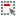
\includegraphics[width=\iconsize]{Figures/Icons/pqSelectMinus16}	& Subtract selection	&&

\includegraphics[width=\iconsize]{Figures/Icons/pqSelectToggle16}	& Toggle selection
\end{tabularx}

In a second step the kind of item, cells or points, to be selected has to be specified:

\begin{tabularx}{\linewidth}{lXclXcl}
Points: &&
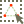
\includegraphics[width=\iconsize]{Figures/Icons/pqSurfaceSelectionPoint24}	& Select points on	&&

\includegraphics[width=\iconsize]{Figures/Icons/pqFrustumSelectionPoint24}	& Select points through	\\
&&
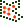
\includegraphics[width=\iconsize]{Figures/Icons/pqPolygonSelectSurfacePoint24}	& Select points with polygon	&&
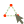
\includegraphics[width=\iconsize]{Figures/Icons/pqSurfaceSelectionPointInteractive}	& Select points interactive	\\
% 
Cells: &&
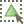
\includegraphics[width=\iconsize]{Figures/Icons/pqSurfaceSelectionCell24}	& Select cells on	&&

\includegraphics[width=\iconsize]{Figures/Icons/pqFrustumSelectionCell24}	& Select cells through	\\
&&
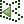
\includegraphics[width=\iconsize]{Figures/Icons/pqPolygonSelectSurfaceCell24.png}	& Select cells with polygon	&&
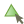
\includegraphics[width=\iconsize]{Figures/Icons/pqSurfaceSelectionCellInteractive}	& Select cells interactive
\end{tabularx}

Selection steps can be repeated as long as no Filter dependent on the selection is active. The currently selected entities are highlighted.

\levelstay{Limit display to selection}
\label{sec:Use_ParaView_Selection_LimitTo}

To limit the model to a user defined selection:

\begin{enumerate}[noitemsep]
\item Import result file to \marktool{\paraviewname}
\item Create a selection
\item From the menu bar:
  \begin{itemize}[noitemsep]
  \item Click Filters
  \item Click Data Analysis
  \item Click \textit{Extract Selection}
  \end{itemize}
  or click 
\includegraphics[width=\iconsize]{Figures/Icons/pqExtractSelection24} in the Data Analysis toolbar
\item Click \textit{Apply} in the newly opened Properties tab
\end{enumerate}

\levelstay{Remarks}

\begin{enumerate}[noitemsep]
   \item  Selected points lie in a virtual box. If the deformation of the model are to big, the points move outside the box and the allocation is lost. This might be an issue for plotting data. This can be solved by setting the deformation scaling to zero.
\end{enumerate}


\newpage
%%%%%%%%%%%%%%%%%%%%%%%%%%%%%%%%%%%%
% Header                           %
%%%%%%%%%%%%%%%%%%%%%%%%%%%%%%%%%%%%
% 
% Revisions: 2017-04-10 Martin R�del <martin.raedel@dlr.de>
%                       Initial draft
%               
% Contact:   Martin R�del,  martin.raedel@dlr.de
%            DLR Composite Structures and Adaptive Systems
%          
%                                 __/|__
%                                /_/_/_/  
%            www.dlr.de/fa/en      |/ DLR
% 
%%%%%%%%%%%%%%%%%%%%%%%%%%%%%%%%%%%%
% Content                          %
%%%%%%%%%%%%%%%%%%%%%%%%%%%%%%%%%%%%

\levelup{View \& Display}
%%%%%%%%%%%%%%%%%%%%%%%%%%%%%%%%%%%%
% Header                           %
%%%%%%%%%%%%%%%%%%%%%%%%%%%%%%%%%%%%
% 
% Revisions: 2017-04-10 Martin R�del <martin.raedel@dlr.de>
%                       Initial draft
%               
% Contact:   Martin R�del,  martin.raedel@dlr.de
%            DLR Composite Structures and Adaptive Systems
%          
%                                 __/|__
%                                /_/_/_/  
%            www.dlr.de/fa/en      |/ DLR
% 
%%%%%%%%%%%%%%%%%%%%%%%%%%%%%%%%%%%%
% Content                          %
%%%%%%%%%%%%%%%%%%%%%%%%%%%%%%%%%%%%

\leveldown{Save view}
\label{sec:Paraview:View:Save}

To save a view configuration click an the \textit{Adjust Camera} button 
\includegraphics[width=\iconsize]{Figures/Icons/pqEditCamera16.png} in the icon bar of your \textit{RenderView}.
%%%%%%%%%%%%%%%%%%%%%%%%%%%%%%%%%%%%
% Header                           %
%%%%%%%%%%%%%%%%%%%%%%%%%%%%%%%%%%%%
% 
% Revisions: 2017-04-10 Martin R�del <martin.raedel@dlr.de>
%                       Initial draft
%               
% Contact:   Martin R�del,  martin.raedel@dlr.de
%            DLR Composite Structures and Adaptive Systems
%          
%                                 __/|__
%                                /_/_/_/  
%            www.dlr.de/fa/en      |/ DLR
%
%%%%%%%%%%%%%%%%%%%%%%%%%%%%%%%%%%%%
% Content                          %
%%%%%%%%%%%%%%%%%%%%%%%%%%%%%%%%%%%%

\levelstay{Display point/node numbers}
\label{sec:Paraview:Display:Point:Labels}

After importing the model it might be of interest to get the node/point numbers for the whole model or a specific selection. To show these numbers after importing the model:

\begin{enumerate}[noitemsep]
  \item Generate and extract the selection of interest according to \autoref{sec:Use_ParaView_Selection}
  \item Left-click on the imported model (set the model active)
  \item From the menubar:
    \begin{itemize}[noitemsep]
      \item Click \textit{View}
      \item Click \textit{Selection Display Inspector}
    \end{itemize}
  \item In the \textit{Selection Display Inspector} window:
    \begin{itemize}[noitemsep]
      \item Click on \textit{Point Labels}
      \item Select \textit{ID}
    \end{itemize}
  \item The point/node numbers appear as labels
\end{enumerate}

\begin{figure}[htbp]
\centering
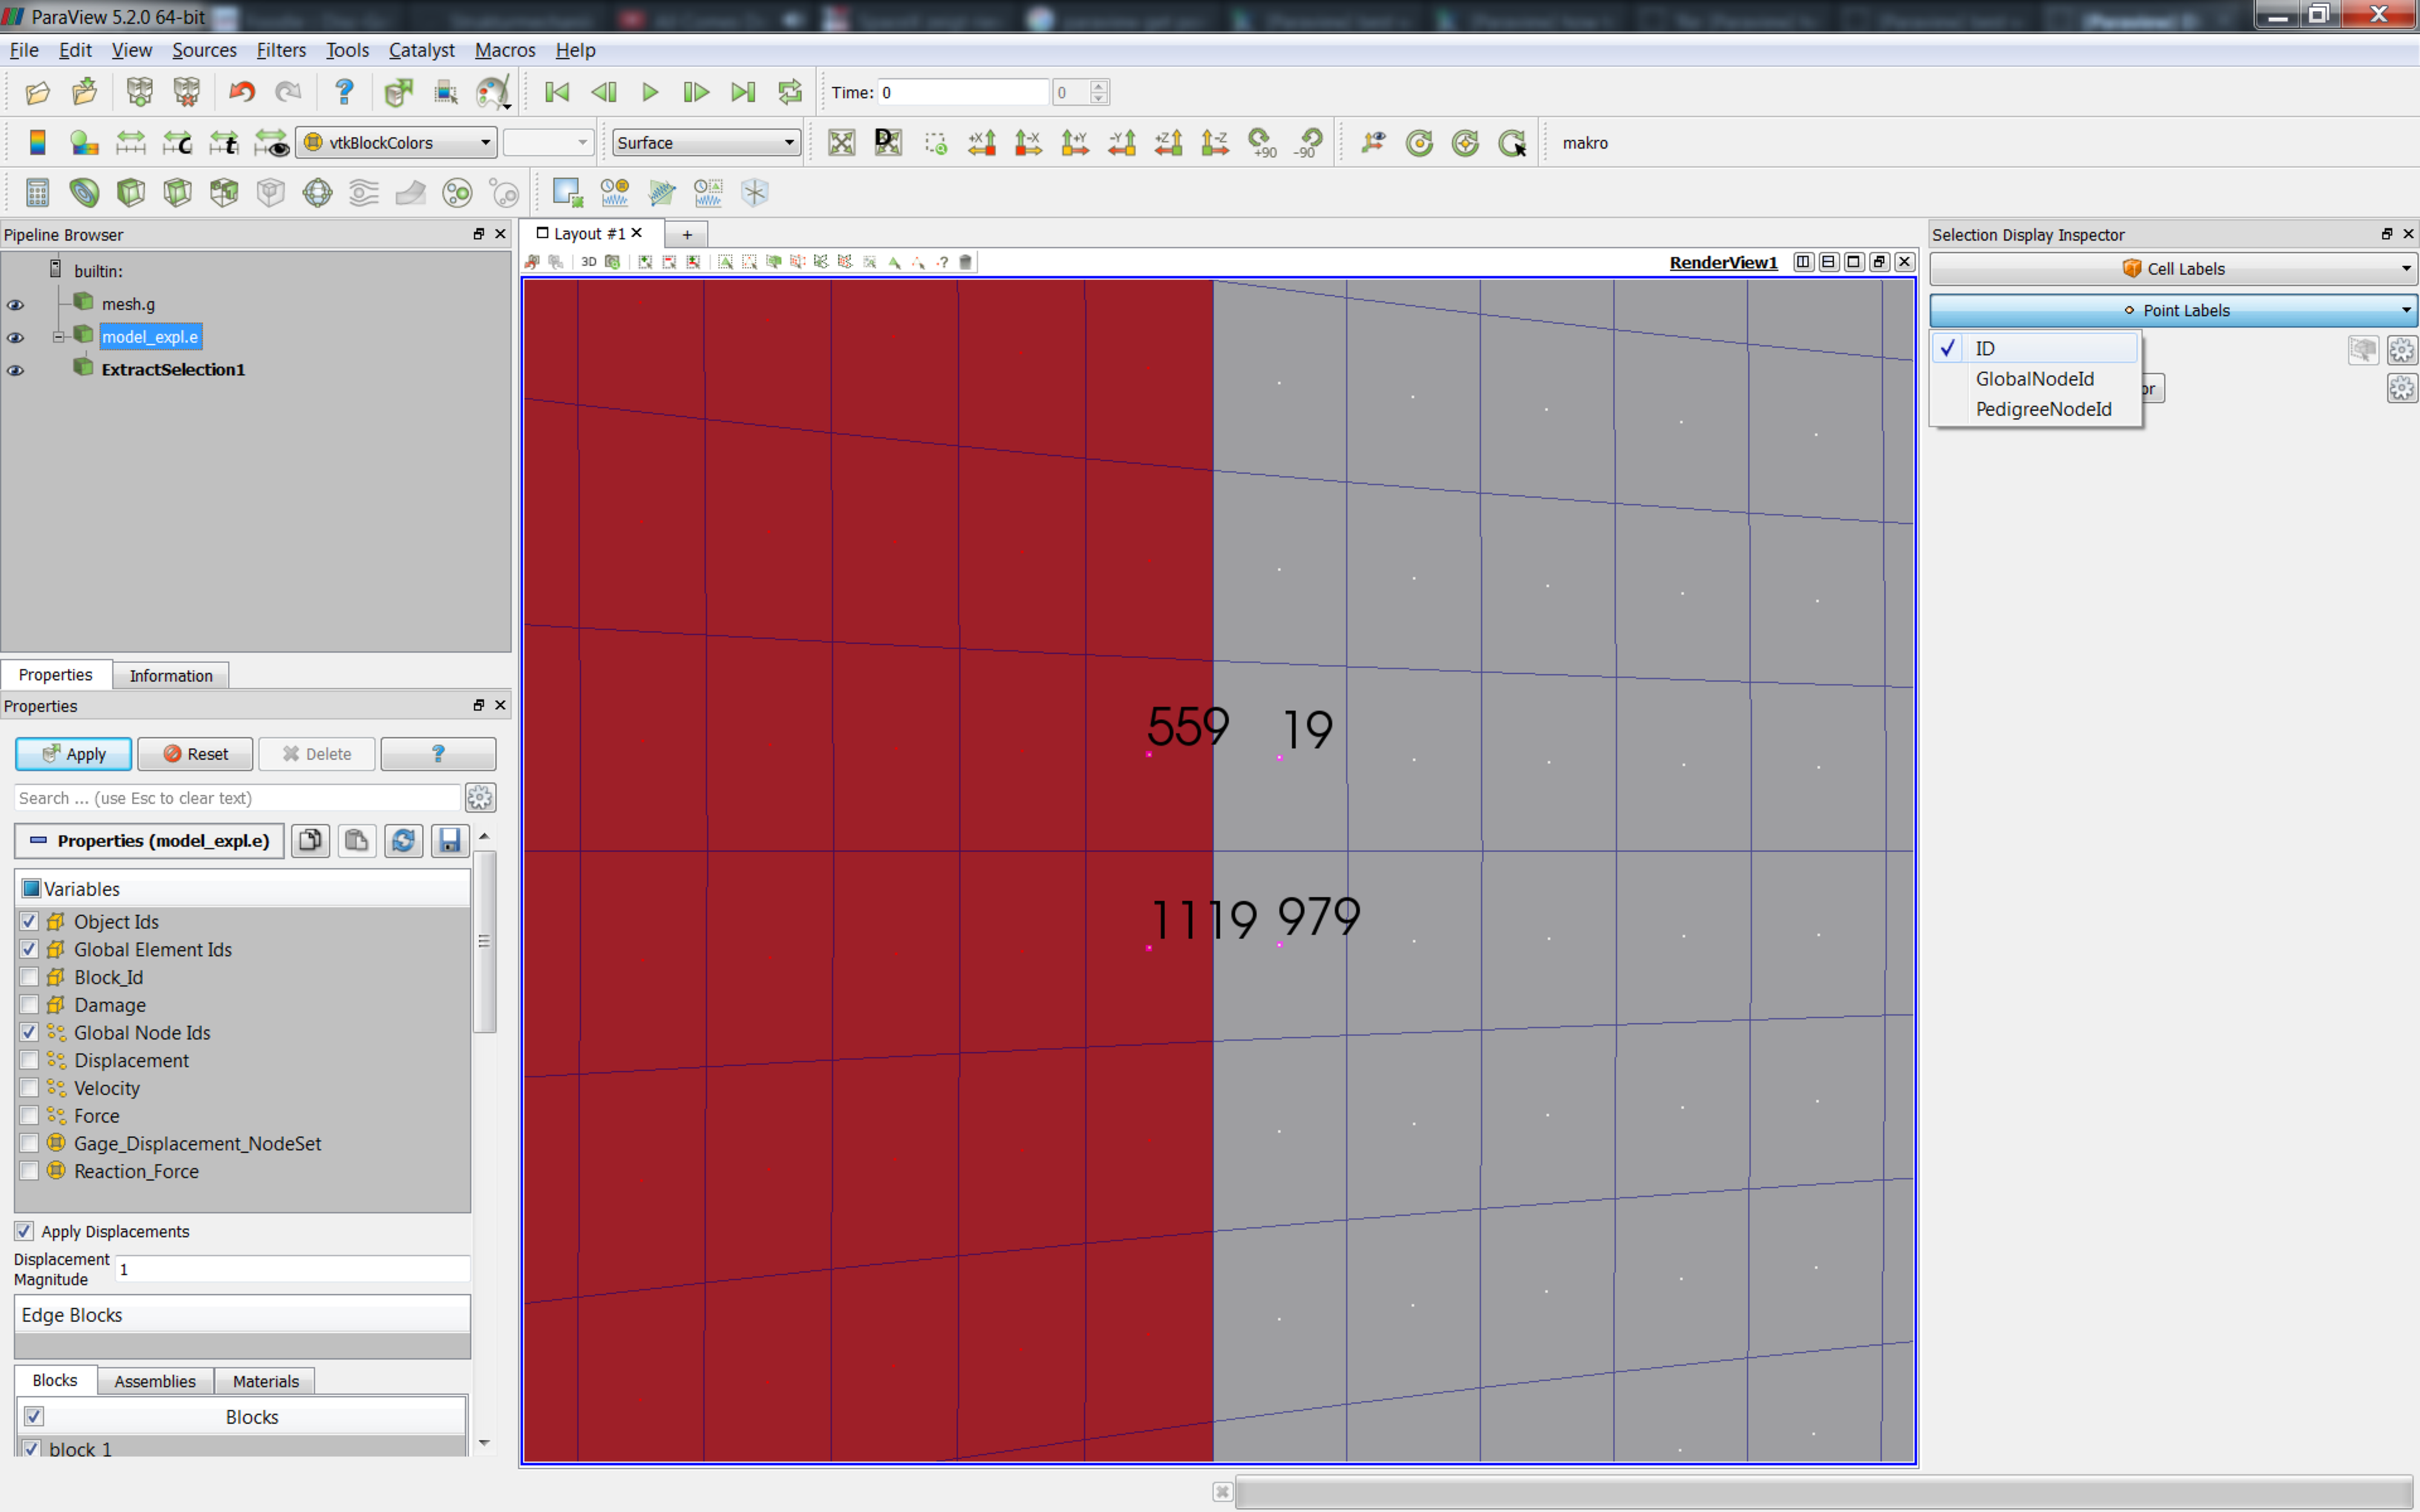
\includegraphics[width=\paraviewscreenshotwidthfac\linewidth]{Figures/Screenshots/ParaView_Display_NodeLabels}
\caption{Display of selection point/node numbers}
\label{fig:Use_ParaView_Display_NodeLabels}
\end{figure}

%%%%%%%%%%%%%%%%%%%%%%%%%%%%%%%%%%%%
% Header                           %
%%%%%%%%%%%%%%%%%%%%%%%%%%%%%%%%%%%%
% 
% Revisions: 2017-04-10 Martin R�del <martin.raedel@dlr.de>
%                       Initial draft
%               
% Contact:   Martin R�del,  martin.raedel@dlr.de
%            DLR Composite Structures and Adaptive Systems
%          
%                                 __/|__
%                                /_/_/_/  
%            www.dlr.de/fa/en      |/ DLR
% 
%%%%%%%%%%%%%%%%%%%%%%%%%%%%%%%%%%%%
% Content                          %
%%%%%%%%%%%%%%%%%%%%%%%%%%%%%%%%%%%%

\levelstay{Visualize nodesets}

To visualize the nodesets from a \marktool{\exodusname} mesh or \marktool{\toolname} results file in \marktool{\paraviewname} perform the following steps

\begin{enumerate}[noitemsep]
\item From the menu bar: \label{itm:Use_ParaView_Visualize_NoseSet_Step1}
  \begin{itemize}[noitemsep]
  \item Click File
  \item Click Open
  \item Select the .g/.e-\marktool{\toolname} input or output file
  \end{itemize}
  or click 
\includegraphics[width=\iconsize]{Figures/Icons/pqOpen32} in the Main Controls toolbar
\item In the newly opened \textit{Properties} tab:
  \begin{itemize}[noitemsep]
  \item Click the gear symbol 
\includegraphics[width=\iconsize]{Figures/Icons/pqAdvanced26} next to the \textit{Search} line
  \item \textit{Sets} and \textit{Maps} tables become available for selection
  \item Select the nodesets to display
  \item Unselect all Blocks
  \item Click \textit{Apply}
  \end{itemize}
\item Create a \textit{Glyph} based on the current model as described in \autoref{sec:ParaView_Damage_Plots_on_Nodes_as_Spheres} (without the result data stuff of course)
\item Repeat step \ref{itm:Use_ParaView_Visualize_NoseSet_Step1}
\item In the newly opened \textit{Properties} tab:
  \begin{itemize}[noitemsep]
  \item Select all Blocks
  \item Set the \textit{Opacity} to 0.4
  \item Click \textit{Apply}
  \end{itemize}
\end{enumerate}

Similarly, the nodesets in the peridynamic collocation point translation can be visualized. The following figure shows the base \marktool{\exodusname} finite element mesh in gray. Superimposed with the finite element mesh are the nodes of a finite element nodeset (blue) and the nodeset in the peridynamic translation (green).

\begin{figure}[htbp]
\centering
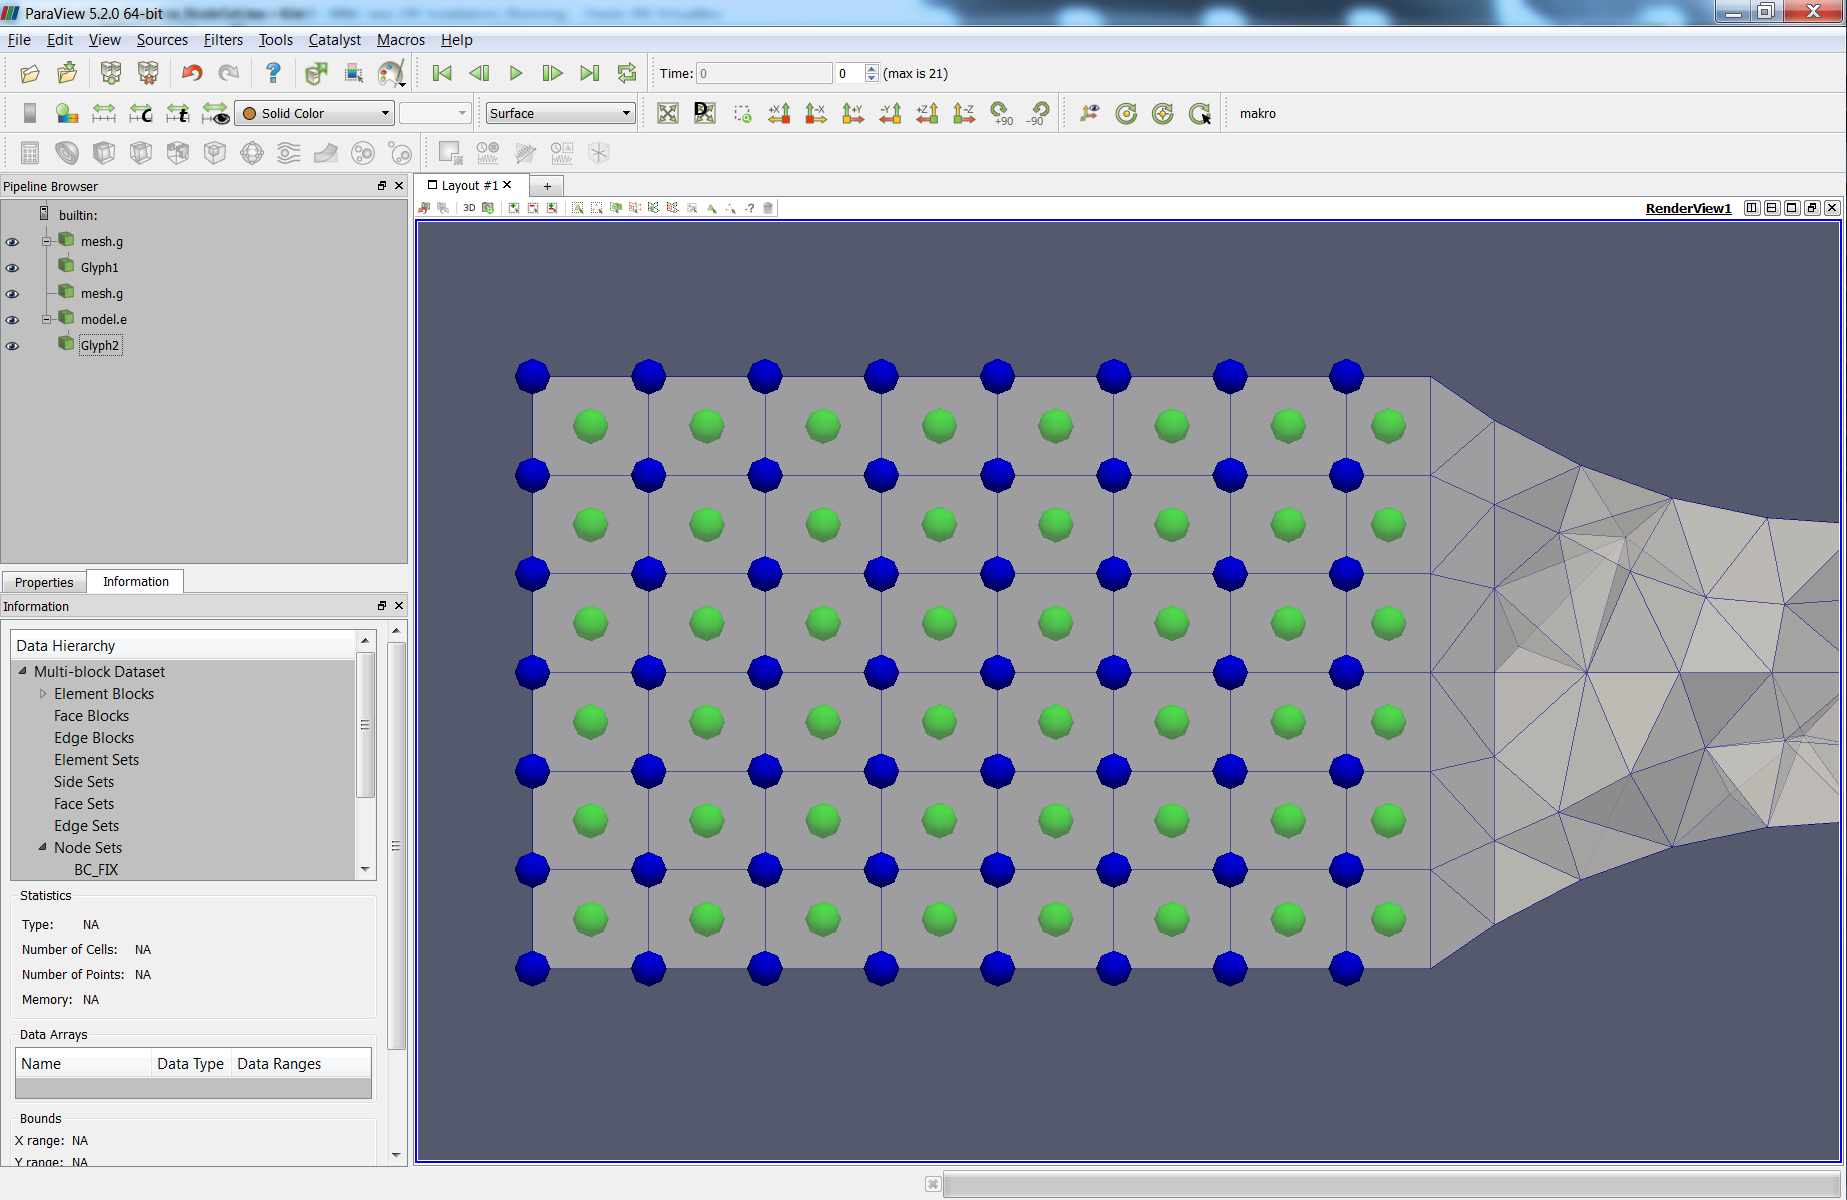
\includegraphics[width=\paraviewscreenshotwidthfac\linewidth]{Figures/Screenshots/ParaView_Visualize_NodeSets}
\caption{Visualization of base finite element mesh (gray), finite element nodeset (blue) and nodeset after transformation to peridynamic collocation points (green)}
\label{fig:Use_ParaView_Visualize_NoseSets}
\end{figure}

\FloatBarrier
%%%%%%%%%%%%%%%%%%%%%%%%%%%%%%%%%%%%
% Header                           %
%%%%%%%%%%%%%%%%%%%%%%%%%%%%%%%%%%%%
% 
% Revisions: 2017-04-10 Martin R�del <martin.raedel@dlr.de>
%                       Initial draft
%               
% Contact:   Martin R�del,  martin.raedel@dlr.de
%            DLR Composite Structures and Adaptive Systems
%          
%                                 __/|__
%                                /_/_/_/  
%            www.dlr.de/fa/en      |/ DLR
% 
%%%%%%%%%%%%%%%%%%%%%%%%%%%%%%%%%%%%
% Content                          %
%%%%%%%%%%%%%%%%%%%%%%%%%%%%%%%%%%%%

\levelstay{Damage plot on nodes as spheres}
\label{sec:ParaView_Damage_Plots_on_Nodes_as_Spheres}

Commonly, the \marktool{\toolname} results are plotted on so called \texttt{Glyphs} in \marktool{\paraviewname}. A \texttt{Glyph} is a geometric object with a specific size, a direction and a color, which is drawn at certain positions within the vector field. \texttt{Glyph} shapes can be an

\begin{multicols}{4}
\begin{itemize}
\addtolength\itemsep{-2ex}
\item Arrow
\item Cone
\item Box
\item Cylinder
\item Line
\item Sphere
\item 2D glyph
\end{itemize}
\end{multicols}

A natural choice for peridynamic nodes is the sphere. Unfortunately, cell data can not be plotted directly in a \texttt{Glyph} plot. Therefore, the cell data has to be converted to point data first.

\begin{enumerate}[noitemsep]
\item Import result file to \marktool{\paraviewname}
\item Left-click on the result file once in the Pipeline Browser (mark the result file)
\item From the menu bar:
  \begin{itemize}[noitemsep]
  \item Click Filters
  \item Click Alphabetical
  \item Click \textit{Cell Data to Point Data}
  \end{itemize}
\item Left-click on the new item \textit{Cell Data to Point Data} in the Pipeline Browser
\item From the menu bar:
  \begin{itemize}[noitemsep]
  \item Click Filters
  \item Click Common
  \item Click \textit{Glyph}
  \end{itemize}
  or choose the \textit{Glyph}-symbol from the common filter icon toolbar
\item In the \textit{Glyph} properties window choose:
  \begin{itemize}[noitemsep]
  \item Glyph Type:	\tab \textit{Sphere}
  \item Scalars:	\tab \textit{Damage}
  \item Vectors:	\tab \textit{Displacement}
  \item Scale factor:	\tab Choose according to your needs
  \item Glyph mode:	\tab \textit{All Points}
  \item Coloring:	\tab \textit{Damage}
  \end{itemize}
  and click \textit{Apply}
\item Afterwards, return to the properties window, go to the \texttt{Display} section and choose:
  \begin{itemize}[noitemsep]
  \item Representation:	\tab \textit{Surface}
  \item Coloring:	\tab \textit{Damage}
  \end{itemize}
\end{enumerate}

Afterwards, you can skip through the time steps of your analysis in the Current Time Controls toolbar. It maybe necessary to adjust the range of the legend to the current time step minimum or maximum.

\newpage
%%%%%%%%%%%%%%%%%%%%%%%%%%%%%%%%%%%%
% Header                           %
%%%%%%%%%%%%%%%%%%%%%%%%%%%%%%%%%%%%
% 
% Revisions: 2017-04-10 Martin R�del <martin.raedel@dlr.de>
%                       Initial draft
%               
% Contact:   Martin R�del,  martin.raedel@dlr.de
%            DLR Composite Structures and Adaptive Systems
%          
%                                 __/|__
%                                /_/_/_/  
%            www.dlr.de/fa/en      |/ DLR
% 
%%%%%%%%%%%%%%%%%%%%%%%%%%%%%%%%%%%%
% Content                          %
%%%%%%%%%%%%%%%%%%%%%%%%%%%%%%%%%%%%

\levelup{Plotting}

%%%%%%%%%%%%%%%%%%%%%%%%%%%%%%%%%%%%
% Header                           %
%%%%%%%%%%%%%%%%%%%%%%%%%%%%%%%%%%%%
% 
% Revisions: 2017-04-10 Martin R�del <martin.raedel@dlr.de>
%                       Initial draft
%               
% Contact:   Martin R�del,  martin.raedel@dlr.de
%            DLR Composite Structures and Adaptive Systems
%          
%                                 __/|__
%                                /_/_/_/  
%            www.dlr.de/fa/en      |/ DLR
%
%%%%%%%%%%%%%%%%%%%%%%%%%%%%%%%%%%%%
% Content                          %
%%%%%%%%%%%%%%%%%%%%%%%%%%%%%%%%%%%%

\leveldown{Plot selection data over time}

To plot selection data, e.g. point results, over calculation time perform the following steps:

\begin{enumerate}[noitemsep]
\item Import result file to \marktool{\paraviewname}
\item Create a selection, e.g. to a single or two points
\item From the menu bar:
  \begin{itemize}[noitemsep]
  \item Click Filters
  \item Click Data Analysis
  \item Click \textit{Plot Selection Over Time}
  \end{itemize}
  or click 
\includegraphics[width=\iconsize]{Figures/Icons/pqPlotSelectionOverTime24} in the Data Analysis toolbar
\item In the newly opened Properties tab:
  \begin{itemize}[noitemsep]
  \item Review the Copied Selection
  \item Click \textit{Apply}
  \item Let \marktool{\paraviewname} process your request a couple of seconds
  \item For the actual values deselect the \textit{Only Report Selection Statistics} checkbox
  \item Click \textit{Apply}
  \item Wait until the progressbar in the bottom right is completed
  \item Select from the selection entities the items you are currently interested in
  \item Choose the \textit{Series Parameters} you are interested in (there is the same quantity for each selection entity, so a couple of times if you have multiple entities in your selection, choose wisely)
  \item Your requested values should show up in the \textit{QuartileChartView}
  \end{itemize}
\item You can skip through the time steps of your analysis in the Current Time Controls toolbar. The current time is shown as the vertical bar in the chart view
\end{enumerate}

To see the actual values in a spreadsheet:

\begin{enumerate}[noitemsep]
\item Right-click on the QuartileChartView top line (where e.g. QuartileChartView1 stands)
\item Create a selection, e.g. to a single or two points
\item Select:
  \begin{itemize}[noitemsep]
  \item Convert To ...
  \item Spreadsheet view
  \end{itemize}
\item In case you want to return to the Chart View you can do so accordingly but you have to repeat the data selection steps mentioned above
\end{enumerate}

A combined view:

\begin{figure}[htbp]
\centering
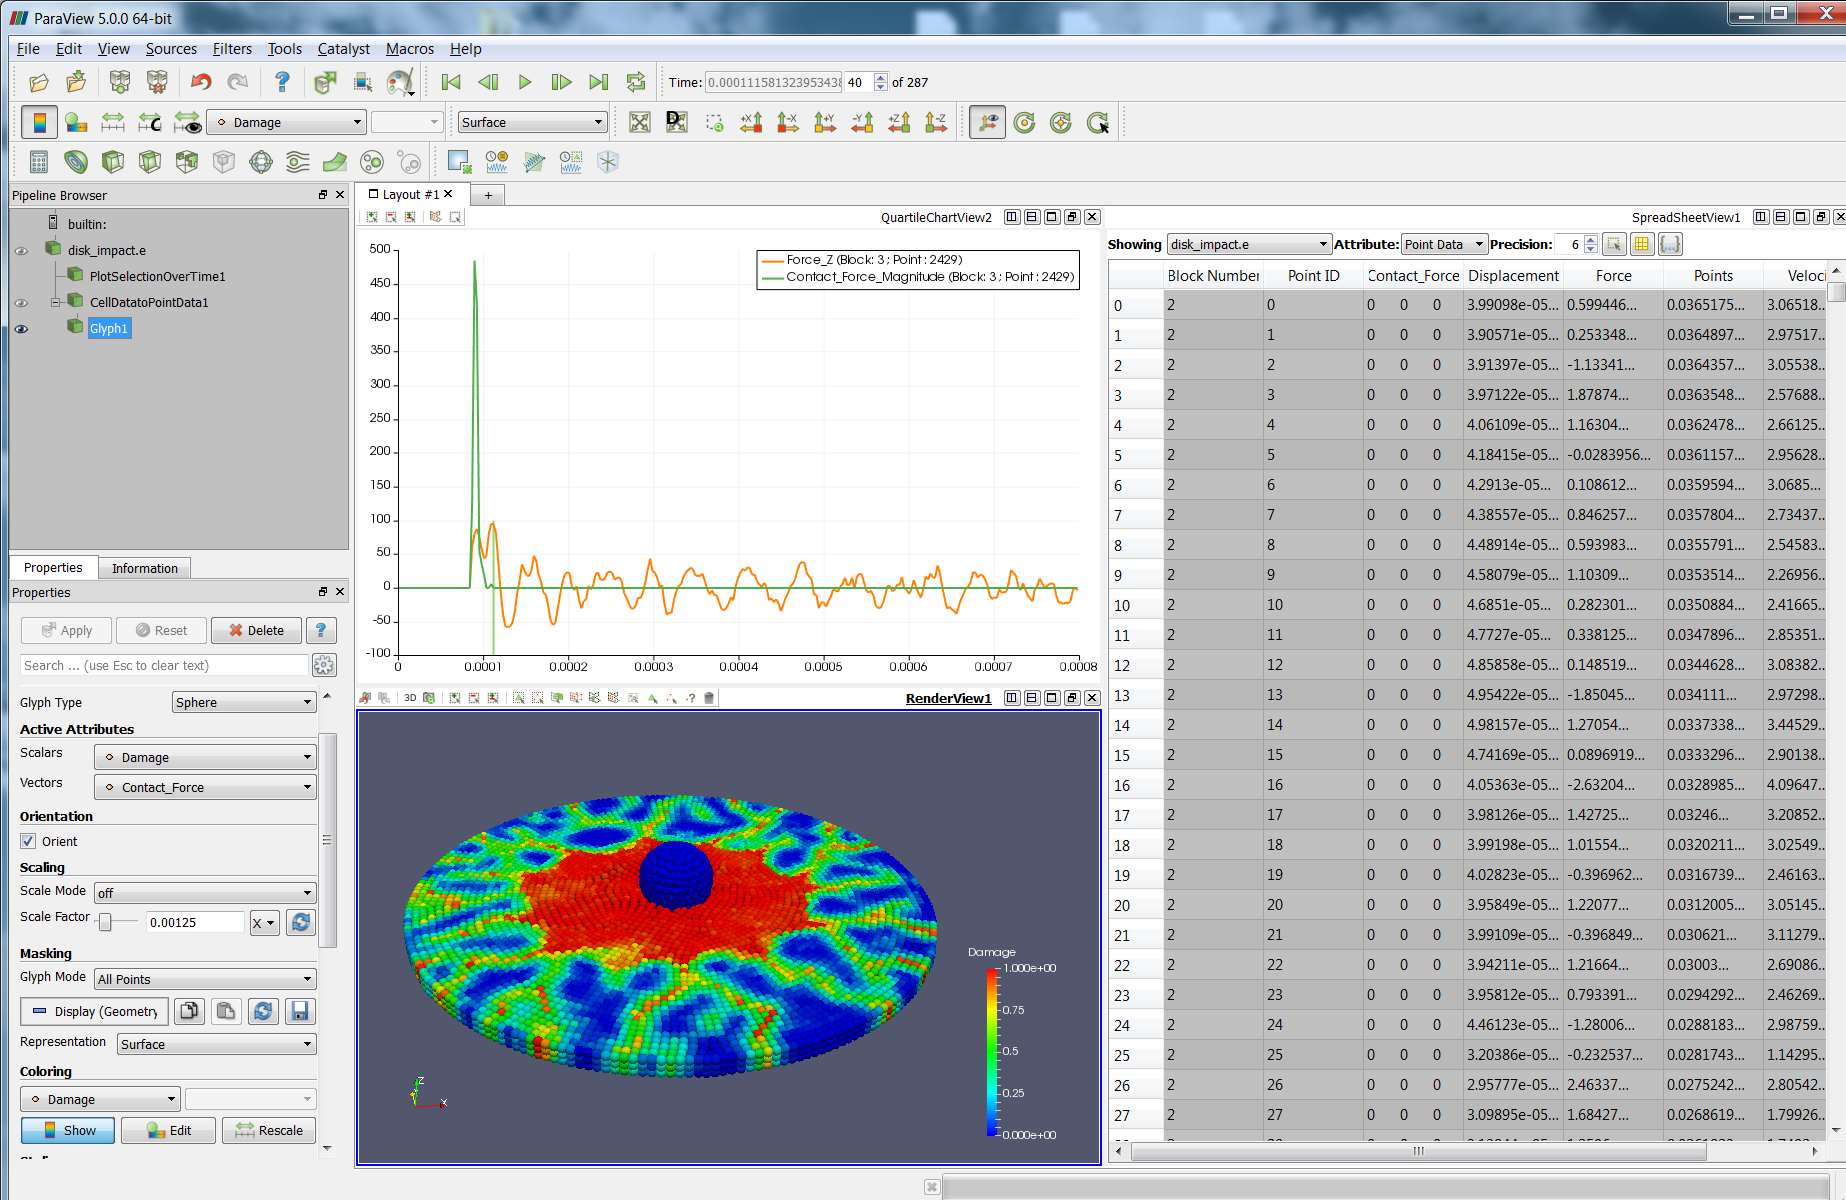
\includegraphics[width=\paraviewscreenshotwidthfac\linewidth]{Figures/Screenshots/State_ChartView_Combined}
\caption{Combined \marktool{\paraviewname} view}
\label{fig:Combined_ParaView_view}
\end{figure}

To save the data for plotting in \verb+pgfplots+:

\begin{enumerate}[noitemsep]
\item Select the PlotOverSelection in the \textit{Pipeline Browser} or left click in the ChartView or SpreadsheetView
\item From the menu bar:
  \begin{itemize}[noitemsep]
  \item Click File
  \item Click Save Data
  \end{itemize}
  or click 
\includegraphics[width=\iconsize]{Figures/Icons/pqSave32} in the Main Controls toolbar
\item Select folder and filename
\item Select csv file type
\item Click \textit{Ok}
\end{enumerate}

Beware, an individual csv-file is written for each and every entity in your selection. The file does not include any information on the entity ID or name. Thus, a sequential save-process for each single individual entity is advised. After each save, rename the resulting file.
%%%%%%%%%%%%%%%%%%%%%%%%%%%%%%%%%%%%
% Header                           %
%%%%%%%%%%%%%%%%%%%%%%%%%%%%%%%%%%%%
% 
% Revisions: 2017-04-10 Martin R�del <martin.raedel@dlr.de>
%                       Initial draft
%               
% Contact:   Martin R�del,  martin.raedel@dlr.de
%            DLR Composite Structures and Adaptive Systems
%          
%                                 __/|__
%                                /_/_/_/  
%            www.dlr.de/fa/en      |/ DLR
% 
%%%%%%%%%%%%%%%%%%%%%%%%%%%%%%%%%%%%
% Content                          %
%%%%%%%%%%%%%%%%%%%%%%%%%%%%%%%%%%%%

\levelstay{Force-displacement-plots}

\leveldown{General}

This plot shows the course of the ``nodal'' force in a constrained region of the model over the displacement of a discrete point. The sum of the forces is used as a representative of the integral force value a load cell would show. For the displacement the value of a discrete node or collocation point is used as a representative for the scalar value of an extensiometer or the machine displacement value.

\levelstay{\protect\toolname/\protect\paraviewname}

\leveldown{Requisition of output values in \protect\toolname}

To acquire forces and displacements for a defined part of a model \texttt{Compute Class Parameters} are used in \toolname. They are described in sections \ref{sec:Peridigm:QRG:ComputeClassParameters:Nodeset}, \ref{sec:Peridigm:QRG:ComputeClassParameters:Block} \& \ref{sec:Peridigm:QRG:ComputeClassParameters:NearestPoint}. The forces are requested for the node set or block where a body load or in this case boundary condition is applied on. The displacement is written for one point in this node set using the nearest neighbor approach to a defined spatial coordinate in the node set region. The initial position of the point the displacements are written for is also requested for convenience and checks.

\begin{code}
Compute Class Parameters
  Strain Gage Initial Position
    Compute Class "Nearest_Point_Data"
    X 0.0317
    Y 1.238
    Z 0.0
    Variable "Model_Coordinates"
    Output Label "Gage_Initial_Position"
    Verbose "True"
  Strain Gage Displacement
    Compute Class "Nearest_Point_Data"
    X 0.0317
    Y 1.238
    Z 0.0
    Variable "Displacement"
    Output Label "Gage_Displacement"
    Verbose "True"
  Reaction Force
    Compute Class "Node_Set_Data"
    Calculation Type "Sum"
    Node Set "bc_load"
    Variable "Force"
    Output Label "Reaction_Force"
\end{code}

Alternatively, it should also be possible to request the displacement for the same node set as the force and simply choose ``Minimum'' or ``Maximum'' as \textit{Calculation type}. This way, it is not required to adjust the spatial coordinates as in \textit{Compute Class ``Nearest\_Point\_Data''}. This works fine for a test case.

Additionally the global output variable types \textit{Displacement} and \textit{Force} must be requested in the output section.

\begin{code}
Output
  Output File Type "ExodusII"
  Output Filename "model"
  Output Frequency 1
  Output Variables
    ...
    Displacement "true"
    ...
    Force "true"
    ...
    Gage_Initial_Position "true"
    Gage_Displacement "true"
    Reaction_Force "true"
\end{code}

\levelstay{Access result data in \protect\paraviewname}

\begin{figure}[htbp]
\centering
  \begin{subfigure}{0.49\linewidth}
    \centering
    \begin{tikzpicture}
      % External figure
      \node[anchor=south west,inner sep=0] (image) at (0,0) {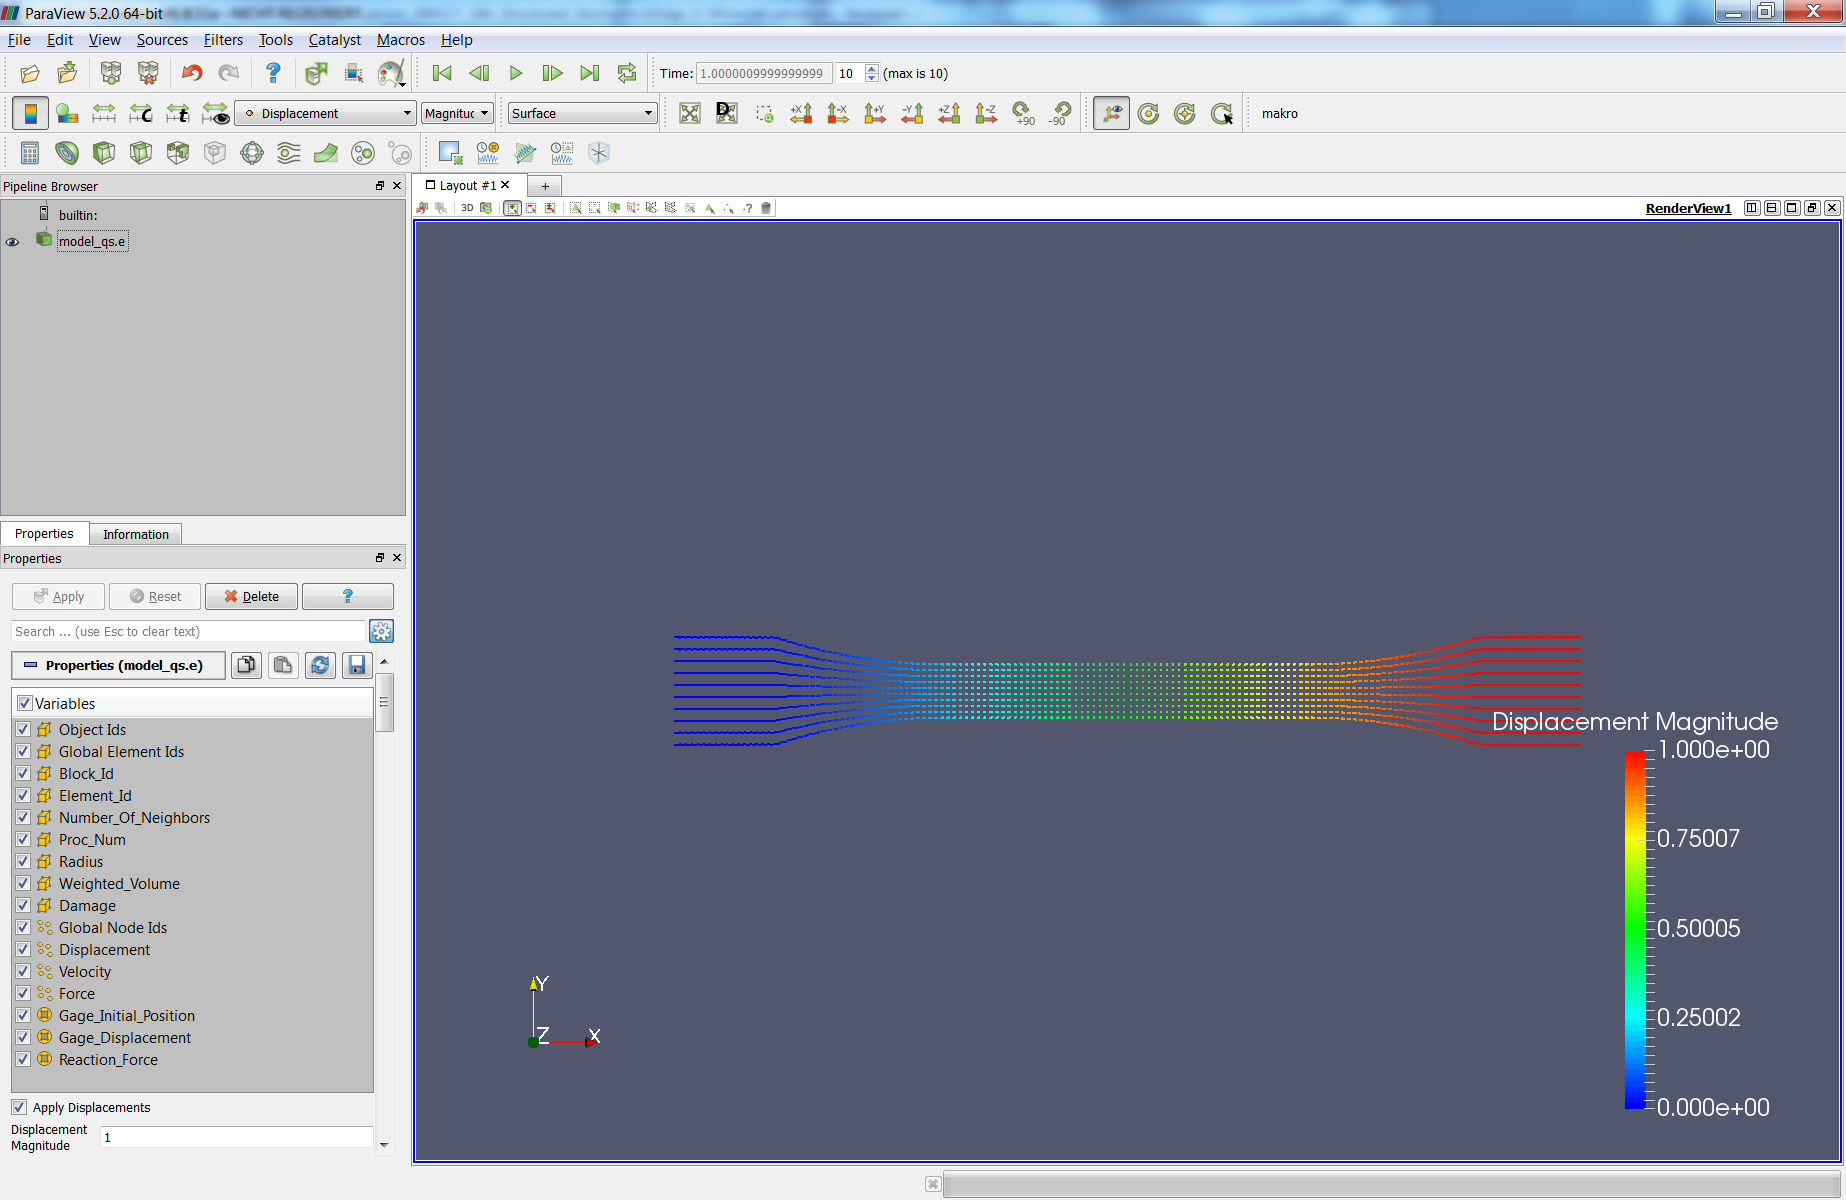
\includegraphics[width=\linewidth]{Figures/Screenshots/ParaView_ComputeClassParameter_ResultsData_1}};
      \begin{scope}[
        x={(image.south east)},
        y={(image.north west)},
      ]
        % Some label
        \node[fit={(0.007,0.10) (0.18,0.17)},myrectangularmarkup] (rect1) {};
        \node[anchor=west,mymarkuptext] (rect1label) at (rect1.east) {1};
        %
        \node[fit={(0.280,0.83) (0.31,0.86)},myrectangularmarkup] (rect2) {};
        \node[anchor=west,mymarkuptext] (rect2label) at (rect2.east) {2};
        % Help grid and labels
        %\pic{myimagegrid};
      \end{scope}
      % Outside label
    \end{tikzpicture}
    \caption{Steps 1-2}
    \label{fig:ParaView_ComputeClassParameter_ResultsData_1}
  \end{subfigure}%
  %\\
  \hfill
  \begin{subfigure}{0.49\linewidth}
    \centering
    \begin{tikzpicture}
      % External figure
      \node[anchor=south west,inner sep=0] (image) at (0,0) {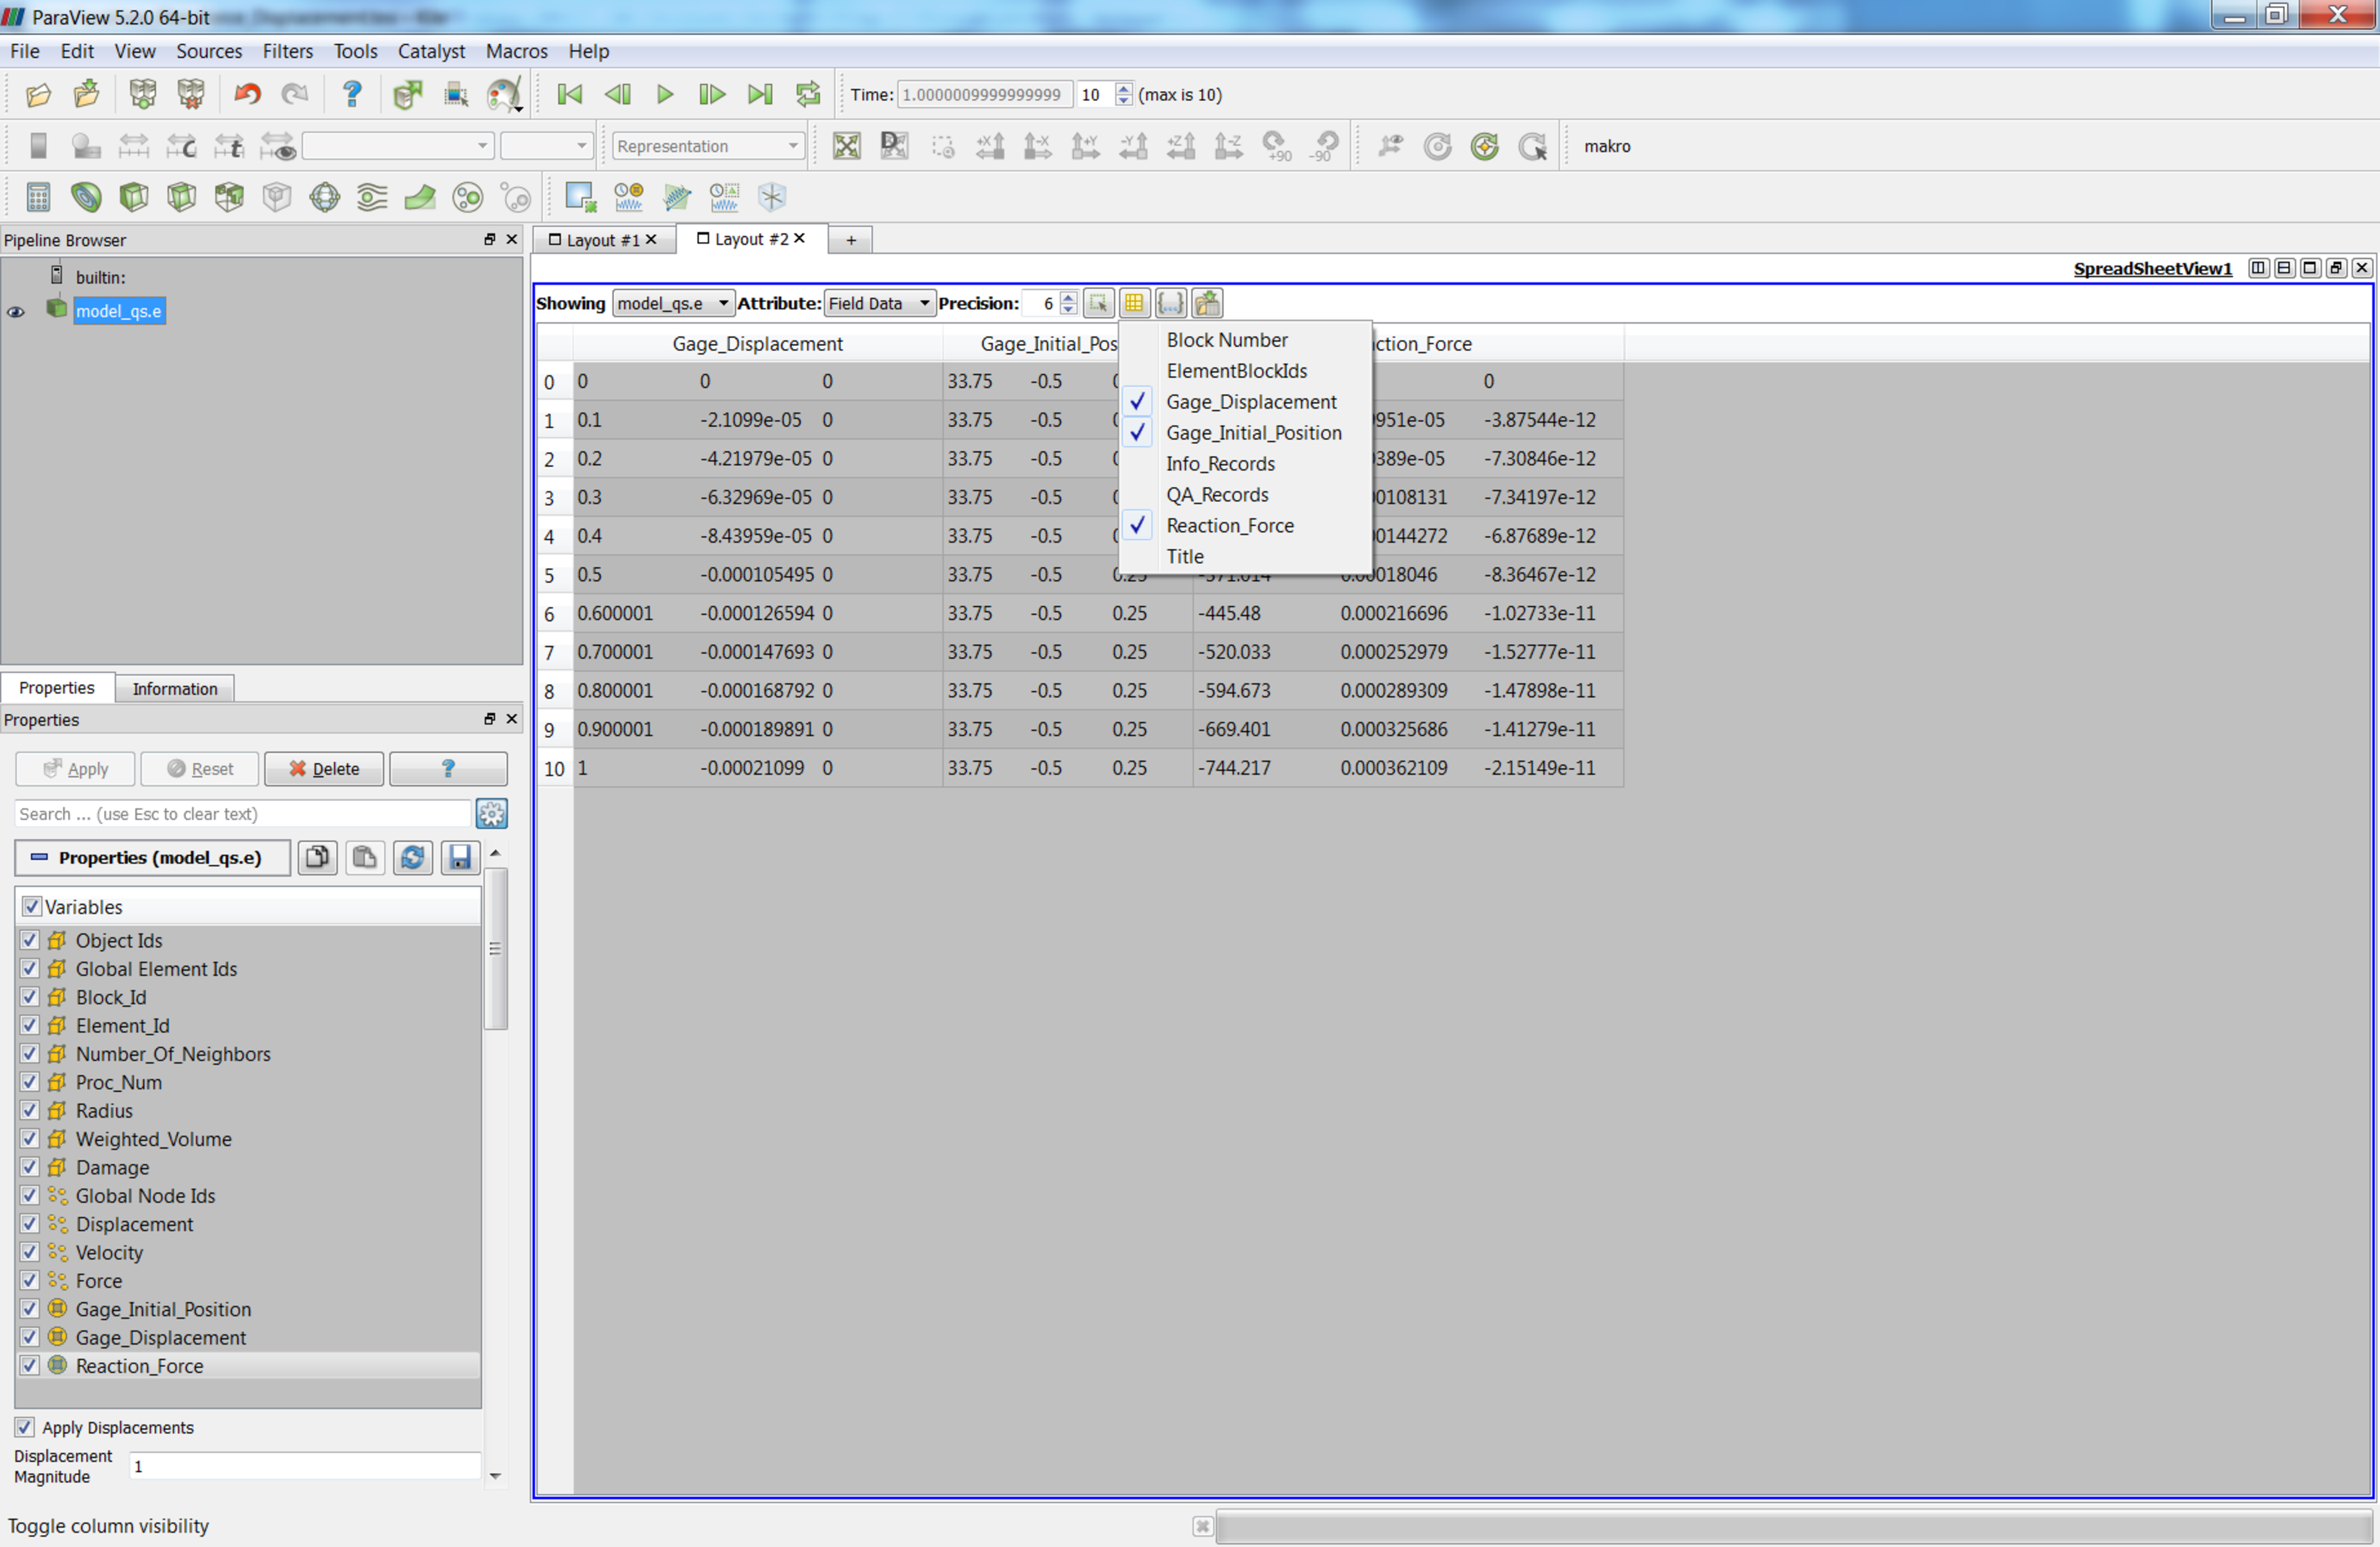
\includegraphics[width=\linewidth]{Figures/Screenshots/ParaView_ComputeClassParameter_ResultsData_2}};
      \begin{scope}[
        x={(image.south east)},
        y={(image.north west)},
      ]
        % Some label
        \node[fit={(0.22,0.785) (0.40,0.82)},myrectangularmarkup] (rect3) {};
        \node[anchor=north,mymarkuptext] (rect3label) at (rect3.south) {3};
        %
        \node[fit={(0.465,0.62) (0.585,0.82)},myrectangularmarkup] (rect4) {};
        \node[anchor=west,mymarkuptext] (rect4label) at (rect4.east) {4};
        % Help grid and labels
        %\pic{myimagegrid};
      \end{scope}
      % Outside label
    \end{tikzpicture}
    \caption{Steps 3-4}
    \label{fig:ParaView_ComputeClassParameter_ResultsData_2}
  \end{subfigure}%
\caption{Access \texttt{Compute Class Parameters} results data in \protect\paraviewname}
\label{fig:Use_ParaView_ComputeClassParameter_ResultsData}
\end{figure}

\begin{enumerate}[noitemsep]
  \item Make sure that the requested result data from the \textit{Compute Class Parameters} is available in your results file. If you are only interested in these parameters, unselect all other.
  \item Add a new view \& select \textit{SpreadSheet View}
  \item For \textit{Showing} select your model and for \textit{Attribute} select \textit{Field Data}
  \item Click 
\includegraphics[width=\iconsize]{Figures/Icons/pqRectilinearGrid16} to select the columns of interest
  \item Click 
\includegraphics[width=\iconsize]{Figures/Icons/pqSaveTable32} to save the spreadsheet data as a \texttt{csv}-file
  \begin{enumerate}[noitemsep]
    \item Specify a filename \& click \textit{Ok}
    \item In the next dialog toggle \textit{Filter Columns by Visibility}. Otherwise, all data is written to the \texttt{csv}-file.
  \end{enumerate}
  \item Do with the data whatever you want \smiley
\end{enumerate}

\levelstay{Plot result data directly in \protect\paraviewname}

\begin{figure}[htbp]
\centering
    \begin{tikzpicture}
      % External figure
      \node[anchor=south west,inner sep=0] (image) at (0,0) {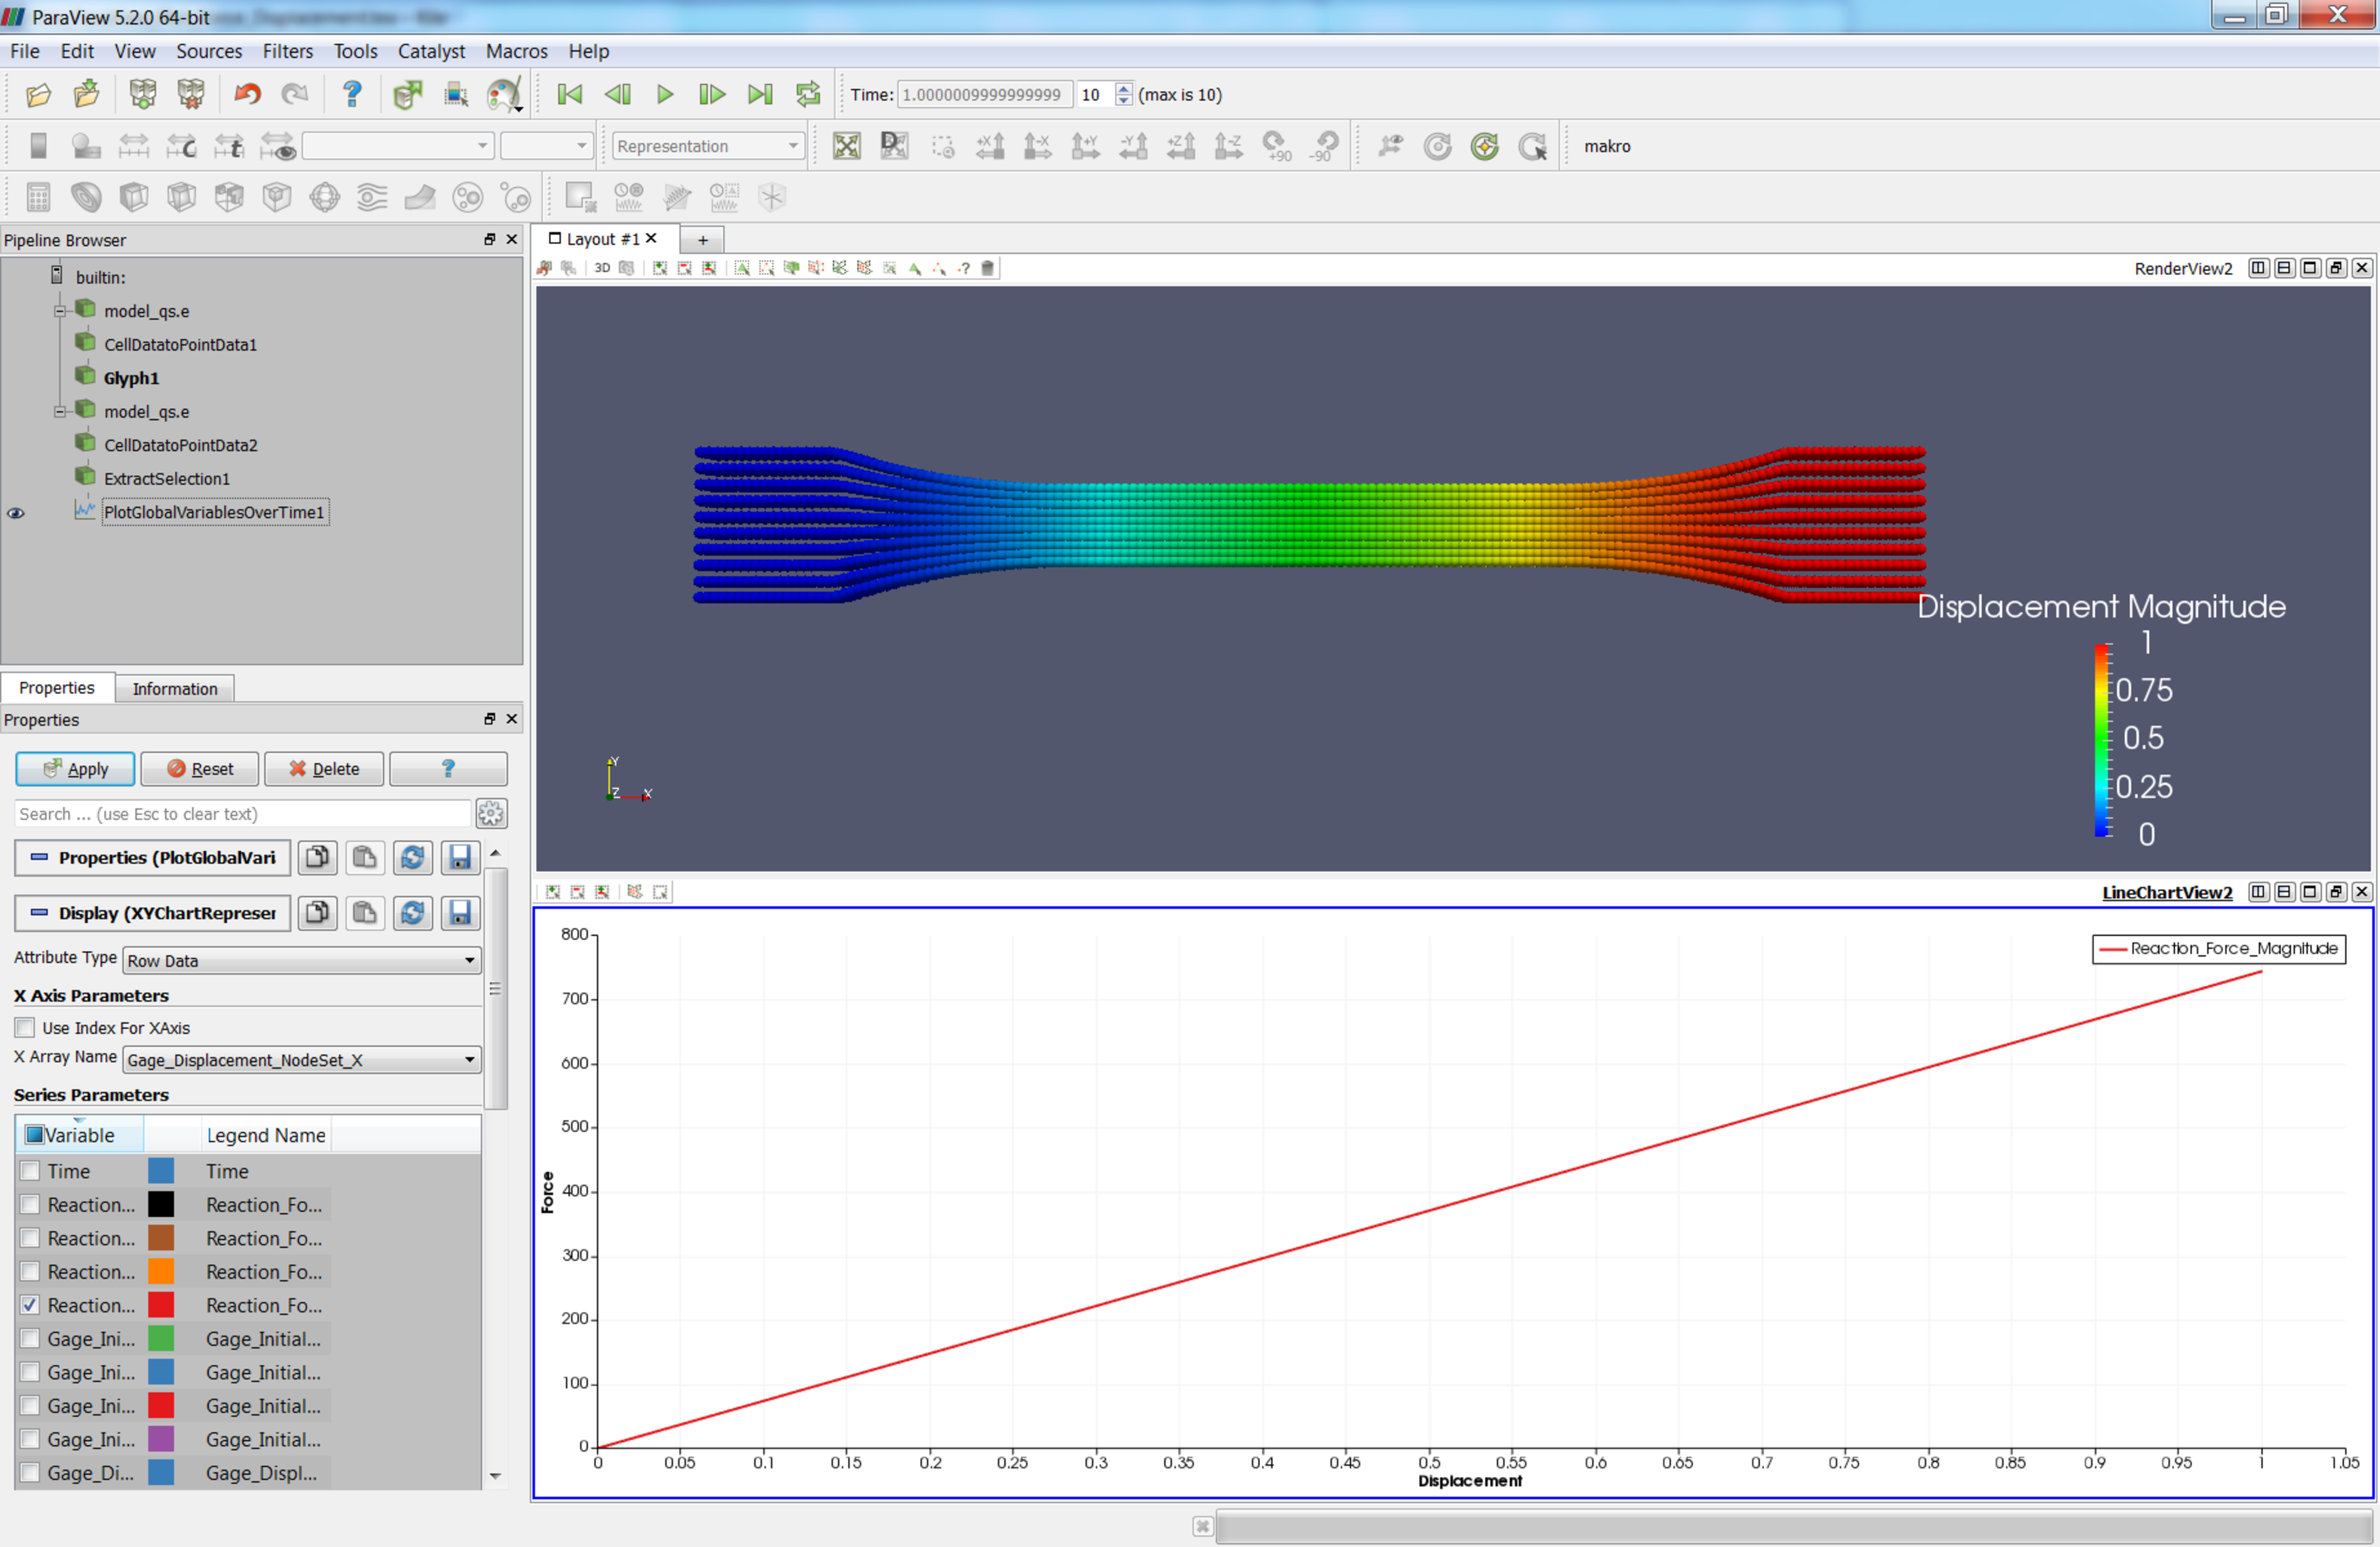
\includegraphics[width=0.8\linewidth]{Figures/Screenshots/ParaView_ComputeClassParameter_ResultsData_3}};
      \begin{scope}[
        x={(image.south east)},
        y={(image.north west)},
      ]
        % Some label
%         \node[fit={(0.007,0.10) (0.18,0.17)},myrectangularmarkup] (rect1) {};
%         \node[anchor=west,mymarkuptext] (rect1label) at (rect1.east) {1};
%         %
%         \node[fit={(0.280,0.83) (0.31,0.86)},myrectangularmarkup] (rect2) {};
%         \node[anchor=west,mymarkuptext] (rect2label) at (rect2.east) {2};
        % Help grid and labels
%         \pic{myimagegrid};
      \end{scope}
    \end{tikzpicture}
\caption{Plot \texttt{Compute Class Parameters} results data in \protect\paraviewname}
\label{fig:Use_ParaView_ComputeClassParameter_ResultsData_ForceDisplacement_in-ParaView}
\end{figure}

\begin{enumerate}[noitemsep]
  \item Import your model
  \item Make sure that the requested result data from the \textit{Compute Class Parameters} is available in your results file. If you are only interested in these parameters, unselect all other.
  \item From the menu bar:
    \begin{itemize}[noitemsep]
    \item Click Filters
    \item Click Alphabetical
    \item Click \textit{Cell Data to Point Data}
    \end{itemize}
  \item Select points of interest:
    \begin{itemize}[noitemsep]
    \item Select the \textit{Cell Data to Point Data} entry in the Pipeline Browser
    \item Create a new selection of a single or multiple points in your constraint region as described in \autoref{sec:Use_ParaView_Selection_Create}
    \item Extract the selection as described in \autoref{sec:Use_ParaView_Selection_LimitTo}
    \end{itemize}
  \item From the menu bar:
    \begin{itemize}[noitemsep]
    \item Click Filters
    \item Click Data Analysis
    \item Click \textit{Plot Selection Over Time}
    \end{itemize}
    or click 
\includegraphics[width=\iconsize]{Figures/Icons/pqPlotSelectionOverTime24} in the Data Analysis toolbar
  \item Preferences in the \textit{Properties} window
    \begin{itemize}[noitemsep]
    \item Under \textit{X Axis Parameters} select your displacement component or magnitude from the \texttt{Compute Class Parameters} in the \textit{X Array Name} combobox
    \item For \textit{Series Parameters} select the force value you want to plot from the \texttt{Compute Class Parameters}, either as a component or magnitude
    \item Input a \textit{Left Axis Title} and \textit{Bottom Axis Title} if required
    \end{itemize}
  \item Click \textit{Apply}
  \item In case you want to export the chart data from here:
    \begin{itemize}[noitemsep]
    \item Left-click on the chart
    \item From the menu bar:
      \begin{itemize}[noitemsep]
      \item Click \textit{File}
      \item Click \textit{Save As}
      \item Export as \texttt{csv}-file
      \end{itemize}
    \end{itemize}
\end{enumerate}

\levelup{\protect\abaqusname}

% https://www.youtube.com/watch?v=O8CcSB11468

\leveldown{Standard}

\begin{enumerate}[noitemsep]
  \item Choose Displacement (U) \& Reaction Forces (RF) as field outputs for the step you want to have the plot
  \item Run the analysis
  \item Open the odb
  \item Reaction force over time:
  \begin{enumerate}[noitemsep]
    \item Click \textit{Create XY Data}
    \item Select Source \textit{ODB history output}
    \item Click \textit{Continue}
    \item Select all entries with beginning \textit{Reation force:} of the nodeset your are interested in
    \item Click \textit{Save as}
    \item Assign name, here ``RF'', \& in \textit{Save Operation} select \textit{sum((XY,XY,$\ldots$))}
  \end{enumerate}
  \item Displacement over time:
  \begin{enumerate}[noitemsep]
    \item Click \textit{Create XY Data}
    \item Select Source \textit{ODB history output}
    \item Click \textit{Continue}
    \item Select all entries with beginning \textit{Spatial displacement Ui:} of the nodeset your are interested in
    \item Click \textit{Save as}
    \item Assign name, here ``U'', \& in \textit{Save Operation} select \textit{avg((XY,XY,$\ldots$))}
  \end{enumerate}
  \item Reaction force over displacement:
  \begin{enumerate}[noitemsep]
    \item Click \textit{Create XY Data}
    \item Select Source \textit{Operate on XY data}
    \item Click \textit{Continue}
    \item From \textit{Operators} select \textit{Combine}
    \item In the equation, at first select ``U'', than ``RF'', the equation than should be \verb+combine ("U","F")+
    \item Select \textit{Plot Expression}
  \end{enumerate}
\end{enumerate}

\levelstay{Explicit}

\begin{enumerate}[noitemsep]
  \item Choose Displacement (U), Reaction Forces (RF) \& Nodal forces (NFORC) as field outputs for the step you want to have the plot
  \item Run the analysis
  \item Open the odb
  \item Reaction force \& Displacement over time:
  \begin{enumerate}[noitemsep]
    \item Click \textit{Create XY Data}
    \item Select Source \textit{ODB field output}
    \item Click \textit{Continue}
    \item \textit{XY Data from ODB Field Output} dialog:
      \begin{enumerate}[noitemsep]
        \item In the \textit{Variables} tab, select \textit{Unique nodal} in the \textit{Position} combobox and all necessary entry checkboxes, here RF1 and U1
        \item In the \textit{Elements/Nodes} tab, select the requested nodeset
      \end{enumerate}
    \item Click \textit{Save}
  \end{enumerate}
  \item Sum forces:
  \begin{enumerate}[noitemsep]
    \item Click \textit{Create XY Data}
    \item Select Source \textit{Operate on XY data}
    \item From \textit{Operators} select \textit{sum}
    \item In the equation, select all ``RF1'' entries`` and click \textit{Add to expression}
    \item Click \textit{Save as} \& assign name ''RF``
  \end{enumerate}
  \item Average displacements:
  \begin{enumerate}[noitemsep]
    \item Click \textit{Create XY Data}
    \item Select Source \textit{Operate on XY data}
    \item From \textit{Operators} select \textit{avg}
    \item In the equation, select all ``U1'' entries`` and click \textit{Add to expression}
    \item Click \textit{Save as} \& assign name ''U``
  \end{enumerate}
  \item Reaction force over displacement:
  \begin{enumerate}[noitemsep]
    \item Click \textit{Create XY Data}
    \item Select Source \textit{Operate on XY data}
    \item Click \textit{Continue}
    \item From \textit{Operators} select \textit{Combine}
    \item In the equation, at first select ``U'', than ``RF'', the equation than should be \verb+combine ("U","F")+
    \item Select \textit{Plot Expression}
  \end{enumerate}
\end{enumerate}

\levelstay{Save XY data}

\begin{enumerate}[noitemsep]
  \item Open the odb
  \item Create all results
  \item In the menu bar, click \textit{Report}
  \item Click \textit{XY}
  \item Adjust the dialog preferences according to your needs
\end{enumerate}

\newpage
%%%%%%%%%%%%%%%%%%%%%%%%%%%%%%%%%%%%
% Header                           %
%%%%%%%%%%%%%%%%%%%%%%%%%%%%%%%%%%%%
% 
% Revisions: 2017-04-10 Martin R�del <martin.raedel@dlr.de>
%                       Initial draft
%               
% Contact:   Martin R�del,  martin.raedel@dlr.de
%            DLR Composite Structures and Adaptive Systems
%          
%                                 __/|__
%                                /_/_/_/  
%            www.dlr.de/fa/en      |/ DLR
% 
%%%%%%%%%%%%%%%%%%%%%%%%%%%%%%%%%%%%
% Content                          %
%%%%%%%%%%%%%%%%%%%%%%%%%%%%%%%%%%%%

\levelmultiup{Measuring}{3}

%%%%%%%%%%%%%%%%%%%%%%%%%%%%%%%%%%%%
% Header                           %
%%%%%%%%%%%%%%%%%%%%%%%%%%%%%%%%%%%%
% 
% Revisions: 2017-04-10 Martin R�del <martin.raedel@dlr.de>
%                       Initial draft
%               
% Contact:   Martin R�del,  martin.raedel@dlr.de
%            DLR Composite Structures and Adaptive Systems
%          
%                                 __/|__
%                                /_/_/_/  
%            www.dlr.de/fa/en      |/ DLR
% 
%%%%%%%%%%%%%%%%%%%%%%%%%%%%%%%%%%%%
% Content                          %
%%%%%%%%%%%%%%%%%%%%%%%%%%%%%%%%%%%%

\leveldown{Node/point position}

Sometimes it is necessary to get the exact position of a single point or selection of points. The following steps give you these informations and are explained for a selection of points. For an inidividual point some steps can be omitted.

\begin{enumerate}[noitemsep]
  \item Import the model
  \item Generate and extract the selection of interest according to \autoref{sec:Use_ParaView_Selection}
  \item Display the node/point numbers according to \autoref{sec:Paraview:Display:Point:Labels}
  \item Remember the node/point numbers
  \item In the RenderView select \textit{Split Horizontal}
  \item Create a new SpreadSheet View
  \item In the SpreadSheet View:
  \begin{itemize}[noitemsep]
    \item Select your selection in the \textit{Showing} combobox
    \item Select \textit{Point Data} in the \textit{Attribute} combobox
    \item The coordinates appear in the \textit{Points} column of the table
    \item In case not all your selected points appear in the table, check if the blocks the points are part of are selected in the \textit{Properties tab} of your selection
  \end{itemize}
  \item Unfortunately the node/point number labels disappear
\end{enumerate}

\begin{figure}[htbp]
\centering
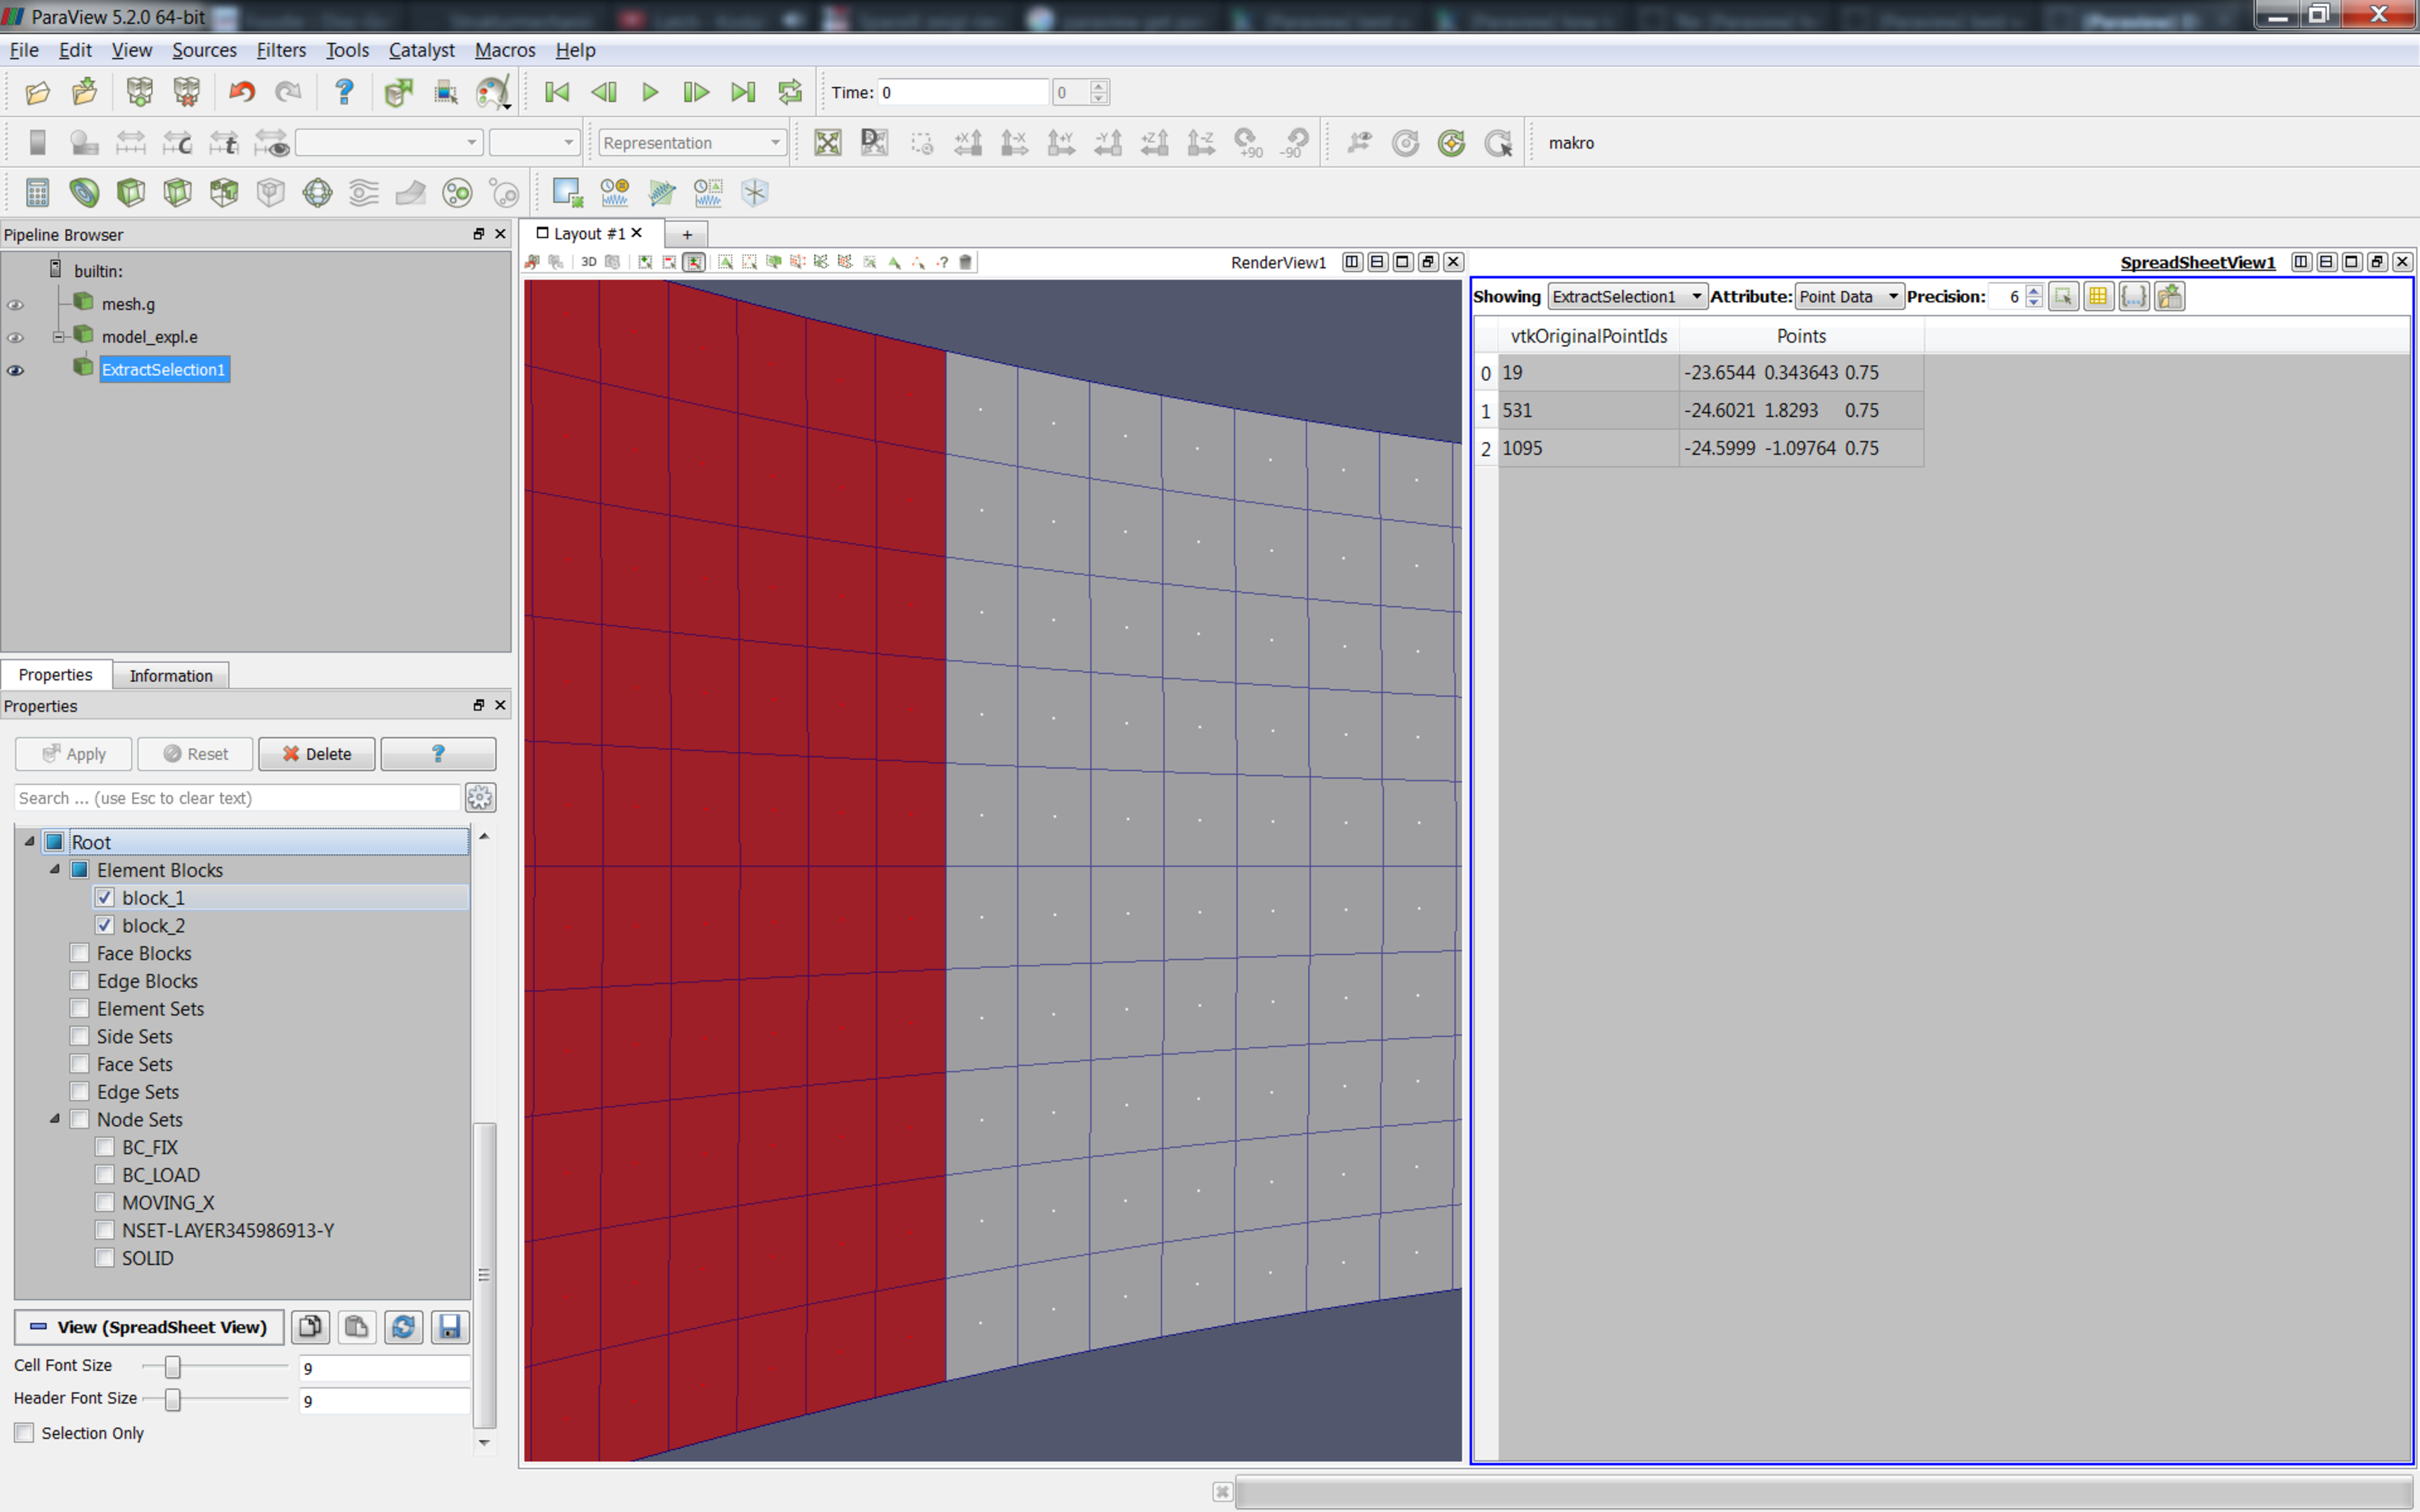
\includegraphics[width=\paraviewscreenshotwidthfac\linewidth]{Figures/Screenshots/ParaView_Display_NodePosition}
\caption{Display of selection point/node positions}
\label{fig:Use_ParaView_Display_NodePositions}
\end{figure}

%%%%%%%%%%%%%%%%%%%%%%%%%%%%%%%%%%%%
% Header                           %
%%%%%%%%%%%%%%%%%%%%%%%%%%%%%%%%%%%%
% 
% Revisions: 2017-04-10 Martin R�del <martin.raedel@dlr.de>
%                       Initial draft
%               
% Contact:   Martin R�del,  martin.raedel@dlr.de
%            DLR Composite Structures and Adaptive Systems
%          
%                                 __/|__
%                                /_/_/_/  
%            www.dlr.de/fa/en      |/ DLR
% 
%%%%%%%%%%%%%%%%%%%%%%%%%%%%%%%%%%%%
% Content                          %
%%%%%%%%%%%%%%%%%%%%%%%%%%%%%%%%%%%%

\levelstay{Node/point distance}

\begin{figure}[htbp]
\centering
  \begin{tikzpicture}
    % External figure
    \node[anchor=south west,inner sep=0] (image) at (0,0) {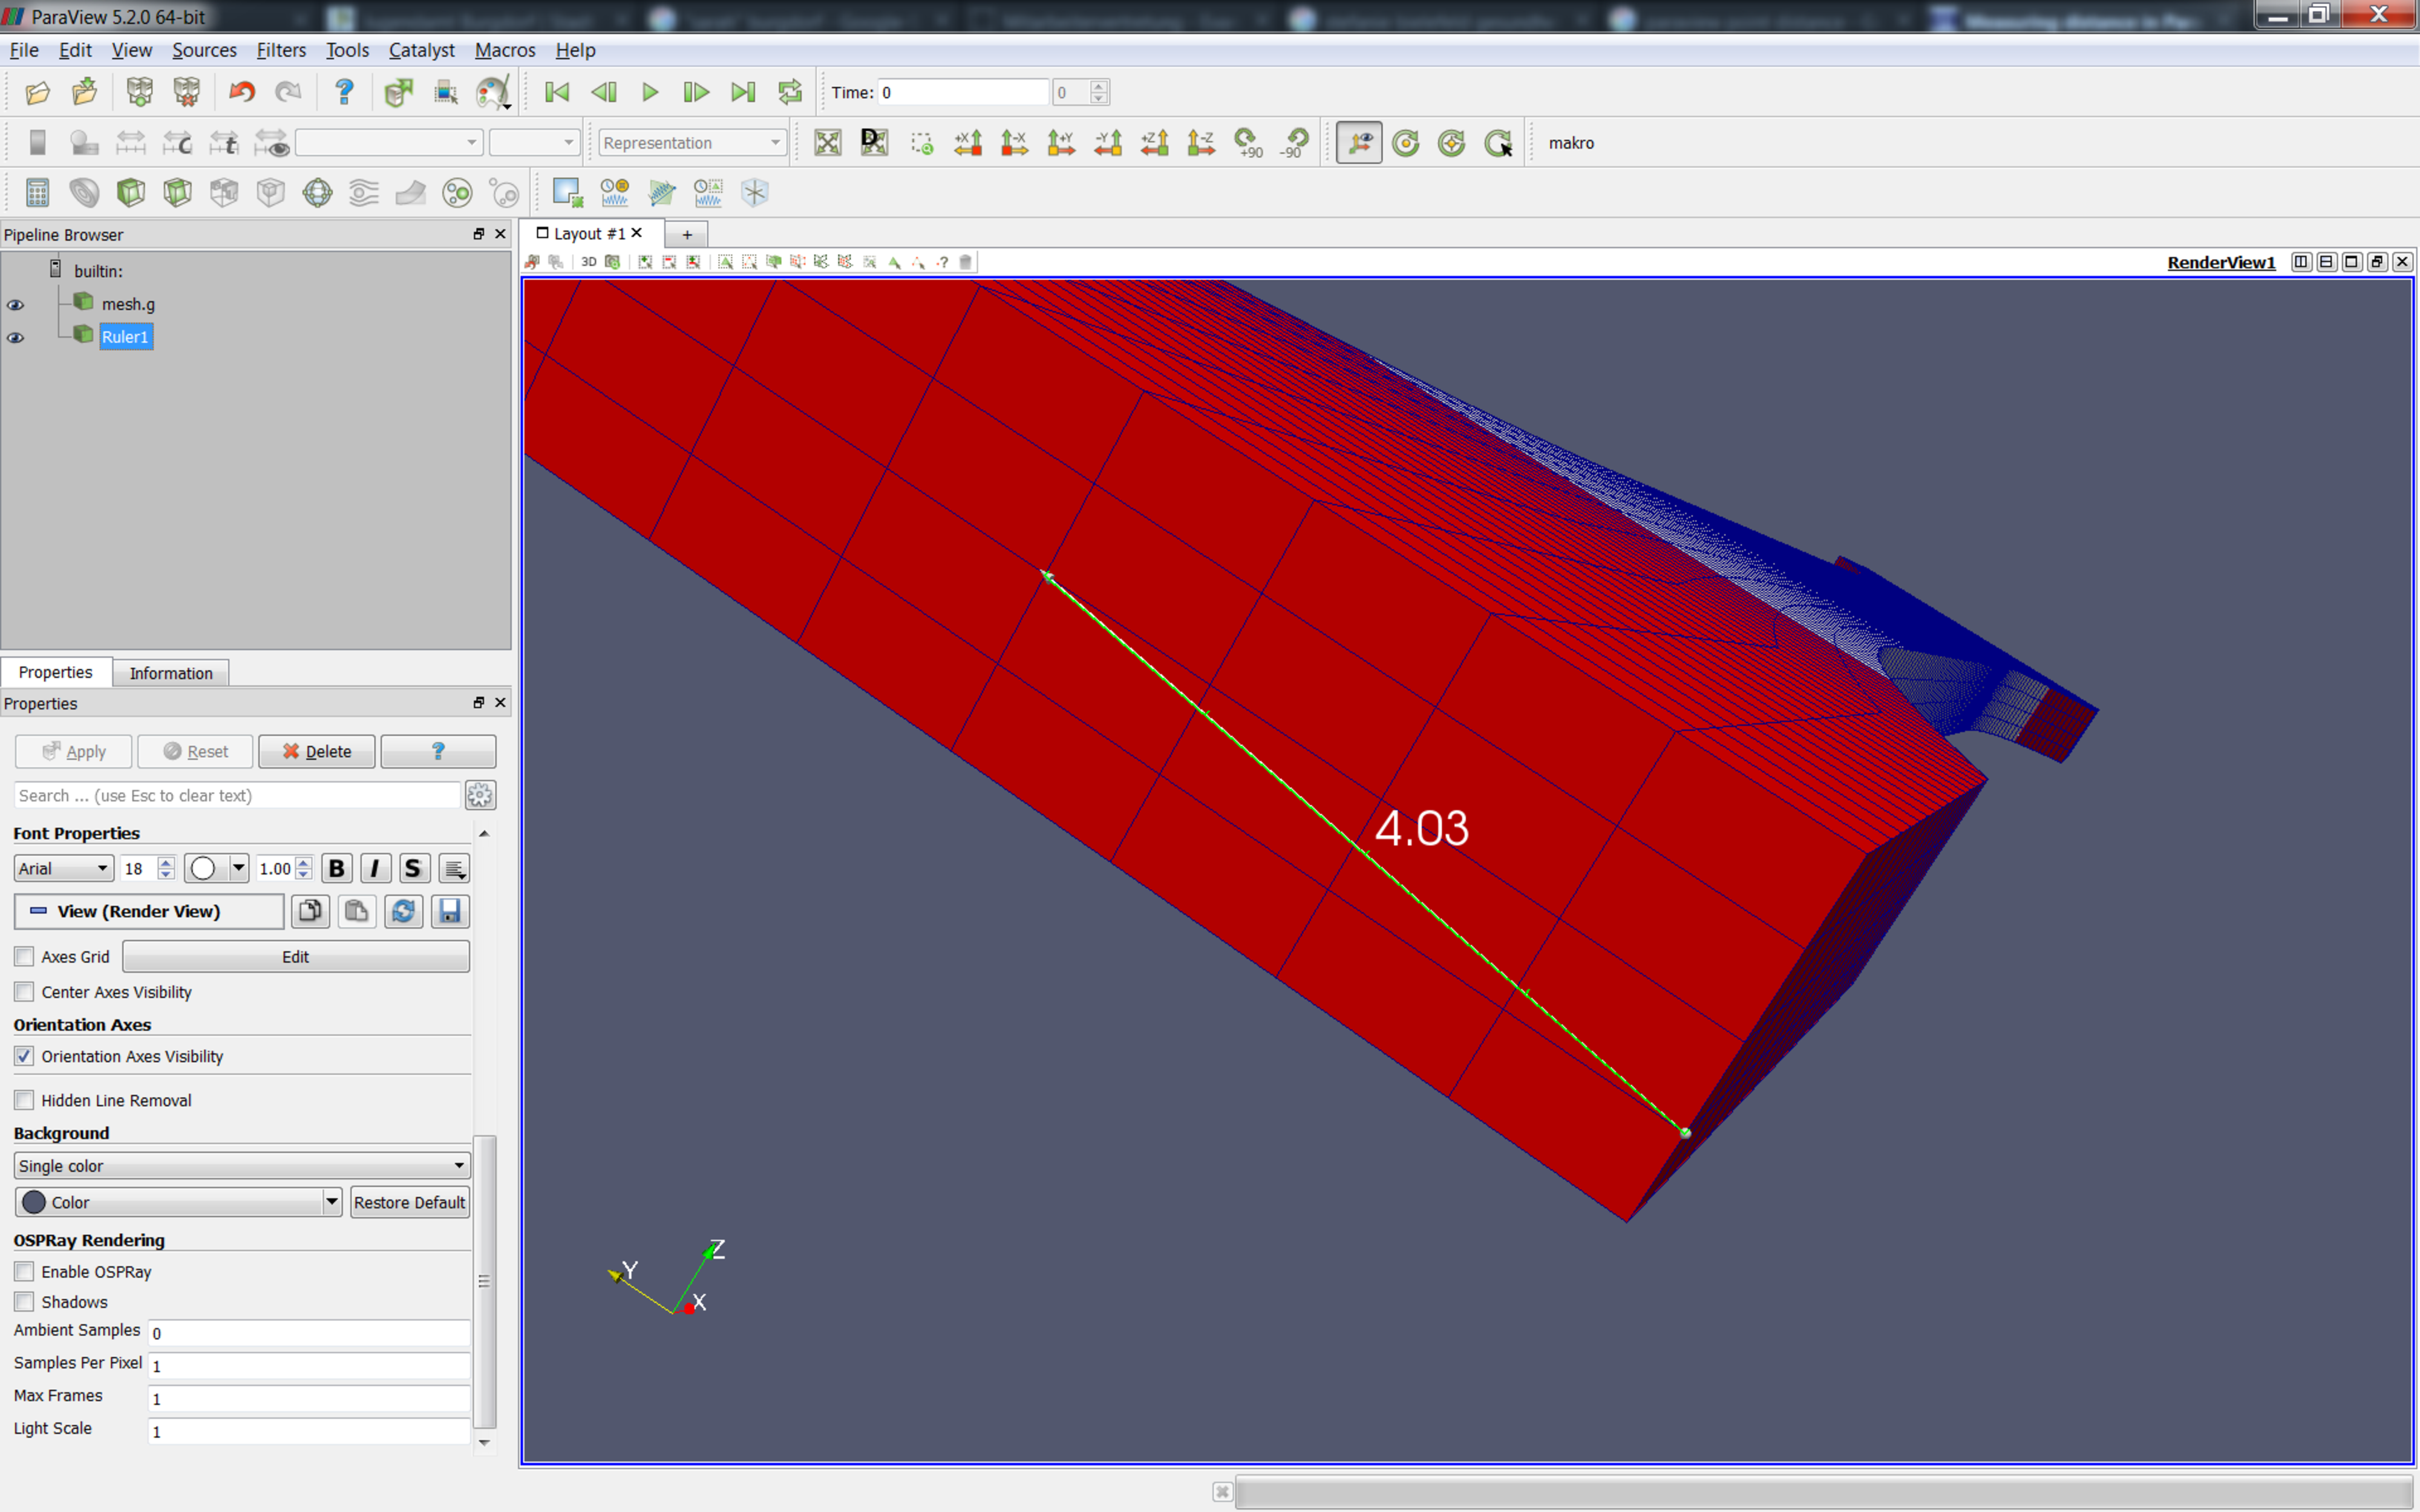
\includegraphics[width=\paraviewscreenshotwidthfac\linewidth]{Figures/Screenshots/ParaView_Measure_NodeDistance}};
    \begin{scope}[
      x={(image.south east)},
      y={(image.north west)},
    ]
      % Some label
%         \node[fit={(0.007,0.10) (0.18,0.17)},myrectangularmarkup] (rect1) {};
%         \node[anchor=west,mymarkuptext] (rect1label) at (rect1.east) {1};
%         %
%         \node[fit={(0.280,0.83) (0.31,0.86)},myrectangularmarkup] (rect2) {};
%         \node[anchor=west,mymarkuptext] (rect2label) at (rect2.east) {2};
      % Help grid and labels
%       \pic{myimagegrid};
    \end{scope}
  \end{tikzpicture}
\caption{Measure point distance in \protect\paraviewname}
\label{fig:Use_ParaView_Measure_NodeDistance}
\end{figure}

To measure the distance between two nodes or collocation points after importing the model:

\begin{enumerate}[noitemsep]
  \item In the menu bar
  \begin{itemize}[noitemsep]
    \item Click on \textit{Sources}
    \item Click \textit{Ruler}
  \end{itemize}
  \item In the render view
  \begin{itemize}[noitemsep]
    \item Left-click the first point and keep the mouse clicked
    \item Move the point close to the target
    \item Press ``CTRL+1'' and snap the point to the closest mesh point
    \item Do the same for the second point, but press ``CTRL+2'' instead for snapping
  \end{itemize}
  \item In the \textit{Ruler} properties window
  \begin{itemize}[noitemsep]
    \item Adjust preferences to your need
    \item Click \textit{Apply}
  \end{itemize}
  \item The number next to the \textit{Ruler} in the render view is the point distance
\end{enumerate}


\newpage
%%%%%%%%%%%%%%%%%%%%%%%%%%%%%%%%%%%%
% Header                           %
%%%%%%%%%%%%%%%%%%%%%%%%%%%%%%%%%%%%
% 
% Revisions: 2017-04-10 Martin R�del <martin.raedel@dlr.de>
%                       Initial draft
%               
% Contact:   Martin R�del,  martin.raedel@dlr.de
%            DLR Composite Structures and Adaptive Systems
%          
%                                 __/|__
%                                /_/_/_/  
%            www.dlr.de/fa/en      |/ DLR
% 
%%%%%%%%%%%%%%%%%%%%%%%%%%%%%%%%%%%%
% Content                          %
%%%%%%%%%%%%%%%%%%%%%%%%%%%%%%%%%%%%

\levelup{Exporting}
\leveldown{Quick Screenshot}

Screenshot are taken from the current view you see in \marktool{\paraviewname} render view. Therefore, perform all adjustments to the view to your needs before creating a screenshot.

To save a screenshot from \marktool{\paraviewname} perform the following steps:

\begin{enumerate}[noitemsep]
\item Click \textit{File} in the menubar
\item Click \textit{Save Screenshot}
\item Set plot preferences:
  \begin{itemize}[noitemsep]
  \item Uncheck \textit{Save only selected view} if necessary
  \item Activate the \textit{Lock aspect} button right of the resolution
  \item Change the resolution to values high enough for a print-quality picture\\(the higher value should at least be 1000)
  \item \textit{Select image quality} slider \tab 100
  \item Override color palette:	\tab \textit{Current palette}
  \item Stereo Mode:		\tab \textit{No stereo}
  \end{itemize}
\item Click \textit{Ok}
\item Specify the path and \textit{File name}
\item Choose \textit{PNG image} as file type
\item Click \textit{Ok}
\end{enumerate}

Afterwards, use \marktool{GIMP}, \marktool{Inkscape}, \marktool{convert} utility from \marktool{ImageMagick} or any other tool to convert the pixel to a non-scalable vector graphics copy as \verb+eps+ and \verb+pdf+ copy.

For the sake of reproducibility of the created picture save the \marktool{\paraviewname} state as described in section \ref{sec:Paraview_Save_States}.

The target must be to have the figure and the \marktool{\paraviewname} state file available at all time:

\begin{code}
figure_name.eps
figure_name.pdf
figure_name.png
figure_name.pvsm
\end{code}

\levelstay{Vector graphics - kind of}

The vector graphics output only affects the non-3D rendered elements such as texts, cube axes etc. Normal or glyph plots which are 3D rendered are not affected. Therefore, this option is currently no use for the documentation. It is proposed to create high-quality png-plot with the \textit{Save Screenshot} function and use \marktool{GIMP}, \marktool{Inkscape}, \marktool{convert} utility from \marktool{ImageMagick} or any other tool to convert the pixel to a non-scalable vector graphics copy.

\levelstay{Animations}	\label{sec:ParaView_Save_Animation}

\marktool{\paraviewname} allows the creation of animations for your currently selected view entity. So choose your plot coloring and vector entities before creating an animation.

To save an animation from \marktool{\paraviewname} perform the following steps:

\begin{enumerate}[noitemsep]
\item Click \textit{File} in the menubar
\item Click \textit{Save Animation}
\item Set animation preferences:
  \begin{itemize}[noitemsep]
  \item Animation duration:	\tab -
  \item Frame rate:		\tab $\ge$15	\\
  The human brain perceives successive images as moving, but not necessarily smooth, scene from about 14 to 16 frames per second.
  \item No. of Frames/timestep:	\tab 1
  \item Number of Frames:	\tab -
  \item Resolution:		\tab higher value $\ge$ 1000
  \item Timestep Range:		\tab Start- and end time step of interest
  \item Stereo Mode:		\tab \textit{No Stereo}
  \item Compression:		\tab Checked
  \end{itemize}
\item Click \textit{Save Animation}
\item Specify the path and \textit{File name}
\item Choose the file type of your liking, either video or multiple images
\item Click \textit{Ok}
\end{enumerate}

For the sake of reproducibility of the created animation save the \marktool{\paraviewname} state as described in section \ref{sec:Paraview_Save_States}.

The target must be to have the animation and the \marktool{\paraviewname} state file available at all time:

\begin{code}
animation_name.avi
animation_name.pvsm
\end{code}

\levelstay{Save \texorpdfstring{\protect\marktool{\paraviewname}}{\paraviewname{}} states for exported items}	\label{sec:Paraview_Save_States}

For the sake of reproducibility of the created picture or animation you can save the \marktool{\paraviewname} state. If you want to reproduce the picture or animation you can just load the state and all preferences will be set to the exact values of the saved state.

To save a state perform the following steps:

\begin{enumerate}[noitemsep]
\item Click \textit{File} in the menubar
\item Click \textit{Save State}
\item Specify the path of the figure or animation directory and the \textit{File name} identical to the figure file name
\item Choose \textit{ParaView state file (*.pvsm)} as file type
\item Click \textit{Ok}
\end{enumerate}

A state can be loaded accordingly:

\begin{enumerate}[noitemsep]
\item Click \textit{File} in the menubar
\item Click \textit{Load State}
\item Select the state file
\item Click \textit{Ok}
\end{enumerate}

\newpage
%%%%%%%%%%%%%%%%%%%%%%%%%%%%%%%%%%%%
% Header                           %
%%%%%%%%%%%%%%%%%%%%%%%%%%%%%%%%%%%%
% 
% Revisions: 2017-04-10 Martin R�del <martin.raedel@dlr.de>
%                       Initial draft
%               
% Contact:   Martin R�del,  martin.raedel@dlr.de
%            DLR Composite Structures and Adaptive Systems
%          
%                                 __/|__
%                                /_/_/_/  
%            www.dlr.de/fa/en      |/ DLR
% 
%%%%%%%%%%%%%%%%%%%%%%%%%%%%%%%%%%%%
% Content                          %
%%%%%%%%%%%%%%%%%%%%%%%%%%%%%%%%%%%%

\levelup{Preferences}

\leveldown{Change mesh on sphere \texttt{Glyph}}

Sometimes for nice publication pictures the default sphere glyph representation might be a little too angular. Internally, sphere glyphs are nothing but a combination of a certain number of tetrahedron elements. Thus, the mesh behind a sphere glyph might be too coarse. It is assumed you already have a glyph as spheres, otherwise have a look at \autoref{sec:ParaView_Damage_Plots_on_Nodes_as_Spheres}. 

In order to change the mesh size and smooth the sphere shape perform the following steps:

\begin{enumerate}[noitemsep]
\item Select the Glyph in the \textit{Pipeline Browser}
\item In the \textit{Properties} tab
  \begin{itemize}[noitemsep]
  \item Below the top line press the gear symbol 
\includegraphics[width=\iconsize]{Figures/Icons/pqAdvanced26}
  \item Additional options in section \textit{Glyph Source} appear
  \item Adjust the values for \textit{Theta resolution} and \textit{Phi resolution} to your needs. The default coarse value is 8.
  \item Click 
\includegraphics[width=\iconsize]{Figures/Icons/pqAutoApply32} \textit{Apply}
  \end{itemize}
\end{enumerate}

The result is compared in \autoref{fig:ParaView_Glyph_Mesh}. The mesh refinement has a significant impact on the computational performance. So only use the refined mesh if it is really necessary.

\begin{figure}[htbp]
  \begin{subfigure}{0.49\linewidth}
    \centering
    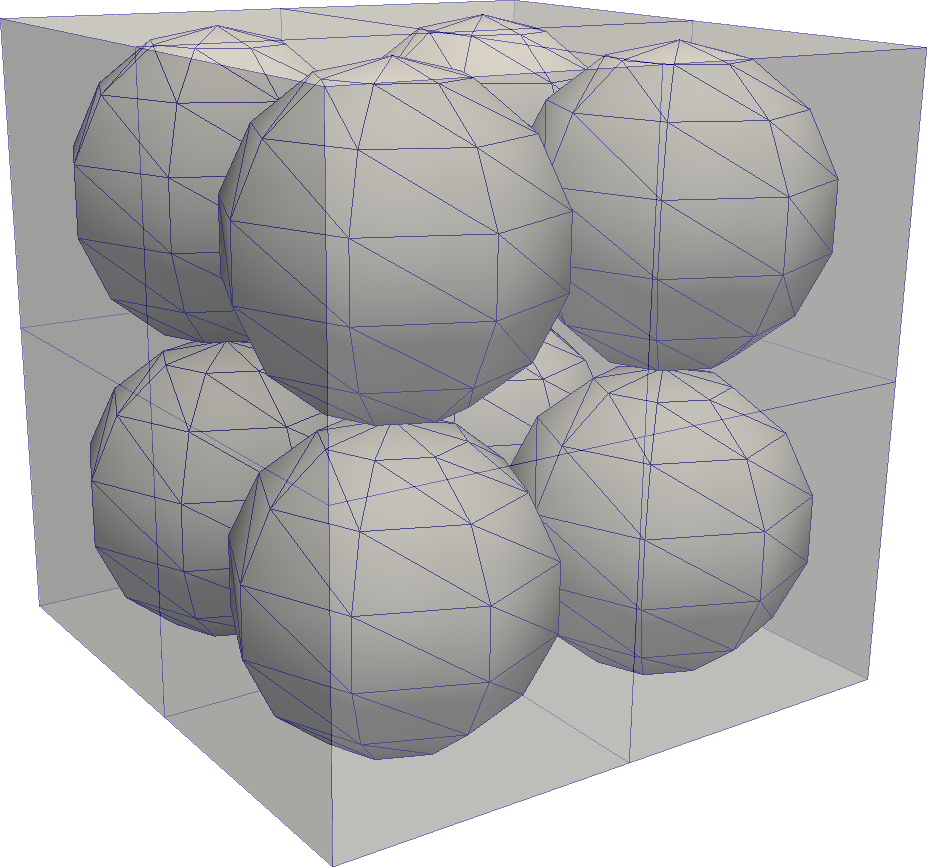
\includegraphics[width=0.85\linewidth]{Figures/ParaView/ParaView_Glyph_Mesh8}
    \caption{Resolution=8}
    \label{fig:ParaView_Glyph_Mesh8}
  \end{subfigure}%
  \begin{subfigure}{0.49\linewidth}
    \centering
    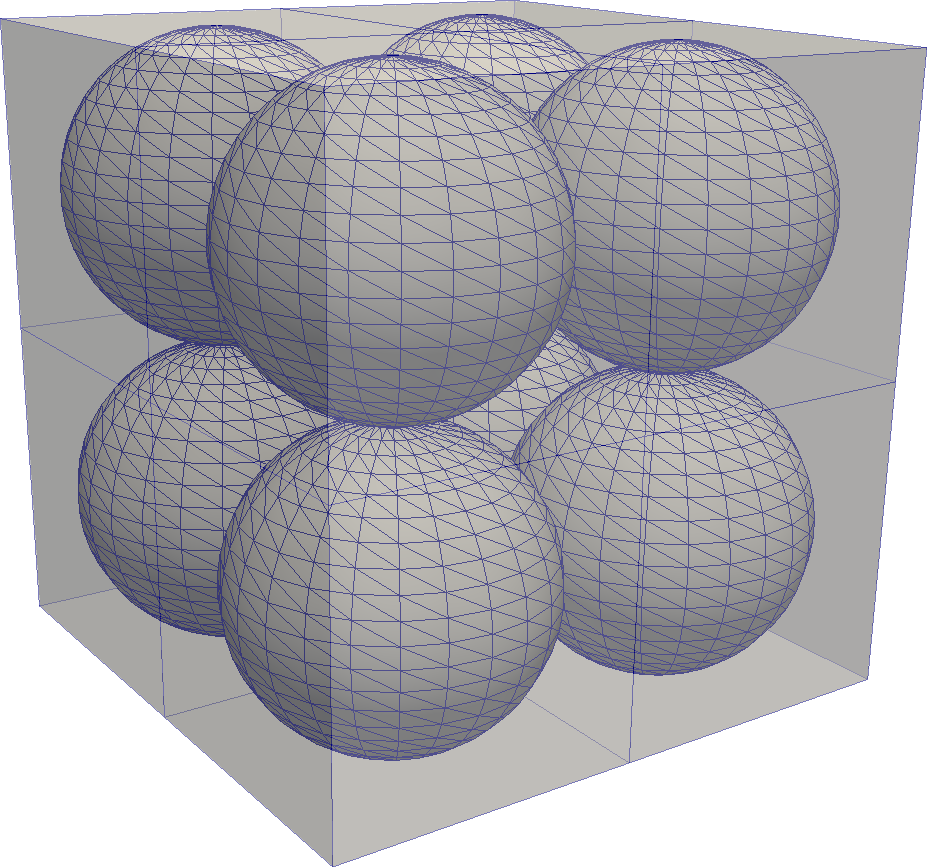
\includegraphics[width=0.85\linewidth]{Figures/ParaView/ParaView_Glyph_Mesh24}
    \caption{Resolution=24}
    \label{fig:ParaView_Glyph_Mesh24}
  \end{subfigure}%
  \caption{\protect\marktool{\toolname} collocation points inside the base finite element mesh with different glyph resolutions}
  \label{fig:ParaView_Glyph_Mesh}
\end{figure}



\newpage
%%%%%%%%%%%%%%%%%%%%%%%%%%%%%%%%%%%%
% Header                           %
%%%%%%%%%%%%%%%%%%%%%%%%%%%%%%%%%%%%
% 
% Revisions: 2017-04-10 Martin R�del <martin.raedel@dlr.de>
%                       Initial draft
%               
% Contact:   Martin R�del,  martin.raedel@dlr.de
%            DLR Composite Structures and Adaptive Systems
%          
%                                 __/|__
%                                /_/_/_/  
%            www.dlr.de/fa/en      |/ DLR
% 
%%%%%%%%%%%%%%%%%%%%%%%%%%%%%%%%%%%%
% Content                          %
%%%%%%%%%%%%%%%%%%%%%%%%%%%%%%%%%%%%

\levelup{Calculate}

%%%%%%%%%%%%%%%%%%%%%%%%%%%%%%%%%%%%
% Header                           %
%%%%%%%%%%%%%%%%%%%%%%%%%%%%%%%%%%%%
% 
% Revisions: 2017-04-10 Martin R�del <martin.raedel@dlr.de>
%                       Initial draft
%               
% Contact:   Martin R�del,  martin.raedel@dlr.de
%            DLR Composite Structures and Adaptive Systems
%          
%                                 __/|__
%                                /_/_/_/  
%            www.dlr.de/fa/en      |/ DLR
% 
%%%%%%%%%%%%%%%%%%%%%%%%%%%%%%%%%%%%
% Content                          %
%%%%%%%%%%%%%%%%%%%%%%%%%%%%%%%%%%%%

\leveldown{Cell center}
\label{sec:ParaView:Calculate:Cell:Center}

\begin{enumerate}[noitemsep]
\item Import your model and create a selection if only specific cell volumes are of interest.
\item Select the model or selection in the \textit{Pipeline Browser}
\item From the menu bar:
  \begin{itemize}[noitemsep]
  \item Click Filters
  \item Click Alphabetical
  \item Click \textit{Cell centers}
  \end{itemize}
\item In the \textit{Properties} tab
  \begin{itemize}[noitemsep]
    \item Select all blocks of interest in the \textit{Composite Data Set Index}
  \end{itemize}
\item Click \textit{Apply}
\item Open a new \textit{Spreadsheet View}
\item In the \textit{Showing} combobox select your \textit{Cell Center Filter Name} and \textit{Point Data} in the \textit{Attribute} combobox
\item Column \textit{points} shows the cell center
\end{enumerate}
%%%%%%%%%%%%%%%%%%%%%%%%%%%%%%%%%%%%
% Header                           %
%%%%%%%%%%%%%%%%%%%%%%%%%%%%%%%%%%%%
% 
% Revisions: 2017-04-10 Martin R�del <martin.raedel@dlr.de>
%                       Initial draft
%               
% Contact:   Martin R�del,  martin.raedel@dlr.de
%            DLR Composite Structures and Adaptive Systems
%          
%                                 __/|__
%                                /_/_/_/  
%            www.dlr.de/fa/en      |/ DLR
% 
%%%%%%%%%%%%%%%%%%%%%%%%%%%%%%%%%%%%
% Content                          %
%%%%%%%%%%%%%%%%%%%%%%%%%%%%%%%%%%%%

\levelstay{Cell volume}
\label{sec:ParaView:Calculate:Cell:Volume}

A method is described that allows the calculation/extraction of the cell or element volume. This solution is copied from the \href{https://public.kitware.com/pipermail/paraview/2015-October/035367.html}{Paraview Mailing List}.

\begin{enumerate}[noitemsep]
\item Import your model and create a selection if only specific cell volumes are of interest.
\item Select the model or selection in the \textit{Pipeline Browser}
\item From the menu bar:
  \begin{itemize}[noitemsep]
  \item Click Filters
  \item Click Data Analysis
  \item Click \textit{Programmable Filter}
  \end{itemize}
\item In the \textit{Properties} tab
  \begin{itemize}[noitemsep]
    \item Add to the \textit{Script} field:
\begin{code}
from vtk.numpy_interface import algorithms as algs

volume = algs.volume(inputs[0])
output.CellData.append(volume, 'volume')
\end{code}
    \item Select all blocks of interest in the \textit{Composite Data Set Index}
  \end{itemize}
\item Click \textit{Apply}
\item Open a new \textit{Spreadsheet View}
\item In the \textit{Showing} combobox select your \textit{Programmable Filter} and \textit{Cell Data} in the \textit{Attribute} combobox
\item Column \textit{volume} shows the cell volume
\end{enumerate}

\begin{figure}[htbp]
\centering
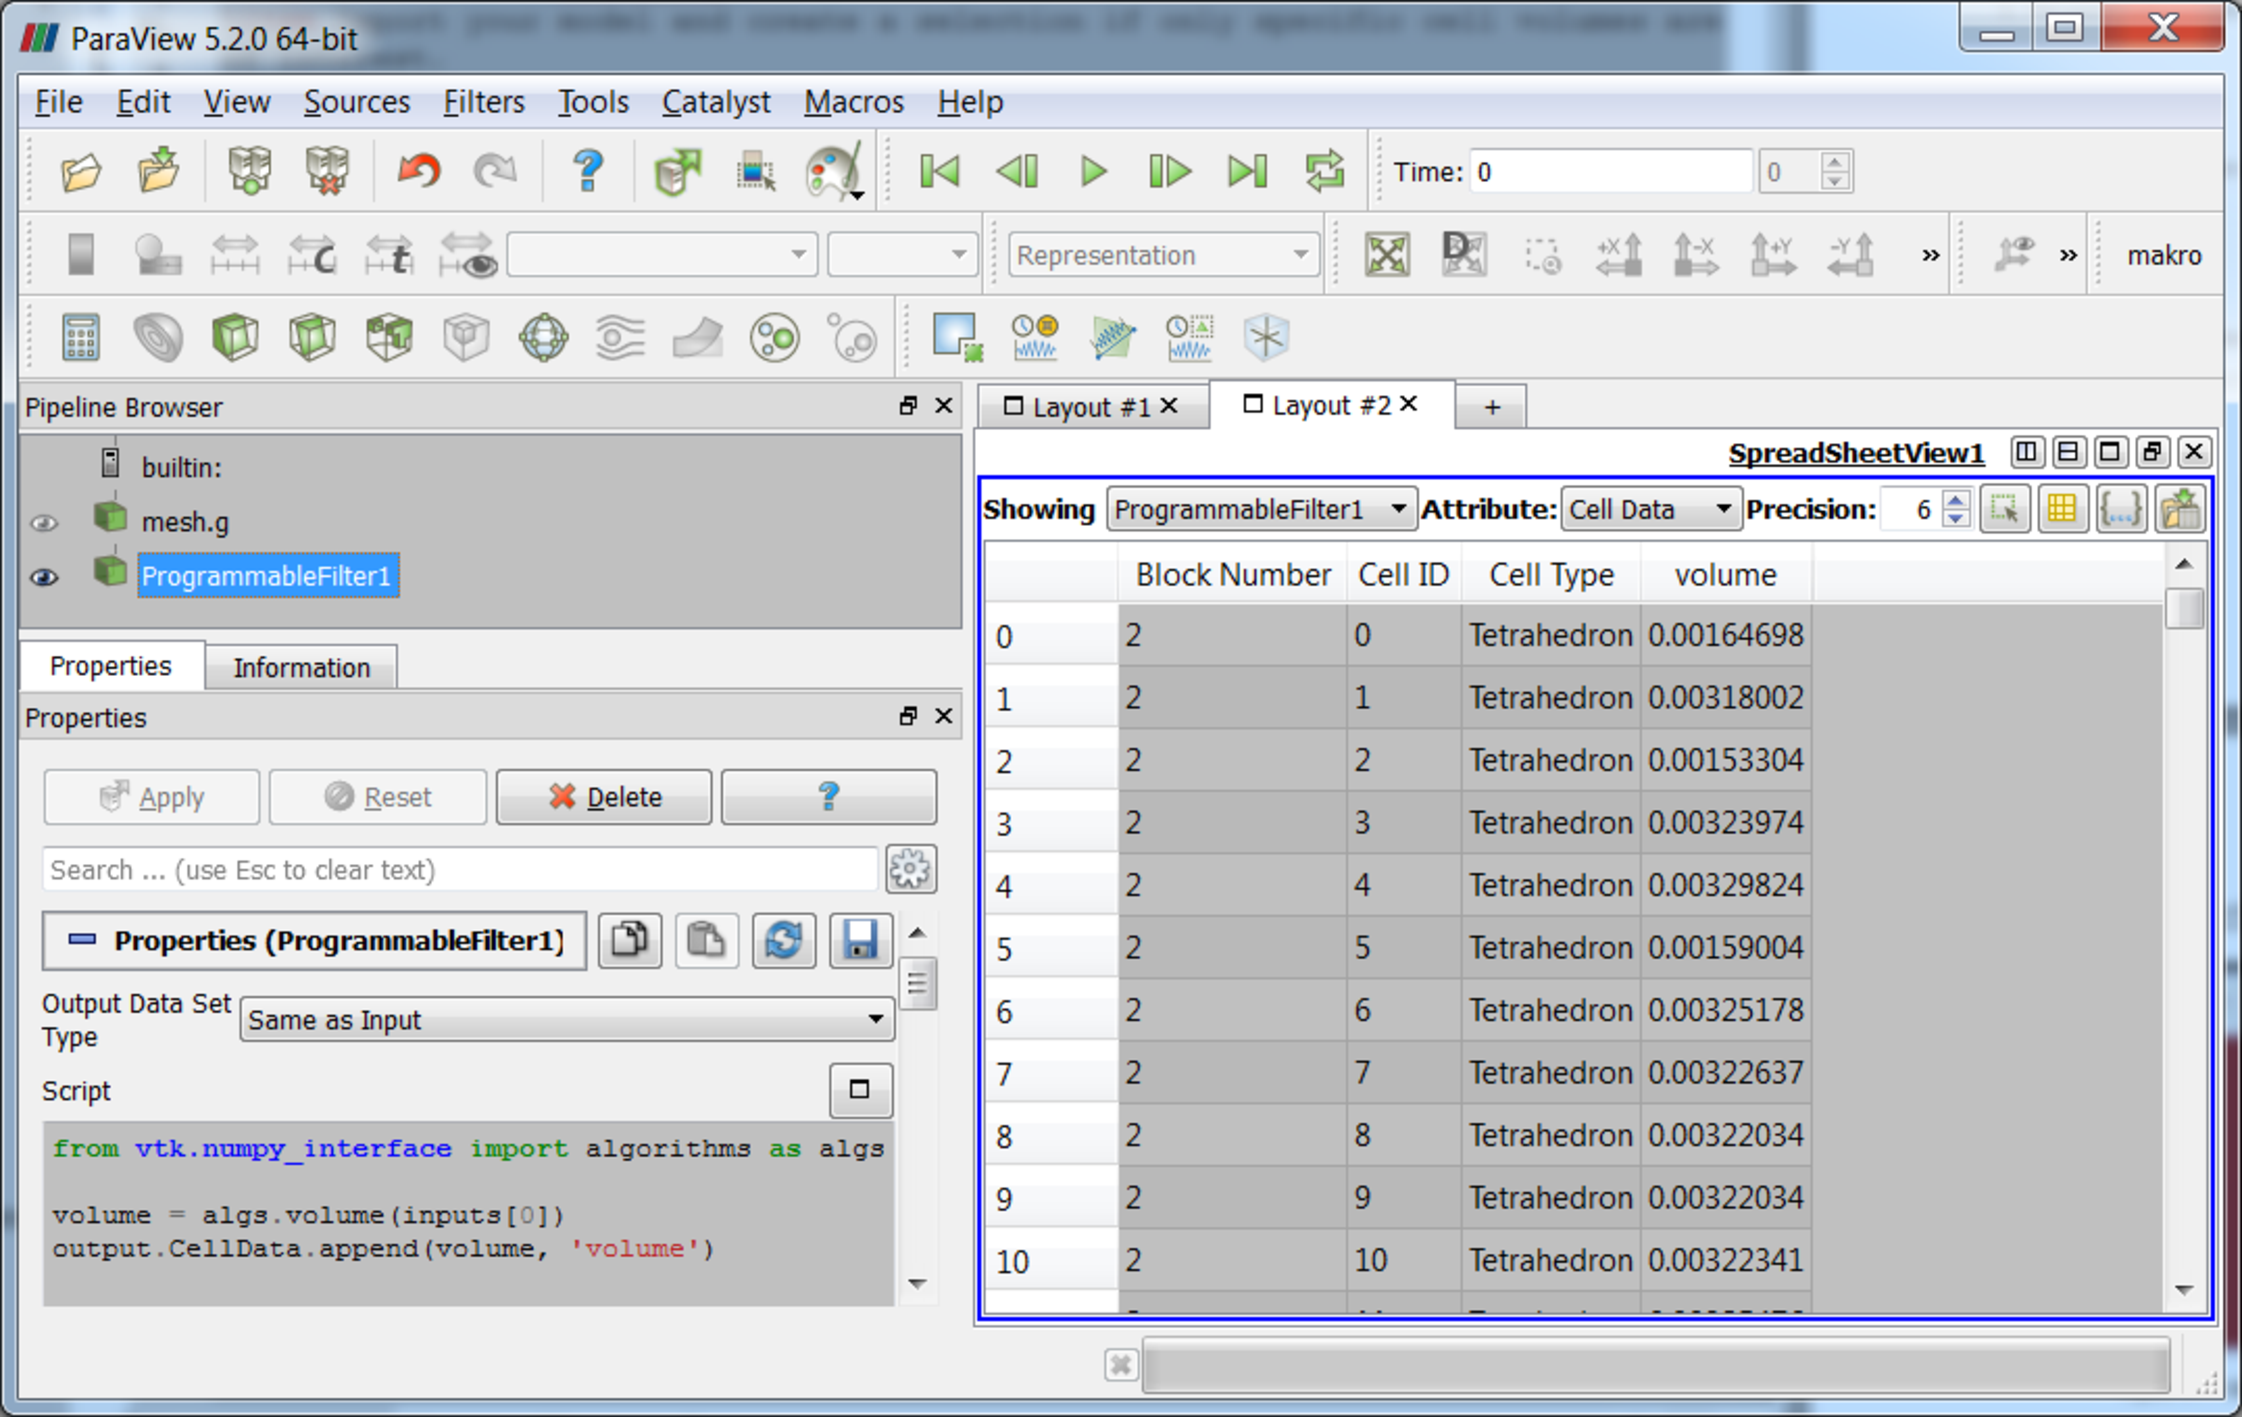
\includegraphics[width=\paraviewscreenshotwidthfac\linewidth]{Figures/Screenshots/ParaView_Calculate_Cell_Volume}
\caption{Display of cell volume calculation}
\label{fig:ParaView:Calculate:Cell:Volume}
\end{figure}

%%%%%%%%%%%%%%%%%%%%%%%%%%%%%%%%%%%%
% Header                           %
%%%%%%%%%%%%%%%%%%%%%%%%%%%%%%%%%%%%
% 
% Revisions: 2017-04-10 Martin R�del <martin.raedel@dlr.de>
%                       Initial draft
%               
% Contact:   Martin R�del,  martin.raedel@dlr.de
%            DLR Composite Structures and Adaptive Systems
%          
%                                 __/|__
%                                /_/_/_/  
%            www.dlr.de/fa/en      |/ DLR
% 
%%%%%%%%%%%%%%%%%%%%%%%%%%%%%%%%%%%%
% Content                          %
%%%%%%%%%%%%%%%%%%%%%%%%%%%%%%%%%%%%

\chapter{Benchmark results with \texorpdfstring{\protect\marktool{\toolnameshort}}{\toolnameshort{}}}
\setcounter{currentlevel}{6}

\marktool{\toolname} comes with several example problems as well as unit-test models which can be found in the following directories of the \marktool{\toolname} installation folder.

\begin{itemize}[noitemsep]
  \item \texttt{/examples/}
  \item \texttt{/test/}
\end{itemize}

Further examples are available and documented in the \marktool{\toolname} Models and Verification Guide which is part of the same repository.


%%%%%%%%%%%%%%%%%%%%%%%%%%%%%%%%%%%%
% Bibliography                     %
%%%%%%%%%%%%%%%%%%%%%%%%%%%%%%%%%%%%

\printbibliography

%%%%%%%%%%%%%%%%%%%%%%%%%%%%%%%%%%%%
% Index                            %
%%%%%%%%%%%%%%%%%%%%%%%%%%%%%%%%%%%%

\printindex[\idxPDKeywordName]

%%%%%%%%%%%%%%%%%%%%%%%%%%%%%%%%%%%%
% Appendix                         %
%%%%%%%%%%%%%%%%%%%%%%%%%%%%%%%%%%%%

%%%%%%%%%%%%%%%%%%%%%%%%%%%%%%%%%%%%
% Header                           %
%%%%%%%%%%%%%%%%%%%%%%%%%%%%%%%%%%%%
% 
% Revisions: 2017-04-10 Martin Rädel <martin.raedel@dlr.de>
%                       Initial draft
%               
% Contact:   Martin Rädel,  martin.raedel@dlr.de
%            DLR Composite Structures and Adaptive Systems
%          
%                                 __/|__
%                                /_/_/_/  
%            www.dlr.de/fa/en      |/ DLR
% 
%%%%%%%%%%%%%%%%%%%%%%%%%%%%%%%%%%%%
% Content                          %
%%%%%%%%%%%%%%%%%%%%%%%%%%%%%%%%%%%%

\begin{appendices}

\chapter{Build-scripts for Libraries}
\setcounter{currentlevel}{6}
%%%%%%%%%%%%%%%%%%%%%%%%%%%%%%%%%%%%
% Header                           %
%%%%%%%%%%%%%%%%%%%%%%%%%%%%%%%%%%%%
% 
% Revisions: 2017-04-10 Martin Rädel <martin.raedel@dlr.de>
%                       Initial draft
%               
% Contact:   Martin Rädel,  martin.raedel@dlr.de
%            DLR Composite Structures and Adaptive Systems
%          
%                                 __/|__
%                                /_/_/_/  
%            www.dlr.de/fa/en      |/ DLR
% 
%%%%%%%%%%%%%%%%%%%%%%%%%%%%%%%%%%%%
% Content                          %
%%%%%%%%%%%%%%%%%%%%%%%%%%%%%%%%%%%%

In the following sections, the build scripts for the libraries for \marktool{\toolname} are collected. These are Bash-scripts or \marktool{\cmakename}-files.

The scripts are taken from \href{https://peridigm.sandia.gov/}{https://peridigm.sandia.gov/} and modified slightly if necessary.

The files are provided with UTF-8 encoding. Please modify to your needs if necessary.

\leveldown{\texorpdfstring{\protect\marktool{\boostname{}}}{\boostname{}}}
\label{sec:Build-script_Boost}

\leveldown{\texorpdfstring{\protect\marktool{\boostname{}}}{\boostname{}} 1.55.0}

Open a text editor, copy the following code into a file and save as \verb+install_boost-1.55.0.sh+

\begingroup
\lstset{breaklines = true}
\lstinputlisting[
  style=scriptstyle,
  caption=Install script for \protect\marktool{\boostname} 1.55.0,
  label=lst:install_boost
]{Scripts/install_boost-1.55.0.sh}
\endgroup

\ifpdf
Alternatively, you can \textattachfile[author=raed_ma, color=0 0 1]{Scripts/install_boost-1.55.0.sh}{download} the script from within this document.
\fi

\levelstay{\texorpdfstring{\protect\marktool{\boostname{}}}{\boostname{}} 1.60.0}

Open a text editor, copy the following code into a file and save as \verb+install_boost-1.60.0.sh+

\begingroup
\lstset{breaklines = true}
\lstinputlisting[
  style=scriptstyle,
  caption=Install script for \protect\marktool{\boostname} 1.60.0,
  label=lst:install_boost-1.60.0
]{Scripts/install_boost-1.60.0.sh}
\endgroup

\ifpdf
Alternatively, you can \textattachfile[author=raed_ma, color=0 0 1]{Scripts/install_boost-1.60.0.sh}{download} the script from within this document.
\fi

\levelup{\texorpdfstring{\protect\marktool{\hdfname{}}}{\hdfname{}}}
\label{sec:Build-script_HDF}

Open a text editor, copy the following code into a file and save as \verb+install_hdf.sh+

\begingroup
\lstset{breaklines = true}
\lstinputlisting[
  style=scriptstyle,
  caption=Install script for \protect\marktool{\hdfname},
  label=lst:install_hdf
]{Scripts/install_hdf.sh}
\endgroup

\ifpdf
Alternatively, you can \textattachfile[author=raed_ma, color=0 0 1]{Scripts/install_hdf.sh}{download} the script from within this document.
\fi

\levelstay{\texorpdfstring{\protect\marktool{\netcdfname{}}}{\netcdfname{}}}
\label{sec:Build-script_NetCDF}

Open a text editor, copy the following code into a file and save as \verb+install_netcdf.sh+

\begingroup
\lstset{breaklines = true}
\lstinputlisting[
  style=scriptstyle,
  caption=Install script for \protect\marktool{\netcdfname},
  label=lst:install_netcdf
]{Scripts/install_netcdf.sh}
\endgroup

\ifpdf
Alternatively, you can \textattachfile[author=raed_ma, color=0 0 1]{Scripts/install_netcdf.sh}{download} the script from within this document.
\fi

% Other proposal from \href{http://diehlpk.github.io/2015/06/22/builing-peridigm.html}{http://diehlpk.github.io/2015/06/22/builing-peridigm.html}
% 
% \begin{code}
% # Set environment variables for MPI compilers
% export CC=mpicc
% export CXX=mpicxx
% export FC=mpif90
% export F77=mpif77
% 
% # 
% H5DIR=/usr/local/hdf5/ \
% export CPPFLAGS="-I${H5DIR}/include" \
% export LDFLAGS=-L${H5DIR}/lib \
% 
% # Configure NetCDF \
% CPPFLAGS="-I${H5DIR}/include" LDFLAGS=-L${H5DIR}/lib  ../configure --prefix=/usr/local/netcdf/  --disable-netcdf-4 --disable-dap --enable-parallel \
% 
% # Make, test, and install NetCDF
% make -j 8
% make check
% make install
% \end{code}

\levelstay{\texorpdfstring{\protect\marktool{\trilinosname{}}}{\trilinosname{}}}
\label{sec:Build-script_Trilinos}

Open an editor, copy the following code into the file and save as \verb+cmake_trilinos.cmake+. The final line marks the path to the \marktool{\trilinosname} source directory, which is named \verb+$DOWNLOAD_DIR+ in the documentation.

\begingroup
\lstset{breaklines = true}
\lstinputlisting[
  style=scriptstyle,
  caption=\protect\marktool{\cmakename} script for \protect\marktool{\trilinosname},
  label=lst:cmake_trilinos
]{Scripts/cmake_trilinos.cmake}
\endgroup

\ifpdf
Alternatively, you can \textattachfile[author=raed_ma, color=0 0 1]{Scripts/cmake_trilinos.cmake}{download} the script from within this document.
\fi

\levelstay{\texorpdfstring{\protect\marktool{\toolname{}}}{\toolname{}}}
\label{sec:Build-script_Peridigm}

\leveldown{\texorpdfstring{\protect\marktool{\cmakename{}}}{\cmakename{}} script for \texorpdfstring{\protect\marktool{\toolnameshort{}}}{\toolnameshort{}}}
\label{sec:Build-script_Peridigm:cmake}

Open an editor, copy the following code into the file and save as \verb+cmake_peridigm.cmake+. The final line marks the path to the \marktool{\toolname} source directory, which is named \verb+$DOWNLOAD_DIR+ in the documentation.

\begingroup
\lstset{breaklines = true}
\lstinputlisting[
  style=scriptstyle,
  caption=\protect\marktool{\cmakename} script for \protect\marktool{\toolnameshort},
  label=lst:cmake_peridigm
  ]{Scripts/cmake_peridigm.cmake}
\endgroup

\ifpdf
Alternatively, you can \textattachfile[author=raed_ma, color=0 0 1]{Scripts/cmake_peridigm.cmake}{download} the script from within this document.
\fi

\levelstay{Script for cloning \texorpdfstring{\protect\marktool{\toolnameshort{}}}{\toolnameshort{}} from GitHub and compiling on the STM-Cluster}
\label{sec:Build-script_Peridigm:Cluster}

\begingroup
\lstset{breaklines = true}
\lstinputlisting[
  style=scriptstyle,
  caption=Script for cloning \protect\marktool{\toolnameshort} from GitHub and compiling on the STM-Cluster,
  label=lst:shell_peridigm
  ]{Scripts/install_peridigm_github.sh}
\endgroup

\ifpdf
Alternatively, you can \textattachfile[author=raed_ma, color=0 0 1]{Scripts/install_peridigm_github.sh}{download} the script from within this document.
\fi

\levelup{Make a script executable}	\label{sec:Build-script_Executable}

In order to use a script file in the shell for installation you must first make the text file executable. Therefore, open a terminal, change directory to the folder the individual script is located and make the script executable for the user with

\begin{code}
chmod u+x $SCRIPTNAME.sh
\end{code}

\levelstay{Modifications of \texttt{.bashrc}}	\label{sec:Build-script_Bashrc}

When an interactive shell that is not a login shell is started, bash reads and executes commands from \verb+~/.bashrc+, if that file exists. You can find the \verb+.bashrc+ file in your user home directory \verb+/home/$USER/+ with \verb+ls -al+.

The following listings shows a modified \verb+.bashrc+ file which includes the exportation of the significant libraries in the \verb+$PATH+ and \verb+$LD_LIBRARY_PATH+ environment variables. The header is not printed.

\textbf{Be aware}:

\begin{itemize}[noitemsep]
 \item In case you use a 32bit operating system, or in some cases also for 64bit operating system, the lib64-folders must be changed to lib.
 \item The entries to the \verb+$PATH+ and \verb+$LD_LIBRARY_PATH+ variables should be added step-by-step \textbf{after} the installation of the individual tool. Otherwise, the install scripts might find pre-compiled items and use these instead of creating new binaries with the current settings.
\end{itemize}

\leveldown{\texttt{.bashrc} for \texorpdfstring{\protect\marktool{\toolnameshort{}}}{\toolnameshort{}} 1.4.1}

\begingroup
\lstset{breaklines = true}
\lstinputlisting[
  style=scriptstyle,
  firstline=28,
  caption=Modified .bashrc-file to set environment variables for \marktool{\toolname} 1.4.1,
  label=lst:bashrc_mod_1.4.1
]{Scripts/modified_bashrc.txt}
\endgroup

\ifpdf
You can \textattachfile[author=raed_ma, color=0 0 1]{Scripts/modified_bashrc.txt}{download} the file from within this document.
\fi

\levelstay{\texttt{.bashrc} for \texorpdfstring{\protect\marktool{\toolnameshort{}}}{\toolnameshort{}} 1.5}

\begingroup
\lstset{breaklines = true}
\lstinputlisting[
  style=scriptstyle,
  firstline=28,
  caption=Modified .bashrc-file to set environment variables for \marktool{\toolname} 1.5,
  label=lst:bashrc_mod_1.5
]{Scripts/modified_bashrc_Peridigm_1.5.txt}
\endgroup

\ifpdf
You can \textattachfile[author=raed_ma, color=0 0 1]{Scripts/modified_bashrc_Peridigm_1.5.txt}{download} the file from within this document.
\fi

\chapter{FAQ}
\setcounter{currentlevel}{6}
%%%%%%%%%%%%%%%%%%%%%%%%%%%%%%%%%%%%
% Header                           %
%%%%%%%%%%%%%%%%%%%%%%%%%%%%%%%%%%%%
% 
% Revisions: 2017-04-10 Martin R�del <martin.raedel@dlr.de>
%                       Initial draft
%               
% Contact:   Martin R�del,  martin.raedel@dlr.de
%            DLR Composite Structures and Adaptive Systems
%          
%                                 __/|__
%                                /_/_/_/  
%            www.dlr.de/fa/en      |/ DLR
%
%%%%%%%%%%%%%%%%%%%%%%%%%%%%%%%%%%%%
% Content                          %
%%%%%%%%%%%%%%%%%%%%%%%%%%%%%%%%%%%%

\chapter{FAQ}
\setcounter{currentlevel}{6}

\leveldown{\protect\toolname{}}

\begin{description}[leftmargin=\parindent,labelindent=\parindent,style=nextline]
% 
\item[When I call \marktool{\toolname} with \texttt{mpirun} I get an error that the program is unable to find the mesh file. What can I do? ]\mbox{}\\[-2.5\baselineskip]
  \begin{itemize}[noitemsep]
  \item This problem occurs for \marktool{\cubitname} mesh files (*.g)
  \item Before using them in a parallel job you have to decompose the mesh according to the number of processors to be used
  \item Please consult section \ref{sec:Peridigm:Run:Execution:Local:Input}
  \end{itemize}
%
\item[Everything works fine but when I call \marktool{decomp} I get a \texttt{***HDF5 library version mismatched error***} error. Why? ]\mbox{}\\[-2.5\baselineskip]
  \begin{itemize}[noitemsep]
  \item Check this same question in the \marktool{\toolname} Installation Guide from this same repository.
  \end{itemize}
%
\item[I get the following error message combination: \texttt{Throw test that evaluated to true: !boost::math::isfinite((*force)[i])} and \texttt{**** NaN returned by force evaluation.}. Why?]\mbox{}\\[-2.5\baselineskip]
  \begin{itemize}[noitemsep]
%   \item There seems to be no body load or non-zero kinematic boundary condition in your model.
%   \item See if the definition of \texttt{Body load} or \texttt{Prescribed Displacement} is working correctly in your model.
    \item It may be that your model became numerically unstable. Try to calculate the model again with a decreased value for the solver timestep safety factor.
  \end{itemize}
%
\item[I get the following error message: \texttt{**** Error:  getFieldId(), label not found:  Force} when using a \texttt{Compute Class Parameters}. Why?]\mbox{}\\[-2.5\baselineskip]
  \begin{itemize}[noitemsep]
    \item Make sure you request the \texttt{Variable} as a normal \texttt{Output Variable} as well. Have a look at the remarks in sections \ref{sec:Peridigm:QRG:ComputeClassParameters:Nodeset:Parameters}, \ref{sec:Peridigm:QRG:ComputeClassParameters:Block:Parameters} \& \ref{sec:Peridigm:QRG:ComputeClassParameters:NearestPoint:Parameters}.
    \item E.g. if your \texttt{Compute Class Parameter} is a force, \texttt{Force} must also be specified in the output section
  \end{itemize}
%
\item[I get the following error message: \texttt{Error!  An attempt was made to access parameter "ABC" of type "int" in the parameter (sub)list "ANONYMOUS"
using the incorrect type "double"!} in when using the function parser for an input parameter. Why?]\mbox{}\\[-2.5\baselineskip]
  \begin{itemize}[noitemsep]
    \item Make sure that the equation for the function parser does not result in a numerical value that can be expressed as an integer. E.g. With the values  \lstinline[style=inlinecodestyle]+#{DISPLACEMENT=1.0}+ and \lstinline[style=inlinecodestyle]+#{VELOCITY=1.0}+ the \texttt{Final Time} of a solver \lstinline[style=inlinecodestyle]+Final Time {DISPLACEMENT/VELOCITY}+ supposedly is 1.0. However, for the function parser the result is 1 as an integer. As a double value is expected for \texttt{Final Time} an error is thrown.
  \end{itemize}
%
\item[I get the following error message: \texttt{Error, the parameter "ABC" is not a list, it is of type "double"!} using the free format (.peridigm model). Why?]\mbox{}\\[-2.5\baselineskip]
  \begin{itemize}[noitemsep]
    \item Make sure there are no tabs in the line of ``ABS''. If there are, replace them with spaces and adjust the indentation of the line to the free format in your model.
  \end{itemize}
%
\item[Nothing happens when I use the \texttt{Implicit} solver and time-dependent \texttt{Prescribed Displacement}s. Why?]\mbox{}\\[-2.5\baselineskip]
  \begin{itemize}[noitemsep]
    \item This seems to be a bug in the calculation of the forces.
    \item See \href{https://github.com/peridigm/peridigm/issues/23}{https://github.com/peridigm/peridigm/issues/23}
  \end{itemize}
%
\end{description}

\levelstay{\protect\paraviewname{}}

% \levelstay{\protect\LaTeX}

%\input{\peridoccommonpath/Sections/Appendix_Linux_Commands}

\chapter{Non-necessary tools \& scripts}
\setcounter{currentlevel}{6}
%%%%%%%%%%%%%%%%%%%%%%%%%%%%%%%%%%%%
% Header                           %
%%%%%%%%%%%%%%%%%%%%%%%%%%%%%%%%%%%%
% 
% Revisions: 2017-04-10 Martin Rädel <martin.raedel@dlr.de>
%                       Initial draft
%               
% Contact:   Martin Rädel,  martin.raedel@dlr.de
%            DLR Composite Structures and Adaptive Systems
%          
%                                 __/|__
%                                /_/_/_/  
%            www.dlr.de/fa/en      |/ DLR
% 
%%%%%%%%%%%%%%%%%%%%%%%%%%%%%%%%%%%%
% Content                          %
%%%%%%%%%%%%%%%%%%%%%%%%%%%%%%%%%%%%

The installation is described for \marktool{\opensusename} for version 42.1.

\leveldown{\texorpdfstring{\protect\marktool{NEdit}}{NEdit}}

\marktool{NEdit}, the Nirvana editor, is a text editor and source code editor for the X Window System. For the installation of the editor \marktool{NEdit} visit:

\href{http://software.opensuse.org/download.html?project=editors\&package=nedit}{http://software.opensuse.org/download.html?project=editors\&package=nedit}

You can either choose the 1-Click-installation or add the repository and install manually. For the latter login to a terminal as \verb+root+ and type

\begingroup
\lstset{breaklines=true}
\begin{code}
zypper addrepo http://download.opensuse.org/repositories/editors/openSUSE_Leap_42.1/editors.repo
zypper refresh
zypper install nedit
\end{code}
\endgroup

% \levelstay{Script to clean tex directory}
% 
% \leveldown{Windows}
% 
% \begingroup
% \lstset{breaklines = true}
% \lstinputlisting[style=scriptstyle, language=command.com, extendedchars=true,]{clean_tex_directory.cmd}
% \endgroup

% \ifpdf
% Alternatively, you can \textattachfile[author=raed_ma, color=0 0 1]{clean_tex_directory.cmd}{download} the script from within this document.
% \fi

\levelstay{RM-\LaTeX}	\label{sec:RM_LaTeX}

Download the package via the intranet (from within the DLR network or via a VPN connection):

\href{teamsites.dlr.de/rm/latex/SitePages/Homepage.aspx}{teamsites.dlr.de/rm/latex/SitePages/Homepage.aspx}

Follow the instructions given in \verb+/doc/RM-LaTeX-Guide/RM-LaTeX-Guide.pdf+.

\leveldown{Linux}

Before using \verb+mktexlsr+ set

\begin{code}
chmod +t texmf/
\end{code}

and

\begin{code}
chmod go+w texmf/
\end{code}

Due to some problems in the RM-\LaTeX{} package meaningful use is only possible under Windows. If using with Linux do not use everything related to the package \verb+dlrsecondpage+.

\levelstay{Windows}

There should be no additional steps necessary.

\chapter{This document}
\setcounter{currentlevel}{6}

%%%%%%%%%%%%%%%%%%%%%%%%%%%%%%%%%%%%
% Header                           %
%%%%%%%%%%%%%%%%%%%%%%%%%%%%%%%%%%%%
% 
% Revisions: 2017-04-10 Martin Rädel <martin.raedel@dlr.de>
%                       Initial draft
%               
% Contact:   Martin Rädel,  martin.raedel@dlr.de
%            DLR Composite Structures and Adaptive Systems
%          
%                                 __/|__
%                                /_/_/_/  
%            www.dlr.de/fa/en      |/ DLR
% 
%%%%%%%%%%%%%%%%%%%%%%%%%%%%%%%%%%%%
% Content                          %
%%%%%%%%%%%%%%%%%%%%%%%%%%%%%%%%%%%%

\chapter{This document}
\setcounter{currentlevel}{6}

\leveldown{Repository}

%%%%%%%%%%%%%%%%%%%%%%%%%%%%%%%%%%%%
% Header                           %
%%%%%%%%%%%%%%%%%%%%%%%%%%%%%%%%%%%%
% 
% Revisions: 2017-04-10 Martin R�del <martin.raedel@dlr.de>
%                       Initial draft
%               
% Contact:   Martin R�del,  martin.raedel@dlr.de
%            DLR Composite Structures and Adaptive Systems
%          
%                                 __/|__
%                                /_/_/_/  
%            www.dlr.de/fa/en      |/ DLR
% 
%%%%%%%%%%%%%%%%%%%%%%%%%%%%%%%%%%%%
% Content                          %
%%%%%%%%%%%%%%%%%%%%%%%%%%%%%%%%%%%%

This document is part of the \reponame{} repository. The complete repository can be found at:

\href{\repoaddress}{\repoaddress}

\levelstay{Typesetting}

%%%%%%%%%%%%%%%%%%%%%%%%%%%%%%%%%%%%
% Header                           %
%%%%%%%%%%%%%%%%%%%%%%%%%%%%%%%%%%%%
% 
% Revisions: 2017-04-10 Martin R�del <martin.raedel@dlr.de>
%                       Initial draft
%               
% Contact:   Martin R�del,  martin.raedel@dlr.de
%            DLR Composite Structures and Adaptive Systems
%          
%                                 __/|__
%                                /_/_/_/  
%            www.dlr.de/fa/en      |/ DLR
% 
%%%%%%%%%%%%%%%%%%%%%%%%%%%%%%%%%%%%
% Content                          %
%%%%%%%%%%%%%%%%%%%%%%%%%%%%%%%%%%%%


This document was originally typeset using the documentclass \texttt{dlrreprt} from the DLR-internal RM-\LaTeX{} package.

The RM-\LaTeX{} package is not publicly available. Therefore, this document is compatible with a bootstrap-version of the documentclass, called \texttt{bootstrap\_dlrreprt}. \texttt{bootstrap\_dlrreprt} class is part of this repository.

The compilation is performed with \verb+pdflatex+ with the following options:

\begingroup
\lstset{breaklines=true}
\begin{texcode}
pdflatex --shell-escape -synctex=1 -interaction=nonstopmode %source --extra-mem-top=60000000
\end{texcode}
\endgroup

The bibliography is compiled with \verb+biber+. The glossary must be compiled with makeindex or, for \windowsosname{}, the included batch-script may be used. The keyword index is created automatically.

The general compilation order is:

\verb+pdflatex+ $\rightarrow$
\verb+biber+ $\rightarrow$
\verb+makeindex+ $\rightarrow$
\verb+pdflatex+ $\rightarrow$
\verb+pdflatex+


\end{appendices}

% \chapter*{\rlap{BSD Documentation License}}
\chapter*{BSD Documentation License}
\phantomsection  % so hyperref creates bookmarks
\addcontentsline{toc}{chapter}{BSD Documentation License}
\label{sec:Appendix:License}

% \begin{verbatim}
\begingroup
\lstset{%
  breaklines=true,%
  breakindent=\parindent,
  xleftmargin=\parindent,%
  xrightmargin=\parindent,%
}
\begin{code}
Redistribution and use in source (Docbook format) and 'compiled' forms (PDF, PostScript, HTML, RTF, etc), with or without modification, are permitted provided that the following conditions are met:

1. Redistributions of source code (Docbook format) must retain the above copyright notice, this list of conditions and the following disclaimer.

2. Redistributions in compiled form (transformed to other DTDs, converted to PDF, PostScript, HTML, RTF, and other formats) must reproduce the above copyright notice, this list of conditions and the following disclaimer in the documentation and/or other materials provided with the distribution.

3. The name of the author may not be used to endorse or promote products derived from this documentation without specific prior written permission.

THIS DOCUMENTATION IS PROVIDED BY THE AUTHOR ``AS IS AND ANY EXPRESS OR IMPLIED WARRANTIES, INCLUDING, BUT NOT LIMITED TO, THE IMPLIED WARRANTIES OF MERCHANTABILITY AND FITNESS FOR A PARTICULAR PURPOSE ARE DISCLAIMED. IN NO EVENT SHALL THE AUTHOR BE LIABLE FOR ANY DIRECT, INDIRECT, INCIDENTAL, SPECIAL, EXEMPLARY, OR CONSEQUENTIAL DAMAGES (INCLUDING, BUT NOT LIMITED TO, PROCUREMENT OF SUBSTITUTE GOODS OR SERVICES; LOSS OF USE, DATA, OR PROFITS; OR BUSINESS INTERRUPTION) HOWEVER CAUSED AND ON ANY THEORY OF LIABILITY, WHETHER IN CONTRACT, STRICT LIABILITY, OR TORT (INCLUDING NEGLIGENCE OR OTHERWISE) ARISING IN ANY WAY OUT OF THE USE OF THIS DOCUMENTATION, EVEN IF ADVISED OF THE POSSIBILITY OF SUCH DAMAGE.
\end{code}
\endgroup
% \end{verbatim}

\end{document} 